ƒtodo\documentclass{article}
% packages
\usepackage[utf8]{inputenc}
\usepackage{amsmath,amssymb}
\usepackage{graphicx} 
\usepackage{subcaption}
\usepackage{xspace}
\usepackage{color}
\usepackage{soul}
\usepackage{geometry}
\usepackage{float}
\usepackage{booktabs}
\usepackage{multirow}
% \usepackage{algorithm}
\usepackage[noend]{algpseudocode}
\usepackage{listings}
\usepackage{natbib}
\usepackage{bbm}
\usepackage[colorlinks,citecolor=blue,bookmarks=false]{hyperref}
\geometry{a4paper,total={170mm,257mm},left=20mm,top=20mm}

% shortcuts for bold characters (vectors, matrices)
\newcommand{\ba}{\mathbf{a}}\newcommand{\bA}{\mathbf{A}}
\newcommand{\bb}{\mathbf{b}}\newcommand{\bB}{\mathbf{B}}
\newcommand{\bc}{\mathbf{c}}\newcommand{\bC}{\mathbf{C}}
\newcommand{\bd}{\mathbf{d}}\newcommand{\bD}{\mathbf{D}}
\newcommand{\be}{\mathbf{e}}\newcommand{\bE}{\mathbf{E}}
\newcommand{\bff}{\mathbf{f}}\newcommand{\bF}{\mathbf{F}} %\bf already taken
\newcommand{\bg}{\mathbf{g}}\newcommand{\bG}{\mathbf{G}}
\newcommand{\bh}{\mathbf{h}}\newcommand{\bH}{\mathbf{H}}
\newcommand{\bi}{\mathbf{i}}\newcommand{\bI}{\mathbf{I}}
\newcommand{\bj}{\mathbf{j}}\newcommand{\bJ}{\mathbf{J}}
\newcommand{\bk}{\mathbf{k}}\newcommand{\bK}{\mathbf{K}}
\newcommand{\bl}{\mathbf{l}}\newcommand{\bL}{\mathbf{L}}
\newcommand{\bm}{\mathbf{m}}\newcommand{\bM}{\mathbf{M}}
\newcommand{\bn}{\mathbf{n}}\newcommand{\bN}{\mathbf{N}}
\newcommand{\bo}{\mathbf{o}}\newcommand{\bO}{\mathbf{O}}
\newcommand{\bp}{\mathbf{p}}\newcommand{\bP}{\mathbf{P}}
\newcommand{\bq}{\mathbf{q}}\newcommand{\bQ}{\mathbf{Q}}
\newcommand{\br}{\mathbf{r}}\newcommand{\bR}{\mathbf{R}}
\newcommand{\bs}{\mathbf{s}}\newcommand{\bS}{\mathbf{S}}
\newcommand{\bt}{\mathbf{t}}\newcommand{\bT}{\mathbf{T}}
\newcommand{\bu}{\mathbf{u}}\newcommand{\bU}{\mathbf{U}}
\newcommand{\bv}{\mathbf{v}}\newcommand{\bV}{\mathbf{V}}
\newcommand{\bw}{\mathbf{w}}\newcommand{\bW}{\mathbf{W}}
\newcommand{\bx}{\mathbf{x}}\newcommand{\bX}{\mathbf{X}}
\newcommand{\by}{\mathbf{y}}\newcommand{\bY}{\mathbf{Y}}
\newcommand{\bz}{\mathbf{z}}\newcommand{\bZ}{\mathbf{Z}}

% shortcuts for bold numbers
\newcommand{\bzero}{\mathbf{0}}
\newcommand{\bone}{\mathbf{1}}

% shortcuts for bold greek characters (vectors, matrices)
\newcommand{\balpha}{\boldsymbol{\alpha}}\newcommand{\bAlpha}{\boldsymbol{\Alpha}}
\newcommand{\bbeta}{\boldsymbol{\beta}}\newcommand{\bBeta}{\boldsymbol{\Beta}}
\newcommand{\bgamma}{\boldsymbol{\gamma}}\newcommand{\bGamma}{\boldsymbol{\Gamma}}
\newcommand{\bdelta}{\boldsymbol{\delta}}\newcommand{\bDelta}{\boldsymbol{\Delta}}
\newcommand{\bepsilon}{\boldsymbol{\epsilon}}\newcommand{\bEpsilon}{\boldsymbol{\Epsilon}}
\newcommand{\bzeta}{\boldsymbol{\zeta}}\newcommand{\bZeta}{\boldsymbol{\Zeta}}
\newcommand{\beeta}{\boldsymbol{\eta}}\newcommand{\bEta}{\boldsymbol{\Eta}} % \beta already taken
\newcommand{\btheta}{\boldsymbol{\theta}}\newcommand{\bTheta}{\boldsymbol{\Theta}}
\newcommand{\biota}{\boldsymbol{\iota}}\newcommand{\bIota}{\boldsymbol{\Iota}}
\newcommand{\bkappa}{\boldsymbol{\kappa}}\newcommand{\bKappa}{\boldsymbol{\Kappa}}
\newcommand{\blambda}{\boldsymbol{\lambda}}\newcommand{\bLambda}{\boldsymbol{\Lambda}}
\newcommand{\bmu}{\boldsymbol{\mu}}\newcommand{\bMu}{\boldsymbol{\Mu}}
\newcommand{\bnu}{\boldsymbol{\nu}}\newcommand{\bNu}{\boldsymbol{\Nu}}
\newcommand{\bxi}{\boldsymbol{\xi}}\newcommand{\bXi}{\boldsymbol{\Xi}}
\newcommand{\bomikron}{\boldsymbol{\omikron}}\newcommand{\bOmikron}{\boldsymbol{\Omikron}}
\newcommand{\bpi}{\boldsymbol{\pi}}\newcommand{\bPi}{\boldsymbol{\Pi}}
\newcommand{\brho}{\boldsymbol{\rho}}\newcommand{\bRho}{\boldsymbol{\Rho}}
\newcommand{\bsigma}{\boldsymbol{\sigma}}\newcommand{\bSigma}{\boldsymbol{\Sigma}}
\newcommand{\btau}{\boldsymbol{\tau}}\newcommand{\bTau}{\boldsymbol{\Tau}}
\newcommand{\bypsilon}{\boldsymbol{\ypsilon}}\newcommand{\bYpsilon}{\boldsymbol{\Ypsilon}}
\newcommand{\bphi}{\boldsymbol{\phi}}\newcommand{\bPhi}{\boldsymbol{\Phi}}
\newcommand{\bchi}{\boldsymbol{\chi}}\newcommand{\bChi}{\boldsymbol{\Chi}}
\newcommand{\bpsi}{\boldsymbol{\psi}}\newcommand{\bPsi}{\boldsymbol{\Psi}}
\newcommand{\bomega}{\boldsymbol{\omega}}\newcommand{\bOmega}{\boldsymbol{\Omega}}

% shortcuts for blackboard bold characters (eg, number sets)
\newcommand{\nA}{\mathbb{A}}
\newcommand{\nB}{\mathbb{B}}
\newcommand{\nC}{\mathbb{C}}
\newcommand{\nD}{\mathbb{D}}
\newcommand{\nE}{\mathbb{E}}
\newcommand{\nF}{\mathbb{F}}
\newcommand{\nG}{\mathbb{G}}
\newcommand{\nH}{\mathbb{H}}
\newcommand{\nI}{\mathbb{I}}
\newcommand{\nJ}{\mathbb{J}}
\newcommand{\nK}{\mathbb{K}}
\newcommand{\nL}{\mathbb{L}}
\newcommand{\nM}{\mathbb{M}}
\newcommand{\nN}{\mathbb{N}}
\newcommand{\nO}{\mathbb{O}}
\newcommand{\nP}{\mathbb{P}}
\newcommand{\nQ}{\mathbb{Q}}
\newcommand{\nR}{\mathbb{R}}
\newcommand{\nS}{\mathbb{S}}
\newcommand{\nT}{\mathbb{T}}
\newcommand{\nU}{\mathbb{U}}
\newcommand{\nV}{\mathbb{V}}
\newcommand{\nW}{\mathbb{W}}
\newcommand{\nX}{\mathbb{X}}
\newcommand{\nY}{\mathbb{Y}}
\newcommand{\nZ}{\mathbb{Z}}

% shortcuts for calligraphic characters (sets, index sets, ...)
\newcommand{\cA}{\mathcal{A}}
\newcommand{\cB}{\mathcal{B}}
\newcommand{\cC}{\mathcal{C}}
\newcommand{\cD}{\mathcal{D}}
\newcommand{\cE}{\mathcal{E}}
\newcommand{\cF}{\mathcal{F}}
\newcommand{\cG}{\mathcal{G}}
\newcommand{\cH}{\mathcal{H}}
\newcommand{\cI}{\mathcal{I}}
\newcommand{\cJ}{\mathcal{J}}
\newcommand{\cK}{\mathcal{K}}
\newcommand{\cL}{\mathcal{L}}
\newcommand{\cM}{\mathcal{M}}
\newcommand{\cN}{\mathcal{N}}
\newcommand{\cO}{\mathcal{O}}
\newcommand{\cP}{\mathcal{P}}
\newcommand{\cQ}{\mathcal{Q}}
\newcommand{\cR}{\mathcal{R}}
\newcommand{\cS}{\mathcal{S}}
\newcommand{\cT}{\mathcal{T}}
\newcommand{\cU}{\mathcal{U}}
\newcommand{\cV}{\mathcal{V}}
\newcommand{\cW}{\mathcal{W}}
\newcommand{\cX}{\mathcal{X}}
\newcommand{\cY}{\mathcal{Y}}
\newcommand{\cZ}{\mathcal{Z}}

% references to figures, sections, algorithms, equations, tables
\newcommand{\figref}[1]{Fig.~\ref{#1}}
\newcommand{\secref}[1]{Section~\ref{#1}}
\newcommand{\eqnref}[1]{Eq.~\eqref{#1}}
\newcommand{\tabref}[1]{Table~\ref{#1}}

% standard math operators
\DeclareMathOperator*{\argmax}{argmax~}
\DeclareMathOperator*{\argmin}{argmin~}
\DeclareMathOperator*{\softmax}{softmax}
\DeclareMathOperator*{\sgn}{sgn}
\DeclareMathOperator*{\Tr}{Tr}
\DeclareMathOperator*{\Bias}{Bias}
\DeclareMathOperator*{\Var}{Var}
\DeclareMathOperator*{\diag}{diag}
\DeclareMathOperator*{\Perplexity}{Perplexity}

% mathcal / mathbf shortcuts
\def\mc{\mathcal}
\def\mb{\mathbf}

% total derivative
\def\diff{\mathrm{d}}

% statistical independence symbol (_||_)
\newcommand{\Perp}{\perp\!\!\! \perp}

% shortcuts for: \eg, \ie, \cf, \etc, \vs, \wrt, \dof, \etal, \iid
\makeatletter
\DeclareRobustCommand\onedot{\futurelet\@let@token\@onedot}
\def\@onedot{\ifx\@let@token.\else.\null\fi\xspace}
\def\eg{e.g\onedot} \def\Eg{E.g\onedot}
\def\ie{i.e\onedot} \def\Ie{I.e\onedot}
\def\cf{cf\onedot} \def\Cf{Cf\onedot}
\def\etc{etc\onedot}
\def\vs{vs\onedot}
\def\wrt{wrt\onedot}
\def\dof{d.o.f\onedot}
\def\etal{et~al\onedot}
\def\iid{i.i.d\onedot}
\def\eos{\texttt{\textless EOS\textgreater}}
\makeatother

% nice url font and color
\renewcommand\UrlFont{\color{blue}\rmfamily}

% custom color definitions
\definecolor{darkred}{rgb}{0.8,0,0}
\definecolor{darkgreen}{rgb}{0,0.5,0}
\definecolor{darkblue}{rgb}{0,0,0.7}
\definecolor{darkpurple}{rgb}{0.4,0,0.6}
\definecolor{lightgray}{rgb}{0.92,0.92,0.92}
\definecolor{lightpink}{rgb}{1.00,0.90,0.90}

% ellis colors
\definecolor{ellisred}{rgb}{0.87,0.44,0.38}
\definecolor{ellisgreen}{rgb}{0.69,0.90,0.52}
\definecolor{elliscyan}{rgb}{0.29,0.77,0.74}
\definecolor{ellisorange}{rgb}{0.89,0.55,0.28}
\definecolor{ellisblue}{rgb}{0.41,0.61,0.86}

% command for comments / red highlighting
\newcommand{\red}[1]{\noindent{\color{red}{#1}}}
\newcommand{\white}[1]{\noindent{\color{white}{#1}}}
\newcommand{\green}[1]{\noindent{\color{darkgreen}{#1}}}
\newcommand{\blue}[1]{\noindent{\color{darkblue}{#1}}}

% commands for ellis colors
\newcommand{\ellisred}[1]{\noindent{\color{ellisred}{#1}}}
\newcommand{\ellisgreen}[1]{\noindent{\color{ellisgreen}{#1}}}
\newcommand{\elliscyan}[1]{\noindent{\color{elliscyan}{#1}}}
\newcommand{\ellisorange}[1]{\noindent{\color{ellisorange}{#1}}}
\newcommand{\ellisblue}[1]{\noindent{\color{ellisblue}{#1}}}

\usepackage{listings}
\usepackage{geometry}
\usepackage{algorithm2e}
\usepackage{bbm}
\usepackage{enumitem}

\newenvironment{QandA}{\begin{enumerate}[label=\arabic*.]}{\end{enumerate}}

\newenvironment{InnerQandA}{\begin{enumerate}[label=\roman*.]}{\end{enumerate}}

\newenvironment{ListAlph}{\begin{enumerate}[label=(\alph*)]}{\end{enumerate}}

\newenvironment{answer}{\par\normalfont \textbf{Answer:}}{}

\newenvironment{theorem}{\par\normalfont \textbf{Theorem:}}{}

\newenvironment{proof}{\par\normalfont \textbf{Proof:}}{}

% My commands
\newcommand{\R}{\mathbb{R}}
\newcommand{\N}{\mathbb{N}}
\newcommand{\Exp}[1]{\mathbb{E}\left[ #1 \right]}
\newcommand{\Vari}[1]{\text{Var}\left[ #1 \right]}
\newcommand{\Cov}[1]{\text{Cov}\left[ #1 \right]}
\newcommand{\KL}[2]{\text{KL}\left[#1 \Vert #2 \right]}
\newcommand{\CE}[2]{\text{H}\left[#1, #2 \right]}
\newcommand{\Ent}[1]{\text{H}\left[#1 \right]}
\newcommand{\Jac}{\text{Jac}}
\newcommand{\Indicator}[1]{\mathbbm{1}_{\left\{ #1 \right\}}}
\newcommand{\g}{\vert}
\newcommand{\notsure}{\textcolor{red}{[not sure]}}
\newcommand{\todo}{\textcolor{red}{[TODO]}}



\title{\Huge Answers to Chip Huyen's \\ Machine Learning Interview Questions}
\author{\Large Zafir Stojanovski}
\date{}

\usepackage{titling}
\renewcommand\maketitlehooka{\null\mbox{}\vfill}
\renewcommand\maketitlehookd{\vfill\null}

\begin{document}

\maketitle

\thispagestyle{empty} % Remove page number on the title page

\vfill % Center title and author vertically
\begin{center}
\today
\end{center}

\newpage
\tableofcontents

\setcounter{section}{4}
\newpage

\noindent This document contains my solutions to \href{https://huyenchip.com/ml-interviews-book/}{``Introduction to Machine Learning Interviews''} by Chip Huyen. The section and question numbering has been structured to align with the original book by Chip Huyen in order to maintain consistency.
\\
\\
The \LaTeX \hspace{0.07em} source files for this booklet are open source, and available at: \\ \href{https://github.com/starzmustdie/ml-interview-questions-and-answers}{github.com/starzmustdie/ml-interview-questions-and-answers}. 
\\
\\
You can find the compiled PDF document in \href{https://github.com/starzmustdie/ml-interview-questions-and-answers/blob/main/ML_interview_questions_and_answers.pdf}{the GitHub repository} or on \href{https://drive.google.com/file/d/1P4w12EvvFG19f4uVsvai6fC93p7kRphE/view}{Google Drive}.
\\
\\
\textit{Please note}: not all questions have answers, and there's a possibility that my responses may not be entirely accurate. Therefore, it's advisable to consider the information provided cautiously.
\\
\\
For any questions and contributions, you can reach me at:
\begin{itemize}
    \item email: \href{mailto:zafir.stojanovski@icloud.com}{zafir.stojanovski@icloud.com}
    \item twitter: \href{https://twitter.com/starzmustdie}{twitter.com/starzmustdie}
    \item linkedin: \href{https://www.linkedin.com/in/zafir-stojanovski/}{linkedin.com/in/zafir-stojanovski}
\end{itemize}
\vspace{2em}
\noindent \textbf{If you found this guide helpful, please consider supporting me by \href{https://www.buymeacoffee.com/starzmustdie}{buying me a coffee}}. :) 

\newpage

\begin{figure}[t!]
    \centering
    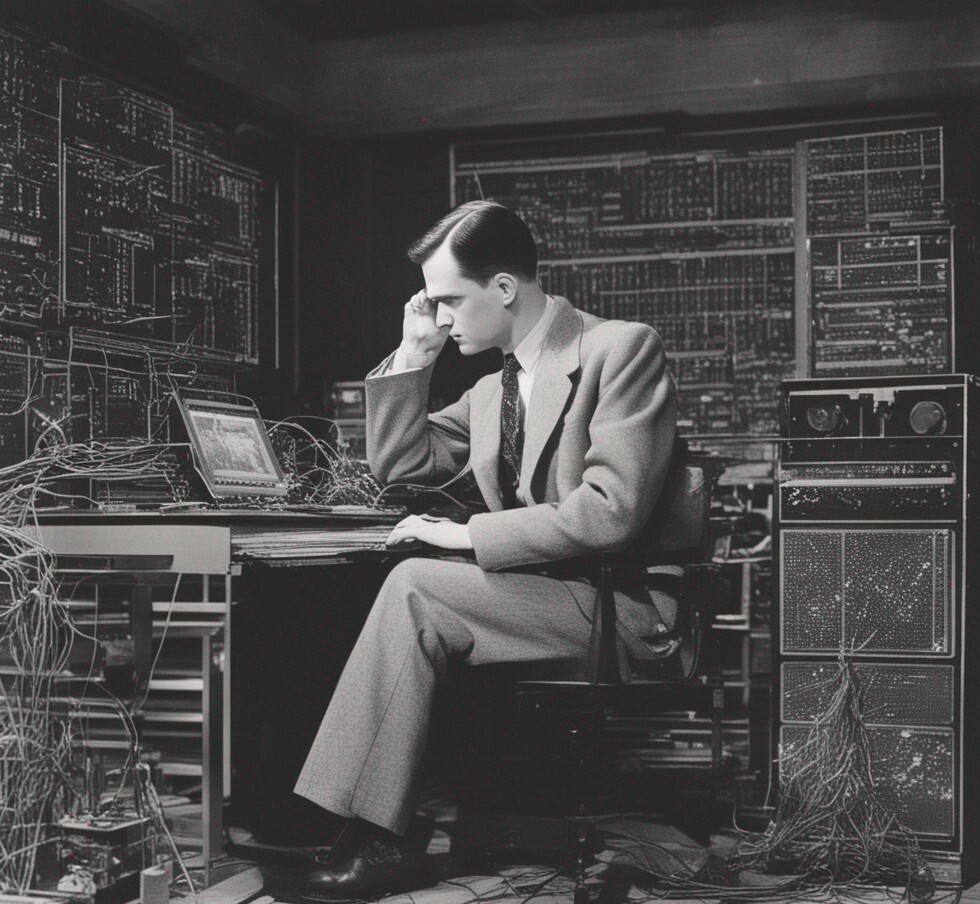
\includegraphics[width=0.9\linewidth]{img/turing_2.jpg}
    \caption{Prompt: ``Alan Turing, preparing for his upcoming Machine Learning Interview, cinematic, analog film''. Source: Clipdrop by stability.ai.}
    \label{fig:enter-label}
\end{figure}

\newpage

\clearpage % or \newpage

\section{Math}
\subsection{Algebra and (little) calculus}
\subsubsection{Vectors}

\begin{QandA}
    \item Dot product
    \begin{InnerQandA}
        \item What’s the geometric interpretation of the dot product of two vectors?
        \begin{answer}
            Multiplication of the length of one vector and the length of the projection of the other vector onto the first one.
        \end{answer}
        
        \item Given a vector $u$, find vector $v$ of unit length such that the dot product of $u$ and $v$ is maximum.
        \begin{answer}
            $$v = \frac{u}{\Vert u \Vert}$$
        \end{answer}
    \end{InnerQandA}

    \item Outer product
    \begin{InnerQandA}
        \item Given two vectors $a=[3,2,1]$ and $b=[-1,0,1]$. Calculate the outer product $a^T b$?  
        \begin{answer}
            \begin{align*}
                a^T b &= \begin{bmatrix}
                -3 & 0 & 3\\
                -2 & 0 & 2 \\
                -1 & 0 & 1
                \end{bmatrix}
            \end{align*}
        \end{answer}
        
        \item Give an example of how the outer product can be useful in ML.
        \begin{answer}
            The Covariance matrix is a commonly used quantity in Machine Learning algorithms (eg. PCA). Given a dataset $X \in \R^{n \times d}$ with $n$ samples and $d$ features, we calculate the (empirical) covariance as follows:
            \begin{align*}
                \Cov{X} = \frac{1}{n} \sum_{i=1}^n (x_i - \bar{x}) (x_i - \bar{x})^T
            \end{align*}
            where $\bar{x}$ is the mean feature vector: $\bar{x} = \frac{1}{n} \sum_{i=1}^n x_i$. 
        \end{answer}
    \end{InnerQandA}
    
    \item What does it mean for two vectors to be linearly independent?
    \begin{answer}
        Two vectors $a, b \in \R^n$ are linearly independent iff $a \neq c \cdot b$ for $c \in \R$.
    \end{answer}
    
    \item Given two sets of vectors $A = \{ a_1, a_2, \ldots, a_n\}$ and $B = \{b_1, b_2, \ldots, b_m\}$ how do you check if they share the same basis?
    \begin{answer}
         We should check if every vector in $B$ can be written as a linear combination of vectors in $A$. More precisely, for all $b_i \in B$ it should hold that:
         \begin{align*}
             b_i = \gamma_1^i a_1 + \gamma_2^i a_2 + \ldots + \gamma_n^i a_n
         \end{align*}
         where $\gamma_1^i, \gamma_2^i, \ldots, \gamma_n^i$ are some scalars.
    \end{answer}
    
    \item Given $n$ vectors, each of $d$ dimensions. What is the dimension of their span?
    \begin{answer}
        The dimension of their span is the number of linearly independent vectors. 
    \end{answer}

    \item Norms and metrics
    \begin{InnerQandA}
        \item What's a norm? What is $L_0$, $L_1$, $L_2$, \ldots, $L_p$ norm?
        \begin{answer}
            A norm is a function $\Vert \cdot \Vert: X \rightarrow \R$, where $X$ is a vector space, that satisfies the following properties:
            \begin{enumerate}[label={N.\arabic*.}]
                \item Triangle inequality: $\Vert x + y \Vert \le \Vert x \Vert + \Vert y \Vert$
                \item Absolute homogeneity: $\Vert cx \Vert = \vert c \vert \Vert x \Vert $, where $c \in \R$
                \item $x = 0 \implies \Vert x \Vert = 0 $ 
                \item $\Vert x \Vert \implies x = 0$
            \end{enumerate}
            $\Vert \cdot \Vert$ is a semi-norm if only N.1 - N.3 are satisfied. In general, we define the $p$-norm as follows:
            \begin{align*}
                \Vert x \Vert_p := \left( \sum_{i=1}^d x_i^p \right)^{\frac{1}{p}}
            \end{align*}
            Finally, we define the two special norms:
            \begin{align*}
                \Vert x \Vert_\infty := \max_{i} \vert x_i \vert \\
                \Vert x \Vert_0 := \sum_{i=1}^d \mathbbm{1}_{\{ x_i \neq 0 \}}
            \end{align*}
        \end{answer}

        \item How do norm and metric differ? Given a norm, make a metric. Given a metric, can we make a norm?
        \begin{answer}
            A metric is a function $d: \mathbb{X} \times \mathbb{X} \rightarrow \R$ if: 
            \begin{enumerate}[label={M.\arabic*.}]
                \item Non-negativity: $d(x, y) > 0 \text{ if } x \neq y \text{ else } d(x,y) = 0$ 
                \item Triangle inequality: $d(x, y) \le d(x, z) + d(z, y)$
                \item Symmetry: d(x, y) = d(y, x)
            \end{enumerate}
            A norm can always induce a metric: 
            \begin{align*}
                d(x, y) := \Vert x - y \Vert 
            \end{align*}
            The other direction does not work in general.
        \end{answer}
    \end{InnerQandA}
    
\end{QandA}

\subsubsection{Matrices}
\begin{QandA}
    \item Why do we say that matrices are linear transformations?
    \begin{answer}
        They are called linear transformations because they preserve vector addition and scalar multiplication:
        \begin{align*}
            A(x+y) = Ax + Ay \\
            A(c \cdot x) = c \cdot (Ax)
        \end{align*}
    \end{answer}
    
    \item What’s the inverse of a matrix? Do all matrices have an inverse? Is the inverse of a matrix always unique?
    \begin{answer}
        A matrix $A \in \R^{n \times n}$ is called \textit{invertible} if there exists a matrix $B \in \R^{n \times n}$ s.t. $AB = BA = I$. The inverse of a matrix is unique. A square matrix that does not have an inverse is called \textit{singular}. A square matrix is singular iff its determinant is 0. Furthermore, non-square matrices do not have an inverse.
    \end{answer}
    
    \item What does the determinant of a matrix represent?
    \begin{answer}
        The \textit{determinant} of a matrix is a function $\det(\cdot): \R^{n \times n} \rightarrow \R$ which outputs the change in (signed) "volume" represented by the transformation of the standard basis to the columns of $A$.
    \end{answer}
    
    \item What happens to the determinant of a matrix if we multiply one of its rows by a scalar?
    \begin{answer}
        The determinant is \textit{multilinear}: If the $j$-th column/row of a matrix $A$ is written as a linear combination $a_j = r \cdot v + w$ of two column vectors $v$ and $w$, and a scalar $r$, then the determinant of $A$ can be expressed as follows:
        \begin{align*}
            \vert A \vert &= \vert a_1, \ldots, a_{j-1}, a_j, a_{j+1}, \ldots, a_n \vert \\
            &= \vert a_1, \ldots, a_{j-1}, r \cdot v + w, a_{j+1}, \ldots, a_n \vert \\
            &= r \cdot \vert a_1, \ldots, v, \ldots, a_n \vert + \vert a_1, \ldots, w, \ldots, a_n \vert 
        \end{align*}
    \end{answer}
    
    \item A $4 \times 4$ matrix has four eigenvalues $3,3,2,-1$. What can we say about the trace and the determinant of this matrix?
    \begin{answer}
        The trace is the sum of the eignevalues: $3+3+2-1 = 7$. \\
        The determinant is the product of the eigenvalues: $3 \cdot 3 \cdot 2 \cdot (-1) = -18$.
    \end{answer}
    
    \item Given the following matrix:
    \begin{align*}
        \begin{bmatrix}
        1 & 4 & -2 \\
        -1 & 3 & 2 \\
        3 & 5 & -6
    \end{bmatrix}
    \end{align*}
    Without explicitly using the equation for calculating determinants, what can we say about this matrix’s determinant? (Hint: rely on a property of this matrix to determine its determinant)
    \begin{answer}
        The third column equals (-2) $\times$ the first column, which means they are linearly dependent. As such, one of the eigenvalues will be 0. Since the determinant equals the factorisation of all eigenvalues, it will be 0 as well. 
    \end{answer}
    
    \item What’s the difference between the Covariance matrix  $A^TA$ and the Gram matrix $AA^T$ ?
    \begin{answer}
        Suppose $A \in \R^{n \times d}$, corresponding to $n$ samples with each having $d$ features. Then, the Covariance matrix $A^TA \in \R^{d \times d}$ captures the "distance" between features, whereas the Gram matrix $AA^T \in \R^{n \times n}$ captures the "distance" between samples.
    \end{answer}
    
    \item Given $A \in \R^{n \times m}$ and $b \in \R^n$:
    \begin{InnerQandA}
        \item Find $x$ such that $Ax = b$.
        \begin{answer}
            If $A$ is square and has full rank, then: $x = A^{-1}b$.
        \end{answer}
        
        \item When does this have a unique solution?
        \begin{answer}
            In a set of linear simultaneous equations, a unique solution exists if and only if: 
            \begin{itemize}
                \item the number of unknowns and the number of equations are equal
                \item all equations are consistent
                \item there is no linear dependence between any two or more equations, that is, all equations are independent.
            \end{itemize}
        \end{answer}
        
        \item Why is it when $A$ has more columns than rows,  $Ax=b$ has multiple solutions?
        \begin{answer}
            Each unknown can be seen as an available degree of freedom. Each equation introduced into the system can be viewed as a constraint that restricts one degree of freedom. \\
            Therefore, the critical case occurs when the number of equations and the number of free variables are equal -- for every variable giving a degree of freedom, there exists a corresponding constraint removing a degree of freedom. \\
            The underdetermined case, by contrast, occurs when the system has been underconstrained  -- that is, when the unknowns outnumber the equations.
        \end{answer}
        
        \item Given a matrix $A$ with no inverse. How would you solve the equation $Ax=b$ ? What is the pseudoinverse and how to calculate it?
        \begin{answer}
            For an arbitrary matrix $A \in \R^{m \times n}$, its pseudoinverse $A^{\#} \in \R^{n \times m}$ is a matrix that satisfies the following criteria:
            \begin{itemize}
                \item $A A^{\#} A = A$
                \item $A^{\#} A A^{\#} = A^{\#}$
                \item $(A A^{\#})^T = A A^{\#}$
                \item $(A^{\#} A)^T = A^{\#} A$
            \end{itemize}
            Back to our system of linear equations, regardless of whether $A$ is square and regardless of the rank of $A$, all solutions (if any exist) can be obtained using the pseudoinverse:
            \begin{align*}
                x = A^{\#} b + (I - A^{\#}A)w
            \end{align*}
            where $w$ is a vector of free parameters that ranges over all possible $n \times 1$ vectors. A necessary and sufficient condition for any solution(s) to exist is that the potential solution obtained using $w=0$ satisfy $Ax = b$, that is: $A A^{\#}b = b$ (substitute $x = A^\# b$ in $Ax = b$). If this condition does not hold, the equation system is inconsistent and has no solution. If the condition holds, the system is consistent and at least one solution exists. For example, in the above-mentioned case in which $A$ is square and of full rank, $A^{\#}$ simply equals $A^{-1}$ and the general solution equation simplifies to:
            \begin{align*}
                x = A^{-1}b + (I - A^{-1}A)w = A^{-1}b + (I - I)w = A^{-1}b
            \end{align*}
            as previously stated, where $w$ has completely dropped out of the solution, leaving only a single solution. In other cases though, $w$ remains and hence an infinitude of potential values of the free parameter vector $w$ give an infinitude of solutions of the equation.
        \end{answer}
    \end{InnerQandA}
    
    \item Derivative is the backbone of gradient descent.
    \begin{InnerQandA}
        \item What does the derivative represent?
        \begin{answer}
            The derivative of a function measures the sensitivity to change in the function output with respect to a change in the input. \\
            Moreover, when it exists, the derivative at a given point is the \textit{slope} of the tangent line to the graph of the function at that point. The tangent line is the best \textit{linear approximation} of the function at that input value. This is the reason why in gradient descent we (slowly) move in the (negative) direction of the derivative. 
        \end{answer}
        \item What’s the difference between derivative, gradient, and Jacobian?
        \begin{answer}
            \begin{itemize}
                \item When $f: \R \rightarrow \R$, we calculate the derivative $\frac{df}{dx}$.
                \item When $f: \R^n \rightarrow \R$, we calculate the gradient:
                \begin{align*}
                    \nabla_x f = 
                    \begin{bmatrix}
                     \frac{\partial f}{ \partial x_1} & \frac{\partial f}{ \partial x_2} & \ldots  & \frac{\partial f}{ \partial x_n}
                    \end{bmatrix}
                \end{align*}
                \item When $f: \R^n \rightarrow \R^m$, we calculate the Jacobian:
                \begin{align*}
                    \Jac_x(f) = 
                    \begin{bmatrix}
                     \frac{\partial f_1}{ \partial x_1} & \ldots & \frac{\partial f_1}{ \partial x_n} \\
                     \vdots & \ddots & \vdots \\
                     \frac{\partial f_m}{ \partial x_1} & \ldots & \frac{\partial f_m}{ \partial x_n}
                    \end{bmatrix}
                \end{align*}
            \end{itemize}
        \end{answer}
    \end{InnerQandA}
    
    \item Say we have the weights $w \in \R^{d \times m}$ and a mini-batch $x$ of $n$ elements, each element is of the shape $1 \times d$ so that $x \in \R^{n \times d}$. We have the output $y = f(x; w) = xw$. What's the dimension of the Jacobian $\frac{\partial y}{\partial x}$?
    \begin{answer}
        First, notice that $y \in \R^{n \times m}$. With that said, $\Jac_x(f) \in \R^{(n \times m) \times (n \times d)}$, or equivalently $\Jac_x(f) \in \R^{(n \cdot m) \times (n \cdot d)}$, given that we have reshaped the 4-dim tensor into a 2-dim tensor, i.e. a matrix.
    \end{answer}
    
    \item Given a very large symmetric matrix $A$ that doesn't fit into memory, say $A \in \R^{1M \times 1M}$ and a function $f$ that can quickly compute $f(x) = Ax$ for $x \in \R^{1M}$. Find the unit vector $x$ so that $x^T A x$ is minimal. (Hint: Can you frame it as an optimization problem and use gradient descent to find an approximate solution?).
    
    \begin{answer}
        Since this is a constrained optimization problem, we can turn it into an unconstrained one by using a Lagrange multiplier:
        \begin{align*}
            L(x, \lambda) = x^T A x + \lambda (x^t x - 1) 
        \end{align*}
        The critical points of Lagrangians occur at saddle points, rather than at local minima. Unfortunately, methods such as gradient descent which are designed to find local minima (or maxima) cannot be applied directly. For this reason, we must either use an optimization technique that stationary points that are not necessarily extrema (such as Newton's method without an extremum seeking line search), or we modify the formulation to ensure that it's a minimization problem. \\\\
        For the purpose of our problem, let us use the latter solution. First, let us compute the gradients:
        \begin{align*}
            \frac{\partial L}{ \partial x} &= 2Ax + 2 \lambda x \in \R^n \\ 
            \frac{\partial L}{\partial \lambda} &= x^T x - 1 \in \R
        \end{align*}
        Next, we stack them into a single column vector:
        \begin{align*}
            \nabla_{x, \lambda}L = 
            \begin{bmatrix}
             \frac{\partial L}{\partial x} \\
             \\
             \frac{\partial L}{\partial \lambda}
            \end{bmatrix} \in \R^{n + 1}
        \end{align*}
        Finally, we minimize the (squared) magnitude of the gradient:
        \begin{align*}
            x^{*}, \lambda^{*} &= \argmin_{x, \lambda} \sqrt{(\nabla_{x, \lambda}L)^T (\nabla_{x, \lambda}L)} \\
             &= \argmin_{x, \lambda} \underbrace{(\nabla_{x, \lambda}L)^T (\nabla_{x, \lambda}L)}_{\ge 0}
        \end{align*}
        At the optimal $x^{*}$, $\lambda^{*}$ we have $ \Vert \nabla_{x, \lambda}L \Vert ^2 \approx 0$, meaning that all partial derivatives are approximately $0$. Therefore, they are a solution to the original optimization problem $L(x, \lambda)$. Unlike the critical points in $L$ however, $x^{*}$ and $\lambda^{*}$ occur at local minima (instead of at saddle points), so numerical optimization techniques (such as gradient descent) can be used to find them. 
        
        (Source: \href{https://en.wikipedia.org/wiki/Lagrange_multiplier#Examples}{Wikipedia})
    \end{answer}
\end{QandA}

\subsubsection{Dimensionality reduction}
\begin{QandA}
    \item Why do we need dimensionality reduction?
    \begin{answer}
        \textbf{Curse of dimensionality} -- When the dimensionality increases, the volume of the space increases so fast that the available data become sparse. In order to obtain a reliable result, the amount of data needed often grows exponentially with the dimensionality. Also, organizing and searching data often relies on detecting areas where objects form groups with similar properties; in high dimensional data, however, all objects appear to be sparse and dissimilar in many ways, which prevents common data organization strategies from being efficient.
    \end{answer}

    \item Eigendecomposition is a common factorization technique used for dimensionality reduction. Is the eigendecomposition of a matrix always unique?
    \begin{answer}
        The decomposition is not always unique. Suppose $A \in \R^{2 \times 2}$ has two equal eigenvalues $\lambda_1 = \lambda_2 = \lambda$, with corresponding eigenvectors $u_1, u_2$. Then:
        \begin{align*}
            A u_1 &= \lambda_1 u_1 = \lambda u_1 \\
            A u_2 &= \lambda_2 u_2 = \lambda u_2
        \end{align*}
        Or written in matrix form:
        \begin{align*}
            A \begin{bmatrix}
                u_1 & u_2
            \end{bmatrix}
             &= \begin{bmatrix}
                u_1 & u_2
            \end{bmatrix} 
            \begin{bmatrix}
                \lambda & 0 \\
                0 & \lambda
            \end{bmatrix}
        \end{align*}
        Notice that we can permute the matrix of eigenvectors (thus obtaining a different factorization):
        \begin{align*}
            A \begin{bmatrix}
                u_2 & u_1
            \end{bmatrix}
             &= \begin{bmatrix}
                u_2 & u_1
            \end{bmatrix} 
            \begin{bmatrix}
                \lambda & 0 \\
                0 & \lambda
            \end{bmatrix}
        \end{align*}
        But we still end up with the same eigen-properties:
        \begin{align*}
            A u_2 &= \lambda u_2 \\
            A u_1 &= \lambda u_1
        \end{align*}
    \end{answer}
    \item Name some applications of eigenvalues and eigenvectors.
    \begin{answer}
        Principal Component Analysis (PCA), Spectral Clustering, Low rank factorization / rank-k approximation of a matrix (eg. image compression), Estimating curvature of the loss through the eigenvalues of the Hessian... 
    \end{answer}

    \item We want to do PCA on a dataset of multiple features in different ranges. For example, one is in the range 0-1 and one is in the range 10 - 1000. Will PCA work on this dataset?
    \begin{answer}
         In PCA we are interested in the components that maximize the variance. If one component (e.g. human height) varies less than another (e.g. weight) because of their respective scales (meters vs. kilos), PCA might determine that the direction of maximal variance more closely corresponds with the ‘weight’ axis, if those features are not scaled. Since a change in height of one meter should be considered much more important than the change in weight of one kilogram, the previous assumption would be incorrect. Therefore, it is important to standardize the features before applying PCA (source: \href{https://scikit-learn.org/stable/auto_examples/preprocessing/plot_scaling_importance.html}{scikit}).
    \end{answer}

    \item Under what conditions can one apply eigendecomposition? What about SVD?
    \begin{answer}
        Eigendecomposition is possible only for (square) diagonalizable matrices. On the other hand, the Singular Value Decomposition (SVD) always exists (even for non-square matrices).
    \end{answer}
    \begin{InnerQandA}
        \item What is the relationship between SVD and eigendecomposition?
        \begin{answer}
            Consider $A \in \R^{m \times n}$ of rank $r$. Then, we can factorize $A$ as follows:
            \begin{align*}
                A = U \Sigma V^T
            \end{align*}
            where $U \in \R^{m \times m}$ is an orthogonal matrix of left singular vectors, $V \in \R^{n \times n}$ is an orthogonal matrix of right singular vectors, and $\Sigma \in \R^{m \times n}$ is "diagonal" matrix of singular values s.t. exactly $r$ of the values $\sigma_i := \Sigma_{ii}$ are non-zero. By construction:
            \begin{itemize}
                \item The left singular vectors of $A$ are the eigenvectors of $AA^T$. From the Spectral Theorem, the eigenvectors (and thus the left singular vectors) are orthonormal.
                \item The right singular vectors of $A$ are the eigenvecotrs of $A^TA$. From the Spectral Theorem, the eigenvectors (and thus the right singular vectors) are orthonormal.
                \item If $\lambda$ is an eigenvalue of $AA^T$ (or $A^TA)$, then $\sqrt{\lambda}$ is a singular value of $A$. From the positive-semidefinitness of $AA^T$ (or $A^TA$), the eigenvalues (and thus the singular values) are non-negative.
            \end{itemize}
        \end{answer}

        \item What’s the relationship between PCA and SVD?
        \begin{answer}
            Suppose we have data $X \in \R^{n \times d}$ with $n$ samples and $d$ features. Moreover, assume that the data has been centered s.t. the mean of each feature is $0$. Then, we can perform PCA in two main ways:
            \begin{itemize}
                \item First we compute the covariance matrix $C = \frac{1}{(n-1)} X^T X \in \R^{d \times d}$, and perform eigendecomposition: $C = V L V^T$, with eigenvalues as the diagonal of $L \in \R^{d \times d}$, and eigenvectors as the columns of $V \in \R^{d \times d}$. Then, we stack the $k$ eigenvectors of $V$ corresponding to the top $k$ eigenvalues into a matrix $\tilde{V} \in \R^{d \times k}$. Finally, we obtain the component values as follows: $\tilde{X} = X \tilde{V} \in \R^{n \times k}$.
                \item Alternatively, instead of first computing the covariance matrix and then performing eigendecomposition, notice that given the above formulation, we can directly compute SVD on the data matrix $X$, thus obtaining: $X = U \Sigma V^t$. By construction, the right singular vectors in $V$ are the eigenvectors of $X^TX$. Similarly, we stack the $k$ right singular vectors corresponding to the top $k$ singular values into a matrix $\tilde{V} \in \R^{d \times k}$. Finally, we obtain the component values as follows: $\tilde{X} = X \tilde{V} \in \R^{n \times k}$.
            \end{itemize}

            Even though SVD is slower, is often considered to be the preferred method because of its higher numerical accuracy.
            
            (See more \href{https://stats.stackexchange.com/questions/79043/why-pca-of-data-by-means-of-svd-of-the-data}{here})
        \end{answer}
    \end{InnerQandA}

    \item How does t-SNE (T-distributed Stochastic Neighbor Embedding) work? Why do we need it?

    \begin{answer}
        t-SNE is a statistical method for visualizing high-dimensional data by giving each datapoint a location in a two or three-dimensional map. Specifically, it models each high-dimensional object by a two- or three-dimensional point in such a way that similar objects are modeled by nearby points and dissimilar objects are modeled by distant points with high probability. \\\\
        First, t-SNE constructs a probability distribution over pairs of high-dimensional objects in such a way that similar objects are assigned a higher probability while dissimilar points are assigned a lower probability. In particular, given a set of $N$ high-dimensional objects $x_1, \ldots, x_N$, t-SNE computes:
        \begin{align*}
            p_{j \mid i} = \frac{\exp(- \Vert x_i - x_j\Vert^2/2\sigma_i^2)}{\sum_{k \neq i} \exp(- \Vert x_i - x_k\Vert^2/2\sigma_i^2)}
        \end{align*}
        and sets $p_{i \vert i} = 0$. Note that $\sum_j p_{j \vert i} = 1$ for all $i$. Then, it computes:
        \begin{align*}
            p_{ij} = \frac{p_{j \vert i} + p_{i \vert j}}{2N}
        \end{align*}
    Note that $p_{ij} = p_{ji}, p_{ii} = 0, \sum_{i,j} p_{ij} = 1$. The similarity of datapoint $x_j$ to datapoint $x_i$ is the conditional probability $p_{j \vert i}$ that $x_i$ would pick $x_j$ as its neighbor if neighbors were picked in proportion to their probability density under a Gaussian centered at $x_i$. \\\\
    Second, t-SNE defines a similar probability distribution over the points in the low-dimensional map. In particular, it aims to learn $d$-dimensional map $y_1, \ldots, y_N$ (where $d$ is chosen 2 or 3) that reflects the similarities $p_{ij}$ as well as possible. To this end, it measures similarities $q_{ij}$ between two points $y_i$ and $y_j$ using:
    \begin{align*}
        q_{ij} = \frac{(1 + \Vert y_i - y_j \Vert^2)^{-1}}{\sum_k \sum_{l \neq k} (1 + \Vert y_k - y_l \Vert^2)^{-1}}
    \end{align*}
    and set $q_{ii} = 0$. Herein a heavy-tailed Student t-distribution (with one-degree of freedom, which is the same as a Cauchy distribution) is used to measure similarities between low-dimensional points in order to allow dissimilar objects to be modeled far apart in the map. \\\\
    Finally, the locations $y_i$ in the map are determined by minimizing the Kullback-Leibler divergence of the distribution $P$ from the distribution $Q$:
    \begin{align*}
        \KL{P}{Q} = \sum_{i \neq j} p_{ij} \log \frac{p_{ij}}{q_{ij}}
    \end{align*}
    The minimization of the KL divergence wrt the points $y_i$ is performed using gradient descent.  \\\\
    While t-SNE plots often seem to display clusters, the visual clusters can be influenced strongly by the chosen parameterization and therefore a good understanding of the parameters for t-SNE is necessary. Such "clusters" can be shown to even appear in non-clustered data, and thus may be false findings. Interactive exploration may thus be necessary to choose parameters and validate results. 
    
    (Source: \href{https://en.wikipedia.org/wiki/T-distributed_stochastic_neighbor_embedding}{Wikipedia})
    \end{answer}
\end{QandA}

\subsubsection{Calculus and convex optimization}
\begin{QandA}
    \item Differentiable functions
    \begin{InnerQandA}
        \item What does it mean when a function is differentiable?
        \begin{answer}
            A function $f: U \rightarrow \R$ is said to be differentiable at $a \in U$ if the derivative:
            \begin{align*}
                f'(a) = \lim_{h \rightarrow 0} \frac{f(a+h) - f(a)}{h}
            \end{align*}
            exists. This implies that the function is continuous at $a$. Note that every continuous function is not necessarily differentiable.
        \end{answer}

        \item Give an example of when a function doesn’t have a derivative at a point.  
        \begin{answer}
            Any non-continuous function. For example,
            \begin{align*}
                f(x) =
                    \begin{cases}
                    x^2 & \text{if } x \le 0\\
                    1+x & \text{otherwise}
                    \end{cases}
            \end{align*}
            is not differentiable at $x=0$.
        \end{answer}

        \item Give an example of non-differentiable functions that are frequently used in machine learning. How do we do backpropagation if those functions aren’t differentiable?
        \begin{answer}
            Some non-differentiable functions commonly used in Machine Learning: 
            \begin{align*}
                    f(x) &= \vert x \vert \\
                    \text{ReLU}(x) &= \begin{cases}
                    x & \text{if } x \ge 0\\
                    0 & \text{otherwise}
                    \end{cases} \\
                    \text{LeakyReLU}(x) &= \begin{cases}
                    x & \text{if } x \ge 0\\
                    \alpha x & \text{otherwise}
                    \end{cases} \\
            \end{align*}
            Each of these functions are not differentiable at $x=0$. In theory, since any finite set of points is a set of measure $0$, we have $p(x=0)$ and therefore can disregard that these functions are not differentiable. In practice however, due to finite precision it can occur that $x=0$. In these cases we can use a "faux" derivative -- by usually picking the left or the right derivative at the given point.
            
        \end{answer}
        
    \end{InnerQandA}

    \item Convexity
    \begin{InnerQandA}
        \item What does it mean for a function to be convex or concave? Draw it.
        \begin{answer}
            A function is called convex if the line segment between any two points on the graph of the function lies above the graph between the two points. More precisely, the function $f: X \rightarrow \R$ is convex if and only if for all $0 \le t \le 1$ and all $x_1, x_2 \in X$:
            \begin{align*}
                f(t x_1 + (1-t)x_2) \le t f(x_1) + (1-t)f(x_2)
            \end{align*}
        \end{answer}
        The function $f$ is said to be concave if $-f$ is convex.

        \item Why is convexity desirable in an optimization problem?
        \begin{answer}
            Convexity is desirable because any local minimum of a convex function is also a global minimum.
        \end{answer}

        \item Show that the cross-entropy loss function is convex.
        \begin{answer}
            We will prove that $\CE{P}{Q}$ is convex in $Q$, since typically $P$ is the ground-truth probability distribution and $Q$ is the predicted distribution of our model. For the purpose of this task, we have to show two results: the Log sum inequality, and the convexity of the KL divergence. 
            \begin{theorem}
                Let $a_1, \ldots, a_n$ and $b_1, \ldots, b_n$ be non-negative real numbers, and define $a = \sum_{i=1}^n a_i$ and $b = \sum_{i=1}^n b_i$. Then, the log sum inequality that:
                \begin{align*}
                    \sum_{i=1}^n \log \frac{a_i}{b_i} \ge a \log \frac{a}{b}
                \end{align*}
            \end{theorem}

            \begin{proof}
                Let $f(x) = x \log x$. Then, we re-write:
                \begin{align*}
                    \sum_{i=1}^n a_i \log \frac{a_i}{b_i} &= \sum_{i=1}^n b_i f \left(\frac{a_i}{b_i} \right) \\
                    &= b \sum_{i=1}^n \frac{b_i}{b} f \left( \frac{a_i}{b_i} \right)
                \end{align*}
            
                Because $f(x)$ is a convex function, and:
                \begin{align*}
                    \frac{b_i}{b} &\ge 0 \\
                    \sum_{i=1}^n \frac{b_i}{b} &= 1
                \end{align*}
                applying the Jensen's inequality yields:
                \begin{align*}
                    b \sum_{i=1}^n \frac{b_i}{b} f \left( \frac{a_i}{b_i} \right) & \ge b f \left( \sum_{i=1}^n \frac{b_i}{b} \frac{a_i}{b_i} \right) \\
                    &= b f \left( \frac{1}{b} \sum_{i=1}^n a_i \right) \\
                    &= b f \left( \frac{a}{b} \right) \\
                    &= a \log \frac{a}{b}
                \end{align*}
                Therefore, we obtain the \textbf{Log sum inequality}:
                \begin{align*}
                    \sum_{i=1}^n a_i \log \frac{a_i}{b_i} \ge a \log \frac{a}{b}
                \end{align*}
            \end{proof}

            \begin{theorem}
                The Kullback-Leibler divergence is convex in the pair of probability distributions $(p, q)$, i.e.
                \begin{align*}
                    \KL{\lambda p_1 + (1-\lambda)p_2}{\lambda q + (1-\lambda)q_2} \le \lambda \KL{p_1}{q_1} + (1-\lambda)\KL{p_2}{q_2}
                \end{align*}
            \end{theorem}
            \begin{proof}
                The Kullback-Leibler divergence of $P$ from $Q$ is defined as:
                \begin{align*}
                    \KL{P}{Q} = \sum_{x} p(x) \log \frac{p(x)}{q(x)}
                \end{align*}
                Now:
                \begin{align}
                    &\KL{\lambda p_1 + (1-\lambda)p_2}{\lambda q + (1-\lambda)q_2} \\
                    = &\sum_{x}\left[ \left[\lambda p_1(x) + (1-\lambda)p_2(x)\right] \cdot \log \frac{\lambda p_1(x) + (1-\lambda)p_2(x)}{\lambda q_1(x) + (1-\lambda)q_2(x)} \right] \\
                    \le &\sum_x \left[ \lambda p_1(x) \log \frac{\lambda p_1(x)}{\lambda q_1(x)} + (1 - \lambda) p_2(x) \log \frac{(1-\lambda) p_2(x)}{(1-\lambda) q_2(x)} \right] \\
                    = &\lambda \sum_x p_1(x) \log \frac{ p_1(x)}{q_1(x)} + (1 - \lambda) \sum_x p_2(x) \log \frac{p_2(x)}{q_2(x)}  \\
                    = &\lambda \KL{p_1}{q_1} + (1-\lambda) \KL{p_2}{q_2}
                \end{align}
                Where in (3) we use the Log sum inequality with:
                \begin{align*}
                    a_1 &= \lambda p_1(x) & a_2 = (1-\lambda) p_2(x)\\
                    b_1 &= \lambda q_1(x) & b_2 = (1-\lambda) q_2(x)\\
                \end{align*}
            \end{proof}
        Finally, going back to the original task of proving the convexity of $\CE{P}{Q}$ in $Q$, let us first decompose the cross-entropy:
        \begin{align*}
            \CE{P}{Q} &= \Ent{P} + \KL{P}{Q}
        \end{align*}
        Since $\Ent{P}$ is constant wrt. $Q$, and we showed that $\KL{P}{Q}$ is convex wrt. both $P$ and $Q$, we can deduce that $\CE{P}{Q}$ is convex wrt. $Q$.
        
        (Source: \href{https://statproofbook.github.io/P/entcross-conv}{The Book of Statistical Proofs})
        \end{answer}
    \end{InnerQandA}

    \item Given a logistic discriminant classifier:
    \begin{align*}
        p(y=1 \vert x) = \sigma(w^tx)
    \end{align*}
    where the sigmoid function is given by:
    \begin{align*}
        \sigma(z) = (1 + \exp(-z))^{-1} 
    \end{align*}
    The logistic loss for training sample $x_i$ with class label $y_i$ is given by:
    \begin{align*}
        L(y_i, x_i; w) = -y_i \log p(y_i \vert x_i)
    \end{align*}
    (Note: I believe in the book $y_i$ is missing from the loss $L$)
    
    \begin{InnerQandA}
        \item Show that $p(y=-1 \vert x) = \sigma (-w^t x)$.
        \begin{answer}
            \begin{align*}
                p(y=-1 \vert x) &= 1 - p(y=1 \vert x) \\
                &= 1 - \frac{1}{1 + \exp(-w^tx)} \\
                &= \frac{1 + \exp(-w^tx) - 1}{1 + \exp(-w^tx)} \\ 
                &= \frac{\exp(-w^tx)}{1 + \exp(-w^tx)} \\ 
                &= \frac{1}{\exp(w^tx)(1 + \exp(-w^tx))} \\
                &= \frac{1}{\exp(w^tx) + 1} \\
                &= \sigma (-w^t x)
            \end{align*}
        \end{answer}

        \item Show that $\nabla_w L (y_i, x_i; w) = -y_i (1 - p(y_i \vert x_i))x_i$.

        \begin{answer}
            We have the following computation graph:
            \begin{align*}
                z &= w^t x \\
                \sigma(z) &= \frac{1}{1 + \exp(-z)} \\
                L(y_i, x_i; w) &= -y_i \log \sigma(z)
            \end{align*}
            Therefore, using the chain rule we can decompose the derivative as follows:
            \begin{align*}
                \frac{\partial L}{\partial w} &= \frac{\partial L}{\partial \sigma} \cdot \frac{\partial \sigma}{\partial z} \cdot \frac{\partial z}{\partial w}
            \end{align*}
            Let's compute each term separately:
            \begin{align*}
                \frac{\partial L}{\partial \sigma} &= -\frac{y_i}{\sigma(z)} \\
                \frac{\partial \sigma(z)}{\partial(z)} &= \frac{\partial}{\partial z} \left( \frac{1}{1 + \exp(-z)} \right) = -\frac{1}{(1 + \exp(-z))^2} (-\exp(-z)) = \frac{1}{1+ \exp(-z)} \cdot \frac{\exp(-z)}{1 + \exp(-z)} \\
                &= \frac{1}{1+ \exp(-z)} \cdot  \frac{\exp(-z) + 1 - 1}{1 + \exp(-z)} = \frac{1}{1+ \exp(-z)} \cdot \left( 
                1 - \frac{1}{1+ \exp(-z)} \right) = \sigma(z)(1 - \sigma(z)) \\
                \frac{\partial z}{\partial w} &= \frac{\partial}{\partial w} \left( w^w x \right) = x
            \end{align*}
            Therefore:
            \begin{align*}
                \frac{\partial L}{\partial w} &= \frac{\partial L}{\partial \sigma} \cdot \frac{\partial \sigma}{\partial z} \cdot \frac{\partial z}{\partial w} = -\frac{y_i}{\sigma(z)} \cdot \sigma(z)(1 - \sigma(z)) \cdot x = -y_i (1 - \sigma(z)) x 
            \end{align*}
        \end{answer}

    \item Show that $\nabla_w L (y_i, x_i; w)$ is convex.
    \begin{answer}
        \todo
    \end{answer}
    \end{InnerQandA}

    \item Most ML algorithms we use nowadays use first-order derivatives (gradients) to construct the next training iteration.
    \begin{InnerQandA}
        \item How can we use second-order derivatives for training models?
        \begin{answer}
            Given a twice differentiable function $f: \R \rightarrow \R$ we seek to solve the optimization problem:
            \begin{align*}
                \min_{x \in \R} f(x)
            \end{align*}
            Newton's method approaches this problem in an iterative fashion by constructing a sequence $\left\{ x_k \right\}$ that converges towards the minimizer $x^{*}$ of f. In particular, it performs second-order Taylor approximation of $f$ around $x_k$:
            \begin{align*}
                f(x_k + t) \approx f(x_k) + f'(x_k)t + \frac{1}{2} f''(x_k)t^2
            \end{align*}
            The next iterate $x_{k+1}$ is defined as to minimize this quadratic approximation in t, and setting $x_{k+1} = x_k + t$. If the second derivative is positive, the quadratic approximation is a convex function of $t$, and its minimum can be found by setting the derivative to zero. More precisely:
            \begin{align*}
                0 = \frac{d}{dt} \left( f(x_k) + f'(x_k)t + \frac{1}{2} f''(x_k)t^2 \right) = f'(x_k) + f''(x_k)t
            \end{align*}
            Therefore, the minimum of the quadratic approximation is achieved for:
            \begin{align*}
                t = -\frac{f'(x_k)}{f''(x_k)}
            \end{align*}
            Putting everything together, the Newton's method performs the following iteration:
            \begin{align*}
                x_{k+1} = x_k + t = x_k -\frac{f'(x_k)}{f''(x_k)}
            \end{align*}
            (Source: \href{https://en.wikipedia.org/wiki/Newton%27s_method_in_optimization}{Wikipedia})
        \end{answer}

        \item Pros and cons of second-order optimization.
        \begin{answer}
            The advantage of the Newton optimization method is that in general it converges faster than pure gradient descent, since we perform a higher order local approximation (second order as opposed to first order), and therefore make a more informed choice about the next step in the descent. \\\\
            Nevertheless, it comes with several drawbacks as well:
            \begin{itemize}
                \item Finding the inverse of the Hessian in high dimensions can be an expensive operation. Several approximations exist: quasi-Newton methods, Levenberg-Marquardt algorithm, ...
                \item It does not work if the Hessian is not invertible.
                \item It may not converge at all, but can enter a cycle having more than 1 point.
                \item It can converge to a saddle point instead of to a local minimum.
            \end{itemize}
        \end{answer}

        \item Why don’t we see more second-order optimization in practice?
        \begin{answer}
            To further highlight the intractability of computing the Hessian, let us note that today's Deep Learning models are on the order of $10^{10}$ (some even $10^{12}$) parameters. Even with pure gradient descent, training these models requires a lot of engineering effort in order to distribute the computation across multitude of GPUs. Since the Hessian is quadratic in the number of parameters, it almost certainly isn't possible to scale the compute requirements with today's state of the hardware.
        \end{answer}

    \end{InnerQandA}

    \item How can we use the Hessian (second derivative matrix) to test for critical points?
    \begin{answer}
        Suppose we have $f \in \R^n \rightarrow \R$ and $a \in \R^n$ be a critical point for which the Hessian matrix is invertible. Then:
        \begin{itemize}
            \item If the Hessian is positive definite (equivalently, has all eigenvalues positive) at $a$, then $f$ attains a local minimum at $a$. 
            \item If the Hessian is negative definite (equivalently, has all eigenvalues negative) at $a$, then $f$ attains a local maximum at $a$.
            \item If the Hessian has both positive and negative eigenvalues, then $a$ is a saddle point for $f$.
        \end{itemize}
        In those cases not listed above, the test is inconclusive. 
        
        (Source: \href{https://en.wikipedia.org/wiki/Second_partial_derivative_test}{Wikipedia})
    \end{answer}

    \item Jensen’s inequality forms the basis for many algorithms for probabilistic inference, including Expectation-Maximization and variational inference. Explain what Jensen’s inequality is.
    \begin{answer}
        As stated before, for a given convex function $f$, we had the following property: 
        \begin{align*}
            g(tx_1 + (1-t)x_2) \le tg(x_1) + (1-t)g(x_2)
        \end{align*}

        Let us generalize this property. Again, suppose we have a convex function $f$, variables $x_1, \ldots, x_n \in I$, and non-negative real numbers $\alpha_1, \ldots, \alpha_n$ s.t. $\sum_i \alpha_i = 1$. Then, by induction we have:
        \begin{align*}
            g(\alpha_1 x_1 + \ldots + \alpha_n x_n) \le \alpha_1 g(x_1) + \ldots + \alpha_n g(x_n)
        \end{align*}

        Let's formalize it one step further. Consider a convex function $f$, a discrete random variable $X$ with $n$ possible values $x_1, \ldots, x_n$, and real non-negative values $a_i = p(X=x_i)$. Then, we  obtain the general form of the Jensen's inequality:
        \begin{align*}
            g(\Exp{X}) \le \Exp{g(X)}
        \end{align*}
        (Source: \href{https://www.probabilitycourse.com/chapter6/6_2_5_jensen's_inequality.php}{Introduction to Probability, Statistics, and Random Processes})
    \end{answer}

    \item Explain the chain rule.
    \begin{answer}
        The chain rule is a formula that expresses the derivative of the composition of two differentiable functions $f$ and $g$ in terms of the derivatives of $f$ and $g$. More precisely, if $h = f \circ g$ is the function such that $h(x) = f(g(x))$ for every $x$, then the chain rule is:
        \begin{align*}
            \frac{\partial h}{\partial x} = \frac{\partial f}{\partial g} \cdot \frac{\partial g}{\partial x}
        \end{align*}
        (Source: \href{https://en.wikipedia.org/wiki/Chain_rule}{Wikipedia})
    \end{answer}
    
    \item Let $x \in \R^n$, $L = CrossEntropy(Softmax(x), y)$, in which $y$ is a one-hot vector. Take the derivative of $L$ with respect to $x$.
    \begin{answer}
        First, let us expand the loss:
        \begin{align*}
            L &= - \sum_{c=1}^C y_c \log (s_c)
        \end{align*}
        where $C$ is the total number of classes, and $s_c$ is the $c$-th entry of the softmax output:
        \begin{align*}
            s_c &= \frac{\exp(x_c)}{\sum_{k=1}^C \exp(x_k)} 
        \end{align*}

        Using the chain rule, we obtain the following:
        \begin{align*}
            \frac{\partial L}{\partial x_l} = \frac{\partial}{\partial x_l} \left( - \sum_{c=1}^C y_c \log (s_c) \right) = - \sum_{c=1}^C y_c  \frac{\partial \log (s_c)}{\partial x_l}
        \end{align*}

        Now:
        \begin{align*}
            \frac{\partial}{\partial x_l} \log(s_c) &= \frac{\partial}{\partial x_l} \left( x_c - \log \left( \sum_{k=1}^C \exp(x_k) \right) \right) \\
            &= \frac{\partial x_c}{\partial x_l} - \frac{\partial}{\partial x_l} \log \left( \sum_{k=1}^C \exp(x_k) \right) \\
            &= \Indicator{c = l} - \frac{1}{\sum_{k=1}^C \exp(x_k)} \cdot \exp(x_l) \\
            &= \Indicator{c = l} - s_l
        \end{align*}

        Therefore:
        \begin{align*}
            \frac{\partial L}{\partial x_l} &= - \sum_{c=1}^C y_c  \frac{\partial \log (s_c)}{\partial x_l}  \\
            &= \sum_{c=1}^C y_c (s_l - \Indicator{c = l}) \\
            &= s_l \sum_{c=1}^C y_c - \sum_{c=1}^C y_c \Indicator{c = l} \\
            &= s_l - y_l
        \end{align*}
        Or equivalently in vector form:
        \begin{align*}
            \frac{\partial L}{\partial x} = s - y 
        \end{align*}
    (Source:  \href{https://towardsdatascience.com/derivative-of-the-softmax-function-and-the-categorical-cross-entropy-loss-ffceefc081d1}{Thomas Kurbiel's blog})  \end{answer}

    \item Given the function $f(x, y) = 4x^2 - y$ with the constraint $x^2 + y^2 = 1$. Find the function's maximum and minimum values. 
    \begin{answer}
        In order to solve the constrained optimization problem, we form the Lagrangian:
        \begin{align*}
            L(x, y, \lambda) = 4x^2 - y + \lambda(x^2 + y^2 - 1)
        \end{align*}
        Calculating the gradient and setting it to zero, we obtain:
        \begin{align*}
            \nabla_{x, y, \lambda}L = \left( 8x + 2\lambda x, -1 + 2 \lambda y, x^2 + y^2 -1 \right) = (0, 0, 0)
        \end{align*}
        This results in the following system of equations:
        \begin{align*}
            \begin{cases}
                8x + 2\lambda x = 0 \\
                -1 + 2 \lambda y = 0 \\
                x^2 + y^2 - 1 = 0
            \end{cases}
        \end{align*}
        Solving the system, we obtain the following stationary points $(x, y, \lambda)$:
        \begin{align*}
            \left(0, 1, \frac{1}{2} \right), \left(0, -1, -\frac{1}{2} \right),  \left(\frac{3\sqrt{7}}{8}, -\frac{1}{8}, -4 \right),  \left(\frac{-3\sqrt{7}}{8}, -\frac{1}{8}, -4 \right)
        \end{align*}
        By evaluating the function $f$ that we wish to optimize at these stationary points, we get:
        \begin{align*}
            f \left(0, 1\right) &= -1 \\
            f \left(0, -1\right) &= 1 \\
            f \left(\frac{3\sqrt{7}}{8}, -\frac{1}{8}\right) &= \frac{65}{16} \\
            f \left(-\frac{3\sqrt{7}}{8}, -\frac{1}{8}\right) &= \frac{65}{16} 
        \end{align*}
        Therefore, the constrained maximum is $\frac{65}{16}$, and the constrained minimum is $-1$.
        
        (Source: \href{https://en.wikipedia.org/wiki/Lagrange_multiplier}{Wikipedia})
    \end{answer}
\end{QandA}

\subsection{Probability and statistics}
\subsubsection{Probability}

\begin{QandA}
    \item Given a uniform random variable $X$ in the range of $\left[ 0, 1 \right]$ inclusively. What's the probability that $X = 0.5$?
    \begin{answer}
        The probability density function (PDF) for a uniform distribution on the range $\left[a, b\right]$ is:
        \begin{align*}
            p(x) = \frac{1}{b-a}
        \end{align*}
        Therefore, the probability of interest is:
        \begin{align*}
            P(X=0.5) = \int_{0.5}^{0.5} p(x) dx = \int_{0.5}^{0.5} \frac{1}{1-0}dx = \int_{0.5}^{0.5} 1dx = 0
        \end{align*}
        In fact, for most continuous random variable $X$, the probability of obtaining a specific value $c$ is $P(X=c)=0$, since any constant is a set of measure $0$. An exception to this rule would be the \href{https://en.wikipedia.org/wiki/Dirac_delta_function}{Dirac delta function}.
    \end{answer}

    \item Can the values of PDF be greater than 1? If so, how do we interpret the PDF?
    \begin{answer}
        The values of the PDF can indeed be greater than 1. All that matters is that the PDF $p(x)$ integrates to 1, that is:
        \begin{align*}
            \int_{\R} p(x)dx = 1
        \end{align*}
        Intuitively, you can imagine the PDF as being a `border' to a fluid container of volume $1$. If we squeeze it from the sides, thereby reducing the volume in this area, we have to increase the volume (that is, extend the border) in the middle in order to compensate for the loss of volume on the sides. Nevertheless, the total volume of the container is still exactly $1$.
    \end{answer}
    
    \item What’s the difference between multivariate distribution and multi-modal distribution?
    \begin{answer}
        Multi-modal distribution refers to a distribution that has multiple modes (values that appear `significantly' more often than others). On the other hand, a multivariate distribution refers to a distribution of multiple variables.
        
        (See more \href{https://stats.stackexchange.com/questions/168586/what-is-the-difference-between-multimodal-and-multivariate}{here})
    \end{answer}

    \item What does it mean for two variables to be independent?
    \begin{answer}
        In general, continuous random variables $X_1, \ldots, X_n$ admitting a joint density are all independent from each other if and only if:
        \begin{align*}
            p_{X_1, \ldots, X_n} \left(x_1, \ldots, x_n \right) = p_{X_1}(x_1)\cdots p_{X_N}(x_n)
        \end{align*}
        (Source: \href{https://www.wikiwand.com/en/Probability_density_function#/Independence}{Wikiwand})
    \end{answer}

    \item It’s a common practice to assume an unknown variable to be of the normal distribution. Why is that?
    \begin{answer}
        The Central Limit Theorem (CLT) states that the distribution of the sum of a large number of independent, identically distributed random variables is approximately normal, regardless of the underlying distribution. Because so many things in the universe can be modeled as the sum of a large number of independent random variables, the normal distribution pops up a lot. 
        
        (Source: yours truly, \href{https://twitter.com/joaoli13/status/1530959944064851968}{GPT-3})
    \end{answer}

    \item How would you turn a probabilistic model into a deterministic model?
    \begin{answer}
        A deterministic mathematical model is meant to yield a single solution describing the outcome of some "experiment" given appropriate inputs. A probabilistic model is, instead, meant to give a distribution of possible outcomes (i.e. it describes all outcomes and gives some measure of how likely each is to occur).

        It should be noted that a probabilistic model can be quite useful even for a person who believes the entire universe to be deterministic. This utility arises because even a deterministic process may have so many variables that any model that attempts to account for them all is too cumbersome to work with. For example, a coin toss might be deterministic if one could precisely measure everything about the flip, the coin, the floor, the air currents, the tides, the precise location on earth, etc. In practice, this level of deterministic modeling is impossible, so stochastic models are used instead. 
        
        Similarly, deterministic models can be used to great effect even in real-world process that is clearly stochastic. For example, the heat equation works great in many situations despite the fact that it ignores the "random" motion of the atoms involved. Usually, in these scenarios, the distribution of possible final answers is so sharply peaked (i.e. has such a small variance) that there is no need to complicate the model by forcing it to calculate the distribution rather than just a single value.
        
        (Source: \href{https://www.quora.com/What-is-the-difference-between-probabilistic-and-deterministic-models}{Quora})
    \end{answer}

    \item Is it possible to transform non-normal variables into normal variables? How?
    \begin{answer}
        In statistics, a power transform is a family of functions applied to create a monotonic transformation of data using power functions. It is a data transformation technique used to stabilize variance, make the data more normal distribution-like, improve the validity of measures of association (such as the Pearson correlation between variables), and for other data stabilization procedures.\\\\
        One popular choice of a power transform is the Box-Cox transformation:
        \begin{align*}
            y_i^{(\lambda)} = \begin{cases}
                \frac{y_i^\lambda - 1}{\lambda} &\text{if }\lambda \neq 0\\
                \log y_i &\text{if } \lambda = 0
            \end{cases}
        \end{align*}
        where the parameter $\lambda$ is estimated using the profile likelihood function and using goodness-of-fit tests. Moreover, this transformation only holds for $y_i > 0$. \\\\
        On the other hand, the Yeo-Johnson transformation allows also for zero and negative values of $y$. The hyperparameter $\lambda$ can be any real number, where $\lambda=1$ produces the identity transformation. The transformation law reads:
        \begin{align*}
            y_i^{(\lambda)} = \begin{cases}
                ((y_i+1)^y - 1)/\lambda &\text{if } \lambda \neq 0, y \ge 0 \\
                \log (y_i + 1) &\text{if } \lambda = 0, y \ge 0 \\
                -((-y_i + 1)^{2-\lambda} -1)/(2-\lambda) &\text{if } \lambda \neq 2, y < 0 \\
                - \log(-y_i + 1) &\text{if } \lambda = 2, y < 0
            \end{cases}
        \end{align*}
        (Source: \href{https://en.wikipedia.org/wiki/Power_transform}{Wikipedia})
    \end{answer}

    \item When is the t-distribution useful?
    \begin{answer}
        The student's t-distribution is any member of a family of continuous probability distributions that arise when estimating the mean of a normally distributed population in situations where the sample size is small and the population's standard deviation is unknown.\\\\
        The t-distribution is symmetric and bell-shaped, like the normal distribution. However, the t-distribution has heavier tails, meaning that it allows for producing values that fall far from its mean.\\\\
        The t-distribution plays a role in a number of widely used statistical analyses, including Student's t-test for assessing the statistical significance of the difference between two sample means, the construction of confidence intervals for the difference between two population means, and in linear regression analysis. \\\\
        Moreover, we previously saw that the Student t-distribution (with one degree of freedom) is used to measure the similarities between low-dimensional points in t-SNE, in order to allow for dissimilar objects to be modeled far apart in the map. Since it has heavier tails than the Gaussian distribution, it penalizes these larger distances less vigorously. 
        
        (Source: \href{https://en.wikipedia.org/wiki/Student%27s_t-distribution}{Wikipedia})
    \end{answer}
    
    \item Assume you manage an unreliable file storage system that crashed 5 times in the last year, each crash happens independently.
    \begin{InnerQandA}
        \item What's the probability that it will crash in the next month?
        \begin{answer}
            We will resort to the Poisson distribution, which is concerned with expressing the probability of a given number of events occurring in a fixed time interval, given that these events happen with a known constant mean rate $\lambda$, and independently of the time since the last event. For this problem, the expected number of events is $\lambda=5$ crashes per year. \\\\
            Because the events occur at constant rate, we can look what happens in multiples of the fixed time interval. In particular, since we are interested in the number of crashes per month, we can construct a new Poisson random variable $X$ with a mean rate of $\lambda_m = \frac{5}{12}$ crashes per month. With that said, we now resort to calculating the probability that there is going to be at least one crash in the following month:
            \begin{align*}
                P(X \ge 1) = 1 - P(X=0) = 1 - \frac{\lambda_m^0e^{-\lambda_m}}{0!} = 1 - 0.65924 = 0.34075
            \end{align*}
        \end{answer}

        \item What's the probability that it will crash at any given moment?
        \begin{answer}
              Even though time is continuous, let us attempt to discretize it down to every moment (or timestamp). We can easily find that $\lambda_t = \frac{5}{t} \rightarrow 0$ as $t \rightarrow \infty$. However, since the Poisson distribution is only defined for $\lambda \in (0, \infty)$, i.e. $\lambda > 0$, we cannot apply it to this problem formulation. 
        \end{answer}
    \end{InnerQandA}
    
    \item Say you built a classifier to predict the outcome of football matches. In the past, it's made $10$ wrong predictions out of $100$. Assume all predictions are made independently., what's the probability that the next $20$ predictions are all correct?
    \begin{answer}
        \notsure Assuming binomial distribution, we can calculate the Maximum Likelihood Estimate for the probability of the classifier being right:
        \begin{align*}
            \hat{p} = \frac{90}{100} = 0.9 
        \end{align*}
        Therefore, the probability that the classifier correctly predicts the next 20 out of 20 games is:
        \begin{align*}
            P(X=20 \g n=20, p=0.9) = C_{20}^{20} \cdot (0.9)^{20} \cdot (0.1)^{0} = 0.1215
        \end{align*}
    \end{answer}
    
    \item Given two random variables $X$ and $Y$. We have the values $P(X \g Y)$ and $P(Y)$ for all values of $X$ and $Y$. How would you calculate $P(X)$?
    \begin{answer}
        \begin{align*}
            P(X=x) = \sum_{y \in \mathcal{Y}} P(X=x, Y=y) = \sum_{y \in \mathcal{Y}} P(X=x \g Y=y) P(Y=y)
        \end{align*}
    \end{answer}

    \item You know that your colleague Jason has two children and one of them is a boy. What’s the probability that Jason has two sons? (Hint: it’s not $\frac{1}{2}$)
    \begin{answer}
        Define the following variables:
        \begin{align*}
            &b = \begin{cases}
                1: &\text{boy in the family} \\
                0: &\text{no boys in the family}
            \end{cases}
            &g = \begin{cases}
                1: &\text{girl in the family} \\
                0: &\text{no girls in the family}
            \end{cases}
        \end{align*}
        Given that the 4 possibilities are $\left\{ (B, B), (B, G), (G, B), (G, G) \right\}$, we obtain the following probabilities:
        \begin{align*}
            &p(b=1) = \frac{3}{4}, p(b=0) = \frac{1}{4} &p(g=1) = \frac{3}{4}, p(g=0) = \frac{1}{4}
        \end{align*}
        With that said, we are interested in the probability that there are no girls (or equivalently, both children are boys), given that one of the children is a boy. More precisely:
        \begin{align*}
            p(g=0 \g b = 1) &= \frac{p(b=1 \g g = 0) p(g=0)}{p(b=1)} \\
            &= \frac{1 \cdot \frac{1}{4}}{\frac{3}{4}} \\
            &= \frac{1}{3}
        \end{align*}
        (Read more \href{https://en.wikipedia.org/wiki/Boy_or_Girl_paradox}{here})
    \end{answer}
    
    \item There are only two electronic chip manufacturers: $A$ and $B$, both manufacture the same amount of chips. $A$ makes defective chips with probability of $30\%$, while $B$ makes defective chips with a probability of $70\%$.
    \begin{InnerQandA}
        \item If you randomly pick a chip from the store, what is the probability that it is defective?
        \begin{answer}
            Define the following variables:
            \begin{align*}
                &c = \begin{cases}
                    1: &\text{chip is functional} \\
                    0: &\text{chip is defective}
                \end{cases}
                &m = \begin{cases}
                    A: &\text{manufacturer is A} \\
                    B: &\text{manufacturer is B}
                \end{cases}
            \end{align*}
            From the problem statement we have:
            \begin{align*}
                p(m=A) = p(m=B) &= 0.5 \\
                p(c=0 \g m=A) &= 0.3 \\
                p(c=0 \g m=B) &= 0.7
            \end{align*}
            Now, let us compute the probability that a randomly chosen chip is defective:
            \begin{align*}
                p(c=0) = p(c=0 \g m=A)p(m=A) + p(c=0 \g m=B)p(m=B) = 0.3 \cdot 0.5 + 0.7 \cdot 0.5 = 0.5 
            \end{align*}
        \end{answer}

        \item Suppose you now get two chips coming from the same company, but you don't know which one. When you test the first chip, it appears to be functioning. What is the probability that the second electronic chip is also good?
        \begin{answer}
            Let us denote the two chips with random variables $c_1$ and $c_2$. Then, we are interested in the probability:
            \begin{align*}
                &p(c_2=1 \g c_1=1) \\
                = &\frac{p(c_2=1, c_1=1)}{p(c_1 = 1)} \\
                = &\frac{p(c_2=1, c_1=1 \g m=A)p(m=A) + p(c_2=1, c_1=1 \g m=B)p(m=B)}{p(c_1 = 1 \g m=A)p(m=A) + p(c_1 = 1 \g m=B)p(m=B)} \\
                = &\frac{p(c_2=1 \g m=A)p(c_1=1 \g m=A)p(m=A) + p(c_2=1 \g m=B)p(c_1=1 \g m=B)p(m=B)}{p(c_1 = 1 \g m=A)p(m=A) + p(c_1 = 1 \g m=B)p(m=B)} &\text{(cond. indep.)}\\
                = &\frac{0.7 \cdot 0.7 \cdot 0.5 + 0.3 \cdot 0.3 \cdot 0.5}{0.7 \cdot 0.5 + 0.3 \cdot 0.5} \\
                = &0.58
            \end{align*}
        \end{answer}
    \end{InnerQandA}
    
    \item There's a rare disease that only 1 in 10000 people get. Scientists have developed a test to diagnose the disease with the false positive rate and the false negative rate of 1\%. 
    \begin{InnerQandA}
        \item Given a person is diagnosed positive, what’s the probability that this person actually has the disease?
        \begin{answer}

            Define the following variables:
            \begin{align*}
                &d = \begin{cases}
                    1: &\text{the patient has the disease} \\
                    0: &\text{the patient doesn't have the disease}
                \end{cases}
                &t = \begin{cases}
                    1: &\text{the test is positive} \\
                    0: &\text{the test is negative}
                \end{cases}
            \end{align*}
            From the problem statement, we have:
            \begin{align*}
                p(d=1) &= 0.0001 \\
                p(t=1 \g d = 0) &= 0.01 \\
                p(t=0 \g d = 1) &= 0.01
            \end{align*}
            Now, using Bayes' theorem, we can update our prior belief for the presence of the disease given that the test came back positive:
            \begin{align*}
                p(d = 1 \g t = 1) &= \frac{p(t=1 \g d = 1) p(d = 1)}{p (t = 1)} \\
                &= \frac{p(t=1 \g d = 1) p(d = 1)}{p(t=1 \g d = 1) p(d = 1) + p(t=1 \g d = 0) p(d = 0)} \\
                &= \frac{(1-p(t=0 \g d = 1)) p(d = 1)}{(1-p(t=0 \g d = 1)) p(d = 1) + p(t=1 \g d = 0) (1-p(d = 1))} \\
                &= \frac{(1-0.01) \cdot 0.0001}{(1 - 0.01)\cdot 0.0001 + 0.01 \cdot (1-0.0001)} \\
                &= 0.0098
            \end{align*}
        \end{answer}

        \item What’s the probability that a person has the disease if two independent tests both come back positive?
        \begin{answer}
            Let us denote the outcomes of the two tests as $t_1$ and $t_2$. Similarly as before, by reusing some of the quantities we have already computed, we obtain:
            \begin{align*}
                p(d = 1 \g t_1 = 1, t_2 = 1) 
                &= \frac{p(t_1 = 1, t_2 = 1 \g d=1) p(d=1)}{p(t_1 = 1, t_2 = 1)} \\
                &= \frac{p(t_1 = 1, t_2 = 1 \g d=1) p(d=1)}{p(t_1 = 1, t_2 = 1 \g d = 1)p(d=1)+ p(t_1 = 1, t_2 = 1 \g d = 0)p(d=0)} \\
                &= \frac{p(t_1 = 1 \g d=1) p(t_2 = 1 \g d=1) p(d=1)}{p(t_1 = 1 \g d=1) p(t_2 = 1 \g d=1) p(d=1) + p(t_1 = 1 \g d=0) p(t_2 = 1 \g d=0) p(d=0)} \\
                &= \frac{p(t = 1 \g d=1) p(t = 1 \g d=1) p(d=1)}{p(t = 1 \g d=1) p(t = 1 \g d=1) p(d=1) + p(t = 1 \g d=0) p(t = 1 \g d=0) p(d=0)} \\
                &= \frac{(1 - 0.01) \cdot (1-0.01) \cdot 0.0001}{(1 - 0.01) \cdot (1-0.01) \cdot 0.0001 + 0.01 \cdot 0.01 \cdot 0.9999} \\
                &= 0.495
            \end{align*}
        Notice the sudden increase in belief when we have two positive tests compared to only one.
        \end{answer}
    \end{InnerQandA}

    \item A dating site allows users to select $10$ out of $50$ adjectives to describe themselves. Two users are said to match if they share at least $5$ adjectives. If Jack and Jin randomly pick adjectives, what is the probability that they match?
    \begin{answer}
        Without loss of generality, suppose that we know exactly which $10$ of the $100$ adjectives Jin picks.\\\\
        For each $k \in \{5, 6, 7, 8, 9, 10\}$, there are ${10 \choose k}$  possible sets of $k$ adjectives that Jack can pick so that he matches with Jin, and ${100-10 \choose 10-k} = {90 \choose 10-k}$ remaining possible sets of $(10-k)$ adjectives that Jack can pick that Jin didn't. \\\\
        Note that there are in total ${100 \choose 10}$ different possible sets of adjectives that a test-taker can pick. \\\\
        With that said, we apply the naive definition of probability with the numerator being the total number of ways that Jack can match with Jin on 10 adjectives; and the denominator being the number of possible adjective combinations that Jack can pick:
        \begin{align*}
            \frac{\sum_{k=5}^{10} {10 \choose k} \cdot {90 \choose 10-k}}{{100 \choose 10}}
        \end{align*}
        (Source: \href{https://www.quora.com/On-a-dating-site-users-can-select-5-out-of-24-adjectives-to-describe-themselves-A-match-is-declared-between-two-users-if-they-match-on-at-least-4-adjectives-If-Alice-and-Bob-randomly-pick-adjectives-what-is-the-probability-that-they-will-form-a-match/answer/William-Chen-6?ch=10&oid=8079414&share=54d36e1b&srid=RbHjN&target_type=answer}{Quora})
    \end{answer}

    \item Consider a person A whose sex we don’t know. We know that for the general human height, there are two distributions: the height of males follows $h_m = N(\mu_m, \sigma_m^2)$ and the height of females follows  $h_j=N(\mu_j, \sigma_j^2)$. Derive a probability density function to describe A’s height.
    \begin{answer}
        We will resort to constructing a Gaussian Mixture Model (GMM). Under the assumption that the probability of picking a male $\phi_m$ is equal to the probability of picking a female $\phi_j$, that is $\phi_m=\phi_j=\frac{1}{2}$, we obtain:
        \begin{align*}
            h(x) &= \phi_m \cdot N(x; \mu_m, \sigma_m^2) + \phi_j \cdot N(x; \mu_j, \sigma_j^2) \\ 
            &= \frac{1}{2}\cdot \frac{1}{\sqrt{2\pi\sigma_m^2}}\exp\left(-\frac{(x-\mu_m)^2}{2\sigma_m^2} \right) + \frac{1}{2}\cdot \frac{1}{\sqrt{2\pi\sigma_j^2}}\exp\left(-\frac{(x-\mu_j)^2}{2\sigma_j^2} \right)
        \end{align*}
    \end{answer}

    \item There are three weather apps, each the probability of being wrong $\frac{1}{3}$ of the time. What's the probability that it will be foggy in San Francisco tomorrow if all the apps predict that it's going to be foggy in San Francisco tomorrow and during this time of the year, San Francisco is foggy $50\%$ of the time? (Hint: you’d need to consider both the cases where all the apps are independent and where they are dependent.)
    \begin{answer}
        Assuming conditional independence, we can easily resort to Bayes' Law  for estimating the probability of rain. Define the following variables:
        \begin{align*}
            &w = \begin{cases}
                1: &\text{the weather is foggy} \\
                0: &\text{the weather is not foggy}
            \end{cases}
            &a_i = \begin{cases}
                1: &\text{the $i$-th app says it will be foggy} \\
                0: &\text{the $i$-th app says it will not be foggy}
            \end{cases}
            \forall i \in \{1, 2, 3\}
        \end{align*}
        Now, using Bayes' Law:
        \begin{align*}
            &p(w=1 \g a_1 = 1, a_2 = 1, a_3 = 1) \\ = &\frac{p(a_1 = 1, a_2 = 1, a_3 = 1 \g w=1)p(w=1)}{p(a_1 = 1, a_2 = 1, a_3 = 1)} \\
            = &\frac{p(a_1 = 1, a_2 = 1, a_3 = 1 \g w=1)p(w=1)}{p(a_1 = 1, a_2 = 1, a_3 = 1 \g w = 1)p(w=1) + p(a_1 = 1, a_2 = 1, a_3 = 1 \g w = 0)p(w=0)} \\
            = &\frac{p(a_1=1 \g w = 1)p(a_2=1 \g w = 1)p(a_3=1 \g w = 1)p(w=1)}{p(a_1=1 \g w = 1)p(a_2=1 \g w = 1)p(a_3=1 \g w = 1)p(w=1) + p(a_1=1 \g w = 0)p(a_2=1 \g w = 0)p(a_3=1 \g w = 0)p(w=0)} \\
            = &\frac{\left(\frac{2}{3}\right)^3 \left( \frac{1}{2} \right)}{\left(\frac{2}{3}\right)^3 \left( \frac{1}{2} \right) + \left(\frac{1}{3}\right)^3 \left( \frac{1}{2} \right)} \\
            = &0.88
        \end{align*}
        Not sure about the case when the apps are dependent.
        
        (Read more \href{https://www.glassdoor.com/Interview/You-re-about-to-get-on-a-plane-to-Seattle-You-want-to-know-if-you-should-bring-an-umbrella-You-call-3-random-friends-of-y-QTN_519262.htm}{here})
    \end{answer}

    \item Given $n$ samples from a uniform (discrete) distribution $\left[0, d\right]$. How do you estimate $d$? (Also known as the German tank problem)
    \begin{answer}
        Suppose we have a sample of serial numbers $x_1, \ldots, x_n$ drawn without replacement from $U[0, d]$. Based on this sample of size $n$, we would like to obtain an (unbiased) estimate of the parameter $d$. \\\\
        Given the sample, a first approach would be to build an estimator $m = \max_i x_i$. However, on average we would always underestimate the true value $d$, since $x_i \le d \quad  \forall x \sim U[0, d]$. In order to build an unbiased estimator $\hat{d}$, it would have to hold that $\Exp{\hat{d}} = d$, which is clearly not the case here. Therefore, we need another approach. \\\\
        Even though we are trying to estimate $d$, suppose for a moment we know its true value. Then, let $M$ denote the random variable that expresses the maximum of a given sample, i.e. $M = \max_i \{X_1, \ldots, X_n\}$ (since the sample is random, the variable $M$ is also random). Then, the probability that the random variable $M$ obtains a specific value $m$, given that we know the true value $d$ is:
        \begin{align*}
            P(M = m \g d) = \frac{{ m-1 \choose n-1}}{{ d \choose n }} &\quad \text{s.t. } n \le m \le d
        \end{align*}
        i.e. by setting the sample maximum to $m$ and producing a sample of size $n$ without replacement, we calculate the ratio of the number of ways of picking the remaining $n-1$ from the valid $m-1$ values (remember we already picked one, and it's the sample maximum $m$, so the remaining $X_i$ have to be $\le m-1$), divided by the total number of ways of picking any $n$ samples from the $d$ possible values.\\\\
        Since the only possible values for $m$ are in the interval $[n, d]$, by the law of total probability we have:
        \begin{align*}
            1 &= \sum_{m=n}^d P(M = m \g d) = \sum_{m=n}^d \frac{{ m-1 \choose n-1}}{{ d \choose n }} = \frac{1}{{ d \choose n }} \sum_{m=n}^d { m-1 \choose n-1}
        \end{align*}
        From there, we obtain the identity:
        \begin{align*}
            { d \choose n } &= \sum_{m=n}^d { m-1 \choose n-1} 
        \end{align*}
        For reasons that will become apparent later, we can also express the identity in the following manner:
        \begin{align*}
            { d+1 \choose n+1 } &= \sum_{m=n+1}^{d+1} { m-1 \choose n} = \sum_{m=n}^d {m \choose n }
        \end{align*}
        Now, since we are interested in building an unbiased estimator, let us look at the expectation of the random variable $M$, conditioned that we know the true value $d$:
        \begin{align*}
            \Exp{M \g d} &= \sum_{m=n}^d m P(M = m \g d) \\
            &= \sum_{m=n}^d m \frac{{ m-1 \choose n-1}}{{ d \choose n }} \\
            &= \frac{1}{{ d \choose n }} \sum_{m=n}^d \frac{n}{n} \cdot m \cdot \frac{(m-1)!}{(n-1)!(m-n)!} \\
            &= \frac{n}{{ d \choose n }} \sum_{m=n}^d \frac{m!}{k!(m-n)!} \\
            &= \frac{n}{{ d \choose n }} \sum_{m=n}^d {m \choose n} \\
            &= \frac{n}{{ d \choose n }} {d + 1 \choose n+1} &\text{(identity above)} \\
            &= \frac{n}{\frac{d!}{n!(d-n)!}} \cdot \frac{(d+1)!}{(n+1)!(d-n)!}
        \end{align*}
        After canceling out the terms, we obtain:
        \begin{align*}
            \Exp{M \g d} &= \frac{n}{n+1}(d+1)
        \end{align*} 
        Finally, we can arrive at un unbiased estimator for $d$, $\hat{d}$, by replacing $\Exp{M \g d}$ in the expression above with our observation $m \equiv \max_i x_i$, and then solving for $d$:
        \begin{align*}
            m &= \frac{n}{n+1}(d+1) \\
            \implies \hat{d} &= m + \frac{m}{n} - 1
        \end{align*}
        Let us quickly check that it is indeed an unbiased estimator:
        \begin{align*}
            \text{Bias}(\hat{d}; d) &= \Exp{\hat{d}} - d \\
            &= \Exp{m + \frac{m}{n} - 1 } - d \\
            &= \Exp{m} + \frac{1}{n}\Exp{m} - 1 -d \\
            &= \frac{n+1}{n} \cdot \Exp{m} - 1 - d \\
            &= \frac{n+1}{n} \cdot \frac{n}{n+1}(d+1) - 1 - d \\
            &= d + 1 - 1 - d \\
            &= 0
        \end{align*}
        (Source: \href{https://simonensemble.github.io/2019-11/german-tank-problem}{The Simon Ensemble})
    \end{answer}
    
    \item You're drawing from a random variable that is normally distributed, $X \sim N(0, 1)$, once per day. What is the expected number of days that it takes to draw a value that's higher than $0.5$?
    \begin{answer}
        Let $X_1, X_2, \ldots \text{IID from } N(0, 1)$ be the draws on each day. The probability of interest for a single day is:
        \begin{align*}
            \theta \equiv P(X_i > 0.5) = 1 - \Phi(0.5) \approx 0.3085375
        \end{align*}
        Letting $Y \equiv \min \{ n \in \N\ \g X_n > 0.5\}$ be the first day where we draw a value greater than $0.5$, this random variable has a geometric distribution $Y \sim \text{Geom}(\theta)$. Therefore, the expected number of days until we draw a value greater than $0.5$ is:
        \begin{align*}
            \Exp{Y} = \frac{1}{\theta} \approx 3.24 \text{ days}
        \end{align*}
        (Source: \href{https://stats.stackexchange.com/questions/410929/expected-number-of-days}{StackExchange})
    \end{answer}
    \item You’re part of a class. How big the class has to be for the probability of at least a person sharing the same birthday with you is greater than $50\%$?
    \begin{answer}
        From a permutations perspective, let the event $A$ be the probability of finding a group of $23$ people without any repeated birthdays. Then, denote the event $B$ as the probability of finding a group of $23$ people with at least one repeated birthday, $P(B) = 1 -P(A)$. \\\\
        Now, we can calculate $P(A)$ as the ratio of the total number of birthdays without repetitions but where order matters (e.g. for a group of $2$ people, we consider the options $\{ \{05.12, 12.05\}, \{01.03, 06.08 \}, \ldots \}$) divided by the total number of birthdays with repetition and where order matters. More precisely:
        \begin{align*}
            P(A) &= \frac{\frac{365!}{(365-k)!}}{365^k} \\
            \implies P(B) &= 1 - P(A) = 1 - \frac{\frac{365!}{(365-k)!}}{365^k}
        \end{align*}
        The smallest group of $k$ people for which $P(B) > 0.5$ is $23$.

        (Source: \href{https://en.wikipedia.org/wiki/Birthday_problem}{Wikipedia})
    \end{answer}

    \item You decide to fly to Vegas for a weekend. You pick a table that doesn't have a bet limit, and for each game, you have the probability $p$ of winning, which doubles your bet, and $1-p$ of losing your bet. Assume that you have unlimited money (e.g. you bought Bitcoin when it was 10 cents), is there a betting strategy that has a guaranteed positive payout, regardless of the value of $p$?
    \begin{answer}
        \todo
    \end{answer}
    
    \item Given a fair coin, what’s the number of flips you have to do to get two consecutive heads?
    \begin{answer}
        Suppose $X$ is the number of coin flips that you need in order to get two heads in a row. We are interested in the quantity $\Exp{X}$. \\\\
        We can condition $\Exp{X}$ on whatever our first flip is. Let $\Exp{X \g H}$ denote the number of remaining flips that are needed in order to get two heads in a row, conditioned on the fact that we have already rolled a head. We define $\Exp{X \g T}$ analogously. \\\\
        By first step conditioning, we have:
        \begin{align*}
            \Exp{X} = \frac{1}{2}\left( 1 + \Exp{X \g H} \right) + \frac{1}{2}\left( 1 + \Exp{X \g T} \right)
        \end{align*}
        where $\frac{1}{2}$ is the probability of rolling head/tail, and the $+ 1$ term is to denote that we have already spent one flip (no matter whether it's heads or tails). \\\\
        Now, notice that $\Exp{X \g T} = \Exp{X}$, since if we flipped tail on the first try, we haven't made any progress towards flipping two heads in a row, so we have to start over. \\\\
        Additionally, we can also split $\Exp{X \g H}$ by first step conditioning:
        \begin{align*}
            \Exp{X \g H} = \frac{1}{2} \left(1 + \Exp{X \g HH} \right) + \frac{1}{2} \left(1 + \Exp{X \g HT} \right)
        \end{align*}
        with the same logic applying as above. By similar logic, $\Exp{X \g HT} = \Exp{X}$. Moreover, $\Exp{X \g HH} = 0$ since we don't need any additional flips. \\\\
        Therefore, we have the following equations:
        \begin{align*}
            \Exp{X} &= \frac{1}{2} \left( 1 + \Exp{X \g H} \right) + \frac{1}{2} \left( 1 + \Exp{X} \right) \\
            \Exp{X \g H} &= \frac{1}{2} \left( 1 + 0 \right) + \frac{1}{2} \left( 1 + \Exp{X} \right) = 1 + \frac{1}{2}\Exp{X}
        \end{align*}
        By substituting the expression for $\Exp{X \g H}$, we obtain $\Exp{X} = 6$.
        
        (Source: \href{https://qr.ae/pvgtDB}{Quora})
    \end{answer}
    
    \item In national health research in the US, the results show that the top $3$ cities with the lowest rate of kidney failure are cities with populations under $5000$. Doctors originally thought that there must be something special about small town diets, but when they looked at the top $3$ cities with the highest rate of kidney failure, they are also very small cities. What might be a probabilistic explanation for this phenomenon?
    \begin{answer}
        Hasty generalization (also known as the Law of Small Numbers) is an informal fallacy of faulty generalization, which involves reaching an inductive generalization based on insufficient evidence -- essentially making a rushed conclusion without considering all of the variables or enough evidence. \\\\
        In statistics, it may involve basing broad conclusions regarding a statistical survey from a small sample group that fails to sufficiently represent an entire population. 
        
        (Source: \href{https://en.wikipedia.org/wiki/Faulty_generalization#Hasty_generalization}{Wikipedia})
    \end{answer}
    
    \item Derive the maximum likelihood estimator of an exponential distribution.
    \begin{answer}
        The probability density function of the exponential distribution with rate $\lambda$ is given as follows:
        \begin{align*}
            p(x; \lambda) &= \begin{cases}
                \lambda e^{-\lambda x}, & x \ge 0, \\
                0, & x < 0
            \end{cases}
        \end{align*}
    \end{answer}
    Give a sample $x_1, \ldots, x_n$, the likelihood is:
    \begin{align*}
        L(x_1, \ldots, x_n; \lambda) &= \prod_{i=1}^n \lambda \exp(-\lambda x_i) \\
        &= \lambda^n \exp \left( -\lambda \sum_{i=1}^n x_i \right)
    \end{align*}
    From there, the log-likelihood is:
    \begin{align*}
        \log (L) = n \log (\lambda) - \lambda \sum_{i=1}^n x_i
    \end{align*}
    Calculating the derivative wrt. $\lambda$ and setting it to $0$, we obtain our estimator $\hat{\lambda}$:
    \begin{align*}
        \frac{\partial \log L}{\partial \lambda} &= \frac{n}{\lambda} - \sum_{i=1}^n x_i = 0 \\
        \frac{n}{\lambda} &= \sum_{i=1}^n x_i \\
        \implies \hat{\lambda} &= \frac{n}{\sum_{i=1}^n x_i}
    \end{align*}
\end{QandA}

\subsubsection{Stats}
\begin{QandA}
    \item Explain frequentist vs. Bayesian statistics.
    \begin{answer}
        The frequentist approach views probabilities as objective quantities, and calculates them as relative frequencies. The model parameters are fixed unknown constants, and it cannot make probabilistic statements about them. The goal is to use the sample data to build point estimates of the parameters (potentially with standard error). \\\\
        On the other hand, the Bayesian approach views probabilities as subjective quantities, and represent degree of belief. Moreover, the model parameters are random variables and cannot be determined exactly, but are expressed with uncertainty. The goal is to build a posterior distribution of the parameters, given the data at hand.
    \end{answer}

    \item Given the array  $x=[1,5,3,2,4,4]$, find its mean, median, variance, and standard deviation.
    \begin{answer}
        \begin{align*}
            \text{mean}(x) &= \frac{1}{n}\sum_{i=1}^n x_i \\
            &= \frac{1}{6} \left(1 + 5 + 3 + 2 + 4 + 4 \right) = 3.16 \\
            \text{med}(x) &= \begin{cases}
                x\left[ \frac{n}{2} \right], &\text{if } n \text{ is odd} \\
                \frac{x\left[ \frac{n}{2} \right] + x\left[ \frac{n+1}{2} \right]}{2}, &\text{if } n \text{ is even}
            \end{cases} \\
            &= \frac{3+4}{2} = 3.5 \\
            \text{var}(x) &= \frac{1}{n} \sum_{i=1}^n (x_i - \text{mean}(x))^2 \\
            &= \frac{1}{6} \left( (1-3.16)^2 + (5-3.16)^2 + (3-3.16)^2 + (2-3.16)^2 + (4-3.16)^2 + (4-3.16)^2 +  \right) = 1.80 \\
            \text{std}(x) &= \sqrt{\text{var}(x)} \\
            &= \sqrt{1.80} = 1.34 
        \end{align*}
    \end{answer}

    \item When should we use median instead of mean? When should we use mean instead of median?
    \begin{answer}
        Almost all analytic calculations on sets of data are more natural and easier to work with in terms of the mean than the median. This is because the mean can be analytically expressed as a sum of terms (multiplied by a constant), whereas the median doesn't have a clear analytic form. Examples of usages: test of significance, measuring bias, estimating convergence,... \\\\
        The real use of the median comes when the data set may contain extreme outliers, as it is a more robust measure than the mean. 
        
        (Source: \href{https://math.stackexchange.com/questions/2304710/mean-vs-median-when-to-use}{StackExchange})
    \end{answer}

    \item What is a moment of function? Explain the meanings of the zeroth to fourth moments.
    \begin{answer}
        Moments describe how the probability mass of a random variable is distributed. In particular, they quantify a distribution's location, spread, and shape. The mathematical concept is closely related to the concept of moment in physics.\\\\
        Let $X$ be a random variable. Then its $k$th \textit{raw moment} is defined as follows:
        \begin{align*}
            \mu_k = \Exp{X^k} = \int_{-\infty}^{\infty} x^k p(x)dx
        \end{align*}
        If the random variable $X$ has mean $\mu_x$, then its $k$th \textit{central moment} is:
        \begin{align*}
            m_k = \Exp{(X - \mu_x)^k} = \int_{-\infty}^{\infty} (x-\mu_x)^k p(x) dx
        \end{align*}
        Central moments are useful because they allow us to quantify properties of distributions in ways that are location-invariant. For example, we may be interested in comparing the variability in height of adults versus children. Obviously, adults are taller than children on average, but we want to measure which group has greater variability while disregarding the absolute heights of people in each group.\\\\
        If the random variable $X$ has standard deviation $\sigma_x$, then its $k$th \textit{standardized moment} is:
        \begin{align*}
            \bar{m}_k = \Exp{\left( \frac{X - \mu_x}{\sigma_x} \right)^k} = \int_{-\infty}^{\infty} \left(\frac{x-\mu_x}{\sigma_x}\right)^k p(x) dx
        \end{align*}
        Standardization makes the moment both location- and scale-invariant. Why might we care about scale invariance? As we will see, the third, fourth, and higher standardized moments quantify the relative and absolute tailedness of distributions. In such cases, we do not care about how spread out a distribution is, but rather how the mass is distributed along the tails.\\\\
        Since $x^0 = 1$ for any number $x$, the \emph{zeroth} raw, central and standardize moments are all $1$:
        \begin{align*}
            \mu_0 = m_0 = \bar{m}_0 = \int_{-\infty}^{\infty} \left( \ldots \right)^0 p(x)dx = \int_{-\infty}^{\infty} p(x)dx = 1
        \end{align*}
        The zeroth moment captures the fact that probability distributions are normalized quantities, and they always sum to one regardless of their location, scale, or shape. \\\\
        The \textit{first} raw moment, the expectation of $X$, is:
        \begin{align*}
            \mu_1 = \mu_x = \Exp{X} = \int_{-\infty}^{\infty} x p(x)dx
        \end{align*}
        The first moment tells us how far away from the origin the center of mass is. The first central and standardized moments are less interesting because they are always zeros.\\\\
        The \textit{second} central moment, the variance of $X$, is:
        \begin{align*}
            m_2 = \Vari{X} = \int_{-\infty}^{\infty} (x-\mu_x)^2 p(x) dx
        \end{align*}
        The second central moment increases quadratically as mass gets further away from the distribution’s mean. In other words, variance captures how spread out a distribution is -- points that are further away from the mean than others are penalized disproportionally. More often we calculate the second central rather than the second raw moment, since we are interested in comparing each distribution's relative spread while ignoring its location -- otherwise, distributions that have further-away locations can have larger second raw moments, compared to ones that are closer to the origin.\\\\
        The third standardized moment, called \textit{skewness}, measures the relative size of the two tails of a given distribution:
        \begin{align*}
            \bar{m}_3 = \Exp{\left( \frac{X - \mu_x}{\sigma_x} \right)^3} = \int_{-\infty}^{\infty} \left( \frac{x - \mu_x}{\sigma_x}\right)^3 p(x) dx
        \end{align*}
        To see how skewness qunatifies the relative size of the two tails, consider this: any data point less than a standard deviation from the mean (i.e. data near the center) results in a standard score less than 1; which is then raised to the third power, making the absolute value of the cubed standard score even smaller. In other words, data points less than a standard deviation from the mean contribute very little to the final calculation of skewness. Since the cubic function preserves sign, if both tails are balanced, the skewness is zero. Otherwise, the skewness is positive for longer right tails and negative for longer left tails. \\\\
        The fourth standardized moment, called \textit{kurtosis}, measures the combined size of the tails relative to the whole distribution:
        \begin{align*}
            \bar{m}_4 = \Exp{\left( \frac{X - \mu_x}{\sigma_x} \right)^4} = \int_{-\infty}^{\infty} \left( \frac{x - \mu_x}{\sigma_x}\right)^4 p(x) dx
        \end{align*}
        Unlike skewness’s cubic term which preserves sign, kurtosis’s even power means that the metric is always positive and that long tails on either side dominate the calculation. Just as we saw with skewness, kurtosis’s fourth power means that standard scores less than 1—again, data near the peak of the distribution—only marginally contribute to the total calculation. In other words, kurtosis measures tailedness, not peakedness. \\\\
        What about moments of higher order? The short answer is, for $k \ge 5$:
        \begin{itemize}
            \item if $k$ is odd, then this standardized moment essentially captures nearly the same information as the skewness (since it preserves sign), with the only difference being the magnitude with which we penalize outliers far away from the center. 
            \item Similarly, if $k$ is even, then this standardized moment captures nearly the same information as kurtosis, since it disregards the sign of the terms. 
        \end{itemize}

        (Source: \href{https://gregorygundersen.com/blog/2020/04/11/moments/}{this awesome blog} from Gregory Gundersen)
    \end{answer}

    \item Are independence and zero covariance the same? Give a counterexample if not. 
    \begin{answer}
        Independence implies zero covariance:
        \begin{align*}
            \Cov{X, Y} &= \Exp{XY} - \Exp{X}\Exp{Y} \\
            &= \Exp{X}\Exp{Y} - \Exp{X}\Exp{Y} & (A, B \text{ independent } \implies \Exp{AB} = \Exp{A}\Exp{B})\\
            &= 0
        \end{align*}
        But the opposite does not hold, i.e. zero covariance does not imply independence. Suppose $X \sim N(0, \sigma^2)$, and $Y = X^2$. Then:
        \begin{align*}
            \Cov{X, Y} &= \Exp{XY} - \Exp{X}\Exp{Y}  \\
            &= \Exp{XY} & (\Exp{X} = 0) \\
            &= \Exp{X^3} & (Y = X^2)\\
            &= 0  & (\Exp{X^3} = 0)
        \end{align*}
        But the variables are obviously not independent.
        
        (Source: \href{https://stats.stackexchange.com/questions/12842/covariance-and-independence}{StackExchange})\\\\
        Quick proof for $\Exp{X^3} = 0$: Since $X \sim N(0, \sigma^2)$, this means that the expectation is symmetric wrt X. Then:
        \begin{align*}
            \Exp{X^3} &= \Exp{(-X)^3} = \Exp{-X^3} = - \Exp{X^3} \\
            \implies \Exp{X^3} &= 0
        \end{align*}
        
    \end{answer}

    \item Suppose that you take $100$ random newborn puppies and determine that the average weight is $1$ pound with the population standard deviation of $0.12$ pounds. Assuming the weight of newborn puppies follows a normal distribution, calculate the $95\%$ confidence interval for the average weight of all newborn puppies.
    \begin{answer}
        Let $X_1, \ldots, X_n$ be a sample s.t. $\Exp{X_i} = \mu$ and $\Vari{X_i} = \sigma^2$. Suppose we are interested in building an estimator for the mean $\mu$ from the sample as follows:
        \begin{align*}
            \bar{X}_n = \frac{1}{n} \sum_{i=1}^n X_i
        \end{align*}
        Then, the expected value of this estimator is:
        \begin{align*}
            \Exp{\bar{X}_n} &= \Exp{\frac{1}{n} \sum_{i=1}^n X_i} \\
            &= \frac{1}{n} \sum_{i=1}^n \Exp{X_i} \\
            &= \frac{1}{n} \sum_{i=1}^n \mu \\
            &= \frac{1}{n} \cdot n \cdot \mu \\
            &= \mu
        \end{align*}
        And its variance is:
        \begin{align*}
            \Vari{\bar{X}_n} &= \Vari{\frac{1}{n} \sum_{i=1}^n X_i} \\
            &= \frac{1}{n^2} \sum_{i=1}^n \Vari{X_i} \\
            &= \frac{1}{n^2} \sum_{i=1}^n \sigma^2 \\
            &= \frac{1}{n^2} \cdot n \cdot \sigma^2 \\
            &= \frac{\sigma^2}{n}
        \end{align*}
        Moreover, due to the Central Limit Theorem (CLT), the estimator $\bar{X}_n$ has approximately normal distribution. Therefore, the following derive random variable:
        \begin{align*}
            \frac{\bar{X}_n - \Exp{\bar{X}_n}}{\sqrt{\Vari{\bar{X}_n}}} = \frac{\bar{X}_n - \mu}{\sigma / \sqrt{n}} \sim N(0, 1)
        \end{align*}
        is approximately distributed as a Standard Normal variable. \\\\
        Coming back to our example, let us first note that we don't have the true population standard deviation $\sigma$. Therefore, we need to plug in a proxy -- the sample standard deviation $s$. As a rule of thumb, as long as the number of samples $n$ is larger than $50$, we can make this substitution. \\\\
        Now, by looking up the z-table, we obtain:
        \begin{align*}
            P \left( -1.96 \le \frac{\bar{X}_n - \mu}{s / \sqrt{n}} \le 1.96 \right) \approx 95 \%
        \end{align*}
        Finally, let us plug in the numbers:
        \begin{align*}
            P \left(-1.96 \le \frac{\bar{X}_n - \mu}{s / \sqrt{n}} \le 1.96 \right) &\approx 95 \%  \\
            P \left(\bar{X}_n - 1.96 \cdot \frac{s}{\sqrt{n}} \le \mu \le \bar{X}_n + 1.96 \cdot \frac{s}{\sqrt{n}} \right) &\approx 95 \% \\
            P \left(1 - 1.96 \cdot \frac{0.12}{\sqrt{100}} \le \mu \le 1 + 1.96 \cdot \frac{0.12}{\sqrt{100}} \right) &\approx 95 \% \\
            P \left(0.97648 \le \mu \le 1.02352 \right) &\approx 95 \%
        \end{align*}
    \end{answer}

    \item Suppose that we examine 100 newborn puppies and the $95\%$ confidence interval for their average weight is  $[0.9,1.1]$  pounds. Which of the following statements is true?
    \begin{InnerQandA}
        \item Given a random newborn puppy, its weight has a $95\%$ chance of being between $0.9$ and $1.1$ pounds.
        \item If we examine another $100$ newborn puppies, their mean has a $95\%$ chance of being in that interval. 
        \item We're $95\%$ confident that this interval captured the true mean weight.
    \end{InnerQandA}
    \begin{answer}
        From our solution to the previous problem, it is obvious that the correct answer is iii.
    \end{answer}

    \item Suppose we have a random variable $X$  supported on  $[0,1]$ from which we can draw samples. How can we come up with an unbiased estimate of the median of $X$?
    \begin{answer}
        An answer to this question is provided \href{https://stats.stackexchange.com/questions/36134/an-unbiased-estimate-of-the-median}{here}.
    \end{answer}

    \item Can correlation be greater than $1$? Why or why not? How to interpret a correlation value of $0.3$?
    \begin{answer}
        In its base form, the Cauchy-Schwarz inequality states that for all vectors $u$ and $v$ of an inner product space, it is true that:
        \begin{align*}
            \langle u, v\rangle^2 \le \langle u, u \rangle \cdot \langle v, v \rangle
        \end{align*}
        Furthermore, we can extend this rule to random variables, by defining an inner product as the expectation of the product of the random variables:
        \begin{align*}
            \langle X, Y \rangle := \Exp{XY}
        \end{align*}
        Using this idea, let us provide a bound for the covariance of two variables:
        \begin{align*}
            \left\vert \Cov{X, Y} \right\vert^2 &= \left \vert \Exp{(X - \Exp{X}) (Y - \Exp{Y})} \right \vert^2 \\
            &= \left \langle (X - \Exp{X}), (Y - \Exp{Y}) \right \rangle^2 \\
            &\le  \left \langle X - \Exp{X}, X - \Exp{X} \right \rangle \cdot \left \langle Y - \Exp{Y}, Y - \Exp{Y} \right \rangle &\text{(Cauchy Schwarz)}\\
            &= \Exp{(X - \Exp{X})^2} \cdot \Exp{(Y - \Exp{Y})^2} \\
            &= \Vari{X} \cdot \Vari{Y}
        \end{align*}
        Therefore, we obtain:
        \begin{align*}
            \left\vert \Cov{X, Y} \right\vert \le \sqrt{\Vari{X}} \cdot \sqrt{\Vari{Y}}
        \end{align*}
        Finally, we provide the bound for the correlation:
        \begin{align*}
            \vert \rho \vert = \left \vert \frac{\Cov{X, Y}}{\sqrt{\Vari{X}} \cdot \sqrt{\Vari{Y}}} \right \vert =  \frac{\left \vert \Cov{X, Y}\right \vert}{\sqrt{\Vari{X}} \cdot \sqrt{\Vari{Y}}} \le \frac{\sqrt{\Vari{X}} \cdot \sqrt{\Vari{Y}}}{\sqrt{\Vari{X}} \cdot \sqrt{\Vari{Y}}} = 1
        \end{align*}
        With this, we showed that $\rho \in [-1, 1]$.\\\\
        The correlation coefficient has two main characteristics:
        \begin{itemize}
            \item Strength -- signified by the absolute value of the coefficient. When the absolute value is $1$, then there is a perfect linear relationship between the variables. When the value is $0$, then there is no linear relationship. Finally, when the absolute value is between $0$ and $1$, then there is some linear relationship, but its strength depends on the value, and in general not all points fall on a single line.
            \item Direction -- signified by the sign of the coefficient. Positive correlation indicates that as the value of one variable increases, the value of the other variable also tends to increase. On the other hand, negative correlation indicates that as the value of one variable increases, the value of the other variable tends to decrease.
        \end{itemize}
        (Source: \href{https://en.wikipedia.org/wiki/Cauchy%E2%80%93Schwarz_inequality}{Wikipedia}, \href{https://statisticsbyjim.com/basics/correlations/}{StatisticsByJim})
    \end{answer}

    \item The weight of newborn puppies is roughly symmetric with a mean of $1$ pound and a standard deviation of $0.12$. Your favorite newborn puppy weighs $1.1$ pounds.
    \begin{InnerQandA}
        \item Calculate your puppy’s z-score (standard score).
        \begin{answer}
            \begin{align*}
                Z = \frac{X - \mu}{\sigma} = \frac{1.1 - 1}{0.12} = 0.833
            \end{align*}
        \end{answer}
        
        \item How much does your newborn puppy have to weigh to be in the top $10\%$ in terms of weight?
        \begin{answer}
            From the z-table we obtain:
            \begin{align*}
                \Phi(Z = 1.29) \approx 0.9
            \end{align*}
            Therefore, for values greater than 
            \begin{align*}
                X = Z \cdot \sigma + \mu = 1.29 \cdot 0.12 + 1 = 1.15
            \end{align*}
            we observe puppies in the top $10\%$ in terms of weight.
        \end{answer}

        \item Suppose the weight of newborn puppies followed a skew distribution. Would it still make sense to calculate z-scores?
        \begin{answer}
            Z-score wouldn't be a  meaningful quantity for non-symmetric distributions. \\\\
            In the case of the Normal distribution, a z score of +1 corresponds to a percentile of about $0.841$ -- or equivaletnly, that $84.1\%$ of the samples from the distribution are below one standard deviation above the mean. Likewise, a z-score of $0$ is the point where half the data is below and half the data is above. \\\\
            Now, consider a binary random variable that can take only the values $1$ or $1000$, and additionally comes from a skewed distribution s.t. $p(X=1) = 0.9999$, $p(X=1000) = 0.0001$. Then, the mean of this random variable is:
            \begin{align*}
                \mu_x = \Exp{X} = 0.9999 \cdot 1 + 0.0001 \cdot 1000 = 1.0999
            \end{align*}
            Now, the z-score for $1$, the mean, and $1000$ are:
            \begin{align*}
                Z(X=1) = \frac{1 - \mu_x}{\sigma} = \frac{1 - 1.0999}{\sigma} = \frac{-0.099}{\sigma} &< 0 \\
                Z(X=1.0999) = \frac{1.0999 - \mu_x}{\sigma} = \frac{1.0999 - 1.0999}{\sigma} &= 0 \\
                Z(X=1000) = \frac{1000 - \mu_x}{\sigma} = \frac{1000 - 1.0999}{\sigma} = \frac{998.9}{\sigma} &> 0
            \end{align*}
            But in this case, it does not hold anymore that the variable whose z-score is 0 (i.e. the mean) is the 50-th percentile: $99.99\%$ of the variables are on the left (since $p(X=1) = 0.9999$), and only $0.01\%$ are on the right of $Z=0$ (since $p(X=1000) = 0.0001$). Therefore, this score does not hold the same meaning as the one for a symmetric distribution.
            
            (Source: \href{https://qr.ae/pvg5Ih}{Quora})
        \end{answer}
    \end{InnerQandA}

    \item Tossing a coin $15$ times resulted in $10$ heads and $5$ tails. How would you analyze whether a coin is fair?
    \begin{answer}
        Let us denote with $p$ the probability of getting head. Then, we define the following two hypotheses:
        \begin{align*}
            H_0&: p = \frac{1}{2} &\text{(the coin is fair)} \\
            H_a&: p \neq \frac{1}{2} &\text{(the coin is not fair)}
        \end{align*}
        Now, we calculate the probability of the event we observed ($10$ heads and $5$ tails) and events more extreme than it ($11$ heads and $4$ tails, $12$ heads and $3$ tails\ldots). Since we are performing two-sided test, we also consider the events in the "opposite" direction of extremeness ($5$ heads and $10$ tails, $4$ heads and $11$ tails, $3$ heads and $12$ tails \ldots). Given that each of these events comes from the binomial distribution, we obtain:
        \begin{align*}
            p\text{-value} = 2 \sum_{k=10}^{15} {15 \choose k} \left(\frac{1}{2}\right)^{15} = 0.3017
        \end{align*}
        We reject the null hypothesis if p$\text{-value} < \alpha$, where $\alpha$ is a chosen significance level. In this case, at none of the common significance levels: $90\%$ ($\alpha=0.1$), $95\%$ ($\alpha=0.05$), $99\%$ ($\alpha = 0.01$); we would have sufficient evidence to reject the null hypothesis.\\\\
        In fact, even if we defined a one-sided hypothesis:
        \begin{align*}
            H_0&: p = \frac{1}{2} &\text{(the coin is fair)} \\
            H_a&: p > \frac{1}{2} &\text{(the coin is not fair)}
        \end{align*}
        and appropriately only considered the event we observed ($10$ heads and $5$ tails) and events more extreme than it ($11$ heads and $4$ tails, $12$ heads and $3$ tails\ldots) without the events in the "opposite" direction, we would still not have sufficient evidence to reject the null hypothesis since:
        \begin{align*}
            p\text{-value} = \sum_{k=10}^{15} {15 \choose k} \left(\frac{1}{2}\right)^{15} = 0.1508 \\
            \implies p\text{-value} > \alpha \quad \forall \alpha \in \{0.1, 0.05, 0.01\}
        \end{align*}
        (Source: \href{https://stats.stackexchange.com/questions/21581/how-to-assess-whether-a-coin-tossed-900-times-and-comes-up-heads-490-times-is-bi}{StackExchange})
    \end{answer}

    \item Statistical significance.
    \begin{InnerQandA}
        \item How do you assess the statistical significance of a pattern whether it is a meaningful pattern or just by chance? 
        \begin{answer}
             In statistical hypothesis testing, a result has statistical significance when it is very unlikely to have occurred given the null hypothesis simply by chance alone. More precisely, a study's defined significance level, denoted by $\alpha$, is the probability of the study rejecting the null hypothesis, given that the null hypothesis is true (also known as the probability of Type I error); and the $p$-value of a result is the probability of obtaining a result at least as extreme, given that the null hypothesis is true. The result is statistically significant, by the standards of the study, when $p\text{-value} \le \alpha$. The significance level for a study is chosen before data collection, and is typically set to $5\%$ or much lower -- depending on the field of study. 
             
             (Source: \href{https://en.wikipedia.org/wiki/Statistical_significance}{Wikipedia})
        \end{answer}
        
        \item What’s the distribution of $p$-values?
        \begin{answer}
            Let $T$ denote your test statistic, which under the null hypothesis has the cumulative distribution function (CDF) $F(t) \equiv \Pr (T < t)$ for all $t$. Assuming that $F$ is invertible, we can derive the distribution of the random $p$-value $P = F(T)$ (remember that the $p$-value is the probability of obtaining a result at least as extreme as our test statistic) as follows:
            \begin{align*}
                \Pr (P < p) = \Pr (F(T) < p) = \Pr (T < F^{-1}(p)) = F(F^{-1}(p)) = p
            \end{align*}
            By definition, this is the CDF of the uniform distribution. Therefore, we can conclude that under the null hypothesis, the $p$-values are distributed uniformly. 
            
            (Source: \href{https://stats.stackexchange.com/a/345763}{StackExchange})
        \end{answer}

        \item Recently, a lot of scientists started a war against statistical significance. What do we need to keep in mind when using p-value and statistical significance?
        \begin{answer}
            The multiple testing problem occurs when one considers a set of statistical inferences simultaneously -- the more inferences are made, the more likely erroneous inferences become. \\\\
            Consider a family of $m$ simultaneous tests, each of level $\alpha$:
            \begin{align*}
                \Pr (\text{test } i \text{ makes Type I error}) = 5\%
            \end{align*}
            Then, the family-wise error rate (FWER) is the probability that at least one Type I error occurs in the family:
            \begin{align*}
                \text{FWER} &= \Pr (\text{at least one of the tests makes a Type I error}) \\
                &= \Pr(\text{test } 1 \text{ makes a Type I error or }\ldots \text{ or test } m \text{ makes Type I error}) \\
                &= 1 - \Pr(\text{no error in test } 1 \text{ and } \ldots \text{ and no error in test } m) \\
                &= 1 - \prod_{i=1}^m \Pr(\text{no error in test } i) & \text{(iid assumption)}\\
                &= 1 - (0.95)^m 
            \end{align*}
            Now, one can notice that as $m \rightarrow \infty$ we have $\text{FWER} \rightarrow 1$ rather quickly:
            \begin{align*}
                m = 1 &\implies \text{FWER} = 0.05 \\
                m = 10 &\implies \text{FWER} = 0.40 \\
                m = 50 &\implies \text{FWER} = 0.92
            \end{align*}
            In other words, at merely $50$ simultaneous tests at level $\alpha=0.05$, we have a $92\%$ probability of rejecting the null hypothesis (and thus obtaining ``statistically significant'' results) when it is in fact true.\\\\
            One approach to alleviate this issue is to apply Bonferroni correction: assume we run $m$ tests, and we want to achieve FWER of at most $\alpha$ (e.g. $\alpha=0.05$); then, run each individual tests with level $\alpha_{\text{single}}:= \frac{\alpha}{m}$. In this case, notice that:
            \begin{align*}
                \text{FWER} &= \Pr (\text{at least one of the tests makes a Type I error}) \\
                &= \Pr(\text{test } 1 \text{ makes a Type I error or }\ldots \text{ or test } m \text{ makes Type I error}) \\
                &\le \sum_{i=1}^m \Pr (\text{test } i \text{ makes a Type I error}) \quad\quad \text{(rule of unions, no iid assumption)} \\
                &= \sum_{i=1}^m \alpha_{\text{single}} \\
                &= m \cdot \alpha_{\text{single}} \\
                &= m \cdot \frac{\alpha}{m} \\
                &= \alpha
            \end{align*}
            In other words, no matter how large the family is, the FWER is bounded by a user-set constant. The advantage of the Bonferroni correction is that it is simple and correct. However, its disadvantage is that it is too conservative -- the test rarely rejects the null hypothesis.
        \end{answer}
    \end{InnerQandA}

    \item Variable correlation.
    \begin{InnerQandA}
        \item What happens to a regression model if two of their supposedly independent variables are strongly correlated?
        \begin{answer}
            Collinearity is a linear association between two input variables. More precisely, two variables $X_1$ and $X_2$ are perfectly collinear if there exist parameters $\lambda_0$ and $\lambda_1$ such that, for all observations $i$ we have:
            \begin{align*}
                X_{2}^{(i)} = \lambda_0 + \lambda_1 X_{1}^{(i)}
            \end{align*}
            Multicollinearity refers to a situation in which more than two input variables in a multiple regression model are highly linearly related. \\\\
            To understand the problem of multicollinearity, suppose we are interested in building an ordinary least squares estimate, given a dataset with feature $X \in \R^{n \times (k+1)}$ and targets $y \in \R^{n}$, where $n$ is the number of data points, and $k$ is the number of features. If there is an exact linear relationship among the input variables (i.e. at least one of the columns of $X$ is a linear combination of the others), then the matrix $X$ has rank less than $k+1$ (given that the number of data points $n > k+1$). This implies that the matrix $X^T X \in \R^{(k+1) \times (k+1)}$ also has rank less than $k+1$, and thus will not be invertible. However, remember that for the least squares estimate, we have to evaluate the following expression:
            \begin{align*}
                \tilde{w} = (X^T X)^{-1} X^T y
            \end{align*}
            Since $X^T X$ is not invertible, we cannot obtain our desired estimate $\tilde{w}$. 
            
            (Source: \href{https://en.wikipedia.org/wiki/Multicollinearity}{Wikipedia})
        \end{answer}

        \item How do we test for independence between two categorical variables?
        \begin{answer}
            We can perform a test for independence between two categorical variables using the Pearson's chi-squared test for independence. The procedure is as follows:
            \begin{enumerate}[label={\arabic*.}]
                \item Calculate the chi-squared statistic, $\chi^2$, which resembles a normalized sum of squared deviations between observed and theoretical frequencies. 
                \item Determine the degrees of freedom $df = (\text{num categories of 1st feature}) \times (\text{num categories of 2nd feature})$
                \item Select level of confidence $\alpha$
                \item Compare $\chi^2$ to the critical value from the chi-squared distribution with $df$ degrees of freedom and the selected confidence level
                \item Sustain or reject the null hypothesis
            \end{enumerate}
            (Source: \href{https://en.wikipedia.org/wiki/Pearson%27s_chi-squared_test}{Wikipedia})
        \end{answer}

        \item How do we test for independence between two continuous variables?
        \begin{answer}
            Testing for independence between two continuous variables is in general a hard problem. With that said, suppose we have two continuous random variables $X$ and $Y$, with joint distribution $P_{(X, Y)}$, and marginal distributions $P_X$ and $P_Y$. Then, the mutual information of these two variables is calculated as:
            \begin{align*}
                I(X; Y) = \int_{\mathcal{Y}} \int_{\mathcal{X}} P_{(X, Y)} (x, y) \log \left( \frac{P_{(X, Y)} (x, y)}{P_X(x) P_Y(y)} \right) dx dy
            \end{align*}
            If $X$ and $Y$ are independent, then:
            \begin{align*}
                I(X; Y) &= \int_{\mathcal{Y}} \int_{\mathcal{X}} P_{(X, Y)} (x, y) \log \left( \frac{P_{(X, Y)} (x, y)}{P_X(x) P_Y(y)} \right) dx dy \\
                &= \int_{\mathcal{Y}} \int_{\mathcal{X}} P_{(X, Y)} (x, y) \log \left( \frac{P_X(x) P_Y(y)}{P_X(x) P_Y(y)} \right) dx dy \\
                &= \int_{\mathcal{Y}} \int_{\mathcal{X}} P_{(X, Y)} (x, y) \underbrace{\log \left( 1 \right)}_{0} dx dy \\
                &= 0
            \end{align*}
            the mutual information is 0. Similar line of reasoning can be applied to show that mutual information of $0$ implies that $X$ and $Y$ are independent.

            (See more \href{https://stats.stackexchange.com/questions/73646/how-do-i-test-that-two-continuous-variables-are-independent}{here})
        \end{answer}
    \end{InnerQandA}

    \item A/B testing is a method of comparing two versions of a solution against each other to determine which one performs better. What are some of the pros and cons of A/B testing?
    \begin{answer}
        A/B testing is a shorthand for a simple randomized controlled experiment, in which two samples (A and B) of a single vector-variable are compared. These values are similar except for one variation which might affect a user's behavior. A/B tests are widely considered the simplest form of controlled experiment. However, by adding more variants to the test, its complexity grows. \\\\
        A/B tests are useful for understanding user engagement and satisfaction of online features like a new feature or product. Large social media sites like LinkedIn, Facebook, and Instagram use A/B testing to make user experiences more successful and as a way to streamline their services.\\\\
        When conducting A/B testing, the user should evaluate the pros and cons of it to see if it aligns best with the results that they’re hoping for.
        \begin{itemize}
            \item Pros: Through A/B testing, it’s easy to get a clear idea of what users prefer, since it’s directly testing one thing over the other. It’s based on real user behavior so the data can be very helpful especially when determining what works better between two options. In addition, it can also provide answers to very specific design questions. One example of this is Google's A/B testing with hyperlink colors. In order to optimize revenue, they tested dozens of different hyperlink hues to see which color the users tend to click more on.
            \item Cons: However, there are a couple cons to A/B testing. Like mentioned above, A/B testing is good for specific design questions but it can also be a downside since it’s mostly only good for specific design problems with very measurable outcomes. It could also be a very costly and timely process. Depending on the size of the company and/or team, there could be a lot of meetings and discussions about what exactly to test and what the impact of the A/B test is. If there’s not a significant impact, it could end up as a waste of time and resources.
        \end{itemize}
        (Source: \href{https://en.wikipedia.org/wiki/A/B_testing}{Wikipedia})
    \end{answer}

    \item You want to test which of the two ad placements on your website is better. How many visitors and/or how many times each ad is clicked do we need so that we can be $95\%$ sure that one placement is better?
    \begin{answer}
        In A/B testing, we are often interested in testing if the treatment group is significantly different from the control group in a certain success metric (e.g., conversion rate). The null hypothesis is that there is no significant difference. \\\\
        Type I error happens when we reject the null hypothesis when it should not be rejected. The probability of Type I error is known as significance level, or $\alpha$ (commonly chose as $0.05$). \\\\
        Type II error happens when we fail to reject the null hypothesis when it should be rejected. The probability of Type II error is also known as $\beta$.\\\\
        Statistical power is the probability that the test rejects the null hypothesis when it should be rejected, or in other words $1 - \beta$. A common value for statistical power is $0.80$ (meaning that $\beta = 0.20$). \\\\
        In order to obtain meaningful results, we want our test to have sufficient statistical power. Since increasing the sample size results in higher statistical power, but also in larger costs for the experiment, we are interested in finding the minimum sample size required that guarantees the desired statistical power. \\\\
        Now, let us tackle the problem of determining the required number of sessions in order to confirm with 95\% confidence that one ad placement is better than the other. We decide to create 2 groups (whose size we aim to figure out), and show each one a distinct ad. \\\\
        If each session is a Bernoulli trial (the user clicks the ad or not), each group follows a binomial distribution. In this case, we aim to figure out the needed sample size to compare two binomial proportions using a two-sided test with significance level $\alpha$ and power $1-\beta$, where the size of one sample $n_2$ is $k$ times as large as the size of the other sample $n_1$. To test the hypothesis $H_0: p_1 = p_2$ vs. $H_a: p_1 \neq p_2$, the following sample size is required:
        \begin{align*}
            n_1 &= \frac{\left[ \sqrt{\bar{p}\bar{q} \left(1 + \frac{1}{k} \right)}z_{1- \alpha/2} + \sqrt{p_1q_1 + \frac{p_2q_2}{k}}z_{1-\beta} \right]^2}{\Delta^2} \\
            n_2 &= k n_1
        \end{align*}
        where 
        \begin{align*}
            p_1, p_2 &= \text{ projected probabilities of success in the two groups} \\
            q_1, q_2 &= 1-p_1, 1-p_2 \\
            \Delta &= \vert p_2 - p_1 \vert \\
            \bar{p} &= \frac{p_1 + k p_2}{1 + k} \\
            \bar{q} &= 1 - \bar{p}
        \end{align*}
        (Source: \href{https://towardsdatascience.com/required-sample-size-for-a-b-testing-6f6608dd330a}{TowardsDataScience})
    \end{answer}

    \item Your company runs a social network whose revenue comes from showing ads in news-feed. To double revenue, your coworker suggests that you should just double the number of ads shown. Is that a good idea? How do you find out?
    \begin{answer}
        We could perform an A/B test, in which one group sees the standard amount of ads, and the other group sees twice the amount. \\\\
        With that said, minimum detectable effect (MDE) is a calculation that estimates the smallest improvement we are willing to be able to detect.
        This metric is used to estimate how long an experiment will take given the baseline conversion rate, the statistical significance and traffic allocation. Informally, the smaller the MDE, the the longer the experiment will need to last in order to reach statistical significance at the particular sensitivity we are interested in.\\\\
        For example, imagine the following parameters for our experiment:
        \begin{itemize}
            \item The baseline conversion rate of customers with standard amount of ads is $10\%$.
            \item We would like to measure statistical significance of $95\%$.
            \item We would like to detect a $10\%$ lift at minimum (our MDE), since we are interested in doubling our revenue. 
        \end{itemize}
        Using a \href{https://www.optimizely.com/sample-size-calculator/?conversion=10&effect=20&significance=95}{calculator}, we find out that we need roughly $2900$ visitors per variation to reach statistical significance. Given the stated significance level $\alpha$, the estimated number of visitors, and the Minimum Detectable Effect, we can conduct a hypothesis test with $H_0$: there is no difference in click-through rate between the two layouts; $H_a$: there is a difference in click-through rate between the two layouts. 

        (Source: \href{https://support.optimizely.com/hc/en-us/articles/4410288881293-Use-minimum-detectable-effect-MDE-when-designing-an-experiment}{Optimizely})
    \end{answer}

    \item Imagine that you have the prices of 10,000 stocks over the last 24 month period and you only have the price at the end of each month, which means you have 24 price points for each stock. After calculating the correlations of 10,000 * 9,999 pairs of stock, you found a pair that has the correlation to be above 0.8.
    \begin{InnerQandA}
        \item What’s the probability that this happens by chance?
        \begin{answer}
            In order to answer this question, we first start off by calculating the t-score for the Pearson correlation coefficient $r=0.8$ between two random stocks consisting of $n=24$ price points:
            \begin{align*}
                t &= \frac{r}{\sqrt{1 - r^2}} \sqrt{n - 2} \\
                &= \frac{0.8}{1 - (0.8)^{2}} \sqrt{24 - 2} \\
                &= 6.253
            \end{align*}
            Then, we can calculate the p-value -- that is the probability of observing correlation scores of $0.8$ or more extreme, given that the null hypothesis "The two chosen stocks are uncorrelated" is true. Using a Cumulative Distribution Function (CDF) calculator for the t-distribution with $(n-2) = 22$ degrees of freedom, we find that:
            \begin{align*}
                p\text{-value} = 1 - F_{22}(6.253) = 1.37 \cdot 10^{-6}
            \end{align*}
            Even though at first sight this p-value seems low enough to discard the null hypothesis that the two stocks are not correlated, keep in mind that we might actually fall in the trap of Multiple Testing Hypothesis, given that we are performing $m = 10000 \cdot 9999 = 99990000$ simoultaneous tests. With that said, let us observe the family-wise error rate (FWER), that is the probability that at least one Type I error (reject the null when it is in fact true) occurs in the family:
            \begin{align*}
                \text{FWER} &= \Pr (\text{at least one of the tests makes a Type I error}) \\
                &= \Pr(\text{test } 1 \text{ makes a Type I error or }\ldots \text{ or test } m \text{ makes Type I error}) \\
                &= 1 - \Pr(\text{no error in test } 1 \text{ and } \ldots \text{ and no error in test } m) \\
                &= 1 - \prod_{i=1}^m \Pr(\text{no error in test } i) & \text{(iid assumption)}\\
                &= 1 - \prod_{i=1}^m (1 - 1.37 \cdot 10^{-6}) \\
                &= 1 - (0.99999863)^{m} \\
                &= 1 - (0.99999863)^{99990000} \\
                &\approx 1
            \end{align*}
            Therefore, we see that in fact the probability of observing a correlation of $0.8$ or higher, when in fact there is no correlation between the stocks, is close to $1$. 
        \end{answer}

        \item How to avoid this kind of accidental patterns?
        \begin{answer}
            As we discussed previously, one approach would be to perform Bonferroni correction. 
        \end{answer}
    \end{InnerQandA}

    \item How are sufficient statistics and Information Bottleneck Principle used in machine learning?
    \begin{answer}
        The information bottleneck method is a technique designed for finding the best trade-off between accuracy and complexity (compression) when summarizing (e.g. clustering) a random variable $X$, given a joint probability distribution $p(X, Y)$, between $X$ and an observed relevant variable $Y$. \\\\
        Applications include distributional clustering and dimension reduction, and more recently it has been suggested as a theoretical foundation for deep learning. It generalized the classical notion of minimal sufficient statistics from parametric statistics to arbitrary distributions, not necessarily of exponential form. It does so by relaxing the sufficiency condition to capture some fraction of the mutual information with the relevant variable $Y$. \\\\
        The information bottleneck can also be viewed as a rate distortion problem, with a distortion function that measures how well $Y$ is predicted from a compressed representation $T$ compared to its direct prediction from $X$. This interpretation provides a general iterative algorithm for solving the information bottleneck trade-off and calculating the information curve from the distribution $p(X,Y)$.
        Let the compressed representation be given by random variable $T$. The algorithm minimizes the following functional with respect to conditional distribution $p(t \g x)$:
        \begin{align*}
            \min_{p(t \g x)} I(X; T) - \beta I(T; Y)
        \end{align*}
        where $I(X; T)$ and $I(T; Y)$ are the mutual information of $X$ and $T$, and of $T$ and $Y$ respectively, and $\beta$ is a Lagrange multiplier.
        
        (Source: \href{https://en.wikipedia.org/wiki/Information_bottleneck_method}{Wikipedia})
    \end{answer}

\end{QandA}

\section{Computer Science}
\subsection{Algorithms}
\begin{QandA}
    \item 
\end{QandA}



\subsection{Complexity and numerical analysis}
\begin{QandA}
    \item Matrix multiplication
    \begin{InnerQandA}
        \item You have three matrices: $A \in \R^{100 \times 5}$, $B \in \R^{5 \times 200}$, $C \in \R^{200 \times 20}$, and you need to calculate the product $ABC$. In what order would you perform your multiplication and why?
        \begin{answer}
            Since matrix multiplication is associative, the answer is the same whether we multiply in the order of $(AB)C$ or $A(BC)$. However, let us observe the cost through the number of scalar multiplications we need to perform:
            \begin{align*}
                (AB)C &= 100 \cdot 5 \cdot 200 + 100 \cdot 200 \cdot 20 = 50000 \\
                A(BC) &= 5 \cdot 200 \cdot 20 + 100 \cdot 5 \cdot 20 = 30000
            \end{align*}
            Obviously, the second approach is computationally cheaper.
        \end{answer}

        \item Now you need to calculate the product of $N$ matrices  $A_1 A_2 \ldots A_n$. How would you determine the order in which to perform the multiplication?
        \begin{answer}
            To begin, let us assume that all we really want to know is the minimum cost, or minimum number of arithmetic operations needed to multiply out the matrices. If we are only multiplying two matrices, there is only one way to multiply them, so the minimum cost is the cost of doing this. In general, we can find the minimum cost using the following recursive algorithm:
            \begin{itemize}
                \item Take the sequence of matrices and separate it into two subsequences.
                \item Find the minimum cost of multiplying out each subsequence.
                \item Add these costs together, and add in the cost of multiplying the two result matrices.
                \item Do this for each possible position at which the sequence of matrices can be split, and take the minimum over all of them.
            \end{itemize}
            For example, if we have four matrices ABCD, we compute the cost required to find each of (A)(BCD), (AB)(CD), and (ABC)(D), making recursive calls to find the minimum cost to compute ABC, AB, CD, and BCD. We then choose the best one. Better still, this yields not only the minimum cost, but also demonstrates the best way of doing the multiplication: group it the way that yields the lowest total cost, and do the same for each factor.
            
            However, this algorithm has exponential runtime complexity making it as inefficient as the naive approach of trying all permutations. The reason is that the algorithm does a lot of redundant work. For example, above we made a recursive call to find the best cost for computing both ABC and AB. But finding the best cost for computing ABC also requires finding the best cost for AB. As the recursion grows deeper, more and more of this type of unnecessary repetition occurs.
            
            One simple solution is called memoization: each time we compute the minimum cost needed to multiply out a specific subsequence, we save it. 
            
            (Source: \href{https://en.wikipedia.org/wiki/Matrix\_chain\_multiplication}{Wikipedia})
        \end{answer}
    \end{InnerQandA}
    
    \item What are some of the causes for numerical instability in deep learning?
    \begin{answer}
        Overflow, underflow, division by zero, $\log 0$, NaN as input, etc.
    \end{answer}

    \item In many machine learning techniques (e.g. batch norm), we often see a small term $\epsilon$ added to the calculation. What’s the purpose of that term?
    \begin{answer}
        The purpose is to avoid operations that are undefined for 0, such as division by 0, $\log 0$, etc.
    \end{answer}

    \item What made GPUs popular for deep learning? How are they compared to TPUs?
    \begin{answer}
        GPUs became popular for deep learning because matrix multiplications can be efficiently paralleled over hundreds of cores. \\\\
        TPUs are specialized hardware for neural nets, with the difference that they have lower precision for representing floating point numbers, allowing for higher memory throughput and faster addition/multiplication.

        (See more \href{https://www.quora.com/Why-do-Googles-tensor-processing-units-TPUs-use-less-precision-than-a-standard-GPU}{here})
    \end{answer}

    \item What does it mean when we say a problem is intractable?
    \begin{answer}
        From a computational complexity stance, intractable problems are problems for which there exist no efficient algorithms to solve them. For example, exact Bayesian inference is (often) intractable (i.e. there is no closed-form solution, and numerical approximations are also computationally expensive) because it involves the computation of high-dimensional integrals over a range of real numbers.\\\\
        More precisely, if you want to find the parameters $\theta \in \Theta$ of a model given some data $D$, then Bayesian inference is simply the application of the Bayes theorem:
        \begin{align*}
            p(\theta \g D) &= \frac{p(D \g \theta) p(\theta)}{p(D)} \\
            &= \frac{p(D \g \theta) p(\theta)}{\int p(D \g \theta') p(\theta') d \theta'}
        \end{align*}
        where $p(\theta \g D)$ is the posterior (the quantity we are interested in computing), $p(D \g \theta)$ is the likelihood of the data given the parameters $\theta$, $p(\theta)$ is the prior, and $p(D) = \int p(D \g \theta') p(\theta') d \theta'$ is the evidence of the data -- which is the intractable quantity, as it requires integrating over all possible values of $\theta$. If all terms were tractable (polynomially computable), then given more data $D$ we could iteratively update our posterior (which becomes prior in the next iteration), and exact Bayesian inference would become tractable. \\\\
        The variational Bayesian approach casts the problem of inferring $p(\theta \g D)$(which requires the computation of the intractable evidence term) as an optimization problem, which approximately finds the posterior. More precisely, it approximates the intractable posterior $p(\theta \g D)$ with a tractable one, $q(\theta \g D)$ (the variational distribution). For example, Variational Autoencoders (VAEs) utilize the variational Bayes Approach to approximate the posterior in the context of neural networks, so that existing deep-learning techniques could be used to learn the parameters of the model. \\\\
        The variational Bayesian approach (VBA) becomes always more appealing in machine learning. For example, Bayesian neural networks (which can partially solve some of the inherent problems of non-Bayesian neural networks) are usually inspired by the results reported in the VAE paper, which shows the feasibility of the VBA in the context of deep learning.

        (Source: \href{https://ai.stackexchange.com/questions/15986/what-are-examples-of-promising-ai-ml-techniques-that-are-computationally-intract}{StackExchange})
    \end{answer}

    \item What are the time and space complexity for doing backpropagation on a recurrent neural network?
    \begin{answer}
        For the forward-pass of a single example in one timestep we need to evaluate all the weights, resulting in $\mathcal{O}(w)$ time complexity, where $w$ is the number of weights. Due to the recurrence, we repeat the computation for $T$ timesteps, resulting in $\mathcal{O}(T \cdot w)$. Moreover, performing this un-rolled forward pass for an entire batch will amount the time complexity to $\mathcal{O}(B \cdot T \cdot w)$. Lastly, we note that the time complexity of the forward and the backward pass is the same.\\\\
        As for the space complexity, note that we need to keep in memory both the network weights and the activations from the forward pass (required for the backprop computation). Given that storing the storing the activations for a single timestep is $\mathcal{O}(a)$, the space complexity amounts to $\mathcal{O}(w + B \cdot T \cdot a)$.
    \end{answer}

    \item Is knowing a model’s architecture and its hyperparameters enough to calculate the memory requirements for that model?
    \begin{answer}
        Memory consumption of a neural network depends on many factors and variables that are very hard to account for all at once. Without holistic knowledge of the backend internals of the framework you use (e.g. CUDA), estimating the memory footprint is extremely hard.
        Following are several potential factors to consider when estimating memory usage:
        \begin{itemize}
            \item Model size.
            \item Batch size.
            \item Tensor types (FP64, FP32, FP16, INT8).
            \item Optimizers -- for example Adam keeps momentum updated gradients and variances for each network parameter over time.
            \item Loss functions -- for example, losses in Self-supervised settings require auxiliary memory for sample-to-sample or feature-to-feature relation matrices.
            \item In-place tensor ops are faster and consume less memory — make sure you know which layers in your network support them. 
            \item Training (forward pass + backward pass on each iteration) is way slower and consumes more memory than inference (forward pass only on each iteration) — measure them separately.
            \item For benchmarking make sure that no other process uses the same device/set of devices.
            \item Some wrappers (e.g. DataParallel) cause additional overhead via synchronization between the devices or machines — always benchmark the network on a single device first.
            \item CUDA driver and cuDNN versions matter.
        \end{itemize}

        (Source: \href{https://qr.ae/pve5Jd}{Quora})
    \end{answer}

    \item Your model works fine on a single GPU but gives poor results when you train it on 8 GPUs. What might be the cause of this? What would you do to address it?
    \begin{answer}
        \todo
    \end{answer}

    \item What benefits do we get from reducing the precision of our model? What problems might we run into? How to solve these problems?
    \begin{answer}
        There are numerous benefits to using numerical formats with lower precision than 32-bit floating point. First, they require less memory, enabling the training and deployment of larger neural networks. Second, they require less memory bandwidth which speeds up data transfer operations. Third, math operations run much faster in reduced precision.\\\\ 
        One major drawback is that numerical instabilities can occur due to the reduction in precision. In particular, it might happen that very small gradients underflow in the half precision setting (FP16), thereby effectively stalling the learning process. \\\\
        Mixed precision training achieves all the aforementioned benefits while ensuring that no task-specific accuracy is lost compared to full precision training. It does so by: 1) maintaining a 32-bit copy of the network for performing the gradient updates; 2) porting the model to use the FP16 data type where appropriate; 3) adding loss scaling to preserve small gradient values. We maintain a single-precision copy of the network in order to preserve small gradients (recall that we multiply by a small learning rate at the update step). While each forward-backward step operates in half precision mode, the half-precision gradients are cast into single-precision before performing the update on the master weights. \\\\
        Following is a rough sketch of the mixed precision training pipeline:
        \begin{enumerate}[label=\arabic*.]
            \item Maintain a primary copy of the weights in FP32. 
            \item For each iteration:
            \begin{enumerate}
                \item Make an FP16 copy of the weights.
                \item Forward propagation (FP16 weights and activations).
                \item Multiply the resulting loss with the scaling factor S.
                \item Backward propagation (FP16 weights, activations, and their gradients).
                \item Cast gradients to FP32.
                \item Multiply the weight gradient with 1/S.
                \item Complete the weight update to the FP32 copy.
            \end{enumerate}     
        \end{enumerate}        
        Since all activations are stored in half-precision, we still end up with net reduction in memory, even though we keep 2 copies of the network (single- and half- precision).

        (Source: \href{https://docs.nvidia.com/deeplearning/performance/mixed-precision-training/index.html}{Nvidia})
    \end{answer}

    \item How to calculate the average of 1M floating-point numbers with minimal loss of precision?
    \begin{answer}
        In numerical analysis, the Kahan summation algorithm, also known as compensated summation, significantly reduces the numerical error in the total obtained by adding a sequence of finite-precision floating-point numbers, compared to the obvious approach. This is done by keeping a separate running compensation (a variable to accumulate small errors), in effect extending the precision of the sum by the precision of the compensation variable. \\\\
        Lastly, to obtain the average, we can simply divide by the number of elements. 

        (Source: \href{https://en.wikipedia.org/wiki/Kahan_summation_algorithm}{Wikipedia})
    \end{answer}

    \item How should we implement batch normalization if a batch is spread out over multiple GPUs?
    \begin{answer}
        First, let us observe the computation graph of BN when executed on a single device:
        \begin{itemize}
            \item Forward pass: for input data $X = x_1, \ldots, x_N$ the data are normalized to be zero-mean and unit-variance, then scaled and shifted:
            \begin{align*}
                y_i = \gamma \cdot \frac{x_i - \mu}{\sigma} + \beta
            \end{align*}
            where $\mu = \frac{\sum_{i=1}^N x_i}{N}$ and $\sigma = \sqrt{\frac{\sum_{i=1}^N (x_i - \mu)^2}{N} + \epsilon}$, and $\gamma$ and $\beta$ are learnable parameters. 
            \item Backward pass: for calculating the gradient $\frac{\partial \mathcal{L}}{\partial x_i}$ we need to consider the partial gradient from $\frac{\partial \mathcal{L}}{\partial y_i}$, and the gradients from $\frac{\partial \mathcal{L}}{\partial \mu}$ and $\frac{\partial \mathcal{L}}{\partial \sigma}$, since $\mu$ and $\sigma$ are functions of $x_i$:
            \begin{align*}
                \frac{\partial \mathcal{L}}{\partial x_i} = \frac{\partial \mathcal{L}}{\partial y_i} \cdot \frac{\partial y_i}{\partial x_i} + \frac{\partial \mathcal{L}}{\partial \mu} \cdot \frac{\partial \mu}{\partial x_i} + \frac{\partial \mathcal{L}}{\partial \sigma} \cdot \frac{\partial \sigma}{\partial x_i}
            \end{align*}
        \end{itemize}
        Standard implementations of BN in public frameworks (such as Caffe, MXNet, Torch, TF, PyTorch) are unsynchronized, which means that the data are normalized within each GPU. Therefore the working batch-size of the BN layer is BatchSize/nGPU (batch-size in each GPU). Since the working batch-size is typically large enough for standard vision tasks, such as classification and detection, there is no need to synchronize BN layer during the training, as the synchronization will mainly slow down the training. However, for the Semantic Segmentation task, the state-of-the-art approaches typically adopt dilated convolution, which is very memory consuming. Due to memory constraints, the working bath-size can be too small for BN layers (2 or 4 in each GPU) when using larger/deeper pre-trained networks.\\\\
        In order to implement a synchronised BN (see Figure \ref{fig:sync-bn}), suppose we have $K$ numbers of GPUs, with $sum(x)_k$ and $sum(x^2)_k$ denoting the sum of elements and sum of squares in the $k$-th GPU accordingly. Then:
        \begin{itemize}
            \item Forward pass: we can calculate the sum of elements $sum(x) = \sum{x_i}$ and sum of squares $sum(x^2) = \sum x_i^2$ in each GPU, and then synchronise to sum across the devices. Then, calculate the global mean $\mu = \frac{\sum(x)}{N}$ and global variance $\sigma = \sqrt{\frac{sum(x^2)}{N} - \mu^2 + \epsilon}$. Note the equivalence of the variance term:
            \begin{align*}
                \sigma &= \sqrt{\frac{1}{N} \sum_{i=1}^N \left(x_i - \mu \right)^2} 
                = \sqrt{\frac{1}{N} \sum_{i=1}^N \left( x_i^2 - 2\mu x_i + \mu^2  \right)} \\
                &= \sqrt{\frac{1}{N} \left[ \sum_{i=1}^N x_i^2 - 2 \mu \sum_{i=1}^N x_i + \sum_{i=1}^N \mu^2 \right]} 
                = \sqrt{\frac{1}{N} \sum_{i=1}^N x_i^2 - 2\mu^2 + \mu^2} \\
                &=  \sqrt{\frac{1}{N} \sum_{i=1}^N x_i^2 - \mu^2}
            \end{align*}

            \item Backward pass: calculate $\frac{\partial \mathcal{L}}{\partial x_i}$, $\frac{\partial \mathcal{L}}{\partial sum(x)_k}$ and $\frac{\partial \mathcal{L}}{\partial sum(x^2)_k}$ on each GPU locally, sync the gradient, and continue the backward. 
        \end{itemize}

        \begin{figure}[h!]
            \centering
            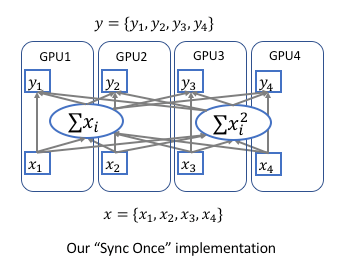
\includegraphics[width=0.7\linewidth]{img/sync-bn.png}
            \caption{Sync BN\footnotemark}
            \label{fig:sync-bn}
        \end{figure}
        \footnotetext{Source: \href{https://hangzhang.org/PyTorch-Encoding/tutorials/syncbn.html}{https://hangzhang.org/PyTorch-Encoding/tutorials/syncbn.html}}
        
        (Source: \href{https://hangzhang.org/PyTorch-Encoding/tutorials/syncbn.html}{Hang Zhang's blog})
    \end{answer}

    \item Given the following code snippet. What might be a problem with it? How would you improve it?

    \begin{lstlisting}
    import numpy as np
    
    def within_radius(a, b, radius):
        if np.linalg.norm(a - b) < radius:
            return 1
        return 0
    
    def make_mask(volume, roi, radius):
        mask = np.zeros(volume.shape)
        for x in range(volume.shape[0]):
            for y in range(volume.shape[1]):
                for z in range(volume.shape[2]):
                    mask[x, y, z] = within_radius((x, y, z), roi, radius)
        return mask
    \end{lstlisting}
    
    \begin{answer}
        The issue with the code is that it is not properly vectorized, i.e. it doesn't utilize its optimized and pre-compiled functions and operations. One way to vectorize the code is as follows:
        \begin{lstlisting}
            import numpy as np
            np.random.seed(42)
            
            m, n, r = 90, 110, 100
            volume = np.random.rand(m, n, r)
            roi = np.random.rand(3)
            radius = 3.4
            
            first = ((np.arange(m)-roi[0])**2).reshape(m, 1, 1)  # (m, 1, 1)
            second = ((np.arange(n)-roi[1])**2).reshape(1, n, 1) # (1, n, 1)
            third = ((np.arange(r)-roi[2])**2).reshape(1, 1, r)  # (1, 1, r)
            
            vals = first + second + third   # (m, n, r)
            mask = vals < radius**2         # (m, n, r)
        \end{lstlisting}
        
    \end{answer}
    
\end{QandA}

\subsection{Data Structures}
\begin{QandA}
    \item 
\end{QandA}

\section{Machine learning workflows}
\subsection{Basics}
\begin{QandA}
    \item Explain supervised, unsupervised, weakly supervised, semi-supervised, and active learning.
    \begin{answer}
        \textit{Supervised learning} is the machine learning task of learning a function that maps an input to an output based on example input-output pairs. It infers a function from labeled training data consisting of a set of training examples. (Source: \href{https://en.wikipedia.org/wiki/Supervised_learning}{Wikipedia}) \\\\
        \textit{Unsupervised learning} is the machine learning task of learning patterns from unlabeled data. The hope is that through mimicry, the algorithm is forced to build a compact internal representation of its world and then generate imaginative content from it (Source: \href{https://en.wikipedia.org/wiki/Unsupervised_learning}{Wikipedia}) \\\\
        \textit{Weakly supervised learning} is a branch of machine learning where noisy, limited, or imprecise sources are used to provide supervision signal for labeling large amounts of training data in a supervised learning setting. This approach alleviates the burden of obtaining hand-labeled data sets, which can be costly or impractical. Instead, inexpensive weak labels are employed with the understanding that they are imperfect, but can nonetheless be used to create a strong predictive model. (Source: \href{https://en.wikipedia.org/wiki/Weak_supervision}{Wikipedia}) \\\\
        \textit{Semi-supervised learning} is an approach to machine learning that combines a small amount of labeled data with a large amount of unlabeled data during training. Semi-supervised learning falls between unsupervised learning and supervised learning, and is a special instance of weak supervision. (Source: \href{https://en.wikipedia.org/wiki/Semi-supervised_learning}{Wikipedia}) \\\\
        \textit{Active learning} is a branch of machine learning where a learning algorithm can interactively query a user (or some other information source) to label new data points with the desired outputs. (Source: \href{https://en.wikipedia.org/wiki/Active_learning}{Wikipedia}) \\\\
        \textit{Self-supervised learning} is a branch of machine learning that learns from unlabeled data by automatically extracting labels from the sample. For example, we could mask out a word in a sentence, which the algorithm then has to predict. (Source: \href{https://en.wikipedia.org/wiki/Self-supervised_learning}{Wikipedia})
    \end{answer}

    \item Empirical risk minimization.
    \begin{InnerQandA}
        \item What’s the risk in empirical risk minimization? 
        \begin{answer}
            Assume that there is a joint probability distribution $P(x, y)$ over an input space $X$ and a target space $Y$. The goal is to learn a function $h: X \rightarrow Y$ (often called hypothesis) which outputs an object $y \in Y$, given $x \in X$. Moreover, assume that we are given a non-negative real-valued loss function $L(\hat{y}, y)$ which measures how different the prediction $\hat{y}$ of a hypothesis is from the true outcome $y$. \\\\
            The risk associated with the hypothesis $h(x)$ is then defined as the expectation of the loss function:
            \begin{align*}
                R(h) = \Exp{L(h(x), y)} = \int L(h(x), y) dP(x, y)
            \end{align*}
            A loss function commonly used in theory is the 0-1 loss function:
            \begin{align*}
                L(\hat{y}, y) = \begin{cases}
                    1 &\text{if } \hat{y} \neq y \\
                    0 &\text{if } \hat{y} = y
                \end{cases}
            \end{align*}
            The ultimate goal of a learning algorithm is to find a hypothesis $h^*$ among a fixed class of functions $\mathcal{H}$ for which the risk $R(h)$ is minimal:
            \begin{align*}
                h^* = \argmin_{h \in \mathcal{H}} R(h)
            \end{align*}
            (The above answer is for the general form of Risk Minimization, instead of the Empirical one. See the next answer which introduces the idea of Empirical Risk Minimization.)
        \end{answer}

        \item Why is it empirical?
        \begin{answer}
            In practice, the risk $R(h)$ cannot be computed because the distribution $P(x, y)$ is unavailable. However, we can compute an approximation, called empirical risk, by averaging the loss function on the training set:
            \begin{align*}
                R_{\text{emp}} = \frac{1}{n}\sum_{i=1}^n L(h(x_i), y_i) 
            \end{align*}
            The empirical risk minimization principle states that the learning algorithm should choose a hypothesis $\hat{h}$ which minimizes the empirical risk:
            \begin{align*}
                \hat{h} = \argmin_{h \in \mathcal{H}} R_{\text{emp}}(h)
            \end{align*}
        \end{answer}

        \item How do we minimize that risk?
        \begin{answer}
            Empirical risk minimization for a classification problem with a 0-1 loss function is known to be an NP-hard problem even for linear classifiers. \\\\
            In practice, machine learning algorithms cope with this problem by employing a convex approximation to the 0-1 (like hinge loss for SVM), which is easier to optimize.
        \end{answer}
        
        (Source: \href{https://en.wikipedia.org/wiki/Empirical_risk_minimization}{Wikipedia})
    \end{InnerQandA}

    \item Occam's razor states that when the simple explanation and complex explanation both work equally well, the simple explanation is usually correct. How do we apply this principle in ML?
    \begin{answer}
        Statistical versions of Occam's razor have a more rigorous formulation than what philosophical discussions produce. In particular, they must have a specific definition of the term simplicity, and that definition can vary. \\\\
        For example, Minimum Description Length (MDL) is a model selection principle where the shortest description of the data is the best model. Within Algorithmic Information Theory, the description length of a data sequence is defined as the length of the smallest program that outputs that data set. 
    
        (Source: \href{https://en.wikipedia.org/wiki/Minimum_description_length}{Wikipedia})
    \end{answer}

    \item What are the conditions that allowed deep learning to gain popularity in the last decade?
    \begin{answer}
        The three main factors that allowed deep learning to gain popularity are:
        \begin{itemize}
            \item Increased access to large datasets of high quality and fine-grained labels (ImageNet, CityScapes).
            \item Improved hardware (GPUs, TPUs). 
            \item Algorithmic advances (Residual Connections, Attention mechanism, BatchNorm)
        \end{itemize}
    \end{answer}

    \item If we have a wide NN and a deep NN with the same number of parameters, which one is more expressive and why?
    \begin{answer}
        Deeper networks are more expressive, since they encode an inductive bias that complex functions can be modeled as composition of simple functions. In turn, this allows the network to learn multiple levels of an abstraction hierarchy. Empirically, it has been shown that deeper networks lead to more compact models with better generalization performance. 
    \end{answer}

    \item The Universal Approximation Theorem states that a neural network with 1 hidden layer can approximate any continuous function for inputs within a specific range. Then why can’t a simple neural network reach an arbitrarily small positive error?
    \begin{answer}
        While at first look the universality of 2-layer networks is appealing, one aspect that is not explicitly stated is the arbitrarily large requirements for width. Typically, these networks require exponential width with respect to the input size, which in turn leads to an exponential increase in memory and computation time. \\\\
        Moreover, the Universal Approximation Theorem states that these wide networks can approximate the train set arbitrarily close -- but make no statements about the generalization performance on the test set. Empirically, it has been shown that networks that overfit on the train set do not generalize well on test set, since the network merely memorizes in the input-output pairs.
    \end{answer}

    \item What are saddle points and local minima? Which are thought to cause more problems for training large NNs?
    \begin{answer}
        A \textit{saddle point} is a point on the surface of the graph of a function where the slopes (derivatives) in orthogonal directions are all zero (a critical point), but which is not a local extremum of the function. \\\\
        A function $f$ has a \textit{local minimum} at $x^*$ if there exists some $\epsilon > 0$ such that $f(x^*) \le f(x)$ for all $x \in X$ within distance $\epsilon$ of $x^*$. \\\\
        Today, neither saddle points nor local minima are considered significant problems (e.g. see \href{https://arxiv.org/abs/1412.6544}{this paper}). Nevertheless, let us provide some intuitive explanations for why these long-feared mathematical phenomena are not as harmful or common.\\\\
        For a point to truly be a local minimum of the loss function, it has to be a local minimum in all directions, where each direction is specified by one of the parameters of the network. In contrast, for a saddle point, only one direction has to be different than others. Given that we usually train million- (or even billion-) parameter models, it is much more likely that at least one direction displays different behavior than the others, as opposed to all of them displaying the same behavior. Therefore, we can conclude that local minima are not as common. \\\\
        Okay, but what if we actually do arrive at a local minima, or even more commonly -- a saddle point? It is important to stress that today's networks are typically trained with Stochastic Gradient Descent (or one of its momentum-based variants), as opposed to pure Gradient Descent. Since we are calculating the loss wrt. the current batch (and not the entire dataset), we are not truly traversing the original loss landscape, but a proxy of it. And if we eventually get stuck in a local minima / saddle point in the loss landscape (or even its current proxy), in the next iteration we are optimizing over a different batch, which is a different proxy of the loss, and therefore will slightly nudge us in a different direction. This regularization effect is a huge reason why we are able to train neural networks that show remarkable capabilities. 

        (See more \href{https://blog.paperspace.com/intro-to-optimization-in-deep-learning-gradient-descent/}{here})
    \end{answer}

    \item Hyperparameters.
    \begin{InnerQandA}
        \item What are the differences between parameters and hyperparameters?
        \begin{answer}
            Parameters are quantities that are optimized by the model during the training process (e.g. weights of a neural network). \\\\
            Hyperparameters are quantities related to the learning procedure, which are not optimized during training, but are set by the user before the training starts (e.g. learning rate of the optimizer).
        \end{answer}

        \item Why is hyperparameter tuning important?
        \begin{answer}
            Each learning algorithm has unique properties. When it comes to selecting a value for a hyperparameter, in general there is no one-size-fits-all. For this reason, we need to tune the values of the hyperparemeter on a hold-out validation set. \\\\
            Furthermore, even if a given hyperparameter value seems to work well for a given model when trained on a particular dataset, there is no guarantee that the same value will be appropriate when the model is trained on a different dataset.
        \end{answer}
        \begin{figure}
            \centering
            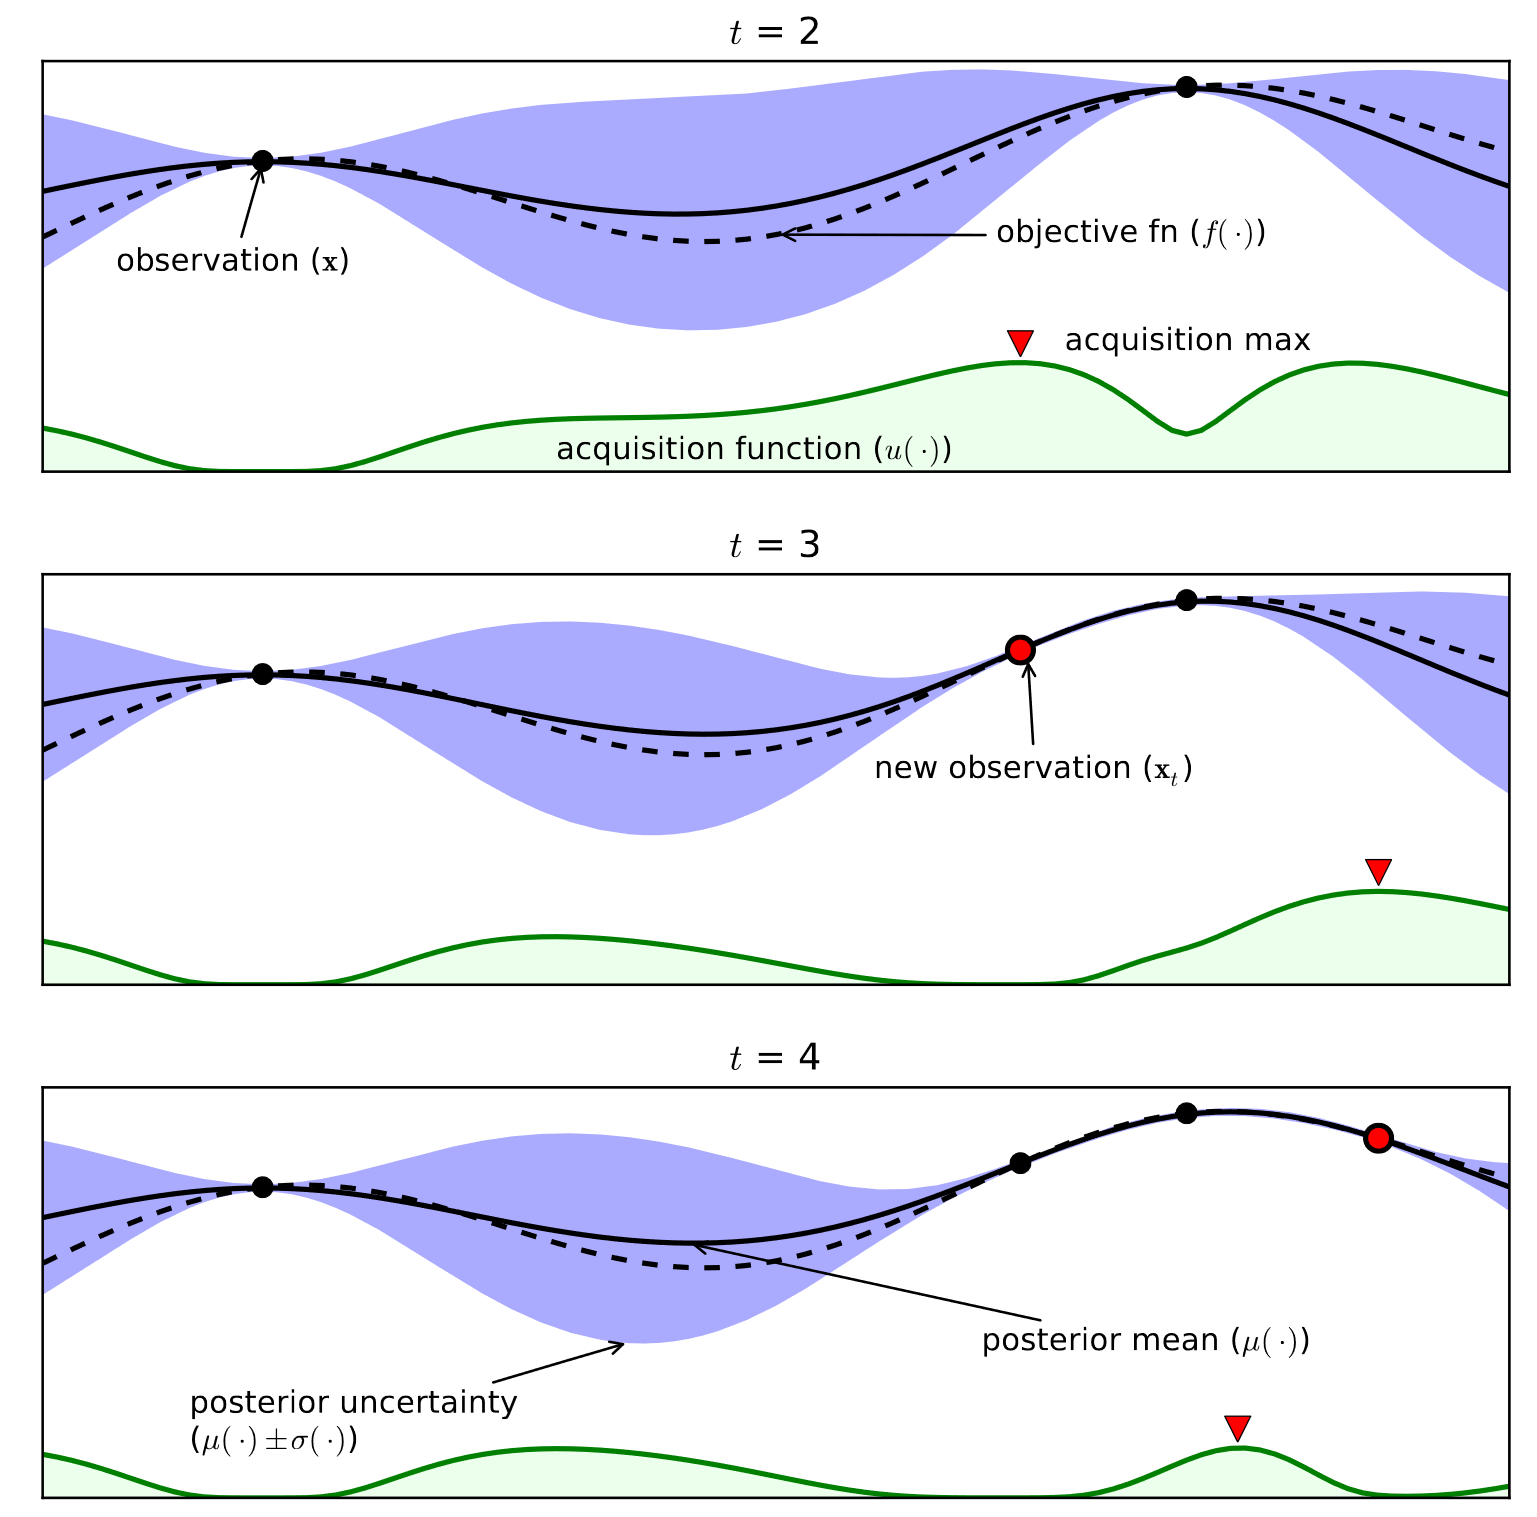
\includegraphics[width=0.7\columnwidth]{img/bo.png}
            \caption{Bayesian Optimization\footnotemark.}
            \label{fig:bo}
        \end{figure}
        \footnotetext{Source: \href{https://towardsdatascience.com/shallow-understanding-on-bayesian-optimization-324b6c1f7083}{https://towardsdatascience.com/shallow-understanding-on-bayesian-optimization-324b6c1f7083}}
        
        \item Explain an algorithm for tuning hyperparameters. 
        \begin{answer}
            Two fairly naive, but commonly used algorithms for tuning hyperparameters are:
            \begin{itemize}
                \item Grid Search -- given a set of values for each hyperparameter, the algorithm looks over each possible combination.
                \item Random Search -- given an interval of possible hyperparameter values, the algorithm trains the model by sampling randomly from the provided ranges.
            \end{itemize}
            One major drawback of these two approaches is that they are uninformative -- the choice of the next set of parameters is independent of the performance of the previous choice. This serves as a motivating factor as to why someone might consider using Bayesian Optimization. \\\\
            Suppose we are given a function $f: X \rightarrow \R$ which maps a set of hyperparameters $x \in X$ to a metric of interest (eg. accuracy). The main goal is to optimize the function and retrieve the best hyperparameters:
            \begin{align*}
                x^* = \argmax_x f(x)
            \end{align*}
            Practically speaking, this function would wrap the entire training procedure of the model, which means that we cannot apply gradient based optimization since it is not differentiable. We have to settle on optimizing the function $f$ by merely evaluating it at a given point $x$. Given these constraints, we now introduce the two main components of Bayesian Optimization: surrogate model, and acquisition function. \\\\
            Since we lack an expression for the objective function, the first step is to use a \textit{surrogate model} to approximate $f(x)$. While there are several possible approaches for the surrogate function, a common choice is to use Gaussian Processes (GPs). 
            GPs are especially useful for our purposes, since they not only provide a model which best fits the data $\mu(x)$, but also produce uncertainty estimates $\sigma(x)$ at each point $x$. \\\\
            Next, we need to choose an \textit{acquisition function}, whose main purpose is to decide which point $x$ is best to sample next, based on the information provided by the surrogate model. Given that we have already sampled several hyperparameters $x_1, x_2, \ldots$ for evaluation, the acquistion function has to make a choice whether to keep exploring in the already visited regions in order to greedily optimize the surrogate to the objective $f$, or take on a risk by venturing into a previously unexplored area which could potentially yield an even better optimum. This is known as the exploration-exploitation dilemma in Bayesian optimization. Among the several possible choices for an acquisition function, the Upper Confidence Bound (UCB) is the most intuitive one, because it explicitly trades off between exploring new regions, and exploiting already visited ones. In particular, the affinity for the hyperparameter $x$ is estimated as follows:
            \begin{align*}
                a_{\text{UCB}}(x; \lambda) = \mu(x) + \lambda \sigma(x)
            \end{align*}
            where $\mu(x)$ is the mean of the GP posterior at $x$, $\sigma(x)$ is the standard deviation of the GP posterior at $x$, and $\lambda$ is a hyperparameter which trades-off the two (this is user set, and not optimized). As we discussed, the affinity for each hyperparameter $x$ is a weighted sum of the expected performance and the uncertainty surrounding the choice of this parameter. \\\\
            See Figure \ref{fig:bo} for a visual explanation of the inter-play between the surrogate model and the acquisition function. Finally, here is what the Bayesian Optimization algorithm would look like in pseudocode:
            \begin{enumerate}[label={\arabic*.}]
                \item Evaluate $f(x)$ at $n$ initial points 
                \item While $n \le N$ repeat:
                \begin{itemize}
                    \item Update the surrogate model (the GP posterior) using all avaliable data $\mathcal{D}_{1:n}$ 
                    \item Select the next candidate: $x_{n+1} = \argmax_{x}a_{\text{UCB}}(x, \lambda)$
                    \item Evaluate $y_{n+1} = f(x_{n+1})$ 
                    \item Augment the dataset $\mathcal{D}_{1:n+1} = \{ \mathcal{D}_{1:n}, (x_{n+1}, y_{n+1}) \}$
                \end{itemize}
            \item Return the $x$ that evaluated with the largest $f(x)$
        \end{enumerate}

        

        (Source: \href{https://ekamperi.github.io/machine%20learning/2021/05/08/bayesian-optimization.html}{Stathis Kamperis's blog})
        \end{answer}
    \end{InnerQandA}

    \item Classification vs. regression.
    \begin{InnerQandA}
        \item What makes a classification problem different from a regression problem? 
        \begin{answer}
            Classification is the task of predicting a discrete class label, whereas regression is the task of predicting a continuous quantity.
        \end{answer}

        \item Can a classification problem be turned into a regression problem and vice versa?
        \begin{answer}
            While it is \href{https://machinelearningmastery.com/classification-versus-regression-in-machine-learning/}{technically possible} to turn a classification (and vice versa), there is rarely ever a reason to do so. Following are some of the reasons why this is not a good idea:
            \begin{itemize}
                \item One loses information by binning the response. 
                \item Continuous targets have an order. In general, classification problems don't assume class ordering.
                \item Continuity implies smoothness. This is in contrast to the orthogonal representation of one-hot encoded labels.
            \end{itemize}
            (Source: \href{https://stats.stackexchange.com/questions/565537/is-there-ever-a-reason-to-solve-a-regression-problem-as-a-classification-problem}{StackExchange})
        \end{answer}
    \end{InnerQandA}
    
    \item Parametric vs. non-parametric methods.
    \begin{InnerQandA}
        \item What’s the difference between parametric methods and non-parametric methods? Give an example of each method.
        \begin{answer}
            A learning model that summarizes data with a set of parameters of fixed size (independent of the number of training examples) is called a \textit{parametric model}. Some prominent examples: Linear regression, Logistic regression, Neural Networks, Naive Bayes. \\\\
            In contrast, \textit{non-parametric} methods do not take a predetermined form, but are constructed according to the information derived from the data. For this reason, they require larger sample sizes because the data must supply the model structure. Some prominent examples: k Nearest Neighbors, Decision Trees, Gaussian Processes.

            (Source: \href{https://machinelearningmastery.com/parametric-and-nonparametric-machine-learning-algorithms/}{MachineLearningMastery}, \href{https://en.wikipedia.org/wiki/Nonparametric_regression}{Wikipedia}) \\\\
            Interestingly, SVMs can be considered both parametric and non-parametric model, depending on whether you view them from the primal (parameters $w$ and $b$) or the dual problem space (formulation through support vectors). 

            (Source: \href{https://www.quora.com/Do-Support-Vector-Machines-come-under-parametric-or-non-parametric-models-and-why}{Quora})
        \end{answer}

        \item When should we use one and when should we use the other?
        \begin{answer}
            To answer this question, we will consider two aspects:
            \begin{ListAlph}
                \item \textit{Dataset size}: Non-parametric methods are more applicable in cases when we have larger datasets that provide sufficient coverage s.t. we can derive the entire model structure based on the data alone. Otherwise, if the datasets are not large enough, we can inject a prior into our training process by fixing the parametric form of the model. This allows the optimization procedure to only focus on inferring the parameter values, and not having to derive the entire model structure.

                \item \textit{Inference time requirements}: Since parametric models use a fixed parametrization, they are more applicable in cases when we need consistent inference time guarantees. In contrast, the prediction time of non-parametric methods might depend on the dataset size (e.g. finding k-nearest neighbors, iterating over all support vectors, \ldots)
            \end{ListAlph}
            
        \end{answer}
    \end{InnerQandA}
    
    \item Why does ensembling independently trained models generally improve performance?
    \begin{answer}
        Consider $K$ regression models, each of which has an error $\epsilon_k \sim N(0, \sigma)$, with $\Vari{\epsilon_k} = \Exp{\epsilon_k^2} = v$ and covariances $\Cov{\epsilon_k, \epsilon_l} = \Exp{\epsilon_k \epsilon_l} = c$ (notice that $\Exp{\epsilon_k}=0$). Then, the expected squared error of the ensemble predictor (with each model having the same weight) is given as:
        \begin{align*}
            \Exp{\left( \frac{1}{K} \sum_{k} \epsilon_k \right)^2} &= \frac{1}{K^2} \Exp{ \sum_k \left(\epsilon_k^2 + \sum_{l, l \neq k} \epsilon_k \epsilon_l \right)} \\
            &= \frac{1}{K^2} \left( \sum_{k} \Exp{\epsilon_k^2} + \sum_k \sum_{l, l \neq k} \Exp{\epsilon_k \epsilon_l} \right) \\
            &= \frac{1}{K^2} \left( Kv + K(K-1)c \right) \\
            &= \frac{1}{K}v + \frac{K-1}{K}c
        \end{align*}
        Now, consider the following two cases:
        \begin{ListAlph}
            \item The errors are maximally correlated:
            \begin{align*}
                corr(\epsilon_k, \epsilon_l) &= 1 \\
                \frac{\Cov{\epsilon_k, \epsilon_l}}{\sqrt{\Vari{\epsilon_k} \Vari{\epsilon_l}}} &= 1 \\
                (\Cov{\epsilon_k, \epsilon_l})^2 &= \Vari{\epsilon_k} \Vari{\epsilon_l} \\
                c^2 &= v \cdot v \\
                \implies c &= v
            \end{align*}

            Then, the error becomes:
            \begin{align*}
                \Exp{\left( \frac{1}{K} \sum_{k} \epsilon_k \right)^2} &= \frac{1}{K}v + \frac{K-1}{K}c \\
                &= \frac{1}{K}v + \frac{K-1}{K}v & (c = v) \\
                &= v \\ 
                &= \Exp{\epsilon_k^2}
            \end{align*}
            In other words, we observe no gain wrt. a single model when the errors of the models are correlated.
    
            \item The errors are uncorrelated:
            \begin{align*}
                corr(\epsilon_k, \epsilon_l) &= 0 \\
                \implies \Cov{\epsilon_k, \epsilon_l} &= 0 \\
                \implies c &= 0
            \end{align*}
            In this case, the error becomes:
            \begin{align*}
                \Exp{\left( \frac{1}{K} \sum_{k} \epsilon_k \right)^2} &= \frac{1}{K}v + \frac{K-1}{K}c \\
                &= \frac{1}{K}v  & (c = 0) \\
                &= \frac{\Exp{\epsilon_k^2}}{K}
            \end{align*}
            In contrast to before, we notice a $K$-fold reduction in the error wrt. a single model.
        \end{ListAlph}
        
    \end{answer}
    
    \item Why does L1 regularization tend to lead to sparsity while L2 regularization pushes weights closer to 0?
    \begin{answer}
        The reason is because $L_1(w) = \vert w \vert$ converges slower to $0$ when $w \rightarrow 0$, compared to  $L_2(w)=w^2$. Therefore, when minimizing the L1 loss, the optimizer has to really push the magnitude of the weights close to $0$ in order to achieve regularization loss close to $0$. \\\\
        Let $w = 0.001$. Then, $L_1(w) = \vert 0.001 \vert = 0.001$, but $L_2(w) = (0.001)^2 = 0.000001$. We see that for the same value of $w$, the L2 term is much lower than the L1 term. As a consequence, in order to minimize the L1 regularization loss, the optimizer is forced to push $w$ even closer to $0$.
    \end{answer}
    
    \item Why does an ML model’s performance degrade in production?
    \begin{answer}
        Sources of bugs in production can be:
        \begin{ListAlph}
            \item Caused by the training data:
            \begin{itemize}
                \item Selection bias: the sampling procedure for collecting the dataset does not account for all relevant characteristics of the population. 
                \item Missing data: the decision on how to handle missing data (by dropping it, or imputing it with a certain technique) might not hold beyond the offline test set evaluation.
                \item Misspecified schema: the data is there, but the semantics of the features can be misunderstood. This happens when there is no proper documentation (schema) explaining how the dataset was gathered, and what the features exactly mean.
            \end{itemize}
            
            \item Caused by the model:
            \begin{itemize}
                \item Model mismatch: the model assumes structure not applicable to the data seen in deployment.
            \end{itemize}

            \item Caused by the algorithm:
            \begin{itemize}
                \item Classic implementation bugs: off-by-one, type mismatches, value-v-reference, etc.
                \item Subtle mathematical bugs: incorrect gradients, unexpected broadcast, biased estimators, etc.
                \item Fundamental mathematical challenges: non-convex optimization, numerical stability, sampling noise, etc.
            \end{itemize}

            \item Caused by the test data. Given a distribution $P(X, Y)$, where $X$ are the inputs, and $Y$ are the targets, a model deployed in production can experience the following shifts in data:
            \begin{itemize}
                \item Covariate shift: $P(X)$ changes, but $P(Y \g X)$ remains the same.
                \item Label shift: $P(Y)$ changes, but $P(X \g Y)$ remains the same.
                \item Concept drift: $P(Y \g X) $ changes, but $P(X)$ remains the same.
            \end{itemize}
        \end{ListAlph}
        (See more \href{https://huyenchip.com/2022/02/07/data-distribution-shifts-and-monitoring.html}{here})
    \end{answer}
    
    \item What problems might we run into when deploying large machine learning models?
    \begin{answer}
        There are several challenges that come with deploying large ML models:
        \begin{ListAlph}
            \item \textit{Component efficiency}. For complex models with many different components, it's especially important to conduct ablation studies -- removing each component while keeping the rest -- to determine the efficiency of each component. One might consider discarding / substituting components that are inefficient in time or provide only minor improvement in accuracy.

            \item \textit{Server- vs client- side inference}. Inferencing on the user phone consumes the phone's memory and battery, and makes it harder for collecting user feedback. Inferencing on the cloud increases the product latency, requires setting up a server to process all user requests, and might scare away privacy-conscious users.

            \item \textit{Interpretability}. If a model predicts that someone shouldn't get a loan, that person deserves to know the reason why. One needs to consider the performance/interpretability tradeoffs. Making a model more complex might increase its performance but make the results harder to interpret. 

            \item \textit{Bias}. One should do extensive testing and model validation to confirm that the model doesn't perpetuate potential biases that can occur in the training data, such as racial and gender stereotypes. Moreover, it's important to design post-hoc safety systems that prevent users with malicious intents.
        \end{ListAlph}

        (Source: \href{https://huyenchip.com/machine-learning-systems-design/design-a-machine-learning-system.html#serving-091rIYw}{Chip Huyen's ML system design interview booklet})
    \end{answer}

    
    \item Your model performs really well on the test set but poorly in production.
    \begin{InnerQandA}
        \item What are your hypotheses about the causes?
        \begin{answer}
            As we discussed above, the three main reasons for change in performance compared to the test set could be attributed to one or more of the following: covariate shift, label shift, concept drift. Let us explain each one in a bit more detail.
            
            \begin{ListAlph}

            \item During \textit{covariate} shift $P(X)$ changes, but $P(Y \g X)$ remains the same. In supervised ML, the label is the variable of direct interest, and the input features are covariate variables. \\

            Suppose you want to build a model that predicts breast cancer. Research has shown that the risk of breast cancer is higher for women over the age of 40, so you decide to have a variable “age” as your input. Given that women over 40 are more likely to have breast cancer,  due to potentially sampling bias from the hospital data, during training we might have more women with age over 40 compared to inference time — resulting in $P(X)$ changing. However, the probability of a patient of a certain age having cancer doesn't change just because we start seeing a higher number of young users -- therefore, $P(Y \g X)$ remains the same. The change in our user base doesn't affect the nature of the cancer. \\
        
            \item During \textit{label shift} $P(Y)$ changes, but $P(X \g Y)$ remains the same.  \\\\
            Quite often, label shift is accompanied with covariate shift. Consider the breast cancer example again, and suppose we have covariate shift ($P(X)$ changes but $P(Y \g X)$ remains the same). Because of the change in P(X), we are also bound to see a change in class distribution: during training there are more positive classes (due to the aforementioned sampling bias in our dataset), but during inference time there are less patients with positive classes (since we experience change in user base, more women with age less than 40 start using the model, but we also know they are less likely to have cancer) — therefore $P(Y)$ also changes. However, the distribution of age for sick patients doesn't change just because we start seeing  lower number of users who have cancer -- therefore, $P(X \g Y)$ remains the same. Again, the change in our user base doesn't affect the nature of the cancer. \\
            
            However, it’s not always the case that label shift is accompanied by covariate shift. Imagine that there is now a preventive drug that every woman takes that helps reduce their chance of getting breast cancer. The probability $P(Y \g X)$ reduces for women of all ages, so it’s no longer a case of covariate shift. However, given a person with breast cancer, the age distribution remains the same so this is still a case of label shift.\\
            
            \item During \textit{concept} drift $P(Y \g X)$ changes, but $P(X)$ remains the same. You can think of this as “same input, different output”. \\\\
            Consider you’re in charge of a model that predicts the price of a house based on its features. Before COVID-19, a 3 bedroom apartment in San Francisco could cost \$2,000,000. However, at the beginning of COVID-19, many people left San Francisco, so the same house would cost only \$1,500,000. So even though the distribution of house features remains the same, the conditional distribution of the price of a house given its features has changed.\\\\
            In many cases, concept drifts are cyclic or seasonal. For example, rideshare’s prices will fluctuate on weekdays versus weekends, and flight tickets rise during holiday seasons. Companies might have different models to deal with cyclic and seasonal drifts. For example, they might have one model to predict rideshare prices on weekdays and another model for weekends.
            
            \end{ListAlph}
        \end{answer}

        \item How do you validate whether your hypotheses are correct?
        \begin{answer}
            In order to validate whether our hypotheses are correct, we need to put methods in place that are able to detect these data distribution shifts. One can classify the approaches in two primary groups: statistical methods, and time scale windows for detecting shifts.\\\\
            \textit{Statistical methods} aim to detect a shift between the training and serving data by quantifying it in some statistical sense. One simple approach is to compare the moments (mean, variance, skewness, kurtosis, etc.) of the two distributions -- in case these quantities significantly differ, one can conclude that we there is a shift. However, if there is no significant difference between the quantities describing the two distributions, we cannot conclude that there is no shift present, since these statistics are not sufficient. \\\\
            A more sophisticated solution is to use a two-sample hypothesis test, shortened as two-sample test. It’s a test to determine whether the difference between two populations (two sets of data) is statistically significant. If the difference is statistically significant, then the probability that the difference is a random fluctuation due to sampling variability is very low, and therefore, the difference is caused by the fact that these two populations come from two distinct distributions. If you consider the data from yesterday to be the source population and the data from today to be the target population and they are statistically different, it’s likely that the underlying data distribution has shifted between yesterday and today. Some examples include: Kolmogorov-Smirnov test (non-parametric test, but can only be used for one-dimensional data), Least-Squares Density Difference (based on the least squares density-difference estimation method), Maximum Mean Discrepancy (a kernel-based technique for multivariate two-sample testing), and many more. \\\\
            On the other hand, \textit{time scale windows} are designed to detect temporal shifts that happen over time. To detect temporal shifts, a common approach is to treat input data to ML applications as time series data. \\\\
            When dealing with temporal shifts, the time scale window of the data we look at affects the shifts we can detect. If your data has a weekly cycle, then a time scale of less than a week won’t detect the cycle. Therefore, by setting the time window too small, your detection technique can produce a false alarm simply due to the seasonality inherent to the data. \\\\
            When computing running statistics over time, it’s important to differentiate between cumulative and sliding statistics. Sliding statistics are computed within a single time scale window, e.g. an hour. Cumulative statistics are continually updated with more data. This means for each beginning of a time scale window, the sliding accuracy is reset, whereas the cumulative sliding accuracy is not. Because cumulative statistics contain information from previous time windows, they might obscure what happens in a specific time window. 
        \end{answer}

        \item Imagine your hypotheses about the causes are correct. What would you do to address them?
        \begin{answer}
            To make a model work with a new distribution in production, there are three main approaches. The first is the approach that currently dominates research: train models using massive datasets. The hope here is that if the training dataset is large enough, the model will be able to learn such a comprehensive distribution that whatever data points the model will encounter in production will likely come from this distribution. \\\\
            The second approach, less popular in research, is to adapt a trained model to a target distribution without requiring new labels. \href{http://proceedings.mlr.press/v28/zhang13d.pdf}{Zhang et al. (2013)} used causal interpretations together with kernel embedding of conditional and marginal distributions to correct models’ predictions for both covariate shifts and label shifts without using labels from the target distribution. Similarly, \href{http://proceedings.mlr.press/v97/zhao19a.html}{Zhao et al. (2020)} proposed domain-invariant representation learning: an unsupervised domain adaptation technique that can learn data representations invariant to changing distributions. However, this area of research is heavily underexplored and hasn’t found wide adoption in industry. \\\\
            The third approach is what is usually done in the industry today: retrain your model using the labeled data from the target distribution. However, retraining your model is not so straightforward. Retraining can mean retraining your model from scratch on both the old and new data or continuing training the existing model on new data. The latter approach is also called fine-tuning.
        \end{answer}

    (Source: \href{https://huyenchip.com/2022/02/07/data-distribution-shifts-and-monitoring.html}{Chip Huyen's blog on Data Distribution Shifts})
    \end{InnerQandA}
\end{QandA}

\subsection{Sampling and creating training data}
\begin{QandA}
    \item If you have 6 shirts and 4 pairs of pants, how many ways are there to choose 2 shirts and 1 pair of pants?
    \begin{answer}
        \begin{align*}
            {6 \choose 2} \cdot {4 \choose 1} = 15 \cdot 4 = 60
        \end{align*}
    \end{answer}

    \item What is the difference between sampling with vs. without replacement? Name an example of when you would use one rather than the other?
    \begin{answer}
        When we sample \textit{with replacement}, the two sample values are independent. Practically, this means that what we get on the first one doesn't affect what we get on the second. Mathematically, this means that the covariance between the two is zero. \\\\
        In sampling \textit{without replacement}, the two sample values aren't independent. Practically, this means that what we get on the first one affects what we can get for the second one. Mathematically, this means that the covariance between the two isn't zero. That complicates the computations. In particular, if we have a SRS (simple random sample) without replacement, from a population with variance $\sigma^2$, then the covariance of two of the different sample values is $-\frac{\sigma^2}{N-1}$, where $N$ is the population size. \\\\
        With that said, if our sampling specification states that there should be no duplicates, we should sample without replacement -- keeping in mind that this in fact introduces covariance between the samples. However, if the learning algorithm has strong IID assumptions (independent and identically distributed), then we have to sample with replacement. \\\\
        Nevertheless, this argument is mostly regarding small population sizes. In large populations, if we sample without replacement, the covariance will be close to $0$ because of the $N-1$ term in the denominator. In this case, both sampling with and without replacement is nearly identical. 

        (Source: \href{https://web.ma.utexas.edu/users/parker/sampling/repl.htm}{University of Texas})
    \end{answer}

    \item Explain Markov chain Monte Carlo sampling.
    \begin{answer}
        Integration is the core computation of probabilistic inference. As a general formulation, we might want to estimate:
        \begin{align*}
            \phi = \int f(x) p(x) dx = \mathbb{E}_{p(x)} \left[ f(x) \right]
        \end{align*}
        Given independent samples $x_1, \ldots, x_n$ from $p(x)$, the estimator:
        \begin{align*}
            \hat{\phi} = \frac{1}{n} \sum_{i=1}^n f(x_i)
        \end{align*}
        is an unbiased estimator of $\phi$, meaning:
        \begin{align*}
            \mathbb{E}_{x_1, \ldots, x_n} \left[ \hat{\phi} \right] &= \mathbb{E}_{x_1, \ldots, x_n} \left[ \frac{1}{n} \sum_{i=1}^n f(x_i) \right] \\
            &= \frac{1}{n} \sum_{i=1}^n \Exp{f(x_i)} \\
            &= \frac{1}{n} (n \cdot \phi) \\
            &= \phi
        \end{align*}
        Algorithms that compute expectations in the above way, by using samples $x_i \sim p(x)$, are called \textit{Monte Carlo} methods. \\\\
        A joint distribution $p(X)$ over a sequence of random variables $X = \left[ x_1, \ldots, x_n \right]$ is said to have the \textit{Markov property} if:
        \begin{align*}
            p(x_i \g x_1, x_2, \ldots, x_{i-1}) = p(x_i \g x_{i-1})
        \end{align*}
        The sequence is then called a \textit{Markov chain}. \\\\
        The main idea behind \textit{Markov Chain Monte Carlo} (MCMC) methods is to generate samples of a target distribution $p(x)$ by iteratively building approximations $q(x)$ that only need to be good locally. To illustrate the intuition behind MCMC, consider the following iterative algorithm for finding the maximum of $p(x)$:
        \begin{itemize}
            \item Draw a proposal $x' \sim q(x' \g x_t)$
            \item Compute $a = \frac{p(x')}{p(x_t)}$
            \item If $a > 1$, accept $x_{t+1} = x'$, else reject $x'$ and set $x_{t+1} = x_t$.
        \end{itemize}
        By forcing each new entry $x_{t+1}$ to be be at least as high as the previous one, we eventually reach a (local) maximum of $p(x)$. \\\\
        This very same procedure can be adapted to return a sample from $p(x)$ instead by tweaking the rules of transition from $x_t$ to $x_{t+1}$, leading to the \textit{Metropolis-Hasting} method:
        \begin{itemize}
            \item Draw a proposal $x' \sim q(x' \g x_t)$ from a proposal distribution $q$, for example $q(x' \g x_t) = N(x'; x_t, \sigma^2)$.
            \item Compute $a = \frac{p(x')}{p(x_t)} \frac{q(x_t \g x')}{q(x' \g x_t)}$.
            \item If $a > 1$, accept $x_{t+1} = x'$.
            \item Otherwise, accept with probability $a$, and reject with probability $1-a$. The outcome can be decided by drawing uniformly from $[0, 1]$ and comparing it to $a$.
        \end{itemize}
        The Markov chain stays at the same place for one time period when rejecting, meaning that the corresponding point will later show up at least 2 times. Usually, the proposal distribution is symmetric, such that $q(x_t \g x') = q (x' \g x_t)$. \\\\
        Using this method, the samples will spend more ``time'' in regions where $p(x)$ is high (lower probability of sampling a better proposition) and less ``time'' in regions where $p(x)$ is low (any proposition would be better than the current one), but the algorithm can still visit regions of low probability.
    \end{answer}

    \item If you need to sample from high-dimensional data, which sampling method would you choose?
    \begin{answer}
        Gibbs Sampling is a special case of the Metropolis-Hasting algorithm. It employs the idea that sampling from a high-dimensional joint distribution is often difficult, while sampling from a one-dimensional conditional distribution is easier. So, instead of directly sampling from the joint $p(x)$, the Gibbs sampler alternates between drawing from the respective conditional distributions, as illustrated in Algorithm \ref{alg:gibbs}.

        \RestyleAlgo{ruled}
        \begin{algorithm}
        \caption{Gibbs Sampling}\label{alg:gibbs}
            \For{$t \gets 1$ to T}{
                $x_{1}^{(t+1)} \propto p(x_1 \g x_2^{(t)}, x_3^{(t)}, \ldots, x_m^{(t)})$ \\
                $x_{2}^{(t+1)} \propto p(x_2 \g x_1^{(t+1)}, x_3^{(t)}, \ldots, x_m^{(t)})$ \\
                \vdots
                $x_{m}^{(t+1)} \propto p(x_m \g x_1^{(t+1)}, x_2^{(t+1)}, \ldots, x_{m-1}^{(t+1)})$
            }
        \end{algorithm}

        It generates an instance from the distribution of each variable in turn, conditioning it on the current values of the other variables. Thus, Gibbs is useful when drawing from the joint is hard / infeasible, while drawing from the conditional is more tractable. Although there are theoretical guarantees for the convergence of Gibbs Sampling, as it is a special case of the Metropolis-Hastings, it is unknown how many iterations are needed to reach the stationary distribution.
    \end{answer}

    \item Suppose we have a classification task with many classes. An example is when you have to predict the next word in a sentence -- the next word can be one of many, many possible words. If we have to calculate the probabilities for all classes, it’ll be prohibitively expensive. Instead, we can calculate the probabilities for a small set of candidate classes. This method is called candidate sampling. Name and explain some of the candidate sampling algorithms.
    \begin{answer}
        There exist several methods for candidate sampling:
        \begin{ListAlph}
            \item \textit{Sampled Softmax.} Assume that we have a single-label problem. Each training example $(x_i, t_i)$ consists of a context and a target class. We write $P(y \g x)$ for the probability of the target class being $y$, given that the context is $x$. \\\\
            We would like to train a function $F(x, y)$ to produce log-probabilities (commonly used in many loss functions):
            \begin{align*}
                F(x, y) = \log (P(y \g x)) + K(x)
            \end{align*}
            where $K(x)$ is an arbitrary function that doesn't depend on $y$. In full softmax training, for every training example $(x_i, t_i)$ we would need to compute $F(x_i, y)$ for all classes $y \in L$. This can get expensive if the universe of classes $L$ is very large. \\\\
            In Sampled Softmax, for each training example $(x_i, t_i)$, we pick a small set $S_i \subset L$ of "sampled" classes according to a chosen sampling function $Q(y \g x)$. Each class $y \in L$ is included in $S_i$ independently with probability $Q(y \g x_i)$:
            \begin{align*}
                P(S_i = S \g x_i) = \prod_{y \in S} Q(y \g x_i) \prod_{y \in (L - S)} (1 - Q(y \g x_i))
            \end{align*}
            We create a set of candidates $C_i$ as the union of the target class and the sampled classes:
            \begin{align*}
                C_i = S_i \cup \{ t_i \}
            \end{align*}
            Our task during training is now simplified to finding out which of the classes in $C_i$ is the target class.\\\\
            For each class $y \in C_i$, we want to compute the posterior probability that $y$ is the target class given our knowledge of $x_i$ and $C_i$, that is $P(t_i = y \g x_i, C_i)$. Now, let us further expand this term:
            \begin{align*}
                P(t_i = y \g x_i, C_i) &= \frac{P(t_i = y, x_i, C_i)}{P(C_i, x_i)} \\
                &= \frac{P(t_i = y, C_i \g x_i) P(x_i)}{P(C_i \g x_i) P(x_i)} \\
                &= \frac{P(t_i = y, C_i \g x_i)}{P(C_i \g x_i)} \\
                &= \frac{P(C_i \g t_i = y, x_i) P(t_i = y \g x_i)}{P(C_i \g x_i)} \\
                &= \frac{P(C_i \g t_i = y, x_i) P(y \g x_i)}{P(C_i \g x_i)} \\
                &= \frac{\displaystyle \prod_{y' \in C_i - \{y\}} Q(y' \g x_i) \prod_{y' \in L - C_i} (1 - Q(y' \g x_i)) P(y \g x_i) }{P(C_i \g x_i)} \\
                &= \frac{P(y \g x_i)}{Q(y \g x_i)} \frac{\displaystyle \prod_{y' \in C_i } Q(y' \g x_i) \prod_{y' \in L - C_i} (1 - Q(y' \g x_i)) }{P(C_i \g x_i)} \\
                &= \frac{P(y \g x_i)}{Q(y \g x_i)} \cdot \underbrace{K(x_i, C_i)}_{\text{const. wrt. } y_i}
            \end{align*} 
            Therefore, for the log-probs we get:
            \begin{align*}
                \log (P(t_y = y \g x_i, C_i)) \propto \log (P(y \g x_i)) - \log (Q(y \g x_i)) 
            \end{align*}
            Using this quantity, we can train our sampled version of the softmax classifier to predict which is the true class among the candidates in $C_i$. In particular, for the set of candidate classes $y \in C_i$, we compute $F(x, y)$ (output of our network), and subtract $\log Q(y \g x)$ (which is user set, and hopefully has analytical form). Then, we pass this quantity to the Cross Entropy loss function, and backpropagate in order to optimize $F$ to give us the desired outputs. \\\\
            It should be noted that the procedure of sampling the softmax is only applied during training (in order to decrease the computational complexity), whereas during inference time we compute the standard softmax.

            \item \textit{Noise Contrastive Estimation.} The idea is similar as before -- computing the entire softmax can be prohibitively expensive during training, therefore instead of comparing the true class to all other classes, we compare to a much smaller sample of negative classes. The difference is that now the target can be a (multi-)set, compared to only being a single label as before.\\\\
            Assume that each training example $(x_i, T_i) \sim P(x, T)$ consists of a context and a set of target classes. For each such example, we create sample a set of negative classes $S_i$ by sampling from a predefined distribution $Q(y \g x_i)$. \\\\
            Then, we construct a (multi-)set of candidates consisting of the sum of the target and sampled classes:
            \begin{align*}
                C_i = T_i + S_i
            \end{align*}
            \href{https://math.stackexchange.com/a/4183626}{Remember} that the logit of a Logistic Regression model in fact represents the log-odds that the input comes from the positive vs the negative class:
            \begin{align*}
                \text{logit} = \theta^T x = \log \left(\frac{P}{Q} \right) = \log(P) - \log(Q)
            \end{align*}
            For NCE, we want to output logits which represent the log-odds that the inputs come from the target set $T$ (true distribution $P$), instead of the sampled set $S$ (the noise distribution $Q$). \\\\
            For this reason, we "repurpose" our network to output $F(x, y) := \log(P(y \g x))$, and subtract from it $\log(Q(y \g x))$:
            \begin{align*}
                z(x, y) := F(x, y) - \log(Q(y \g x)) = \log(P(y \g x)) - \log(Q(y \g x))
            \end{align*}
            resulting in the desired set of logits, which as mentioned above, represent the log-odds that the input comes from the target set $T$ vs the sampled set $S$. It should be noted that the $Q$ is chosen by the user, typically in such a way that its log has an analytical form. \\\\
            Finally, we pass these new logits to the Binary Cross Entropy loss function, with a label indicating whether $y$ came from $T$ or $S$. The backpropagation signal trains $F(x, y)$ to approximate what we want it to.

            \item \textit{Negative Sampling.} 
            Negative sampling is a simplified variant of Noise Contrastive Estimation where we neglect to subtract off $\log(Q(y \g x))$ during training. As a result, $F(x, y)$ is trained to approximate $ \log(P(y \g x)) - \log(Q(y \g x))$.\\\\
            It is noteworthy that in Negative Sampling, we are optimizing $F(x, y)$ to approximate something that depends on the sampling distribution $Q$. This will make the results highly dependent on the choice of sampling distribution, which is not true for the previous algorithms. 
            
            (Source: \href{https://www.tensorflow.org/extras/candidate_sampling.pdf}{Tensorflow})
        \end{ListAlph}
    \end{answer}

    \item Suppose you want to build a model to classify whether a Reddit comment violates the website’s rule. You have 10 million unlabeled comments from 10K users over the last 24 months and you want to label 100K of them.
    \begin{InnerQandA}
        \item How would you sample 100K comments to label?
        \begin{answer}
            Before we start sampling, we state a hypothesis that comments violating the website's rule over the past 24 months vary highly, and is to a high degree dependent on the predominant world events happening at the time (e.g. election campaigns, the pandemic, social movements, etc.). \\\\
            Therefore, in order to build a robust classifier capable of generalizing to unseen comments (and events related to them) in the future, we find it important to have representative samples from each historical period. \\\\
            One such approach that ensures the above-mentioned property is \textit{stratified sampling}. In particular, we select each month to represent a single strata, and then sample randomly within this population.
        \end{answer}

        \item Suppose you get back 100K labeled comments from 20 annotators and you want to look at some labels to estimate the quality of the labels. How many labels would you look at? How would you sample them?
        \begin{answer}
            Given that we have 20 annotators labeling 100K comments, in order to estimate the quality, we could look at 5\% of the comments (5000 out of the 100K), or roughly one annotator's workload. \\\\
            Since we are only interested in estimating the overall quality of the sample, we could perform \textit{simple random sampling}. On the other hand, if we were interested in the quality of work of each annotator, we could again perform stratified sampling, where each annotator's labeled pool of comments is considered a strata. From there, we can make a more informed decision about which annotators to retain in order to improve the overall quality of the work.
        \end{answer}
    \end{InnerQandA}    

    \item Suppose you work for a news site that historically has translated only 1\% of all its articles. Your coworker argues that we should translate more articles into Chinese because translations help with the readership. On average, your translated articles have twice as many views as your non-translated articles. What might be wrong with this argument? (Hint: think about selection bias.)
    \begin{answer}
        \textit{Selection bias} is the bias introduced by the selection of individuals, groups, or data for analysis in such a way that proper randomization is not achieved, thereby failing to ensure that the sample obtained is representative of the population intended to be analyzed. \\\\
        It might be the case that the 1\% of translated articles are not a random sample from the population of all articles, but only ones containing news appealing to readers in China. \\\\
        Therefore, if the news site starts putting in more resources in translating articles from the entire population (meaning not only ones that could be considered of interest to Chinese readers), the return of investment might actually not pay off, since not all articles might be of interest to the readers in China.
    \end{answer}

    \item How to determine whether two sets of samples (e.g. train and test splits) come from the same distribution?
    \begin{answer}
        The \textit{Kolmogorov–Smirnov test} (K-S test or KS test) is a nonparametric test of the equality of continuous one-dimensional probability distributions that can be used to compare a sample with a reference probability distribution (one-sample K–S test), or to compare two samples (two-sample K–S test). In essence, the test answers the question "What is the probability that this collection of samples could have been drawn from that probability distribution?" or, in the second case, "What is the probability that these two sets of samples were drawn from the same (but unknown) probability distribution?". \\\\
        The Kolmogorov–Smirnov statistic quantifies a distance between the empirical distribution function of the sample and the cumulative distribution function of the reference distribution, or between the empirical distribution functions of two samples. The null distribution of this statistic is calculated under the null hypothesis that the sample is drawn from the reference distribution (in the one-sample case) or that the samples are drawn from the same distribution (in the two-sample case). \\\\
        In order to determine whether two sets of samples come from the same distribution, the Kolmogorov statistic is computed as:
        \begin{align*}
            D_{n, m} = \sup_x \left \vert F_{1,n}(x) - F_{2, m}(x)  \right \vert
        \end{align*}
        where $F_{1, n}$ and $F_{2, m}$ are the empirical distribution functions of the first and the second sample respectively, and $\sup$ is the supremum function (see Figure \ref{fig:ks}).\\\\
        For large samples, the null hypothesis is rejected at level $\alpha$ if:
        \begin{align*}
            D_{n, m} > c(\alpha) \sqrt{\frac{n + m}{n \cdot m}}
        \end{align*}
        where $n$ and $m$ are the sizes of the first and second sample respectively. The value of $c(\alpha)$ is given in the table below for the most common levels of $\alpha$:
        \begin{table}[htb!]
        \centering
        \begin{tabular}{|c|c|c|c|}
        \hline
        \textbf{$\alpha$}    & 0.10  & 0.05  & 0.01  \\ \hline
        \textbf{$c(\alpha)$} & 1.224 & 1.358 & 1.628 \\ \hline
        \end{tabular}
        \end{table}

        It should be noted that the K-S test is only applicable to one-dimensional data. There exist other approaches, such as Least-Squares Density Difference (based on the least squares density-difference estimation method), Maximum Mean Discrepancy (a kernel-based technique for multivariate two-sample testing), and many more.
        
        \begin{figure}[htb!]
            \centering
            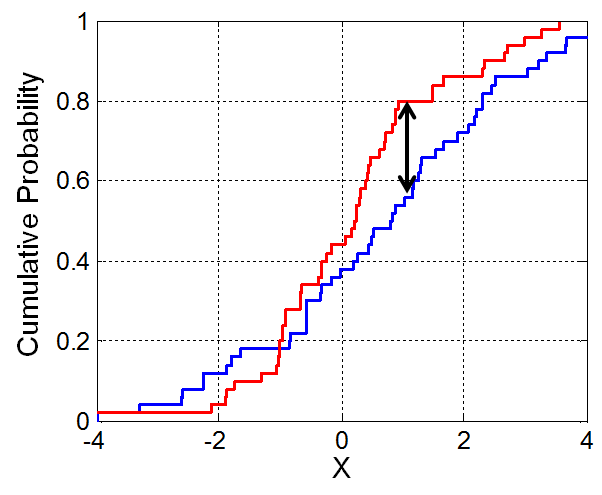
\includegraphics[width=0.4\columnwidth]{img/ks.png}
            \caption{Illustration of the two-sample Kolmogorov–Smirnov statistic. Red and blue lines each correspond to an empirical distribution function, and the black arrow is the two-sample KS statistic.}
            \label{fig:ks}
        \end{figure}
        (Source: \href{https://en.wikipedia.org/wiki/Kolmogorov%E2%80%93Smirnov_test}{Wikipedia})
    \end{answer}

    \item How do you know you’ve collected enough samples to train your ML model?
    \begin{answer}
        In statistical learning theory, the \textit{sample complexity} of a machine learning algorithm represents the training-samples that it needs in order to successfully learn a target function. \\\\
        More precisely, the sample complexity is the number of training-samples that we need to supply to the algorithm, so that the function returned by the algorithm is within an arbitrarily small error of the best possible function, with probability arbitrarily close to 1. \\\\
        There are two variants of sample complexity:
        \begin{itemize}
            \item The weak variant fixes a particular input-output distribution;
            \item The strong variant takes the worst-case sample complexity over all input-output distributions.
        \end{itemize}
        The No free lunch theorem proves that, in general, the strong sample complexity is infinite, i.e. that there is no algorithm that can learn the globally-optimal target function using a finite number of training samples. \\\\
        However, if we are only interested in a particular class of target functions (e.g, only linear functions) then the sample complexity is finite, and it depends linearly on the VC dimension on the class of target functions. \\\\
        The \textit{Vapnik–Chervonenkis} (VC) dimension is a measure of the capacity (complexity, expressive power, richness, or flexibility) of a set of functions that can be learned by a statistical binary classification algorithm. It is defined as the cardinality of the largest set of points that the algorithm can shatter, which means the algorithm can always learn a perfect classifier for any labeling of at least one configuration of those data points. \\\\
        Nevertheless, in practice these theoretical bounds are rarely used or computed. A recent \href{https://www.researchgate.net/publication/335779941_Sample-Size_Determination_Methodologies_for_Machine_Learning_in_Medical_Imaging_Research_A_Systematic_Review}{review article} suggests that the most prominent approach for sample size determination is the \textit{post hoc} method of fitting a learning curve. In essence, you take increasingly large subsets of the data, train the model, and obtain the metric of interest (e.g. accuracy). From there, plot a function with the $x$ axis being the sample size and the $y$ axis being the obtained accuracy, and then fit an exponential curve. The resulting curve should approximate the needed number of samples in order to achieve the desired accuracy (see Figure \ref{fig:sample_size}).

        (Source: \href{https://en.wikipedia.org/wiki/Sample_complexity#Sample-complexity_bounds}{Wikipedia}, \href{https://sites.uab.edu/periop-datascience/2021/06/28/sample-size-in-machine-learning-and-artificial-intelligence/}{University of Alabama at Birmingham})
    \end{answer}

    \begin{figure}[htb!]
        \centering
        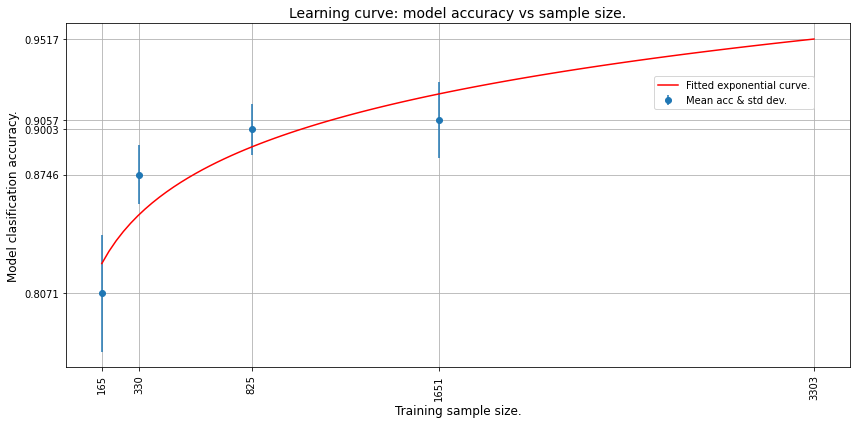
\includegraphics[width=0.9\columnwidth]{img/sample_size.png}
        \caption{Example of estimated sample size vs accuracy curve. \footnotemark }
        \label{fig:sample_size}
    \end{figure}

    \footnotetext{Source: \href{https://keras.io/examples/keras_recipes/sample_size_estimate/}{https://keras.io/examples/keras\_recipes/sample\_size\_estimate/}}

    \item How to determine outliers in your data samples? What to do with them?
    \begin{answer}
        In data analysis, anomaly detection (also referred to as outlier detection and sometimes as novelty detection) is generally understood to be the identification of rare items, events or observations which deviate significantly from the majority of the data and do not conform to a well defined notion of normal behaviour. Such examples may arouse suspicions of being generated by a different mechanism, or appear inconsistent with the remainder of that set of data. \\\\
        Anomaly detection finds application in many domains including cyber security, medicine, machine vision, statistics, neuroscience, law enforcement and financial fraud to name only a few. Anomalies were initially searched for clear rejection or omission from the data to aid statistical analysis, for example to compute the mean or standard deviation. They were also removed to better predictions from models such as linear regression, and more recently their removal aids the performance of machine learning algorithms. However, in many applications anomalies themselves are of interest and are the observations most desirous in the entire data set, which need to be identified and separated from noise or irrelevant outliers. \\\\
        There are three broad categories of anomaly detection: supervised, semi-supervised and unsupervised. Due to its wider and relevant applications, unsupervised anomaly detection is the most popular approach. \\\\
        Many anomaly detection techniques have been proposed in the literature, some of which are:
        \begin{itemize}
            \item \textit{Statistical}. A common approach is to assume Normality of the data and calculate the Z-score. Then, given a certain threshold (e.g. 3), mark all samples above the threshold as outliers; in this example, we essentially label points that are 3 standard deviations away from the mean as anomalies. 
            \item \textit{Density-based techniques}. A prominent example is to use k-NN in such a way that for each point one computes the sum of the distances of the k nearest neighbors, denoted as weight. Then, outliers are points that have the largest weight. 
            \item \textit{Gausan Anomaly Detection (\href{https://ieeexplore.ieee.org/document/9493210}{Rippel et al.})}. Use a pre-trained model as a feature extractor, and estimate the empirical mean and covariance using the dataset at hand. Then, score each item in the dataset via the Mahalanobis distance, and define a cut-off threshold. 
        \end{itemize}
        (Source: \href{https://en.wikipedia.org/wiki/Anomaly_detection}{Wikipedia})
    \end{answer}

    \item Sample duplication.
    \begin{InnerQandA}
        \item When should you remove duplicate training samples? When shouldn’t you?
        \begin{answer}
            While training a supervised learning algorithm, the usual assumptions are that:
            \begin{enumerate}[label=\arabic*.]
                \item Data points are independent and identically distributed
                \item Training and testing data is sampled from the same distribution
            \end{enumerate}

            If you believe that these assumptions hold for the problem you are working on, or are working with structured data (e.g. classic tabular data) where duplicates can actually happen, you should not throw out the duplicate data points. If your algorithm achieves a very low training error by learning to be very good at some data that repeats a lot in the training set, it should achieve a similarly low testing error because that same data point is going to repeat just as frequently (assumption \#2). \\\\
            On the other hand, if you believe that these 2 assumptions will not hold in your problem setting (e.g. you expect a larger shift in distribution), or you are working on a problem with unstructured data (e.g. text) where duplicates are highly improbable (and are likely due to an error in the ETL pipeline) it might be a good idea to remove the repeated samples.

            (Source: \href{https://www.quora.com/Should-we-remove-duplicates-from-a-data-set-while-training-a-Machine-Learning-algorithm-shallow-and-or-deep-methods}{Quora})
        \end{answer}

        \item What happens if we accidentally duplicate every data point in your train set or in your test set?
        \begin{answer}
            There is not going to be any change in the optimal parameters $\theta$. However, the training process will take twice as long.

            (Source: \href{https://www.quora.com/What-happens-if-I-double-the-same-data-that-was-duplicated-for-classification-in-machine-learning-What-kind-of-impact-does-it-have}{Quora})
        \end{answer}
    \end{InnerQandA}

    \item Missing data
    \begin{InnerQandA}
        \item In your dataset, two out of 20 variables have more than 30\% missing values. What would you do?
        \begin{answer}
            Datasets with missing values are typically incompatible with most statistical estimators which assume that all inputs are numerical, and that all have and hold meaning. \\\\
            A basic strategy to use incomplete datasets is to discard entire rows and/or columns containing missing values. However, this comes at the price of losing data which may be valuable (even though incomplete). A better strategy is to impute the missing values, i.e., to infer them from the known part of the data. Two prominent approaches are: Univariate, and Multivariate feature imputation. \\\\
            In the Univariate case, each missing value for a feature is substituted with either a constant value, or a calculated statistic of the present values in the feature (mean, median, mode). \\\\
            In the Multivariate case, one models each feature with missing values as a function of other features, and uses that estimate for imputation. It does so in an iterated round-robin fashion: at each step, a feature column is designated as output $y$ and the other feature columns are treated as inputs $X$. A regressor is fit on $(X, y)$ for known $y$. Then, the regressor is used to predict the missing values of $y$. This is done for each feature in an iterative fashion, and then is repeated for a pre-defined number of imputation rounds. The results of the final imputation round are returned.

            (Source: \href{https://scikit-learn.org/stable/modules/impute.html}{Scikit})
        \end{answer}

        \item How might techniques that handle missing data make selection bias worse? How do you handle this bias?
        \begin{answer}
            By far, the most common means of dealing with missing data is listwise deletion (also known as complete case), which is when all cases with a missing value are deleted. If the data are \href{https://en.wikipedia.org/wiki/Missing_data#Missing_completely_at_random}{missing completely at random}, then listwise deletion does not add any bias, but it does decrease the power of the analysis by decreasing the effective sample size. \\\\
            If the cases are not missing completely at random, then listwise deletion will introduce bias because the sub-sample of cases represented by removing the missing data are not representative of the original sample (and if the original sample was itself a representative sample of a population, the complete cases are not representative of that population either). While listwise deletion is unbiased when the missing data is missing completely at random, this is rarely the case in reality.\\\\
            One way of preventing the introduction of this bias is to use an imputation technique. This way, we can retain the discussed samples and thereby not perpetuate the sampling bias.

            (Source: \href{https://en.wikipedia.org/wiki/Imputation_(statistics)}{Wikipedia})
        \end{answer}
    \end{InnerQandA}

    \item Why is randomization important when designing experiments (experimental design)?
    \begin{answer}
        In science, randomized experiments are the experiments that allow the greatest reliability and validity of statistical estimates of treatment effects. Randomization-based inference is especially important in experimental design and in survey sampling. \\\\
        In the statistical theory of design of experiments, randomization involves randomly allocating the experimental units across the treatment groups. For example, if an experiment compares a new drug against a standard drug, then the patients should be allocated to either the new drug or to the standard drug control using randomization.\\\\
        Randomized experimentation is not unsystematic. Randomization reduces bias by equalizing other factors that have not been explicitly accounted for in the experimental design. Randomization also produces \textit{ignorable designs} (the method of data collection and the nature of missing data do not depend on the missing data), which are valuable in model-based statistical inference. \\\\
        In the design of experiments, the simplest design for comparing treatments is the "completely randomized design". Some "restriction on randomization" can occur with \textit{blocking} (arranging of experimental units in groups that are similar to one another) and experiments that have hard-to-change factors. Additional restrictions on randomization can occur when a full randomization is infeasible or when it is desirable to reduce the variance of estimators of selected effects. \\\\
        Randomization of treatment in clinical trials pose ethical problems. In some cases, randomization reduces the therapeutic options for both physician and patient, and so randomization requires clinical equipoise -- an assumption that there is not a better treatment present for either the control or experimental group.

        (Source: \href{https://en.wikipedia.org/wiki/Randomized_experiment}{Wikipedia})
    \end{answer}

    \item Class imbalance.
    \begin{InnerQandA}
        \item How would class imbalance affect your model?
        \begin{answer}
            The accuracy paradox is the paradoxical finding that accuracy is not a good metric for predictive models when classifying in predictive analytics. This is because a simple model may have a high level of accuracy but be too crude to be useful. For example, if the incidence of category A is dominant, being found in 99\% of cases, then predicting that every case is category A will have an accuracy of 99\%.

            (Source: \href{https://en.wikipedia.org/wiki/Accuracy_paradox}{Wikipedia})
        \end{answer}

        \item Why is it hard for ML models to perform well on data with class imbalance?
        \begin{answer}
            The loss functions that we train the models with typically do not explicitly account for the class imbalance. In the case of Binary Cross Entropy, we have:
            \begin{align*}
                \mathcal{L} = \frac{1}{n} \sum_{i=1}^n \underbrace{-y_i \log (\hat{y}_i)}_{\text{cost for the minority class } y_i = 1} \quad \quad \underbrace{-(1 - y_i)\log(1 - \hat{y}_i)}_{\text{cost for the majority class } y_i = 0}
            \end{align*}
            Therefore, when we train the model, the optimization procedure aims to lower the loss as much as possible, resulting in disproportionate preference towards the more common class.
        \end{answer}

        \item Imagine you want to build a model to detect skin lesions from images. In your training dataset, only 1\% of your images shows signs of lesions. After training, your model seems to make a lot more false negatives than false positives. What are some of the techniques you'd use to improve your model?
        \begin{answer}
            One way to fix this problem is to use cost-sensitive learning by re-weighting the cost for the majority and minority classes:
            \begin{align*}
                \mathcal{L} = \frac{1}{n} \sum_{i=1}^n \underbrace{-w_1 y_i \log (\hat{y}_i)}_{\text{cost for the minority class } y_i = 1} \quad \quad \underbrace{-w_0(1 - y_i)\log(1 - \hat{y}_i)}_{\text{cost for the majority class } y_i = 0}
            \end{align*}
            There are several possible heuristics for the weighting, with a popular one being:
            \begin{align*}
                w_j = \frac{n}{2 \cdot n_j}
            \end{align*}
            where $n_j$ is the number of samples in class $j$ for $j \in \{0, 1\}$. Let us observe how the weighting changes when we have balanced vs. imbalanced class setting:
            \begin{align*}
                &\text{balanced} &\text{imbalanced} \\
                &n_1 = \frac{1}{2}\cdot n &n_1 = \frac{1}{10} \cdot n \\
                &n_0 = \frac{1}{2} \cdot n & n_0 = \frac{9}{10} \cdot n \\
                &w_1 = \frac{n}{2 \cdot \frac{1}{2} \cdot n} = 1 &w_1 = \frac{n}{2 \cdot \frac{1}{10} \cdot n} = 5 \\
                &w_0 = \frac{n}{2 \cdot \frac{1}{2}\cdot n} = 1 &w_0 = \frac{n}{2 \cdot \frac{9}{10} \cdot n} = 0.55 \\
                \implies &w_0 = w_1 &w_1 > w_0
            \end{align*}
            In other words, when the classes are balanced, we default to the standard Binary Cross Entropy Loss; otherwise, we put more weight on the minority class.

            (See more \href{https://www.youtube.com/watch?v=vJkWB_kmadQ&ab_channel=Dr.DataScience}{here})
        \end{answer}
    \end{InnerQandA}

    \item Training data leakage.
    \begin{InnerQandA}
        \item Imagine you're working with a binary task where the positive class accounts for only 1\% of your data. You decide to oversample the rare class then split your data into train and test splits. Your model performs well on the test split but poorly in production. What might have happened?
        \begin{answer}
            By oversampling when training offline, we force the model to put more weight on the rare class, thereby increasing the recall, but decreasing the precision. \\\\
            However, if the rare class happens truly rarely even in production (IID assumption), then the results that we obtain on our test set are not at all representative of the results that we hope to expect in production, since we oversample \textit{before} the train/test split and wrongfully introduce a shift between the test set and the data seen during production. \\\\
            A better approach to the problem is to only oversample the train set \textit{after} we have done the train/test split -- this way, we don't introduce a distribution shift in the test set with respect to the data seen during production, thereby obtaining more representative results.
        \end{answer}

        \item You want to build a model to classify whether a comment is spam or not spam. You have a dataset of a million comments over the period of 7 days. You decide to randomly split all your data into the train and test splits. Your co-worker points out that this can lead to data leakage. How?
        \begin{answer}
            This is a case of \textit{time leakage}. Notice that our dataset has temporal component: the trend of comments over time that turn into spam. We introduce leakage by splitting this dataset randomly, instead of putting newer data in the test set and older data in the train set. That way, we don't ``cheat'' by looking at the future of the trends, and will get a realistic estimate of the model's performance once it would deployed in production.

            (See more \href{https://en.wikipedia.org/wiki/Leakage_(machine_learning)}{here})
        \end{answer}
    \end{InnerQandA}

    \item How does data sparsity affect your models? (Hint: Sparse data is different from missing data.)
    \begin{answer}
        One implicit assumptions for many models is that our data is in some sense ``nice'' -- the output $Y$ varies very smoothly with the input $X$, and the features show dependencies. Sparse data often do not satisfy neither of these assumptions, meaning that the model will have a hard time finding a smooth function to fit. In turn, this will cause the model to overfit to the training set, and display poor generalization performance when deployed in production. \\\\
        Naturally, another common issue that can arise from  sparse features is the increase in space and time complexity. Models will require more coefficients, and storing the dataset in memory can become intractable. 
    \end{answer}

    \item Feature leakage
    \begin{InnerQandA}
        \item What are some causes of feature leakage?
        \begin{answer}
            Feature or column-wise leakage is caused by the inclusion of columns which are one of the following: a duplicate label, a proxy for the label, or the label itself. These features, known as anachronisms, will not be available when the model is used for predictions, and result in leakage if included when the model is trained. \\\\
            For example, including a "MonthlySalary" column when predicting "YearlySalary"; or "MinutesLate" when predicting "IsLate"; or more subtly "NumOfLatePayments" when predicting "ShouldGiveLoan".

            (Source: \href{https://en.wikipedia.org/wiki/Leakage_(machine_learning)}{Wikipedia})
        \end{answer}

        \item Why does normalization help prevent feature leakage?
        \begin{answer}
            \todo 
        \end{answer}

        \item How do you detect feature leakage?
        \begin{answer}
            Several cases that can indicate potential feature leakage:
            \begin{itemize}
                \item The model performance is too good to be true.
                \item A feature has abnormally high correlation with the target value.
                \item After training, the model weights for a given feature are significantly higher than the others.
            \end{itemize}
            (See more \href{https://www.analyticsvidhya.com/blog/2021/07/data-leakage-and-its-effect-on-the-performance-of-an-ml-model/}{here}.)
        \end{answer}
    \end{InnerQandA}

    \item Suppose you want to build a model to classify whether a tweet spreads misinformation. You have 100K labeled tweets over the last 24 months. You decide to randomly shuffle on your data and pick 80\% to be the train split, 10\% to be the valid split, and 10\% to be the test split. What might be the problem with this way of partitioning?
    \begin{answer}
        As we discussed above, this is again an example of time leakage. Similarly as before, the dataset has a temporal component: the trend of comments that evolve over time in various streams of misinformation. We introduce leakage by splitting the dataset randomly, instead of putting newer data in the test set and older data in the train set. That way, we don't ``cheat'' by looking at the future of the trends, and will get a realistic estimate of the model's performance once it would be deployed in production. 
    \end{answer}

    \item You’re building a neural network and you want to use both numerical and textual features. How would you process those different features?
    \begin{answer}
        In general, there are 2 main types of features in a tabular dataset: \textit{continuous} and \textit{categorical}. \\\\
        Typically, one does not apply intricate pre-processing techniques for the continuous variables, except for normalization/standardization. \\\\
        Categorical variables on the other hand are a bit more intricate and require special care. Neural nets cannot handle textual features, so we have to transform them to numerical ones. However, simply enumerating the categories is plain wrong -- if you represent "apples" with 1, and "oranges" with 2, does it mean that "oranges" = 2 x "apples"? Another way to encode the categorical features is with one-hot encoding, but this can introduce data sparsity, which can be an undesired trait of our dataset as we have seen in a previous question. \\\\
        Therefore, one of the most widely used methods for encoding textual features is to use word embeddings, such as Word2Vec. The benefits of using an embedding is that it provides low-dimensional, distributed representation that allow for capturing relationships between the categories (eg. "king" - "man" + "woman" = "queen")

        (See more \href{https://www.fast.ai/2018/04/29/categorical-embeddings/}{here})
    \end{answer}

    \item Your model has been performing fairly well using just a subset of features available in your data. Your boss decided that you should use all the features available instead. What might happen to the training error? What might happen to the test error?
    \begin{answer}
         Due to the curse of dimensionality, as we use more dimensions to describe our data, the more sparse the feature space becomes. The data points become further from each other, which results in loss of smoothness of the output $Y$ with respect to the input $X$, as well as degradation of feature dependencies. \\\\
         Moreover, recall that as we increase the dimensionality of the data, the number of needed training examples increases exponentially. However, in the problem statement it is said that we merely increase the number of features, but keep the number of samples the same! Nevertheless, given sufficient capacity, the model can in fact learn a decision boundary that better separates the \textit{training} data. \\\\
         However, since we break the smoothness assumptions of the data, the model will actually overfit! In turn, this will result in poor generalization performance on \textit{unseen data}, or more precisely -- an increase in the test error.\\\\
         This is where Occam's razor can come in handy -- when the simple explanation and complex explanation both work equally well, the simple explanation is usually correct.
    \end{answer}
\end{QandA}

\subsection{Objective functions, metrics, and evaluation}
\begin{QandA}
    \item Convergence
    \begin{InnerQandA}
        \item When we say an algorithm converges, what does convergence mean?
        \begin{answer}
            Training/optimizing the model any further will not result in an change of our target metrics.
        \end{answer}

        \item How do we know when a model has converged?
        \begin{answer}
            A machine learning model reaches convergence when it achieves a state during training in which the loss settles to within an error range around the final value.

            (Source: \href{https://machine-learning.paperspace.com/wiki/convergence}{Paperspace})
        \end{answer}
    \end{InnerQandA}

    \item Draw the loss curves for overfitting and underfitting.
    \begin{answer}
        The relationship between train and test (generalization) loss in overfitting vs underfitting is depicted in Figure \ref{fig:overfitting_underfitting}.
    
        \begin{figure}[htb!]
            \centering
            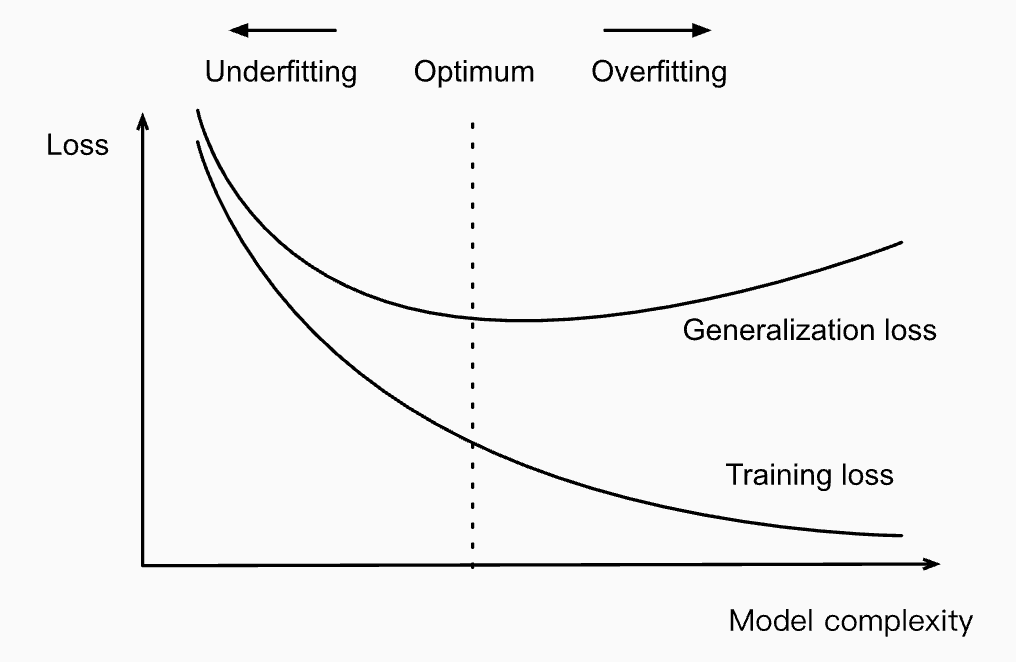
\includegraphics[width=0.7\columnwidth]{img/overfitting-vs-underfitting.png}
            \caption{Loss curve for overfitting and underfitting \footnotemark }
            \label{fig:overfitting_underfitting}
        \end{figure}
        \footnotetext{Source: \href{https://laptrinhx.com/boost-your-network-performance-1920317541/}{https://laptrinhx.com/boost-your-network-performance-1920317541/}}
    \end{answer}

    \item Bias-variance trade-off.
    \begin{InnerQandA}
        \item What’s the bias-variance trade-off?
        \begin{answer}
            In statistics and machine learning, the bias–variance tradeoff is the property of a model that the variance of the parameter estimated across samples can be reduced by increasing the bias in the estimated parameters. The bias–variance dilemma or bias–variance problem is the conflict in trying to simultaneously minimize these two sources of error that prevent supervised learning algorithms from generalizing beyond their training set (See Figure \ref{fig:bias-variance-complexity}).\\\\
            The bias–variance decomposition is a way of analyzing a learning algorithm's expected generalization error with respect to a particular problem as a sum of the bias and variance:
            \begin{align*}
                \text{MSE}\left(\hat{\theta}, \theta\right) = \text{Bias}^2\left(\hat{\theta}, \theta\right) + \text{Var}\left[ \hat{\theta} \right]
            \end{align*}
            where:
            \begin{align*}
                \text{MSE}\left(\hat{\theta}, \theta\right) &= \mathbb{E}_{D} \left[(\hat{\theta} - \theta)^2\right] \\
                \text{Bias}\left(\hat{\theta}, \theta \right) &= \mathbb{E}_{D}\left[\hat{\theta}\right] - \theta \\
                \text{Var}\left[\hat{\theta}\right] &= \mathbb{E}_{D} \left[ \left( \mathbb{E}_{D}\left[ \hat{\theta} \right] - \hat{\theta} \right)^2 \right]
            \end{align*}

            Let us show this equality with a quick proof:
            \begin{align*}
                \text{MSE}\left(\hat{\theta}, \theta \right) &= \mathbb{E}_{D} \left[ (\hat{\theta} - \theta)^2\right] \\
                &= \mathbb{E}_{D} \left[\left(\underbrace{\hat{\theta} - \mathbb{E}_{D}\left[ \hat{\theta} \right]}_{a} + \underbrace{\mathbb{E}_{D}\left[ \hat{\theta} \right] - \theta}_{b}\right)^2\right] \\
                &= \mathbb{E}_{D} \left[ \left( \hat{\theta} - \mathbb{E}_{d}\left[ \hat{\theta} \right] \right)^2 \right] + 2 \mathbb{E}_D \left[ \left( \hat{\theta} - \mathbb{E}_D \left[ \hat{\theta} \right] \right) \underbrace{\left( \mathbb{E}_D \left[ \hat{\theta} \right] - \theta \right)}_{\text{deterministic}} \right] + \mathbb{E}_D \left[ \left( \mathbb{E}_D \left[ \hat{\theta} \right] - \theta \right)^2 \right] \\
                &= \mathbb{E}_{D} \left[ \left( \hat{\theta} - \mathbb{E}_{d}\left[ \hat{\theta} \right] \right)^2 \right] + 2 \left( \mathbb{E}_D \left[ \hat{\theta} \right] - \theta \right) \mathbb{E}_D \left[ \left( \hat{\theta} - \mathbb{E}_D \left[ \hat{\theta} \right] \right)  \right] + \mathbb{E}_D \left[ \left( \mathbb{E}_D \left[ \hat{\theta} \right] - \theta \right)^2 \right] \\
                &= \mathbb{E}_{D} \left[ \left( \hat{\theta} - \mathbb{E}_{d}\left[ \hat{\theta} \right] \right)^2 \right] + 2 \left( \mathbb{E}_D \left[ \hat{\theta} \right] - \theta \right)  \underbrace{\left( \mathbb{E}_D \left[\hat{\theta}\right] - \mathbb{E}_D \left[ \hat{\theta} \right] \right)}_{0} + \mathbb{E}_D \left[ \left( \mathbb{E}_D \left[ \hat{\theta} \right] - \theta \right)^2 \right] \\
                &= \mathbb{E}_{D} \left[ \left( \hat{\theta} - \mathbb{E}_{d}\left[ \hat{\theta} \right] \right)^2 \right] + \mathbb{E}_D \left[ \underbrace{ \left( \mathbb{E}_D \left[ \hat{\theta} \right] - \theta \right)^2}_{\text{deterministic}} \right] \\
                &= \mathbb{E}_{D} \left[ \left( \hat{\theta} - \mathbb{E}_{d}\left[ \hat{\theta} \right] \right)^2 \right] + \left( \mathbb{E}_D \left[ \hat{\theta} \right] - \theta \right)^2 \\
                &= \text{Var}\left[\hat{\theta}\right] + \text{Bias}^2 \left(\hat{\theta}, \theta \right)
            \end{align*}

            (Source: \href{https://en.wikipedia.org/wiki/Bias\%E2\%80\%93variance\_tradeoff}{Wikipedia})

            \begin{figure}[htb!]
                \centering
                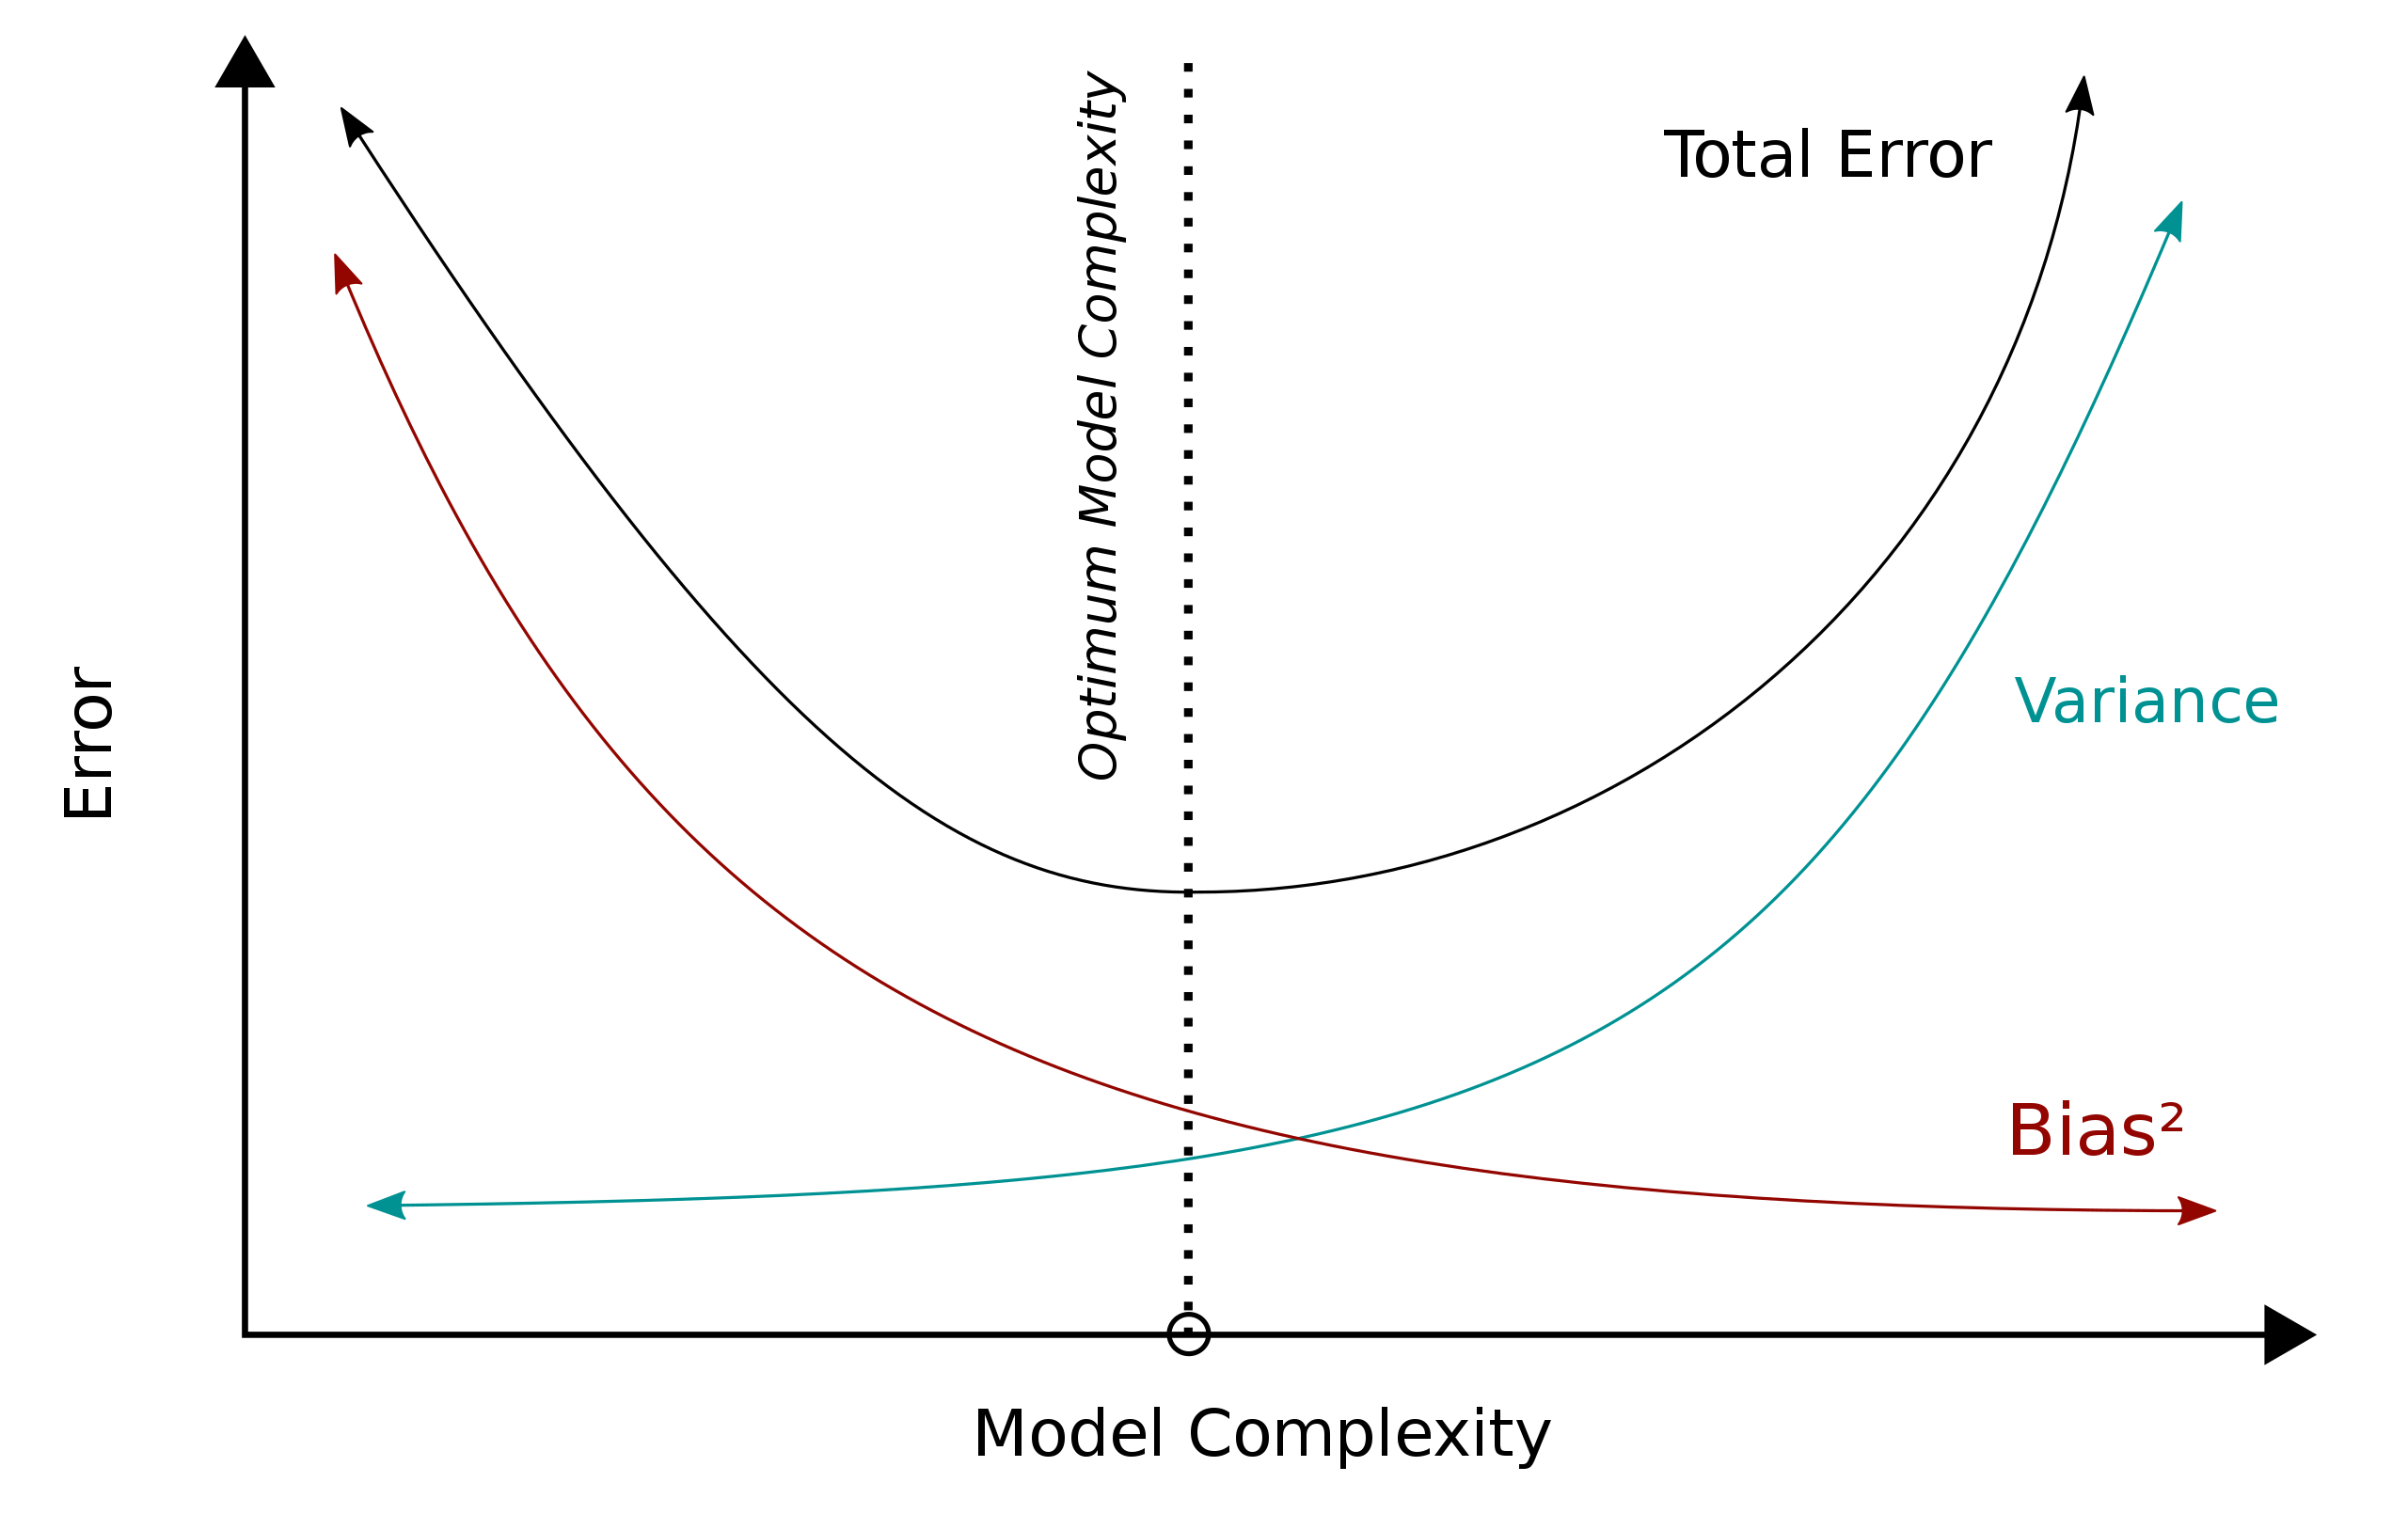
\includegraphics[width=0.6\columnwidth]{img/bias-var-complexity.png}
                \caption{Bias-Variance tradeoff\footnotemark.}
                \label{fig:bias-variance-complexity}
            \end{figure}
            \footnotetext{Source: \href{https://en.wikipedia.org/wiki/Bias\%E2\%80\%93variance\_tradeoff}{https://en.wikipedia.org/wiki/Bias\%E2\%80\%93variance\_tradeoff}}
            
        \end{answer}

        \item How’s this tradeoff related to overfitting and underfitting?
        \begin{answer}
            The relationship to overfitting and underfitting is as follows:
            \begin{itemize}
                \item The bias error is an error from erroneous assumptions in the learning algorithm. High bias can cause an algorithm to miss the relevant relations between features and target outputs (underfitting).
                \item The variance is an error from sensitivity to small fluctuations in the training set. High variance may result from an algorithm modeling the random noise in the training data (overfitting).
            \end{itemize}
            See also Figure \ref{fig:bias-variance-overfitting-underfitting}.

            \begin{figure}[htb!]
                \centering
                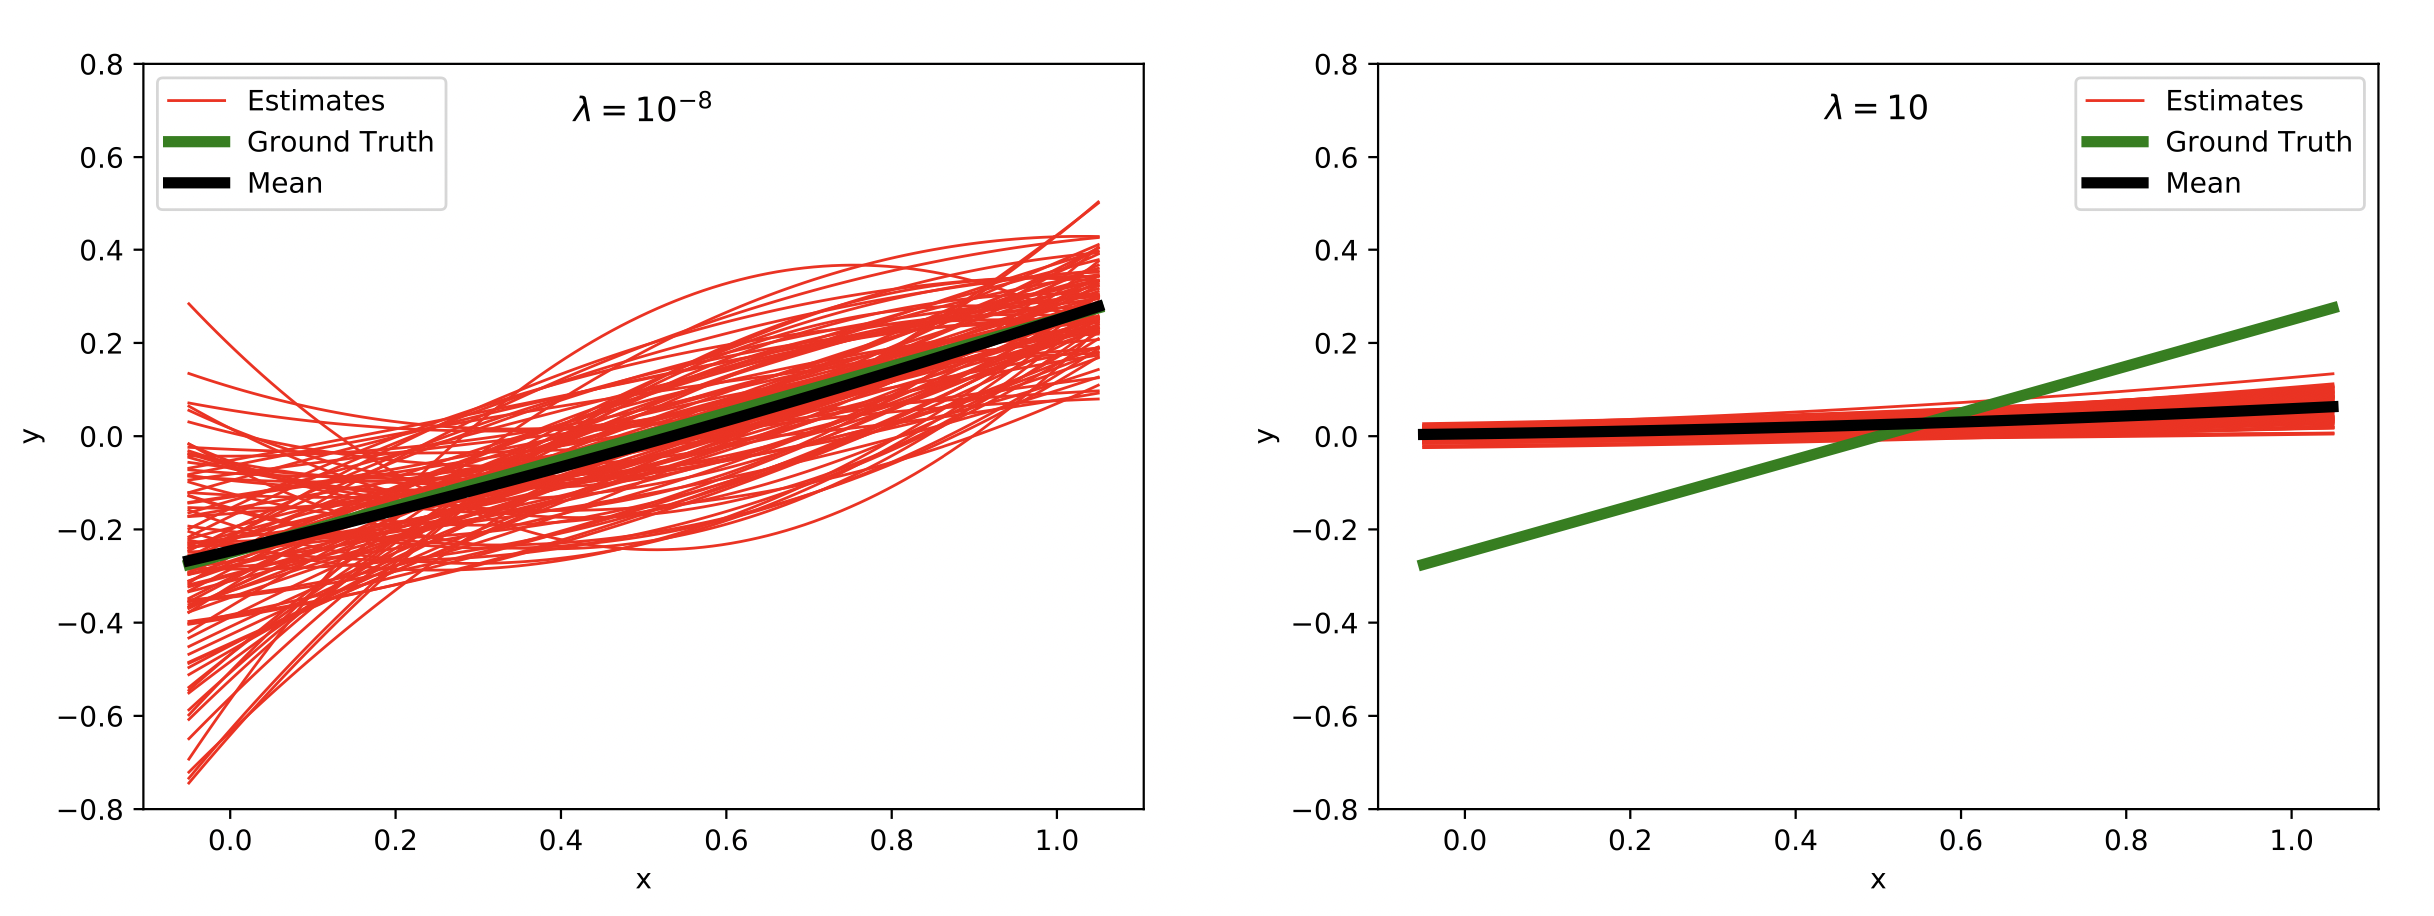
\includegraphics[width=0.9\columnwidth]{img/bias-var-overfit-underfit.png}
                \caption{The relationship of bias and variance to overfitting and underfitting. Left: High variance (overfitting); Right: High bias (underfitting).}
                \label{fig:bias-variance-overfitting-underfitting}
            \end{figure}

            (Source: \href{https://en.wikipedia.org/wiki/Bias%E2%80%93variance_tradeoff}{Wikipedia})
        \end{answer}

        \item How do you know that your model is high variance, low bias? What would you do in this case?
        \begin{answer}
            In high variance, low bias mode the model performs well on the training set but not on the test set. In this case one can: consider getting more training examples, try smaller set of features, reduce number of model parameters, increase regularization parameter $\lambda$.
        \end{answer}

        \item How do you know that your model is low variance, high bias? What would you do in this case?
        \begin{answer}
            In low variance, high bias mode, the model fails to even learn the data from the training set. In this case one can: add more features, increase number of model parameters, decrease regularization parameter $\lambda$.
        \end{answer}
    \end{InnerQandA}

    \item Cross-validation.
    \begin{InnerQandA}
        \item Explain different methods for cross-validation.
        \begin{answer}
            Cross-validation is a model validation technique for assessing how the results of a statistical analysis will generalize to an independent data set. Cross-validation is a resampling method that uses different portions of the data to test and train a model on different iterations. It is mainly used in settings where the goal is prediction, and one wants to estimate how accurately a predictive model will perform in practice. In a prediction problem, a model is usually given a dataset of known data on which training is run (training dataset), and a dataset of unknown data (or first seen data) against which the model is tested. The goal of cross-validation is to test the model's ability to generalize to an independent dataset (i.e., an unknown dataset, for instance from a real problem).\\\\
            There are several types of cross-validation:
            \begin{itemize}
                \item \textit{Holdout Method.} Remove a portion of the train data (eg. 20\%) and evaluate the trained model on this hold out set. Pro: the model only needs to be trained once. Con: a large portion of the train data is removed, might result in higher variance.

                \item \textit{K-Fold Cross-Validation.} Divide the train data in K folds (e.g 5 folds) and in Round-robin fashion, train on K-1 folds, while evaluating on the remaining fold. Pro: better use of the training data. Con: computationally expensive. 

                \item \textit{Stratified K-Fold Cross-Validation.} Makes sure that each fold contains approximately the same strata of samples of each class as the complete data set.

                \item \textit{Leave-P-Out Cross-Validation. } Leave P data points of the train data (eg. 5 data points) for evaluation, while training on the remaining N-P data points. Pro: lower variance. Con: computationally infeasible for large datasets.
            \end{itemize}

            (Source: \href{https://en.wikipedia.org/wiki/Cross-validation_(statistics)}{Wikipedia}, \href{https://www.upgrad.com/blog/cross-validation-in-machine-learning/}{Upgrad})
        \end{answer}

        \item Why don’t we see more cross-validation in deep learning?
        \begin{answer}
            With large datasets, it's very computationally expensive to perform K-fold / Leave-P-Out cross validation. These types of cross validation are most useful when the dataset is on the order of hundreds of examples. Therefore, in practice people usually perform the holdout method by splitting the dataset into train/val/test. 

            (Source: Yours truly, \href{https://www.quora.com/Is-cross-validation-heavily-used-in-deep-learning-or-is-it-too-expensive-to-be-used}{Yoshua Bengio})
        \end{answer}
    \end{InnerQandA}

    \item Train, valid, test splits.
    \begin{InnerQandA}
        \item What’s wrong with training and testing a model on the same data?
        \begin{answer}
            By training and testing on the same data, we get an overoptimistic estimate of the model's performance. Given enough model capacity, we can almost always overfit perfectly to the train set, but the model would perform poorly once deployed in production. 
        \end{answer}

        \item Why do we need a validation set on top of a train set and a test set?
        \begin{answer}
            Setting hyperparameters is very problem specific -- for each new dataset and each new method, it is very likely that we would need different values of the same hyperparameter. For this reason, we need to find the best hyperparameters before estimating the final model performance.\\\\
            However, if we merely have a train/test split, and evaluate the effectiveness of the chosen hyperparameter on the test set directly, we will get an overoptimistic estimate of the model's performance, since we are overfitting to the particular test set. Therefore, we typically split the dataset in train/val/test set, such that we fit our hyperparameters on the validation set, whereas we evaluate the final model performance once on the test set in order to get a realistic estimate of how the model will behave in production. 
        \end{answer}

        \item Your model’s loss curves on the train, valid, and test sets look like this (see Figure \ref{fig:train-val-test-curves}). What might have been the cause of this? What would you do?
        \begin{figure}[htb!]
            \centering
            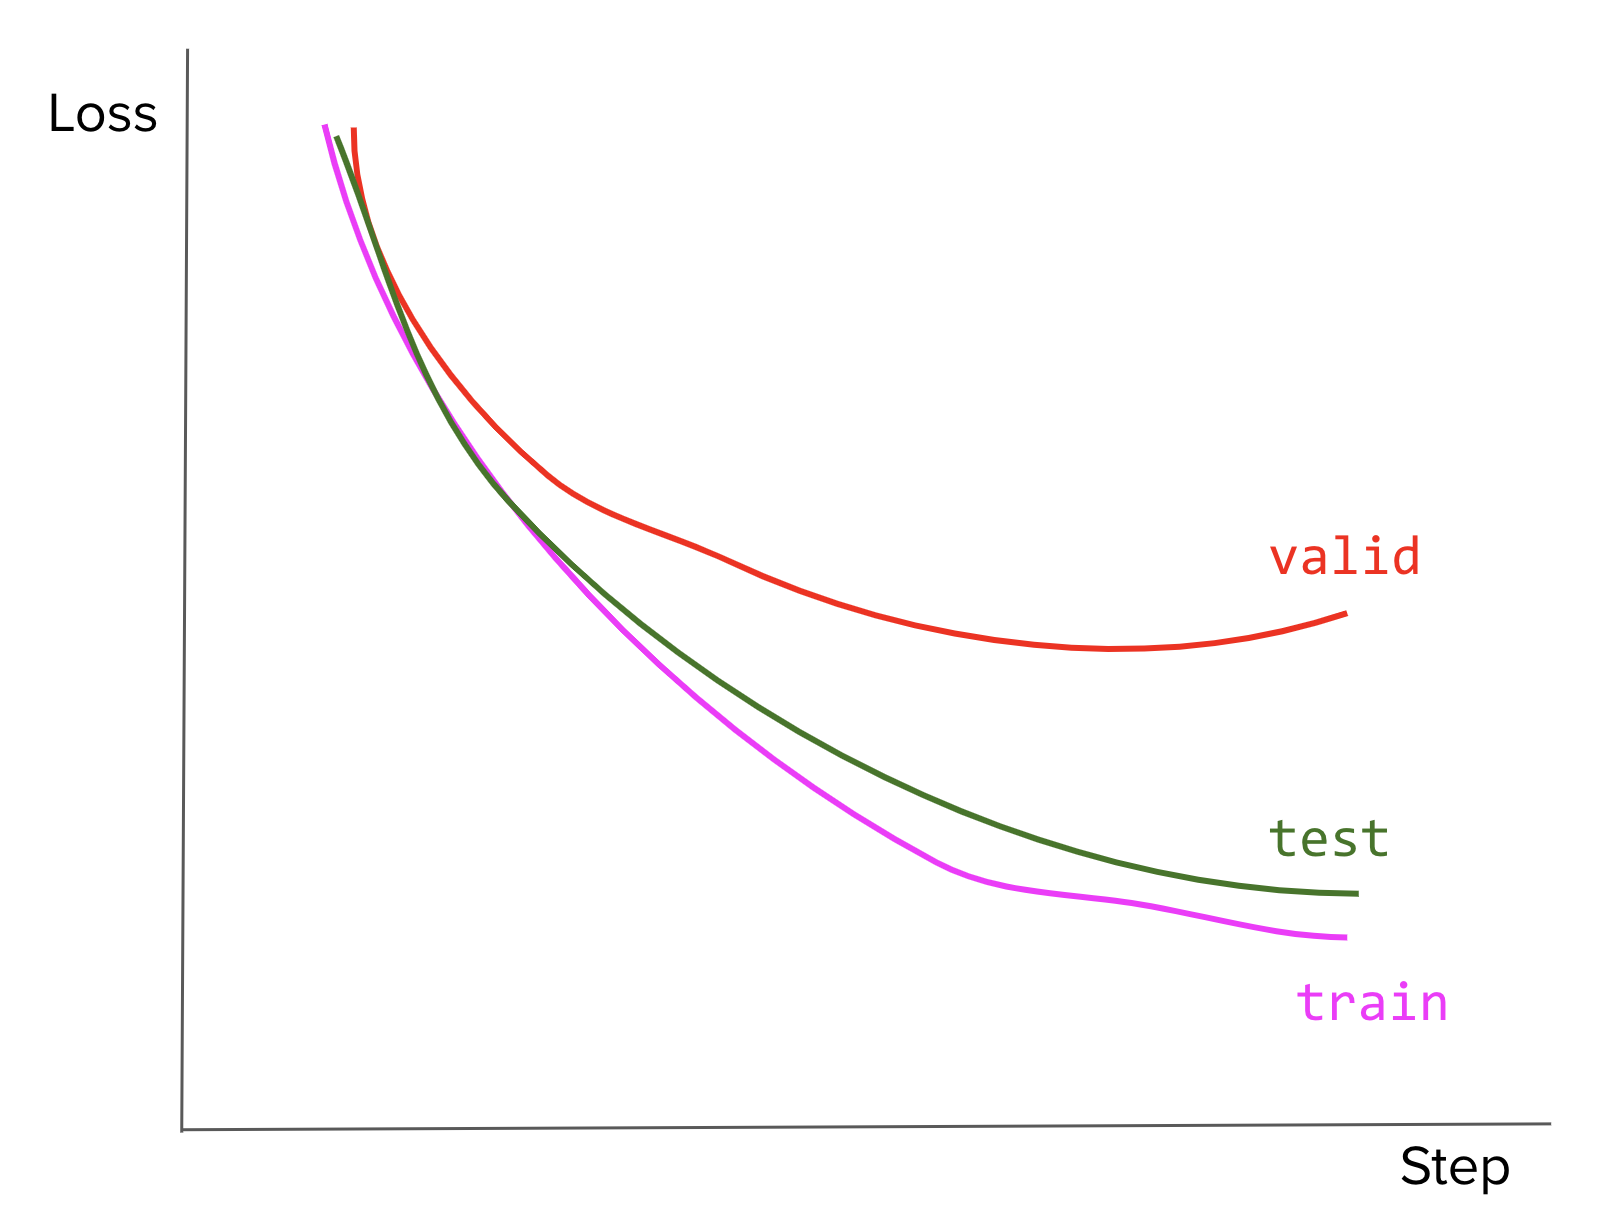
\includegraphics[width=0.5\columnwidth]{img/train-val-test-curves.png}
            \caption{Example of train, val, test curves.}
            \label{fig:train-val-test-curves}
        \end{figure}
        \begin{answer}
            It might be the case that the train set provides good enough coverage for the test distribution, but not for the entirety of the validation distribution. The cause might have been a bug in our splitting procedure, or we might simply have been unlucky with the random draws. A quick fix would be to check the implementation again, and perform a new split with a different random seed. 
        \end{answer}
    \end{InnerQandA}

    \item Your team is building a system to aid doctors in predicting whether a patient has cancer or not from their X-ray scan. Your colleague announces that the problem is solved now that they’ve built a system that can predict with 99.99\% accuracy. How would you respond to that claim?
    \begin{answer}
        Consider we have a dataset of 100,000 patients, where only 10 of them have been labeled as having cancer. \\\\
        A naive model always predicting that a given patient doesn't have cancer would have $\frac{99990}{100000} = 99.99\%$ accuracy, but is a totally useless model.
    \end{answer}

    \item F1 score.
    \begin{InnerQandA}
        \item What’s the benefit of F1 over the accuracy?
        \begin{answer}
            \begin{itemize}
                \item \textit{F1 score.} Pro: takes into account how the data is distributed. Useful when you have data with imbalance classes. Con: Less interpretable, since it is merely a trade-off between precision and recall.
                \item \textit{Accuracy.} Pro: easy to understand. Con: It does not take into account how the data is distributed.
            \end{itemize}

            (Source: \href{https://datascience.stackexchange.com/questions/65341/f1-score-vs-accuracy-which-metric-is-more-important}{StackExchange})
        \end{answer}

        \item Can we still use F1 for a problem with more than two classes. How?
        \begin{answer}
            For a multi-class classification problem, we don’t calculate an overall F1 score. Instead, we calculate the F1 score per class in a one-vs-rest manner. 

            (See more \href{https://www.baeldung.com/cs/multi-class-f1-score}{here}.)
        \end{answer}
    \end{InnerQandA}

    \item Given a binary classifier that outputs the following confusion matrix (Table \ref{tab:confusion-matrix}).

    \begin{table}[htb!]
    \centering
\begin{tabular}{|c|c|c|}
\hline
                      & \textbf{Predicted True} & \textbf{Predicted False} \\ \hline
\textbf{Actual True}  & 30                      & 20                       \\ \hline
\textbf{Actual False} & 5                       & 40                       \\ \hline
\end{tabular}
\caption{Confusion matrix}
\label{tab:confusion-matrix}
\end{table}
    
    \begin{InnerQandA}
        \item Calculate the model’s precision, recall, and F1.
        \begin{answer}
            \begin{align*}
                \text{Precision} &= \frac{\text{TP}}{\text{TP} + \text{FP}} = \frac{30}{30 + 5} = 0.85\\
                \text{Recall} &= \frac{\text{TP}}{\text{TP} + \text{FN}} = \frac{30}{30 + 20} = 0.6\\
                \text{F}_1 &= \frac{2 \cdot \text{Precision} \cdot \text{Recall}}{\text{Precision} + \text{Recall}} = \frac{2 \cdot 0.85 \cdot 0.6}{0.85 + 0.6} = 0.7034
            \end{align*}
        \end{answer}

        \item What can we do to improve the model’s performance?
        \begin{answer}
            The model is very conservative, in the sense that it rarely outputs the positive class (large number of False Negatives). The goal of improving the model's performance might be achieved by being more aggressive, and predicting the positive class more often. One way to do this is by lowering the threshold for which we predict a positive vs. negative class.
        \end{answer}
    \end{InnerQandA}

    \item Consider a classification where 99\% of data belongs to class A and 1\% of data belongs to class B.
    \begin{InnerQandA}
         \item If your model predicts A 100\% of the time, what would the F1 score be? (Hint: The F1 score when A is mapped to 0 and B to 1 is different from the F1 score when A is mapped to 1 and B to 0.)
         \begin{answer}
             First, let us suppose that A is mapped as the positive class, and B as the negative. Then, we would have the following confusion matrix:
            \begin{table}[htb!]
            \centering
            \begin{tabular}{|c|c|c|}
            \hline
                                  & \textbf{Predicted Pos} & \textbf{Predicted Neg} \\ \hline
            \textbf{Actual Pos}  & $0.99n$                      & 0                       \\ \hline
            \textbf{Actual Neg} & $0.01n$                       & 0                       \\ \hline
            \end{tabular}
            \end{table}

            From there, we obtain:
            \begin{align*}
                \text{Precision} &= \frac{0.99n}{0.99n + 0.01n} = 0.99\\
                \text{Recall} &= \frac{0.99n}{0.99n} = 1\\
                \text{F}_1 &=  \frac{2 \cdot 0.99 \cdot 1}{0.99 + 1} = 0.9949
            \end{align*}

            Now, let us suppose that A is mapped to the negative class, and B as to positive. Then, we would have the following confusion matrix:
            \begin{table}[htb!]
            \centering
            \begin{tabular}{|c|c|c|}
            \hline
                                  & \textbf{Predicted Pos} & \textbf{Predicted Neg} \\ \hline
            \textbf{Actual Pos}  & 0                      & $0.01$                       \\ \hline
            \textbf{Actual Neg} & 0                       & $0.99n$                       \\ \hline
            \end{tabular}
            \end{table}

            Then, we have:
            \begin{align*}
                \text{Precision} &= 0 \\
                \text{Recall} &= 0
            \end{align*}
            This implies that $\text{F}_1$ is undefined.
             
         \end{answer}

         \item If we have a model that predicts A and B at a random (uniformly), what would the expected F1 be?
         \begin{answer}
             Given that we choose each class with uniform probability, we obtain the following confusion matrix:

            \begin{table}[h!]
            \centering
            \begin{tabular}{|c|c|c|}
            \hline
                                  & \textbf{Predicted Pos} & \textbf{Predicted Neg} \\ \hline
            \textbf{Actual Pos}  & $0.5 \cdot 0.99n$                      & $0.5 \cdot 0.99n$                       \\ \hline
            \textbf{Actual Neg} & $0.5 \cdot 0.01n$                       & $0.5 \cdot 0.01n$                       \\ \hline
            \end{tabular}
            \end{table}
             From there, we can easily compute the expected F1 score:
             \begin{align*}
                 \text{Precision} &= \frac{0.5 \cdot 0.99n}{0.5 \cdot 0.99n + 0.5 \cdot 0.01n} = 0.99\\
                \text{Recall} &= \frac{0.5 \cdot 0.99n}{0.5 \cdot 0.99n + 0.5 \cdot 0.99n} = 0.5\\
                \text{F}_1 &=  \frac{2 \cdot 0.99 \cdot 0.5}{0.99 + 0.5} = 0.6644
             \end{align*}
         \end{answer}
    \end{InnerQandA}

    \item For logistic regression, why is log loss recommended over MSE (mean squared error)?
    \begin{answer}
        Log-loss is recommended over MSE because the optimization problem is convex in the former case, whereas in the latter it is non-convex. By operating on a convex loss-curve, we are guaranteed to arrive at the global minimum. \\\\
        For a function $f(x)$ to be convex, it is sufficient to show that $\frac{\partial^2 f}{\partial^2 x} \ge 0$ for all $x$. If the sign of the second derivative changes for different values of $x$, then $f(x)$ is not convex.\\\\
        Let us see why using MSE in logistic regression leads to a non-convex optimization problem. We have the following computation graph:
        \begin{align*}
            L(y, \hat{y}) = (y - \hat{y})^2 \quad\quad \hat{y} = \frac{1}{1 + \exp(-z)} \quad\quad z = \theta x
        \end{align*}
        Now, let us obtain the second derivative:
        \begin{align*}
            \frac{\partial L}{\partial \theta} &= \frac{\partial L}{\partial \hat{y}} \cdot \frac{\partial \hat{y}}{\partial z} \cdot \frac{\partial z}{\partial \theta} \\
            &= -2(y - \hat{y}) \cdot (\hat{y}(1 - \hat{y})) \cdot x \\
            &= -2x \left[ (y - \hat{y})(\hat{y} - \hat{y}^2) \right] \\
            &= -2x \left[ y\hat{y} - y\hat{y}^2 - \hat{y}^2 + \hat{y}^3 \right] \\\\
            \frac{\partial L}{\partial^2 \theta} &= -2x \left[ y\hat{y}(1-\hat{y})x - 2 y \hat{y} \hat{y} (1-\hat{y})x - 2 \hat{y}\hat{y}(1-\hat{y})x + 3\hat{y}^2\hat{y}(1-\hat{y})x \right] \\
            &= -2x^2\hat{y}(1-\hat{y}) \left[ y - 2y\hat{y} - 2\hat{y}^2 +3\hat{y}^2 \right]
        \end{align*}
        Since $2 \ge 0$, $x^2 \ge 0$ and $\hat{y}(1-\hat{y}) \ge 0$, we can exclude them from our analysis of the sign of the second derivative.\\\\
        Now, consider the case when $y=0$. Then:
        \begin{align*}
            \frac{\partial^2 L}{\partial^2 \theta} &\propto -\left[ -2\hat{y}^2 + 3\hat{y}^2 \right] \\
            &= -\left[ 3\hat{y} (\hat{y} - \frac{2}{3})\right]
        \end{align*}
        Now, notice when $\hat{y} \in \left[ 0, \frac{2}{3}\right]$ then $\frac{\partial^2 L}{\partial^2 \theta} \ge 0$, but when $\hat{y} \in \left[ \frac{2}{3}, 1\right]$ then $\frac{\partial^2 L}{\partial^2 \theta} \le 0$. Therefore, we proved that the MSE loss is not convex wrt $\theta$.\\\\
        Now, let us see why using the Log-loss in logistic regression leads to a convex optimization problem. We have the following computation graph:
        \begin{align*}
            L(y, \hat{y}) = - \left[y\log(\hat{y}) + (1-y) \log(1-\hat{y})\right] \quad\quad \hat{y} = \frac{1}{1 + \exp(-z)} \quad\quad z = \theta x
        \end{align*}
        Now, let us obtain the second derivative:
        \begin{align*}
            \frac{\partial L}{\partial \theta} &= \frac{\partial L}{\partial \hat{y}} \cdot \frac{\partial \hat{y}}{\partial z} \cdot \frac{\partial z}{\partial \theta} \\
            &= -\left[ \frac{y}{\hat{y}} - \frac{1-y}{1-\hat{y}} \right]\hat{y}(1-\hat{y})x \\
            &= x \left[ \frac{\hat{y}(1-\hat{y})(1-y)}{(1-\hat{y})} - \frac{\hat{y}(1-\hat{y})y}{\hat{y}} \right] \\
            &= x \left[ \hat{y}(1-y) - y(1-\hat{y}) \right] \\\\
            \frac{\partial^2 L}{\partial^2 \theta} &= x \left[ \hat{y}(1-\hat{y})x(1-y) + y\hat{y}(1-\hat{y})x \right] \\
            &= x^2 \hat{y} (1-\hat{y}) \left[ (1 - y) + y \right] \\
            &= x^2\hat{y}(1-\hat{y})\\
            &\ge 0
        \end{align*}
        Therefore, we obtain that the Log-loss is convex wrt. $\theta$.

        (Source: \href{https://towardsdatascience.com/why-not-mse-as-a-loss-function-for-logistic-regression-589816b5e03c}{TowardsDataScience})
    \end{answer}

    \item When should we use RMSE (Root Mean Squared Error) over MAE (Mean Absolute Error) and vice versa?
    \begin{answer}
        In general, (R)MSE is more sensitive to outliers than MAE, and the model will be more skewed towards them. Using one loss over the other typically comes down to how important is it to perform well on outliers.\\\\
         In many circumstances it makes sense to give more weight to points further away from the mean. For example, being off by 10 is more than twice as bad as being off by 5. In such cases RMSE is a more appropriate measure of error. \\\\
         If being off by 10 is just twice as bad as being off by 5, then MAE is more appropriate.

         (Source: \href{https://stats.stackexchange.com/questions/48267/mean-absolute-error-or-root-mean-squared-error}{StackExchange})
    \end{answer}

    \item Show that the negative log-likelihood and cross-entropy are the same for binary classification tasks.
    \begin{answer}
        I am not sure I understand the question 100\%, so I will give an answer to the following instead (perhaps the author meant this): Show that the Binary Cross Entropy loss can be naturally derived from the maximum likelihood principle under the assumption that the likelihood of the output is a Bernoulli random variable:
        \begin{align*}
            p(y \g x, w) = \hat{y}^y (1-\hat{y})^{1-y} \quad\quad \hat{y} = f_w(x)
        \end{align*}
        During training we wish to maximize the likelihood:
        \begin{align*}
            w^* &= \argmax_{w} p(Y \g X, w) \\
            &= \argmax_{w} \prod_{i=1}^n p(y_i \g x_i, w) &\text{(iid assumption)} \\
            &= \argmax_{w} \sum_{i=1}^n \log p(y_i \g x_i, w) \\
            &= \argmax_{w} \sum_{i=1}^n y_i\log(\hat{y}_i) + (1-y_i)\log(1-\hat{y_i}) \\
            &= \argmin_{w} \underbrace{\sum_{i=1}^n - \left[ y_i\log(\hat{y}_i) + (1-y_i)\log(1-\hat{y}_i)\right]}_{\text{Binary Cross Entropy}}
        \end{align*}
        Which in fact, ends up minimizing the Binary Cross Entropy loss. \\\\
        Perhaps my confusion stems from misunderstanding what exactly people mean when they say ``log-loss'' or ``negative log-likelihood'' for a particular loss: every loss commonly used today is derived from the maximum likelihood principle when we assume a certain form for the likelihood: Bernoulli likelihood $\rightarrow$ Binary Cross-Entropy; Categorical likelihood $\rightarrow$ Categorical Cross Entropy; Gaussian likelihood $\rightarrow$ MSE; Laplace likelihood $\rightarrow$ MAE. There is no one particular loss that is a ``log-loss'', many of them are!!!\\
        (/* end rant */)
    \end{answer}

    \item For classification tasks with more than two labels (e.g. MNIST with 10 labels), why is cross-entropy a better loss function than MSE?
    \begin{answer}
        Similarly as before, let us see how we can derive the Cross Entropy loss from the maximum likelihood principle. Assume that the likelihood of the output is a Categorical random variable:
        \begin{align*}
            p(y \g x, w) = \prod_{c=1}^C \hat{y}_c^{y_c} \quad\quad \hat{y} = f_w(x)
        \end{align*}
        where $y \in \R^C$ is a one-hot encoding for the true class. During training we wish to maximize the likelihood:
        \begin{align*}
            w^* &= \argmax_{w} p(Y \g X, w) \\
            &= \argmax_{w} \prod_{i=1}^n p(y_i \g x_i, w) &\text{(iid assumption)} \\
            &= \argmax_{w} \sum_{i=1}^n \log p(y_i \g x_i, w) \\
            &= \argmax_{w} \sum_{i=1}^n \sum_{c=1}^C y_{i, c} \log (\hat{y}_{i, c}) \\
            &= \argmin_{w} \underbrace{\sum_{i=1}^n \sum_{c=1}^C - y_{i, c} \log (\hat{y}_{i, c})}_{\text{Cross Entropy}}
        \end{align*}
        Which results in minimizing the Cross Entropy loss. \\\\
        In contrast, now assume that the likelihood of the output is a Normal random variable:
        \begin{align*}
            p(y \g x, w) = \frac{1}{\sqrt{2\pi \sigma^2}} \exp \left ( -\frac{(y - \hat{y})^2}{2\sigma^2} \right) \quad \quad \hat{y} = f_w(x)
        \end{align*}
        
        \begin{align*}
            w^* &= \argmax_{w} p(Y \g X, w) \\
            &= \argmax_{w} \prod_{i=1}^n p(y_i \g x_i, w) &\text{(iid assumption)} \\
            &= \argmax_{w} \sum_{i=1}^n \log p(y_i \g x_i, w) \\
            &= \argmax_{w} \sum_{i=1}^n \left [\log \left( \frac{1}{\sqrt{2\pi \sigma^2}} \right) -  \frac{(y_i - \hat{y}_i)^2}{2\sigma^2} \right]\\
            &= \argmax_{w} \sum_{i=1}^n -\frac{(y_i - \hat{y}_i)^2}{2\sigma^2} \\
            &= \argmin_{w} \underbrace{\sum_{i=1}^n (y_i - \hat{y}_i)^2}_{\text{Mean Squared Error}}
        \end{align*} 
        Which results in minimizing the Mean Squared Error loss. \\\\
        When doing a multi-class classification problem, the assumption about the likelihood being a Categorical random variable as opposed to a Normal random variable is more natural, hence the common use of the Cross Entropy loss function. \\\\
        In fact, the same line of reasoning can be applied for answering Question 10 of this section. 
    \end{answer}

    \item Consider a language with an alphabet of 27 characters. What would be the maximal entropy of this language?
    \begin{answer}
        The entropy is maximized when we have the least amount of knowledge about predicting the next character in a sequence, given the previous characters. This corresponds to a uniform distribution, which would imply that the probability of every character is $\frac{1}{27}$.
    \end{answer}

    \item A lot of machine learning models aim to approximate probability distributions. Let’s say P is the distribution of the data and Q is the distribution learned by our model. How do measure how close Q is to P?
    \begin{answer}
        In mathematical statistics, the Kullback–Leibler divergence, denoted $\KL{P}{Q}$, is a type of statistical distance: a measure of how one probability distribution $P$ is different from a second, reference probability distribution $Q$:
        \begin{align*}
            \KL{P}{Q} = \sum_{x \in \mathcal{X}} P(x) \log \left( \frac{P(x)}{Q(x)} \right)
        \end{align*}
        A simple interpretation of the KL divergence of $P$ from $Q$ is the expected excess surprise from using $Q$ as a model when the actual distribution is $P$. \\\\
        While it is a distance, it is not a metric, the most familiar type of distance: it is not symmetric in the two distributions, and does not satisfy the triangle inequality:
        \begin{align*}
            d(p, q) \le d(p, r) + d(r, q)
        \end{align*}
        We will give a counter-example to prove that the triangle inequality is not satisfied. Let:
        \begin{align*}
            \mathcal{X} &= \{0, 1\} \\
            P(x) &= \begin{cases}
                \frac{1}{2} & \text{if } x = 0 \\
                \frac{1}{2} & \text{if } x = 1
            \end{cases} \\
            R(x) &= \begin{cases}
                \frac{1}{4} & \text{if } x = 0 \\
                \frac{3}{4} & \text{if } x = 1
            \end{cases} \\
            Q(x) &= \begin{cases}
                \frac{1}{10} & \text{if } x = 0 \\
                \frac{9}{10} & \text{if } x = 1
            \end{cases}        
        \end{align*}
        Then, the triangle inequality should state:
        \begin{align*}
            \KL{P}{Q} &\le \KL{P}{R} + \KL{R}{Q} \\
            \sum_{x \in \mathcal{X}} P(x) \log \left( \frac{P(x)}{Q(x)} \right) &\le \sum_{x \in \mathcal{X}} P(x) \log \left( \frac{P(x)}{R(x)} \right) + \sum_{x \in \mathcal{X}} R(x) \log \left( \frac{R(x)}{Q(x)} \right) \\
            0.51 &\le 0.14 + 0.09 \\
            0.51 &\le 0.24
        \end{align*}
        which is clearly not true.

        (Source: \href{https://en.wikipedia.org/wiki/Kullback%E2%80%93Leibler_divergence}{Wikipedia}, \href{https://ai.stackexchange.com/questions/18019/why-does-the-kl-divergence-not-satisfy-the-triangle-inequality}{StackExchange})
    \end{answer}

    \item MPE (Most Probable Explanation) vs. MAP (Maximum A Posteriori)
    \begin{InnerQandA}
        \item How do MPE and MAP differ?
        \begin{answer}
            \begin{itemize}
                \item \textit{Most Probable Explanation}: Given observations for some variables, compute the most likely assignment for all remaining variables. 
                \item \textit{Maximum A Posteriori}: Given observations for some variables, compute the most likely assignment for a subset of the remaining variables. MPE is a special case of MAP.
            \end{itemize}
        \end{answer}

        \item Give an example of when they would produce different results.
        \begin{answer}
            Suppose we have three binary random variables $X$, $Y$, and $Z$ with a joint distribution as described in Table \ref{tab:joint-binary-vars}.
            \begin{table}[h!]
            \centering
            \begin{tabular}{|c|c|c|c|}
            \hline
            \textbf{X} & \textbf{Y} & \textbf{Z} & \textbf{P(X, Y, Z)} \\ \hline
            0          & 0          & 0          & 0.27000             \\ \hline
            0          & 0          & 1          & 0.00930             \\ \hline
            0          & 1          & 0          & 0.21500             \\ \hline
            0          & 1          & 1          & 0.10750             \\ \hline
            1          & 0          & 0          & 0.09690             \\ \hline
            1          & 0          & 1          & 0.19380             \\ \hline
            1          & 1          & 0          & 0.05375             \\ \hline
            1          & 1          & 1          & 0.05375             \\ \hline
            \end{tabular}
            \caption{Joint distribution for $X$, $Y$, $Z$}
            \label{tab:joint-binary-vars}
            \end{table}

            Now imagine we have observed $Y = 0$, and are interested in the most probable value for $X$. While we are not intersted in $Z$, it's a quantity that is a part of our distribution, hence we cannot ignore it completely. \\\\
            If we want to perform Maximum A Posteriori estimation, then we marginalize over $Z$:
            \begin{align*}
                &P(X = 0 \g Y = 0) \\
                = &\frac{P(X = 0, Y = 0)}{P(Y = 0)} \\
                = &\frac{P(X=0, Y=0, Z=0) + P(X = 0, Y = 0, Z = 1)}{P(X = 0, Y = 0, Z = 0) + P(X = 0, Y = 0, Z = 1) + P(X = 1, Y = 0, Z = 0) + P(X = 1, Y = 0, Z = 1)} \\
                = &\frac{0.2793}{0.57} \\
                = &0.49 \\\\
                \implies &P(X=1 \g Y=0) = 1 - P(X = 0 \g Y=0) = 0.51
            \end{align*}
            Therefore, according to the MAP principle, the most likely value for $X$ is $1$, given that $Y = 0$. \\\\
            Alternatively, if we go down the Maximum Probable Explanation route, we have to maximize over all pairs of conditional probabilities where $Y = 0$:
            \begin{align*}
                P(X = 0, Z = 0 \g Y = 0) &= \frac{P(X = 0, Y=0, Z=0)}{P(Y=0)} = \frac{0.27}{0.57} = 0.4736 \\
                P(X = 0, Z = 1 \g Y = 0) &= \frac{P(X = 0, Y=0, Z=1)}{P(Y=0)} = \frac{0.0093}{0.57} = 0.0163 \\
                P(X = 1, Z = 0 \g Y = 0) &= \frac{P(X = 1, Y=0, Z=0)}{P(Y=0)} = \frac{0.0969}{0.57} = 0.17 \\
                P(X = 1, Z = 1 \g Y = 0) &= \frac{P(X = 1, Y=0, Z=1)}{P(Y=0)} = \frac{0.1938}{0.57} = 0.34
            \end{align*}
            From the 4 pairs, we maximize the (joint) conditional when $X=0$ (and $Z=0$).  \\\\
            With this, we showed that MAP and MPE can give different solutions, given a same observation.

        
            (See more \href{https://www.quora.com/What-are-the-cases-in-which-Most-Probable-Explanation-MPE-tasks-do-not-generalize-to-Maximum-A-Posteriori-MAP-task}{here})
        \end{answer}
    \end{InnerQandA}

    \item Suppose you want to build a model to predict the price of a stock in the next 8 hours and that the predicted price should never be off more than 10\% from the actual price. Which metric would you use?
    \begin{answer}
        I am not sure if we can define a metric that predicted price is \textit{never} off by more than 10\%, but using Mean Absolute Percentage Error we can investigate whether our model \textit{on average} is not off by more than 10 \%. \\\\
        The Mean Absolute Percentage Error (MAPE) is a measure of prediction accuracy of a forecasting method in statistics. It usually expresses the accuracy as a ratio defined by the formula:
        \begin{align*}
            \text{MAPE} = \frac{100\%}{n} \sum_{i=1}^n \left \vert  \frac{A_t - F_t}{A_t} \right \vert
        \end{align*}
        where $A_t$ is the actual value and $F_t$ is the forecast value.

        (Source: \href{https://en.wikipedia.org/wiki/Mean_absolute_percentage_error}{Wikipedia})
    \end{answer}
\end{QandA}

\section{Machine Learning Algorithms}
\subsection{Classical machine learning}
\begin{QandA}
    \item What are the basic assumptions to be made for linear regression?
    \begin{answer}
        There are four assumptions associated with a linear regression model:
        \begin{itemize}
            \item \textit{Linearity}: The relationship between X and the mean of Y is linear.
            \item \textit{Homoscedasticity}: The variance of residual is the same for any value of X.
            \item \textit{Independence}: Observations are independent of each other.
            \item \textit{Normality}: For any fixed value of X, Y is normally distributed.
        \end{itemize}
        (See more \href{https://sphweb.bumc.bu.edu/otlt/MPH-Modules/BS/R/R5_Correlation-Regression/R5_Correlation-Regression4.html}{here})
    \end{answer}

    \item What happens if we don’t apply feature scaling to logistic regression?
    \begin{answer}
        Standardization isn't required for logistic regression. The main goal of standardizing features is to help convergence of the technique used for optimization.\\\\
        However, if one uses regularization (eg. Lasso or Ridge), then standardization is required since the obtained solutions are not equivariant under scaling the input.

        (Source: \href{https://stats.stackexchange.com/questions/48360/is-standardization-needed-before-fitting-logistic-regression}{StackExchange})
    \end{answer}

    \item What are the algorithms you’d use when developing the prototype of a fraud detection model?
    \begin{answer}
        Decision Trees, Random Forests, Gradient Boosting Machine, Support Vector Machine, K-Nearest Neighbors, \ldots
    \end{answer}

    \item Feature selection.
    \begin{InnerQandA}
        \item Why do we use feature selection?
        \begin{answer}
            Feature selection is the process of selecting a subset of relevant features for use in model construction. Feature selection techniques are used for several reasons:
            \begin{itemize}
                \item simplification of models to make them easier to interpret by users
                \item shorter training times
                \item to avoid the curse of dimensionality
            \end{itemize}
        The central premise when using a feature selection technique is that the data contains some features that are either redundant or irrelevant, and can thus be removed without incurring much loss of information. Redundant and irrelevant are two distinct notions, since one relevant feature may be redundant in the presence of another relevant feature with which it is strongly correlated.\\\\
        Feature selection techniques should be distinguished from feature extraction. Feature extraction creates new features from functions of the original features, whereas feature selection returns a subset of the features. Feature selection techniques are often used in domains where there are many features and comparatively few samples. Archetypal cases for the application of feature selection include the analysis of written texts and DNA microarray data, where there are many thousands of features, and a few tens to hundreds of samples.
        \end{answer}

        \item What are some of the algorithms for feature selection? Pros and cons of each.
        \begin{answer}
            There are three main categories of feature selection techniques:
            \begin{itemize}
                \item \textit{Wrapper methods} use a predictive model to score feature subsets. Each new subset is used to train a model, which is tested on a hold-out set. Counting the number of mistakes made on that hold-out set (the error rate of the model) gives the score for that subset. As wrapper methods train a new model for each subset, they are very computationally intensive, but usually provide the best performing feature set for that particular type of model or typical problem. Common approaches are greedy forward (start with the best performing variable against the target, and iteratively add new ones), and greedy backward (start with all features, and iteratively truncate one by one) selection.
                \item \textit{Filter methods} use a proxy measure instead of the error rate to score a feature subset. This measure is chosen to be fast to compute, while still capturing the usefulness of the feature set. Common measures include the mutual information, Pearson correlation coefficient, Relief-based algorithms, inter/intra class distance, and the scores of significance tests for each class/feature combinations. Filters are usually less computationally intensive than wrappers, but they produce a feature set which is not tuned to a specific type of predictive model. This lack of tuning means a feature set from a filter is more general than the set from a wrapper, usually giving lower prediction performance than a wrapper. However the feature set doesn't contain the assumptions of a prediction model, and so is more useful for exposing the relationships between the features. Many filters provide a feature ranking rather than an explicit best feature subset, and the cut off point in the ranking is chosen via cross-validation. 
                \item \textit{Embedded methods} perform feature selection as part of the model construction process. The exemplar of this approach is the LASSO method for constructing a linear model, which penalizes the regression coefficients with an L1 penalty, shrinking many of them to zero. Any features which have non-zero regression coefficients are 'selected' by the LASSO algorithm.
            \end{itemize}

            (Source: \href{https://en.wikipedia.org/wiki/Feature_selection}{Wikipedia})
        \end{answer}
    \end{InnerQandA}

    \item k-means clustering.
    \begin{InnerQandA}
        \item How would you choose the value of k?
        \begin{answer}
            While there is no universally optimal way to set the value of k, there are two approaches that have empirically worked well in practice:
            \begin{itemize}
                \item \textit{Elbow Curve Method.} The idea is to perform k-means clustering for several values of k, plot the sum of squared distances of samples to their closest cluster center, and pick the first value of k for which the aforementioned metric plateaus (see Figure \ref{fig:elbow}).
                \begin{figure}[htb!]
                    \centering
                    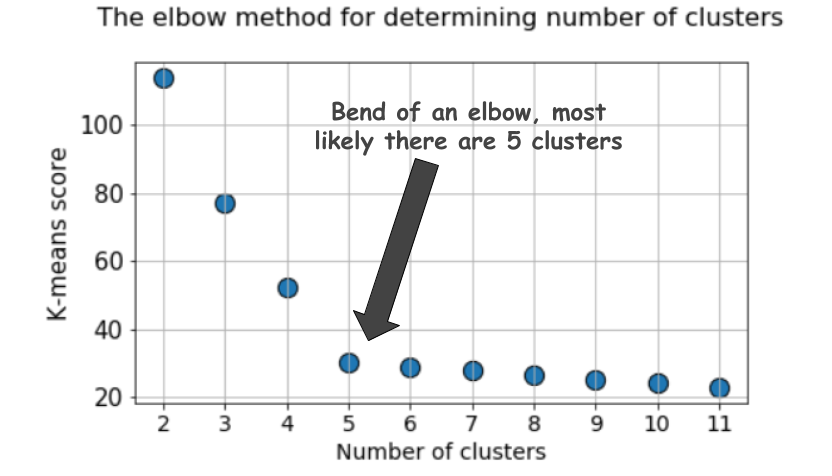
\includegraphics[width=0.9\columnwidth]{img/elbow.png}
                    \caption{Choosing the optimal k according to the Elbow method \footnotemark }
                    \label{fig:elbow}
                \end{figure}
                \footnotetext{Source: \href{https://towardsdatascience.com/clustering-metrics-better-than-the-elbow-method-6926e1f723a6}{https://towardsdatascience.com/clustering-metrics-better-than-the-elbow-method-6926e1f723a6}}

                \item \textit{Silhouette coefficient.} Similarly as before, the idea is to perform k-means clustering for several values of k, plot the mean Silhouette coefficient (see below), and pick the value of k for which the metric is maximized. \\\\
                The Silhouette coefficient is calculated as the (normalized) difference between the mean nearest-cluster distance ($b$) and the mean intra-cluster distance ($a$):
                \begin{align*}
                    \text{Silhouette score} = \frac{b-a}{\max\{b, a\}}
                \end{align*}
                We obtain the best value of $1$ when $a < b$:
                \begin{align*}
                    \text{Silhouette score} = \frac{b-a}{\max\{b, a\}} = \frac{b-a}{b} = 1 - \frac{a}{b}
                \end{align*}
                which occurs when we minimize the ratio $\frac{a}{b}$, by either minimizing the within cluster distances, or maximizing the distances to the nearest cluster. \\\\
                Similarly, we obtain the worst value of $-1$ when $a > b$:
                \begin{align*}
                    \text{Silhouette score} = \frac{b-a}{\max\{b, a\}} = \frac{b-a}{a} = \frac{b}{a}-1
                \end{align*}
                which occurs when we minimize the ratio $\frac{b}{a}$, by either minimizing the distances to the nearest cluster, or maximizing the distances within the cluster.

                (Source: \href{https://scikit-learn.org/stable/modules/generated/sklearn.metrics.silhouette_score.html}{SciKit})
            \end{itemize}
        \end{answer}

        \item If the labels are known, how would you evaluate the performance of your k-means clustering algorithm?
        \begin{answer}
            Given that labels are known, we can evaluate the performance of our clustering with:
            \begin{itemize}
                \item \textit{Purity.} Purity is a measure of the extent to which clusters contain a single class. Its calculation can be thought of as follows: For each cluster, count the number of data points from the most common class in said cluster. Now take the sum over all clusters and divide by the total number of data points. Formally, given some set of clusters $M$ and some set of classes $C$, both partitioning $N$ data points, the metric can be defined as follows:
                \begin{align*}
                    \text{Purity} = \frac{1}{N} \sum_{m \in M} \max_{c \in C} \vert m \cap c \vert
                \end{align*}
                This measure doesn't penalize having many clusters, and more clusters will make it easier to produce a high purity. A purity score of 1 is always possible by putting each data point in its own cluster. Also, purity doesn't work well for imbalanced data, where even poorly performing clustering algorithms will give a high purity value. For example, if a size 1000 dataset consists of two classes, one containing 999 points and the other containing 1 point, then every possible partition will have a purity of at least 99.9\%.
                \item \textit{Rand index}. The Rand index  computes the fraction of correct pairwise assignments between the clustering output and the ground truth. Formally:
                \begin{align*}
                    RI = \frac{TP + TN}{TP + FP + FN + TN}
                \end{align*}
                where $TP$ is the number of pairs of points that are clustered together in the predicted partition and in the ground truth partition, $FP$ is the number of pairs of points that are clustered together in the predicted partition but not in the ground truth partition etc. If the dataset is of size $N$, then $TP + FP + FN + TN = {N \choose 2}$.
            \end{itemize}
        \end{answer}

        \item How would you do it if the labels aren’t known?
        \begin{answer}
            If the labels are not known, as we have seen before, we can compute the Silhouette coefficient to get a better idea of the goodness of cluster assignment. Moreover, let us introduce 2 more techniques:
            \begin{itemize}
                \item \textit{Davies–Bouldin index.} The Davies–Bouldin index can be calculated by the following formula:
                \begin{align*}
                    DB = \frac{1}{M}\sum_{m \in M} \max_{k \neq m} \left( \frac{\sigma_m + \sigma_k}{d(c_m, c_k)} \right)
                \end{align*}
                where $M$ is the number of clusters, $c_m$ is the centroid of cluster $m$, $\sigma_m$ is the average distance of all elements in cluster $m$ to the centroid $c_m$, and $d(c_m, c_k)$ is the distance between the centroids $c_m$ and $c_k$. Since algorithms that produce clusters with low intra-cluster distances (high intra-cluster similarity) and high inter-cluster distances (low inter-cluster similarity) will have a low Davies–Bouldin index, the clustering algorithm that produces a collection of clusters with the smallest Davies–Bouldin index is considered the best algorithm based on this criterion. 

                \item \textit{Dunn index.} The Dunn index aims to identify dense and well-separated clusters. It is defined as the ratio between the minimal inter-cluster distance to maximal intra-cluster distance. For each cluster partition, the Dunn index can be calculated by the following formula:
                \begin{align*}
                    D = \frac{\max_{1 \le m < k \le M}d(m, k)}{\max_{1 \le t \le M} d'(t)}
                \end{align*}
                where $d(m, k)$ represents the distance between clusters $m$ and $k$, and $d'(t)$ measures the intra-cluster distance of cluster $t$. The inter-cluster distance $d(m,k)$ between two clusters may be any number of distance measures, such as the distance between the centroids of the clusters. Similarly, the intra-cluster distance $d'(t)$ may be measured in a variety ways, such as the maximal distance between any pair of elements in cluster $t$. Since internal criterion seek clusters with high intra-cluster similarity and low inter-cluster similarity, algorithms that produce clusters with high Dunn index are more desirable.
            \end{itemize}
        \end{answer}

        \item Given the following dataset (see Figure \ref{fig:k-means-example}), can you predict how K-means clustering works on it? Explain.
        \begin{figure}[h!]
            \centering
            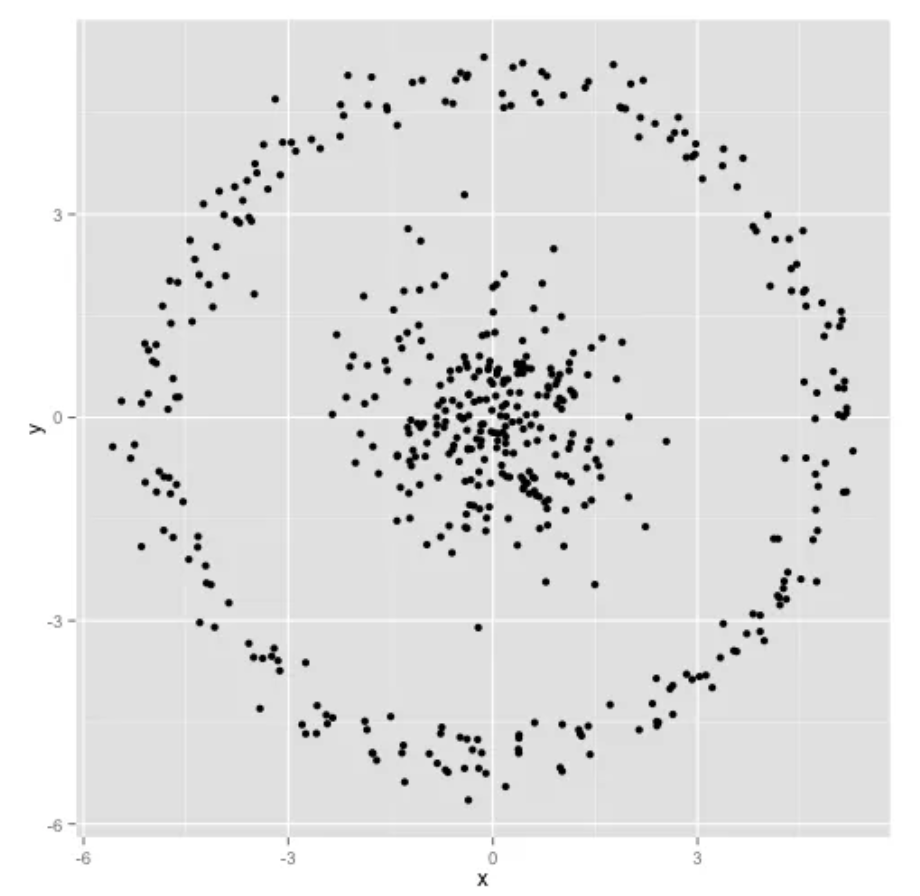
\includegraphics[width=0.4\columnwidth]{img/k-means-example.png}
            \caption{K means example}
            \label{fig:k-means-example}
        \end{figure}
        
        \begin{answer}
            K-means is good at finding the clusters when they have spherical shapes. In this example only one of the cluster is of spherical shape, meaning that k-means will likely result in a failure mode regarding what a human would consider to be the natural clusters. Given that we set $k=2$, depending on initialization, we could end up with something along the lines of Figure \ref{fig:k-means-possible-sol}.

            \begin{figure}[h!]
                \centering
                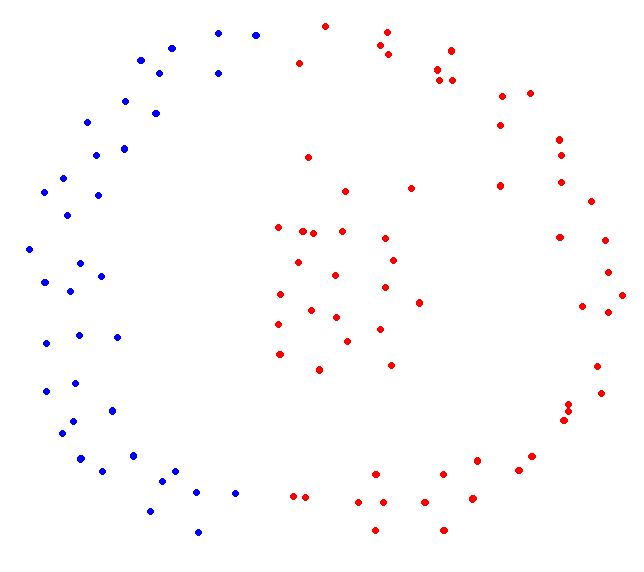
\includegraphics[width=0.4\columnwidth]{img/k-means-possible-sol.png}
                \caption{K means possible output}
                \label{fig:k-means-possible-sol}
            \end{figure}
            (See more \href{https://towardsdatascience.com/k-means-clustering-algorithm-applications-evaluation-methods-and-drawbacks-aa03e644b48a}{here}.)
        \end{answer}
    \end{InnerQandA}

    \item k-nearest neighbor classification.
    \begin{InnerQandA}
        \item How would you choose the value of k?
        \begin{answer}
            A good idea is to start with $k = \sqrt{N}$, where $N$ is the number of data points, and use Cross-Validation with (coarse-to-fine) grid search around the initial value to determine the best one for the dataset.
        \end{answer}

        \item What happens when you increase or decrease the value of k?
        \begin{answer}
            A small value of k can result in noise having too much influence on the result. A large value of k can make inference computationally expensive; moreover, it defeats the basic philosophy behind kNN that points that are near might have similar densities/classes.  

            (Source: \href{https://stackoverflow.com/questions/11568897/value-of-k-in-k-nearest-neighbor-algorithm}{StackOverflow})
        \end{answer}

        \item How does the value of k impact the bias and variance?
        \begin{answer}
            Using lower $k$ allows for more flexibility, therefore low bias, but high variance (different draws result in differently learned functions).\\\\
            On the other hand, using higher $k$ results in less flexibility, therefore high bias, but low variance (different draws don't result in differently learned functions).
        
            (Source: \href{https://stats.stackexchange.com/questions/485884/bias-and-variance-in-knn-and-decision-trees}{StackExchange})
        \end{answer}
    \end{InnerQandA}

    \item k-means and GMM are both powerful clustering algorithms.
    \begin{InnerQandA}
        \item Compare the two.
        \begin{answer}
            K-means is a clustering algorithm that uses the Euclidean distance to measure similarity. Given input data $X \in \R^{N \times F}$ (i.i.d. samples) and predefined number of clusters $K$, K-means outputs a set of clusters $\{V_1, V_2, \ldots, V_K\}$ s.t.:
            \begin{align*}
                \bigcup_{i=1}^K V_i = X \quad\quad \forall i, j\neq i:  V_i \cap V_j = \emptyset
            \end{align*}
            It does so by minimizing the following objective function:
            \begin{align*}
                \min_{\mu, z} \sum_{n=1}^N \sum_{k=1}^K z_{nk} \Vert \mu_k - x_n \Vert^2
            \end{align*}
            where $\mu_k \in \R^{F}$ is the centroid of cluster $k$, and $z$ is an assignment matrix s.t.:
            \begin{align*}
                z_{nk} = \begin{cases}
                    1 & \text{if } x_n \in V_k \\
                    0 & \text{otherwise}
                \end{cases}
            \end{align*}
            K-means minimizes the aforementioned objective by first initializing $\mu_k$ for all $k$, and then iterating between:
            \begin{enumerate}[label=\arabic*.]
            \item \textit{Assign step.} For all $n$, compute $z_{n}$ (given $\mu$):
            \begin{align*}
                z_{nk} = \begin{cases}
                    1 &\text{if } k = \argmin_{j} \Vert x_n - \mu_j \Vert^2_2 \\
                    0 &\text{otherwise}
                \end{cases}
            \end{align*}
            \item \textit{Update step.} For all $k$, compute $\mu_k$ (given $z$):
            \begin{align*}
                \mu_K = \frac{\sum_{n=1}^N z_{nk} x_n}{\sum_{n=1}^N z_{nk}}
            \end{align*}
            \end{enumerate}
            We terminate the algorithm when assignments do not change anymore. Convergence to a local optimum is guaranteed since each assign step decreases the cost. Convergence to a globally optimal solution is not guaranteed. \\\\
            Interestingly, we can arrive at the above-mentioned optimization objective from the maximum likelihood principle, by assuming that the data is i.i.d, and that the clusters correspond to a Gaussian distribution with mean $\mu_k$ and $I$ (identity) covariance matrix (resulting in spherical clusters):
            \begin{align*}
                p(x_n \g z, \mu) &= \prod_{k=1}^K \left[ \mathcal{N}(x_n \g \mu_k, I) \right]^{z_{nk}}\\
                \implies p(X \g z, \mu) &= \prod_{n=1}^N \prod_{k=1}^K \left[ \mathcal{N}(x_n \g \mu_k, I) \right]^{z_{nk}} \\
                \implies -\log(p(X \g z, \mu)) &= - \sum_{n=1}^N\sum_{k=1}^K z_{nk} \Vert x_n - \mu_k \Vert^2_2
            \end{align*}
            By diving in this probabilistic interpretation of K-means, we discover its issues:
            \begin{itemize}
                \item All clusters have spherical shapes.
                \item Each point can belong to only one cluster.
            \end{itemize}
            Gaussian Mixture Models (GMM) address these two limitations:
            \begin{itemize}
                \item Clusters do not have to be spherical: covariance matrix of Gaussian distribution is full-covariance $\Sigma$ not $I$.
                \item Samples can belong to more than one cluster (soft clustering) by fractional assignment which is interpreted as probabilities.
            \end{itemize}
            GMMs characterize the data by:
            \begin{itemize}
                \item Means $\{\mu_k\}_{k=1}^K$ 
                \item Covariance matrices $\{\Sigma_k\}_{k=1}^K$ 
                \item Weights of the Gaussians $\{\pi_k\}_{k=1}^K$
            \end{itemize}
            \begin{align*}
                \theta := \{\{\mu_k\}_{k=1}^K, \{\Sigma_k\}_{k=1}^K, \{\pi_k\}_{k=1}^K\}
            \end{align*}
            With that, they represent the data as a mixture of densities:
            \begin{align*}
                p(x_n \g \theta) = \sum_{k=1}^K \pi_k \mathcal{N} (x_n \g \mu_k, \Sigma_k)
            \end{align*}
            Similar as before, the goal is to find $\theta$ that maximizes the log-likelihood for the data $X$:
            \begin{align*}
                \log(p(X \g \theta)) = \sum_{n=1}^N \log \sum_{k=1}^K \mathcal{N} (x_n \g \mu_k, \Sigma_k)
            \end{align*}
            However, finding an analytical expression that directly maximizes the log-likelihood is hard, since we cannot push the log inside the sum. For this reason, we turn to an iterative technique called Expectation Maximization (EM), which consists of two steps:
            \begin{itemize}
                \item \textit{E-step:} missing data are estimated given observed data and current estimate of the parameters.
                \item \textit{M-step:} likelihood function is maximized under the assumption that the missing data are known.
            \end{itemize}
            EM is guaranteed to increase the likelihood at each iteration, although might end in a local optimum.\\\\
            Going back to our clustering problem, let us expand the posterior probability that a sample $n$ belongs to a cluster $k$ (which is in fact, the optimal cluster assignment):
            \begin{align*}
                q_{nk} := p(z_n = k \g x_n, \theta) &= \frac{p(z_n = k, x_n, \theta)}{p(x_n, \theta)} \\
                &= \frac{p(z_n = k, x_n \g \theta)}{p(x_n \g \theta)} \\
                &= \frac{p(z_n = k, x_n \g \theta)}{\sum_{j=1}^K p(z_j, x_n \g \theta)} \\
                &= \frac{p(z_n=k \g \theta)p(x_n \g z_n = k, \theta)}{\sum_{j=1}^K p(z_n=j \g \theta)p(x_n \g z_n = j, \theta)} \\
                &= \frac{\pi_k \mathcal{N}(x_n \g \mu_k, \Sigma_k)}{\sum_{j=1}^K \pi_j \mathcal{N}(x_n \g \mu_j, \Sigma_j)}
            \end{align*}
            So, if we know $\mu$, $\Sigma$ and $\pi$, we have a closed form solution for the posterior $q$. \\\\
            On the other hand, by computing a derivative of the log-likelihood mentioned above, and setting it to zero, we obtain the optimal parameters for $\mu$, $\Sigma$ and $\pi$:
            \begin{align*}
                \mu_k &= \frac{\sum_{n=1}^N q_{nk} x_n}{\sum_{n=1}^N q_{nk}}\\
                \Sigma_k &= \frac{\sum_{n=1}^N q_{nk}(x_n - \mu_k)(x_n - \mu_k)^T}{\sum_{n=1}^N q_{nk}} \\
                \pi_k &= \frac{1}{N}\sum_{n=1}^N q_{nk}
            \end{align*}
            However, this requires us to know the optimal $q$. Therefore, we are in a chicken-and-egg type problem: we need $\mu, \Sigma, \pi$ to estimate the posterior cluster assignments $q_{nk}$; but also we need $q_{nk}$ in order to estimate $\mu, \Sigma, \pi$. \\\\
            This leads us to the iterative EM solution for the GMM algorithm. At time $t$ perform:
            \begin{enumerate}[label=\arabic*.]
                \item E-step (assign): compute cluster assignments (given current estimate of $\theta$):
                \begin{align*}
                    q_{nk}^t = \frac{\pi_k^t \mathcal{N}(x_n \g \mu_k^t, \Sigma_k^t)}{\sum_{j=1}^K \pi_j^t \mathcal{N}(x_n \g \mu_j^t, \Sigma_j^t)}
                \end{align*}
                \item M-Step (update): update the cluster parameters $\mu_k^{t+1}, \Sigma_{k}^{t+1}, \pi_k^{t+1}$
                \begin{align*}
                \mu_k^{t+1} &= \frac{\sum_{n=1}^N q_{nk}^t x_n}{\sum_{n=1}^N q_{nk}^t}\\
                \Sigma_k^{t+1} &= \frac{\sum_{n=1}^N q_{nk}^t(x_n - \mu_k^{t+1})(x_n - \mu_k^{t+1})^T}{\sum_{n=1}^N q_{nk}^t} \\
                \pi_k^{t+1} &= \frac{1}{N}\sum_{n=1}^N q_{nk}^t
            \end{align*}
            \end{enumerate}

            (Source: \href{https://www.youtube.com/watch?v=4FG0TWJRRPI&ab_channel=CarletonAISociety}{CAIS})
        \end{answer}

        \item When would you choose one over another?
        \begin{answer}
            In general case, it would be advisable to default to using GMMs, since they generalize better to various cluster shapes. However, given some prior knowledge that the clusters are supposed to have spherical shapes, it might be beneficial to use K-Means as it explicitly encodes this property.
        \end{answer}
    \end{InnerQandA}

    \item Bagging and boosting are two popular ensembling methods. Random forest is a bagging example while XGBoost is a boosting example.
    \begin{InnerQandA}
        \item What are some of the fundamental differences between bagging and boosting algorithms?
        \begin{answer}
            With bagging, instead of training one model on the entire dataset, we sample with replacement to create several different datasets, and train a separate model on each of the bootstraps. Sampling with replacement ensures each bootstrap is independent of its peers. \\\\
            In contrast, with boosting we train several models iteratively (one by one) on the entire dataset. However, after training a model, we adjust each sample's weight based on the current ensemble performance, and train the next model on the re-weighted dataset.\\\\
            With that said, the fundamental differences between bagging and boosting are:
            \begin{itemize}
                \item Bagging can train all models in parallel (fast), but each one of them is independent of how well the others are doing. 
                \item Boosting trains the models iteratively (slow), but each next model learns from the mistakes of the previous ones.
            \end{itemize}
        \end{answer}

        \item How are they used in deep learning?
        \begin{answer}
            While in theory there is nothing stopping you from applying bagging and boosting to deep neural networks, in practice it is almost infeasible. \\\\
            Historically, these ensembling techniques have been introduced by combining many weak (slightly above random performance), but inexpensive learners such as decision trees. \\\\
            Today, deep neural networks are so large that even a single model is distributed among many nodes for distributed training. To consider training hundreds of networks for the purposes of boosting/bagging is almost unimaginable. Even if we somehow train them, at inference time the predictions can take from seconds to several minutes, deeming them extremely impractical (e.g. self-driving cars). \\\\
            Moreover, it is known that neural networks are very sample inefficient, requiring huge datasets which can take weeks to months to train on. This means that training in an iterative manner, such as in boosting, could take months to years to finish.
        \end{answer}
    \end{InnerQandA}

    \item Given this directed graph (see Figure \ref{fig:directed-graph}).
    \begin{figure}[htb!]
        \centering
        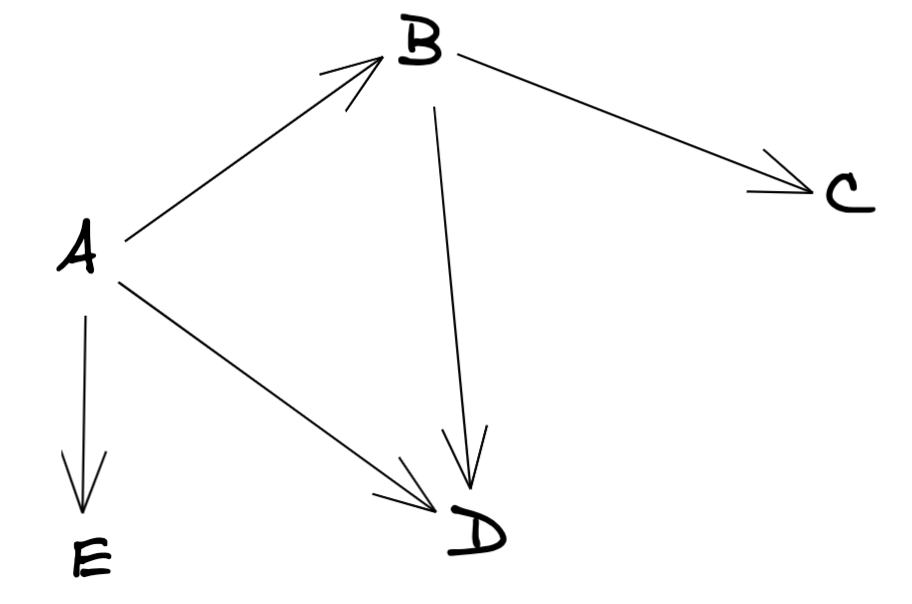
\includegraphics[width=0.3\columnwidth]{img/directed-graph.png}
        \caption{Example of a directed graph}
        \label{fig:directed-graph}
    \end{figure}
    \begin{InnerQandA}
        \item Construct its adjacency matrix.
        \begin{answer} 
            \begin{align*}
                \begin{bmatrix}
                    0 & 1 & 0 & 1 & 1 \\
                    0 & 0 & 1 & 1 & 0 \\
                    0 & 0 & 0 & 0 & 0 \\
                    0 & 0 & 0 & 0 & 0 \\
                    0 & 0 & 0 & 0 & 0
                \end{bmatrix}
            \end{align*}
            
        \end{answer}

        \item How would this matrix change if the graph is now undirected?
        \begin{answer}
            We add edges in the opposite direction as well, making the matrix symmetric:
            \begin{align*}
                \begin{bmatrix}
                    0 & 1 & 0 & 1 & 1 \\
                    1 & 0 & 1 & 1 & 0 \\
                    0 & 1 & 0 & 0 & 0 \\
                    1 & 1 & 0 & 0 & 0 \\
                    1 & 0 & 0 & 0 & 0
                \end{bmatrix}
            \end{align*}
        \end{answer}

        \item What can you say about the adjacency matrices of two isomorphic graphs?
        \begin{answer}
            Let us quickly note that the $(i, j)$-th entry of a matrix $M$ is equal to $e_i^T M e_j$, where $e_i$ is a vector with $1$ in the $i$-th entry and $0$ elsewhere. \\\\
            Let $G_A$ and $G_B$ be two isomorphic graphs, whose adjacency matrices are $A$ and $B$. Given that isomorphic graphs are identical up to a permutation $\pi$, we want the $(i, j)$-th entry of $A$ to be the same as the $(\pi(i), \pi(j))$-th entry of $B$:
            \begin{align*}
                e_i^T A e_j = (Pe_i)^T B (Pe_j) = e_i^T (P^T B P) e_j
            \end{align*}
            where $P$ is the matrix corresponding to the permutation $\pi$. For this to hold for all $i$ and $j$, we must have:
            \begin{align*}
                 A = P^T B P
            \end{align*}
            
            (Source: \href{https://math.stackexchange.com/questions/181273/graph-isomorphism-as-permutation-matrix}{StackExchange})
        \end{answer}
    \end{InnerQandA}

    \item Imagine we build a user-item collaborative filtering system to recommend to each user items similar to the items they’ve bought before.
    \begin{InnerQandA}
        \item You can build either a user-item matrix or an item-item matrix. What are the pros and cons of each approach?
        \begin{answer}
            \todo 
        \end{answer}

        \item How would you handle a new user who hasn’t made any purchases in the past?
        \begin{answer}
            \todo
        \end{answer}
    \end{InnerQandA}

    \item Is feature scaling necessary for kernel methods?
    \begin{answer}
        In general, feature scaling is important for kernel methods. The kernel is effectively a distance and if different features vary on different scales then this can matter. For instance, for the RBF kernel we have:
        \begin{align*}
            K(x, x') = \exp \left(-\gamma \left\Vert x - x'\right\Vert^2 \right)
        \end{align*}
        so if one dimension takes much larger values than others then it will dominate the kernel values and you'll lose some signal in other dimensions. This applies to the linear kernel too. \\\\
        Nevertheless, this doesn't apply to all kernels, since some have scaling built in. A typical example is the Mahalanobis kernel:
        \begin{align*}
            K(x, x') = \exp \left(-\gamma (x - x')^T\hat{\Sigma}^{-1}(x-x') \right)
        \end{align*}
        where $\hat{\Sigma}$ is the sample covariance matrix.

        (Source: \href{https://stats.stackexchange.com/questions/305906/feature-scaling-in-svm-does-it-depend-on-the-kernel}{StackExchange})
    \end{answer}

    \item Naive Bayes classifier.
    \begin{InnerQandA}
        \item How is Naive Bayes classifier naive?
        \begin{answer}
            Suppose we are performing classification, and want to determine the posterior proability for class $y$, given some input $x_1, \ldots, x_m$. Then, using Bayes' rule we would get:
            \begin{align*}
                p(y \g x_1, \ldots x_m) &= \frac{p(x_1, \ldots x_m \g y) p(y)}{p(x_1, \ldots, x_m)}
            \end{align*}
            Naive Bayes is naive since it assumes conditional independence of the observations $x_i$ given the class $y$:
            \begin{align*}
                p(y \g x_1, \ldots x_m) &= \frac{p(x_1, \ldots x_m \g y) p(y)}{p(x_1, \ldots, x_m)} \underbrace{=}_{\text{naive}} \frac{p(x_1 \g y) \hdots p(x_m \g y) p(y)}{p(x_1, \ldots, x_m)}
            \end{align*} 
            Since we are typically only interested in comparing the unnormalized scores for the various classes, notice that we can disregard the evidence term in the denominator:
            \begin{align*}
                p(y \g x_1, \ldots x_m) \propto p(x_1 \g y) \hdots p(x_m \g y) p(y)
            \end{align*}
            Lastly, if we are performing text classification, and certain words are missing from the corpora for the given class, notice that the entire product will result in $0$, since $p(x_i \g y) = 0$. In this case, it is a good idea to perform Laplace smoothing, by adding a pseudocount of 1 for each word.
        \end{answer}

        \item Let’s try to construct a Naive Bayes classifier to classify whether a tweet has a positive or negative sentiment. We have four training samples (see Table \ref{tab:naive-bayes}). According to your classifier, what's sentiment of the sentence ``The hamster is upset with the puppy''?
        \begin{table}[h!]
        \centering
        \begin{tabular}{|l|l|}
        \hline
        \textbf{Tweet}                  & \textbf{Label} \\ \hline
        This makes me so upset          & Negative       \\ \hline
        This puppy makes me happy       & Positive       \\ \hline
        Look at this happy hamster      & Positive       \\ \hline
        No hamsters allowed in my house & Negative       \\ \hline
        \end{tabular}
        \caption{Naive Bayes example}
        \label{tab:naive-bayes}
        \end{table}
        
        \begin{answer}
        In order to improve the robustness of Naive Bayes, it is a good idea to transform all words to lowercase, remove stop words, and perform \href{https://www.geeksforgeeks.org/python-stemming-words-with-nltk/}{word stemming} (remove plural form of nouns, tense of verbs, etc.). After pre-processing the inputs, our resulting dataset is illustrated in Table \ref{tab:naive-bayes-transformed-dataset}. 
        
        \begin{table}[h!]
        \centering
        \begin{tabular}{|l|l|}
        \hline
        \textbf{Tweet}         & \textbf{Label} \\ \hline
        make upset             & Negative       \\ \hline
        puppy make happy       & Positive       \\ \hline
        look happy hamster     & Positive       \\ \hline
        hamster allow house & Negative       \\ \hline
        \end{tabular}
        \caption{Naive Bayes transformed dataset}
        \label{tab:naive-bayes-transformed-dataset}
        \end{table}
        
        Moreover, the pre-processed input which we wish to classify becomes ``hamster upset puppy''. Lastly, notice that some of the words in the input sentence don't exist for one of the classes (e.g. upset is not present for the positive class); therefore, we will perform Laplace smoothing by adding a pseudocount of 1 for all words in the corpus. \\
        With that said, we specify the counts of each word given that they appear in the positive/negative tweets (accounted for Laplace smoothing) in Table \ref{tab:word-counts}.\\

        \begin{table}[h!]
        \centering
        \begin{tabular}{|c|c|c|}
        \hline
        \textbf{word}  & \textbf{positive count} & \textbf{negative count} \\ \hline
        mouse          & 2                       & 2                       \\ \hline
        upset          & 1                       & 2                       \\ \hline
        puppy          & 2                       & 1                       \\ \hline
        happy          & 3                       & 1                       \\ \hline
        look           & 2                       & 1                       \\ \hline
        hamster        & 2                       & 2                       \\ \hline
        allow          & 1                       & 2                       \\ \hline
        house          & 1                       & 2                       \\ \hline \hline
        \textbf{total} & 14                      & 13                      \\ \hline
        \end{tabular}
        \caption{Word counts}
        \label{tab:word-counts}
        \end{table}
        Finally, let us calculate the scores for the positive and negative class:
        \begin{align*}
            p(\text{Positive} \g \text{hamster upset puppy}) &\propto p(\text{hamster} \g \text{Positive}) p(\text{upset} \g \text{Positive}) p(\text{puppy} \g \text{Positive}) p(\text{Positive})\\
            &= \frac{2}{14} \cdot \frac{1}{14} \cdot \frac{2}{14} \cdot \frac{1}{2} = 0.00072\\\\
            p(\text{Negative} \g \text{hamster upset puppy}) &\propto p(\text{hamster} \g \text{Negative}) p(\text{upset} \g \text{Negative}) p(\text{puppy} \g \text{Negative}) p(\text{Negative})\\
            &= \frac{2}{13} \cdot \frac{2}{13} \cdot \frac{2}{13} \cdot \frac{1}{2} = 0.00091
        \end{align*}
        We conclude that the sentiment of the tweet is negative.

        (See more \href{https://www.youtube.com/watch?v=O2L2Uv9pdDA&ab_channel=StatQuestwithJoshStarmer}{here})
        \end{answer}
    \end{InnerQandA}

    \item Two popular algorithms for winning Kaggle solutions are Light GBM and XGBoost. They are both gradient boosting algorithms.
    \begin{InnerQandA}
        \item What is gradient boosting?
        \begin{answer}
            Gradient boosting is an idea that combines the techniques of gradient descent and boosting. \\\\
            The idea is to fit an ensemble $\sum_t \rho_t h_t(x)$ in stage-wise manner, where in each stage we introduce a weak learner to compensate the shortcomings of existing weak learners. In contrast to Adaboost which identifies shortcomings by high-weight data points, Gradient Boosting identifies shortcomings by gradients.\\\\
            To illustrate Gradient Boosting, suppose we are doing least-squares regression, where the goal is to teach a model $F$ to predict values of the form $\hat{y} = F(x_i)$ by minimizing the mean squared error:
            \begin{align*}
                L(y, \hat{y}) = \frac{1}{2n}\sum_{i=1}^n (\hat{y_i} - y_i)^2
            \end{align*}
            In gradient boosting, we approach this problem by building the final model in $M$ stages. At each stage $m$ ($1 \le m \le M$), suppose we have some imperfect model $F_m$ which we wish to improve by adding a new estimator $h_m$ as follows:
            \begin{align*}
                F_{m+1}(x_i) := F_m(x_i) + h_m(x_i) = y_i 
            \end{align*}
            or equivalently:
            \begin{align*}
                h_m(x_i) = y_i - F_m(x_i)
            \end{align*}
            Therefore, we will fit $h_m$ to the residuals $y_i - F_m(x_i)$. \\\\
            Now, let us see how this algorithm is related to gradient descent. Recall that when training neural nets, we minimize the objective by moving in the opposite direction of the gradient of the loss wrt. the \textit{parameters}:
            \begin{align*}
                \theta^{t+1} := \theta^t - \frac{\partial L}{\partial \theta^t}
            \end{align*}
            In contrast, in Gradient Boosting we minimize the loss by instead adjusting the \textit{outputs} $F(x_i)$ for each sample $x_i$. In other words, we treat $F(x_i)$ as parameters and take derivatives:
            \begin{align*}
                \frac{\partial L}{\partial F(x_i)} = \frac{\partial \sum_i L(y_i, F(x_i))}{\partial F(x_i)} = \frac{\partial L(y_i, F(x_i))}{\partial F(x_i)} = F(x_i) - y_i = - h(x_i)
            \end{align*}
            Therefore, we can interpret the residuals as the negative gradients:
            \begin{align*}
                h(x_i) = y_i - F(x_i) = - \frac{\partial L}{\partial F(x_i)}
            \end{align*}
            Finally, notice how the improvement step of our current estimator resembles the gradient descent update in neural nets:
            \begin{align*}
                F_{m+1}(x_i) &:= F_m(x_i) + h_m(x_i) \\
                \Leftrightarrow F_{m+1}(x_i) &:= F_m(x_i) + (-\frac{\partial L}{\partial F_m(x_i)}) \\
                \Leftrightarrow F_{m+1}(x_i) &:= F_m(x_i) 
                - 1 \cdot \frac{\partial L}{\partial F_m(x_i)}
            \end{align*}
            This means that we are in fact updating our model with gradient descent! \\\\
            It turns out that performing the update with gradients, instead of fitting the residual, is more general and useful. In short, we can theoretically plug in any differentiable function for $L$, and inject its properties when fitting the next model. For example, we can utilize the \href{https://en.wikipedia.org/wiki/Huber_loss}{Huber loss} which is more robust to outliers:
            \begin{align*}
                L(y, \hat{y}) = \begin{cases}
                    \frac{1}{2}(\hat{y} - y)^2 &\text{if } \vert \hat{y} - y \vert \le \delta \\
                    \delta(\vert \hat{y} - y \vert - \delta/2) &\text{otherwise}
                \end{cases}
            \end{align*}
            (Source: \href{http://www.chengli.io/tutorials/gradient_boosting.pdf}{Cheng Li's slides}, \href{https://en.wikipedia.org/wiki/Gradient_boosting}{Wikipedia})
            
        \end{answer}

        \item What problems is gradient boosting good for?
        \begin{answer}
            Gradient Boosting is most useful with tabular/structured data, where interpretability is not required, and there are no strict latency constraints for model prediction time.
        \end{answer}
    \end{InnerQandA}

    \item SVM.
    \begin{InnerQandA}
        \item What’s linear separation? Why is it desirable when we use SVM?
        \begin{answer}
            Two sets are linearly separable if there exists at least one hyperplane that splits the space in such a way that all of the points of the first set lie on one one side of the hyperplane, and all of the points of the second set lie on the other side. \\\\
            In the linearly separable case, SVM is trying to find the hyperplane that maximizes the margin, with the condition that both classes are classified correctly. But in reality, datasets are almost never linearly separable, so the condition of 100\% correctly classified by a hyperplane will never be met.\\\\
            SVM address non-linearly separable cases by introducing two techniques:
            \begin{itemize}
                \item \textit{Soft Margin}: try to find a linear decision boundary, but tolerate a few misclassified samples;
                \item \textit{Kernel Trick}: try to find a non-linear decision boundary.
            \end{itemize}

            (Source: \href{https://towardsdatascience.com/support-vector-machine-simply-explained-fee28eba5496}{TowardsDataScience})
        \end{answer}

        \item How well would vanilla SVM work on this dataset (see Figure \ref{fig:svm-example-1})?
        \begin{figure}[htb!]
            \centering
            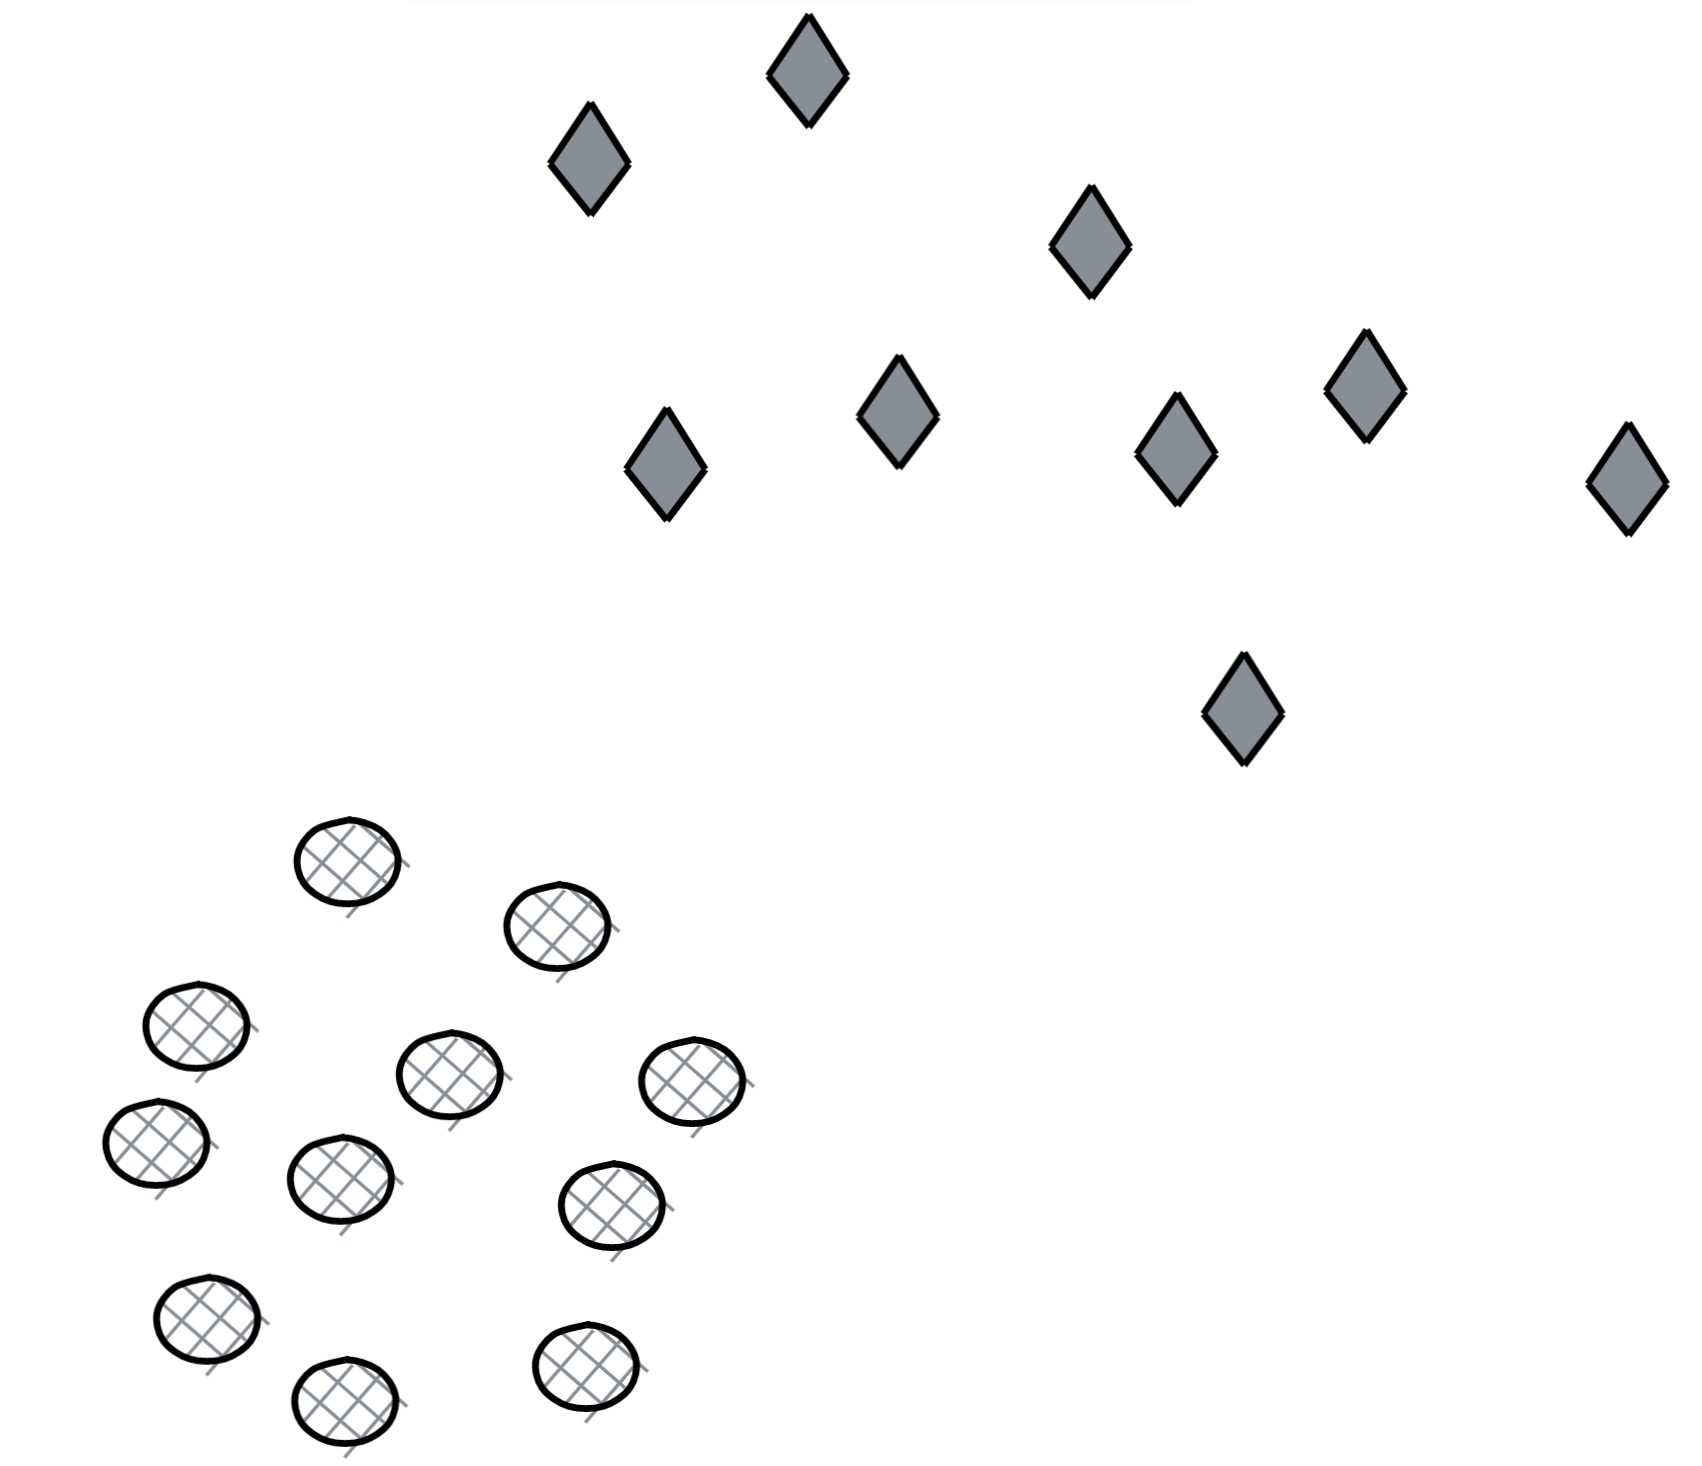
\includegraphics[width=0.3\columnwidth]{img/svm-example-1.png}
            \caption{SVM example 1}
            \label{fig:svm-example-1}
        \end{figure}
        \begin{answer}
            SVM would work as intended, by finding a linear decision boundary that maximizes the margin between the two classes (see Figure \ref{fig:-sol-svm-example-1}).
            \begin{figure}[htb!]
                \centering
                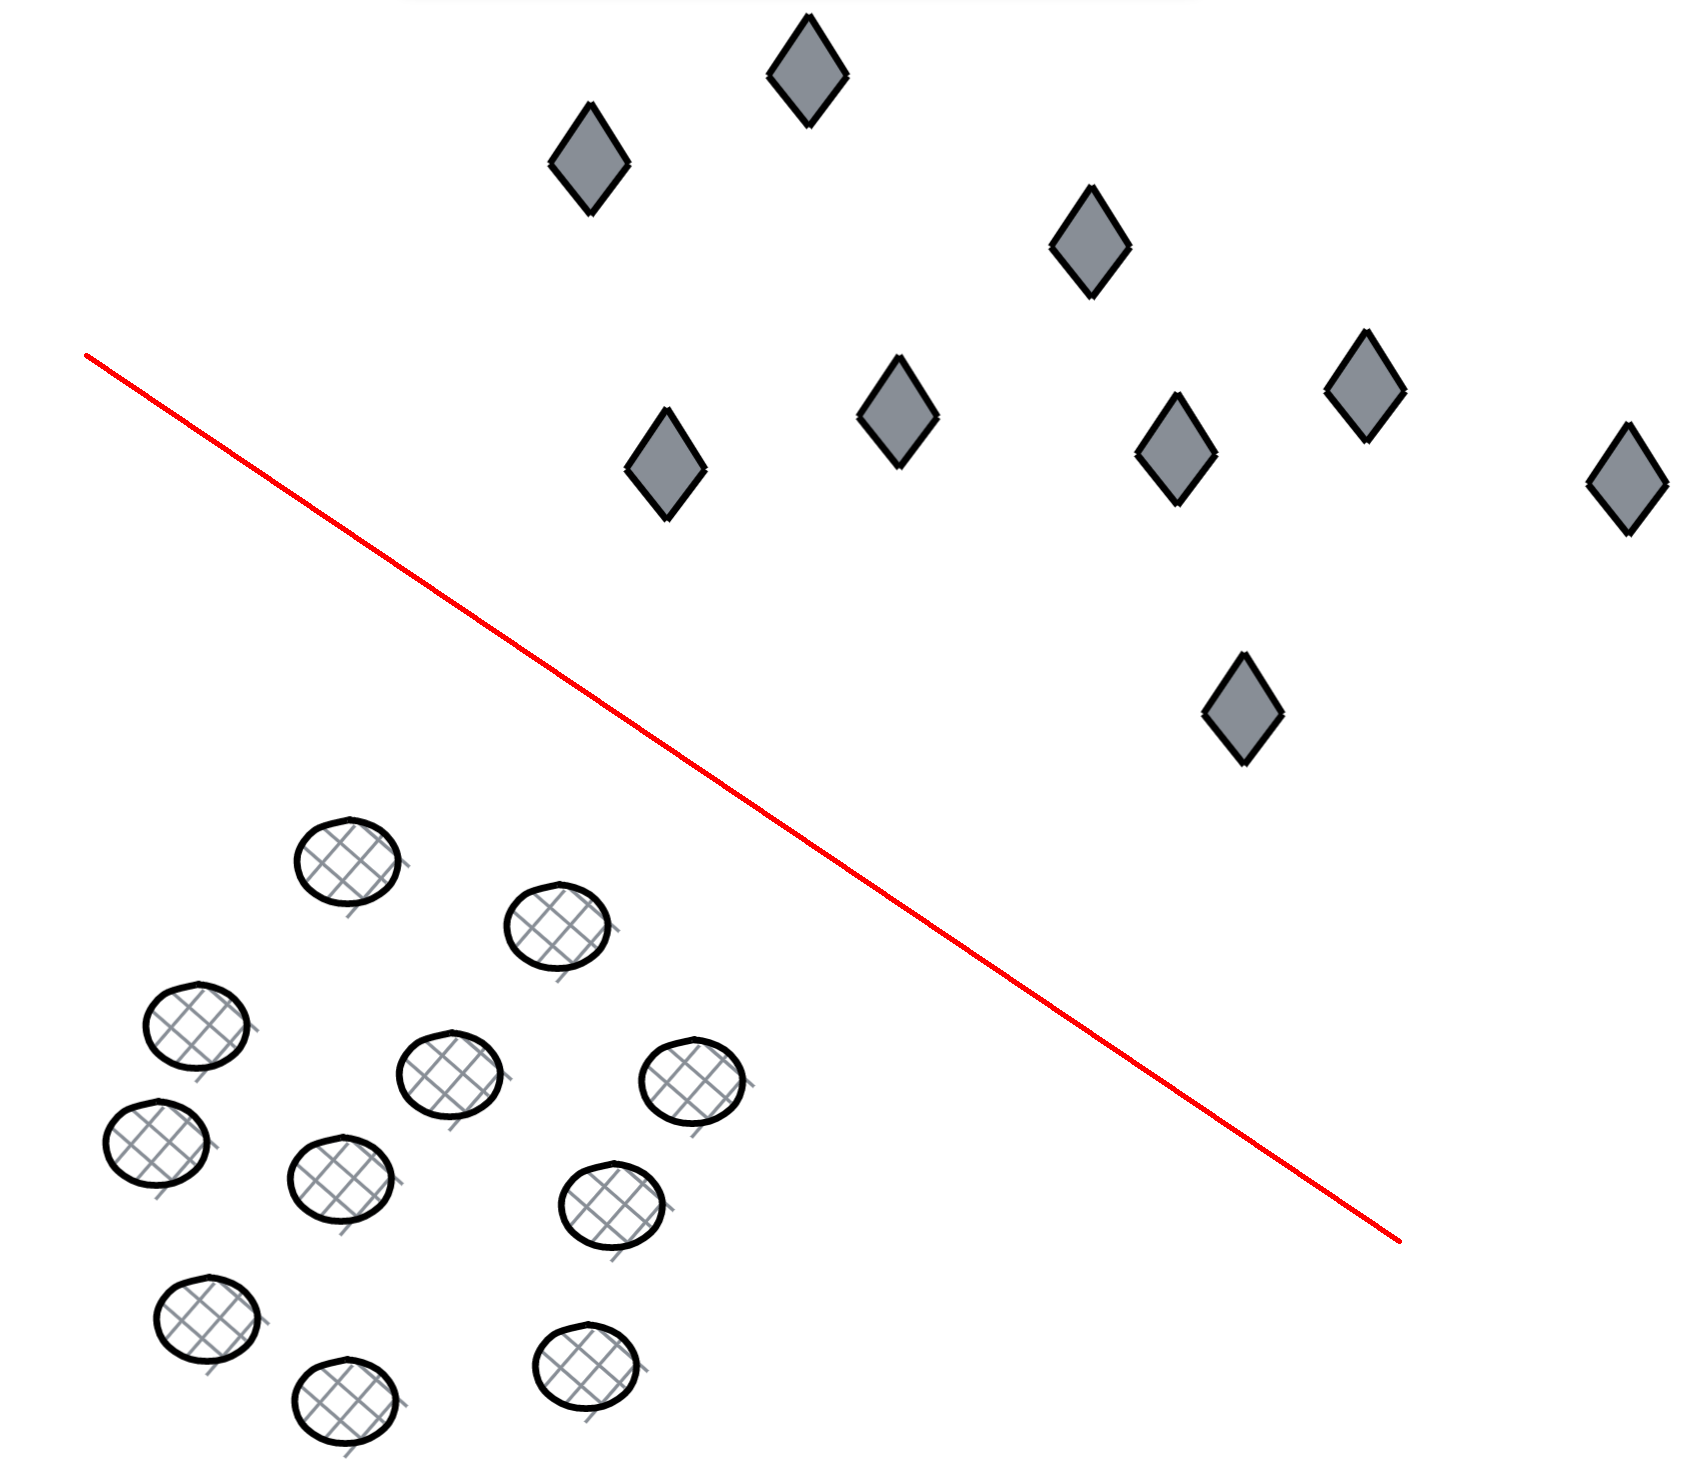
\includegraphics[width=0.3\columnwidth]{img/sol-svm-example-1.png}
                \caption{Solution to SVM example 1}
                \label{fig:-sol-svm-example-1}
            \end{figure}
        \end{answer}

        \item How well would vanilla SVM work on this dataset (see Figure \ref{fig:svm-example-2})?
        \begin{figure}[htb!]
            \centering
            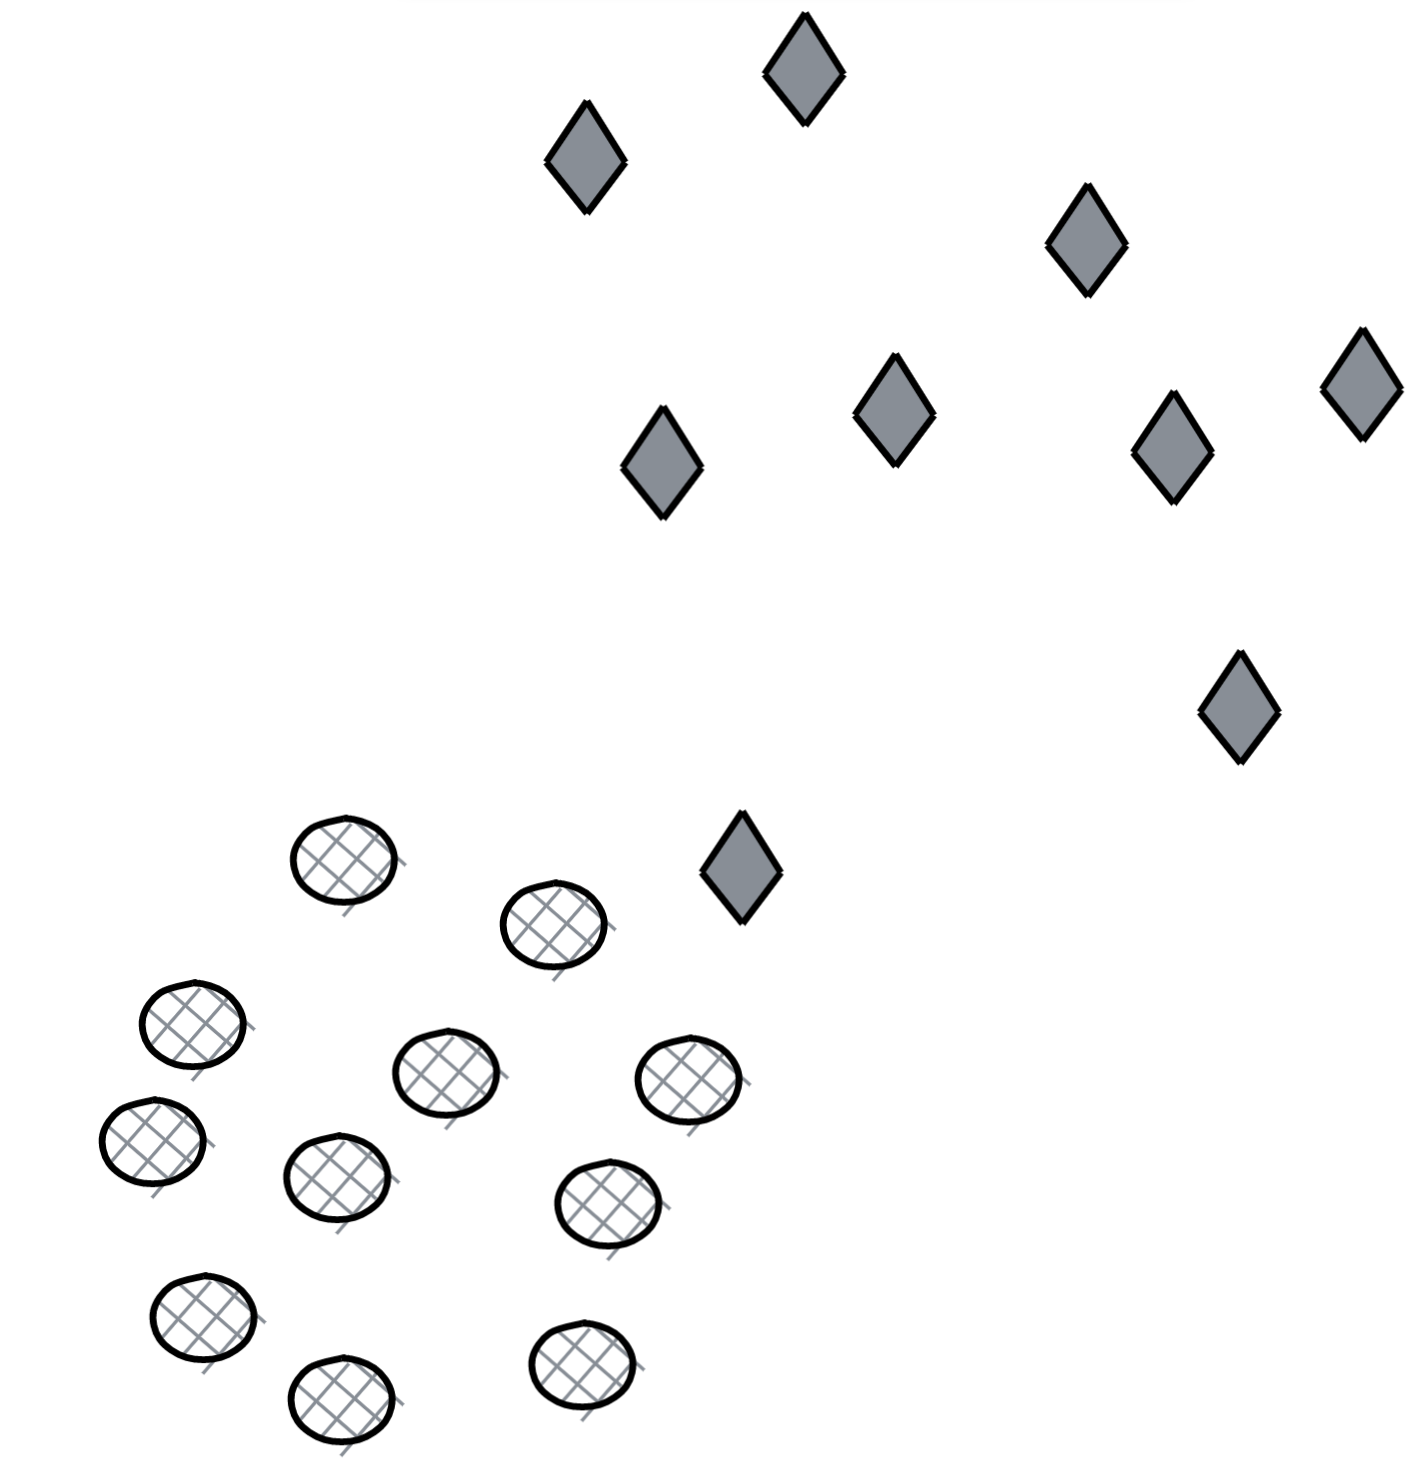
\includegraphics[width=0.3\columnwidth]{img/svm-example-2.png}
            \caption{SVM example 2}
            \label{fig:svm-example-2}
        \end{figure}
        \begin{answer}
            Again, SVM will still find a linear decision boundary that classifies all samples correctly. However, since we don't allow for any slackness, due to the one outlier, the boundary is more slanted compared to the previous one (see Figure \ref{fig:-sol-svm-example-2}). 
            \begin{figure}[htb!]
                \centering
                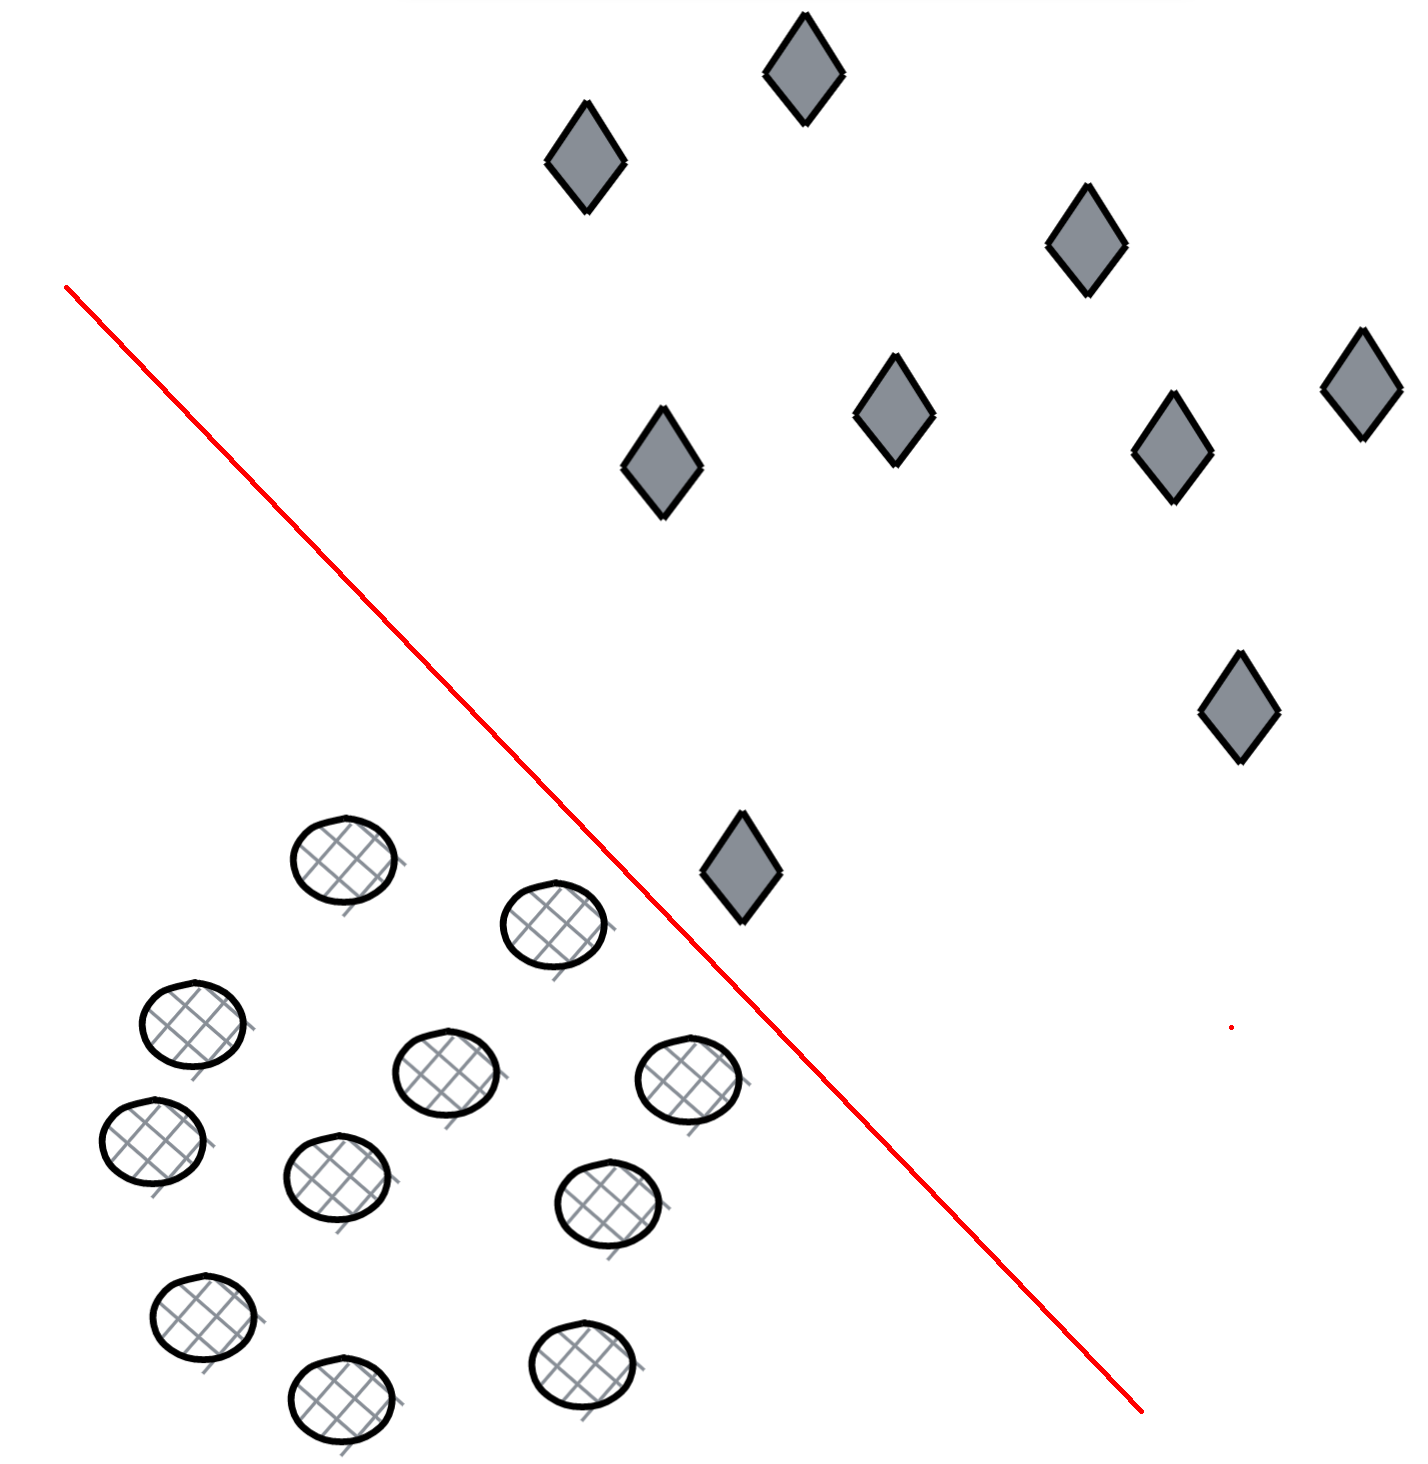
\includegraphics[width=0.3\columnwidth]{img/sol-svm-example-2.png}
                \caption{Solution to SVM example 2}
                \label{fig:-sol-svm-example-2}
            \end{figure}
        \end{answer}

        \item How well would vanilla SVM work on this dataset (see Figure \ref{fig:svm-example-3})?
        \begin{figure}[htb!]
            \centering
            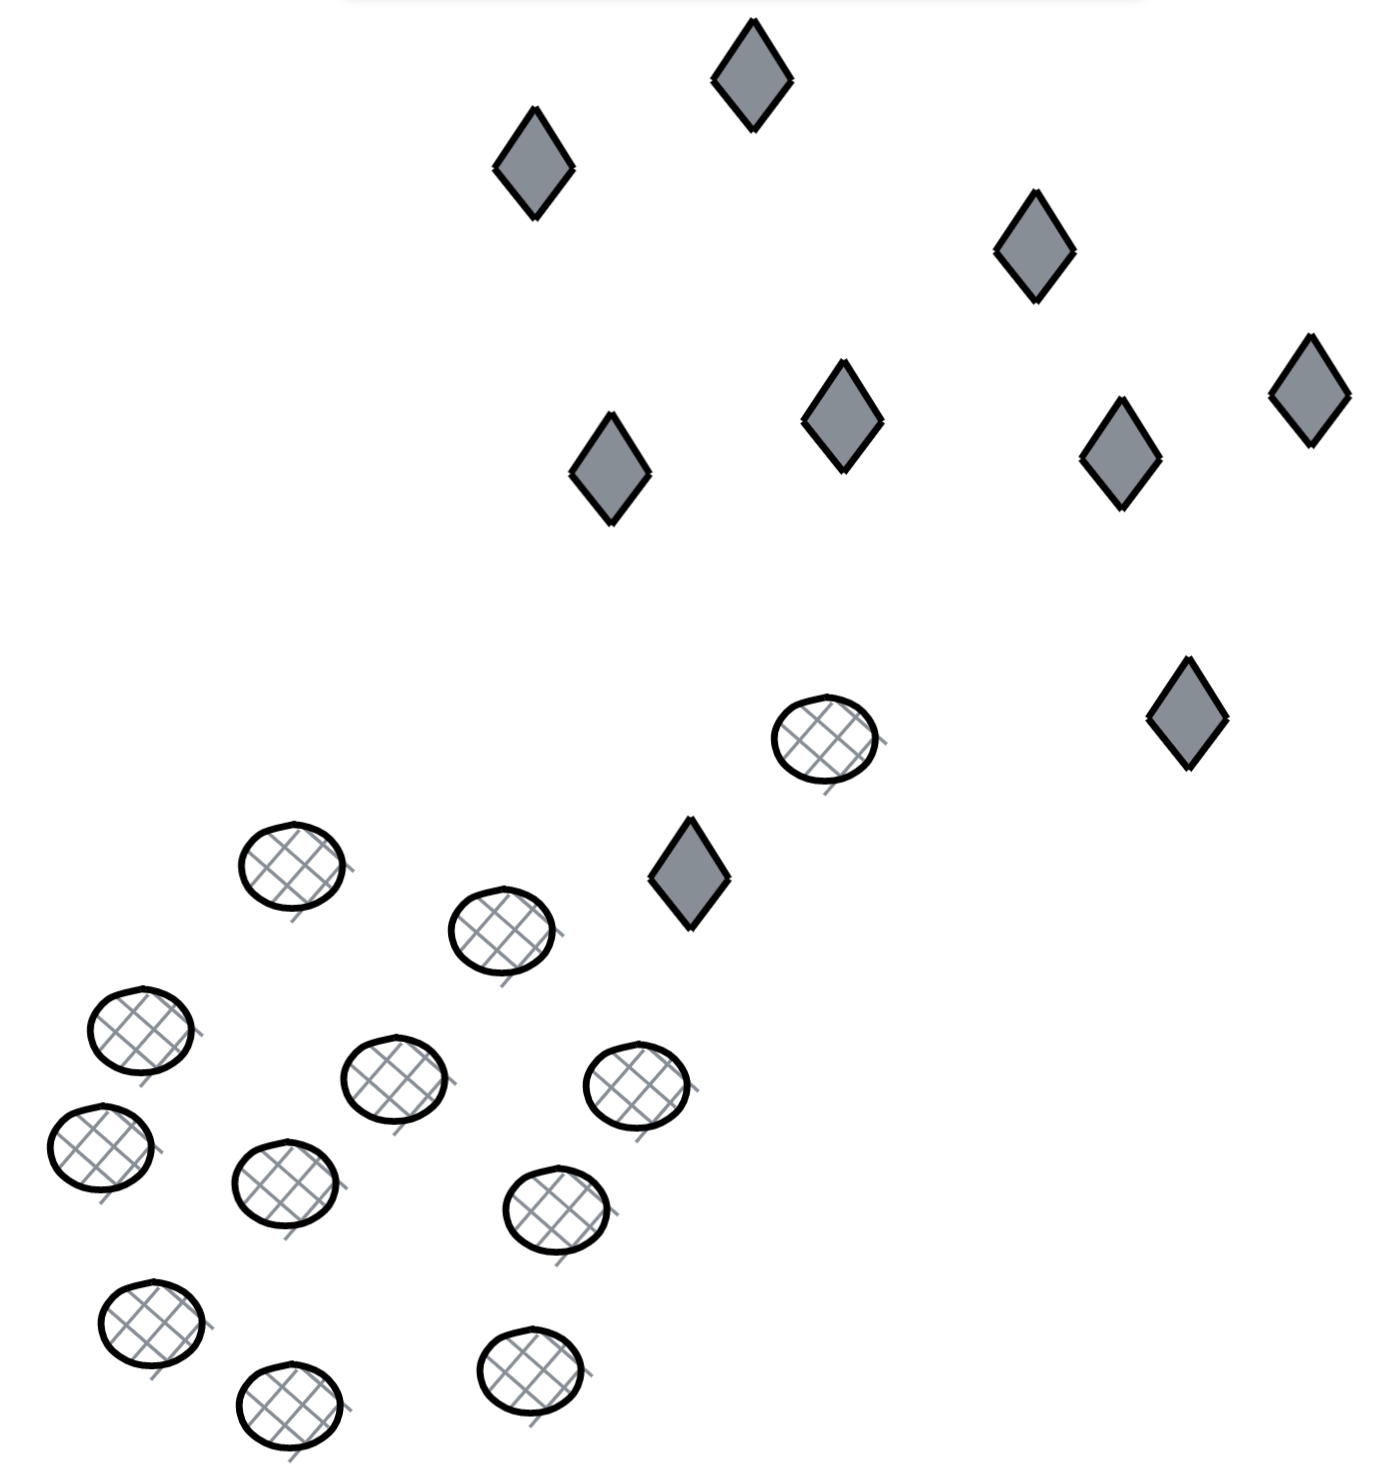
\includegraphics[width=0.3\columnwidth]{img/svm-example-3.png}
            \caption{SVM example 3}
            \label{fig:svm-example-3}
        \end{figure}
        \begin{answer}
            SVM won't work at all, since the two classes are not linearly separable. As discussed above, two potential solutions are: introducing slack variables; using non-linear kernels.
        \end{answer}
    \end{InnerQandA}
    
\end{QandA}

\subsection{Natural Language Processing}
\begin{QandA}
    \item RNNs
    \begin{InnerQandA}
        \item What’s the motivation for RNN?
        \begin{answer}
            A recurrent neural network (RNN) is a class of artificial neural networks where connections between nodes can create a cycle, allowing output from some nodes to affect subsequent input to the same nodes. This allows it to exhibit temporal dynamic behavior. Derived from feedforward neural networks, RNNs can use their internal state (memory) to process variable length sequences of inputs. This makes them applicable to tasks such as unsegmented, connected handwriting recognition or speech recognition. Recurrent neural networks are theoretically Turing complete and can run arbitrary programs to process arbitrary sequences of inputs.

            (Source: \href{https://en.wikipedia.org/wiki/Recurrent_neural_network}{Wikipedia})
        \end{answer}
        
        \item What’s the motivation for LSTM?
        \begin{answer}
            In theory, classic (or "vanilla") RNNs can keep track of arbitrary long-term dependencies in the input sequences. The problem with vanilla RNNs is computational in nature: when training a vanilla RNN using back-propagation, the long-term gradients which are back-propagated can "vanish" (that is, they can tend to zero) or "explode" (that is, they can tend to infinity), because of the computations involved in the process, which use finite-precision numbers. RNNs using LSTM units partially solve the vanishing gradient problem, because LSTM units allow gradients to also flow unchanged. 

            (Source: \href{https://en.wikipedia.org/wiki/Long_short-term_memory}{Wikipedia})
        \end{answer}
        
        \item How would you do dropouts in an RNN?
        \begin{answer}
            There are several possibilities for doing dropouts in RNNs:
            \begin{itemize}
                \item \textit{Dropout only to non-recurrent connections} -- thereby the network benefiting from regularization without sacrificing the memorization capabilities of the recurrent cells. 
                \item \textit{Variational Dropout} -- repeat the same dropout mask at each time step for both inputs, outputs and recurrent layers. 
                \item \textit{Recurrent Dropout} -- Apply dropout to the hidden state update vector, instead of the entire hidden state. 
                \item \textit{Zoneout} -- instead of setting some units’ activations to 0 as in dropout, zoneout randomly replaces some units’ activations with their activations from the previous timestep. This makes it easier for the network to preserve information from previous timesteps going forward, and facilitates, rather than hinders, the flow of gradient information going backward.
            \end{itemize}

            (See more \href{https://adriangcoder.medium.com/a-review-of-dropout-as-applied-to-rnns-72e79ecd5b7b}{here})
        \end{answer}

    \end{InnerQandA}
    \item What’s density estimation? Why do we say a language model is a density estimator?
        \begin{answer}
            In probability and statistics, density estimation is the construction of an estimate, based on observed data, of an unobservable underlying probability density function. The unobservable density function is thought of as the density according to which a large population is distributed; the data are usually thought of as a random sample from that population. \\\\
            On the other hand, a language model is a probability distribution over sequences of words. Given such a sequence of length m, a language model assigns a probability $P(w_1, \ldots, w_m)$ to the whole sequence. Language models generate probabilities by training on text corpora, which are considered random samples from the underlying population.

            (Source: \href{https://en.wikipedia.org/wiki/Density_estimation}{Wikipedia} \href{https://en.wikipedia.org/wiki/Language_model}{Wikipedia})
        \end{answer}
    

    \item Language models are often referred to as unsupervised learning, but some say its mechanism isn’t that different from supervised learning. What are your thoughts?
    \begin{answer}
        Language models are trained in a self-supervised manner, which can be considered an intersection point between supervised and unsupervised learning. By utilizing a large corpora of text scraped from the Internet without any labels (unsupervised learning), we mask out some words/tokens and train the model to predict the missing values (supervised learning, since we know the "ground-truth"). 
    \end{answer}

    \item Word embeddings.
    \begin{InnerQandA}
        \item Why do we need word embeddings?
        \begin{answer}
            Neural nets cannot handle textual features, so we have to transform them to numerical ones. However, simply enumerating the categories is plain wrong -- if you represent "apples" with 1, and "oranges" with 2, does it mean that "oranges" = 2 x "apples"? Another way to encode the categorical features is with one-hot encoding, but this can introduce data sparsity, which can be an undesired trait of our dataset as we have seen in a previous question. \\\\
            Therefore, one of the most widely used methods for encoding textual features is to use word embeddings, such as Word2Vec. The benefits of using an embedding is that it provides low-dimensional, distributed representation that allow for capturing relationships between the categories (eg. "king" - "man" + "woman" = "queen")
    
            (See more \href{https://www.fast.ai/2018/04/29/categorical-embeddings/}{here})
        \end{answer}

        \begin{figure}[ht!]
            \centering
            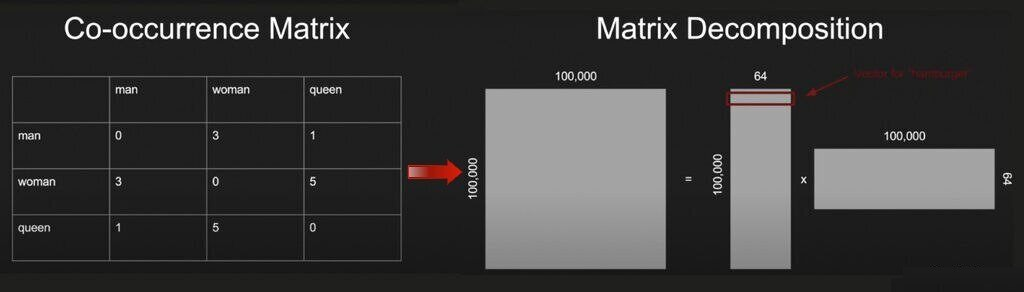
\includegraphics[width=0.8\columnwidth]{img/cooccurance.jpg}
            \caption{Count-based word embeddings}
            \label{fig:count-based-word-embeddings}
        \end{figure}

        \item What’s the difference between count-based and prediction-based word embeddings?
        \begin{answer}
            Words that appear in the same context or have semantic relevance have proximity in the vector representation. There are two different ways vectors are represented from text: count-based and predictive-based methods.\\\\
            \textit{Count-based word embeddings} start off by building a co-occurrence matrix, and then either use a matrix decomposition method (e.g. SVD, see Figure \ref{fig:count-based-word-embeddings}), or an algorithm based on gradient descent (e.g. GloVe) to extract the embeddings. The intuitive reason why matrix decomposition should work is that the correlation (or relative co-occurrence) of the words in the text corpora represented by the $(i,j)$-th entry in the co-occurrence matrix should be representable as a dot product (\href{https://www.quora.com/Is-there-any-relation-between-correlation-of-two-signals-and-dot-product-of-two-vectors}{covariance}) of the two embedding vectors. Similarly, GloVe optimizes for the dot products of pairs of embeddings (scaled by the co-occurrence), but instead using gradient descent to generate the vectors. \\
            
            % \footnotetext{Source: \href{https://www.youtube.com/watch?v=5PL0TmQhItY&ab\_channel=macheads101}{https://www.youtube.com/watch?v=5PL0TmQhItY&ab\_channel=macheads101}}
            
            \noindent \textit{Predictive-based methods} instead use a 2-layer neural network to learn the word embeddings, by predicting which words appear in the nearby context for a given input word (see Figure \ref{fig:prediction-based-word-embeddings}). Intuitively, if two words generally appear in the same context, they will result in similar word embeddings, since this will minimize the loss function.

            \begin{figure}[h!]
                \centering
                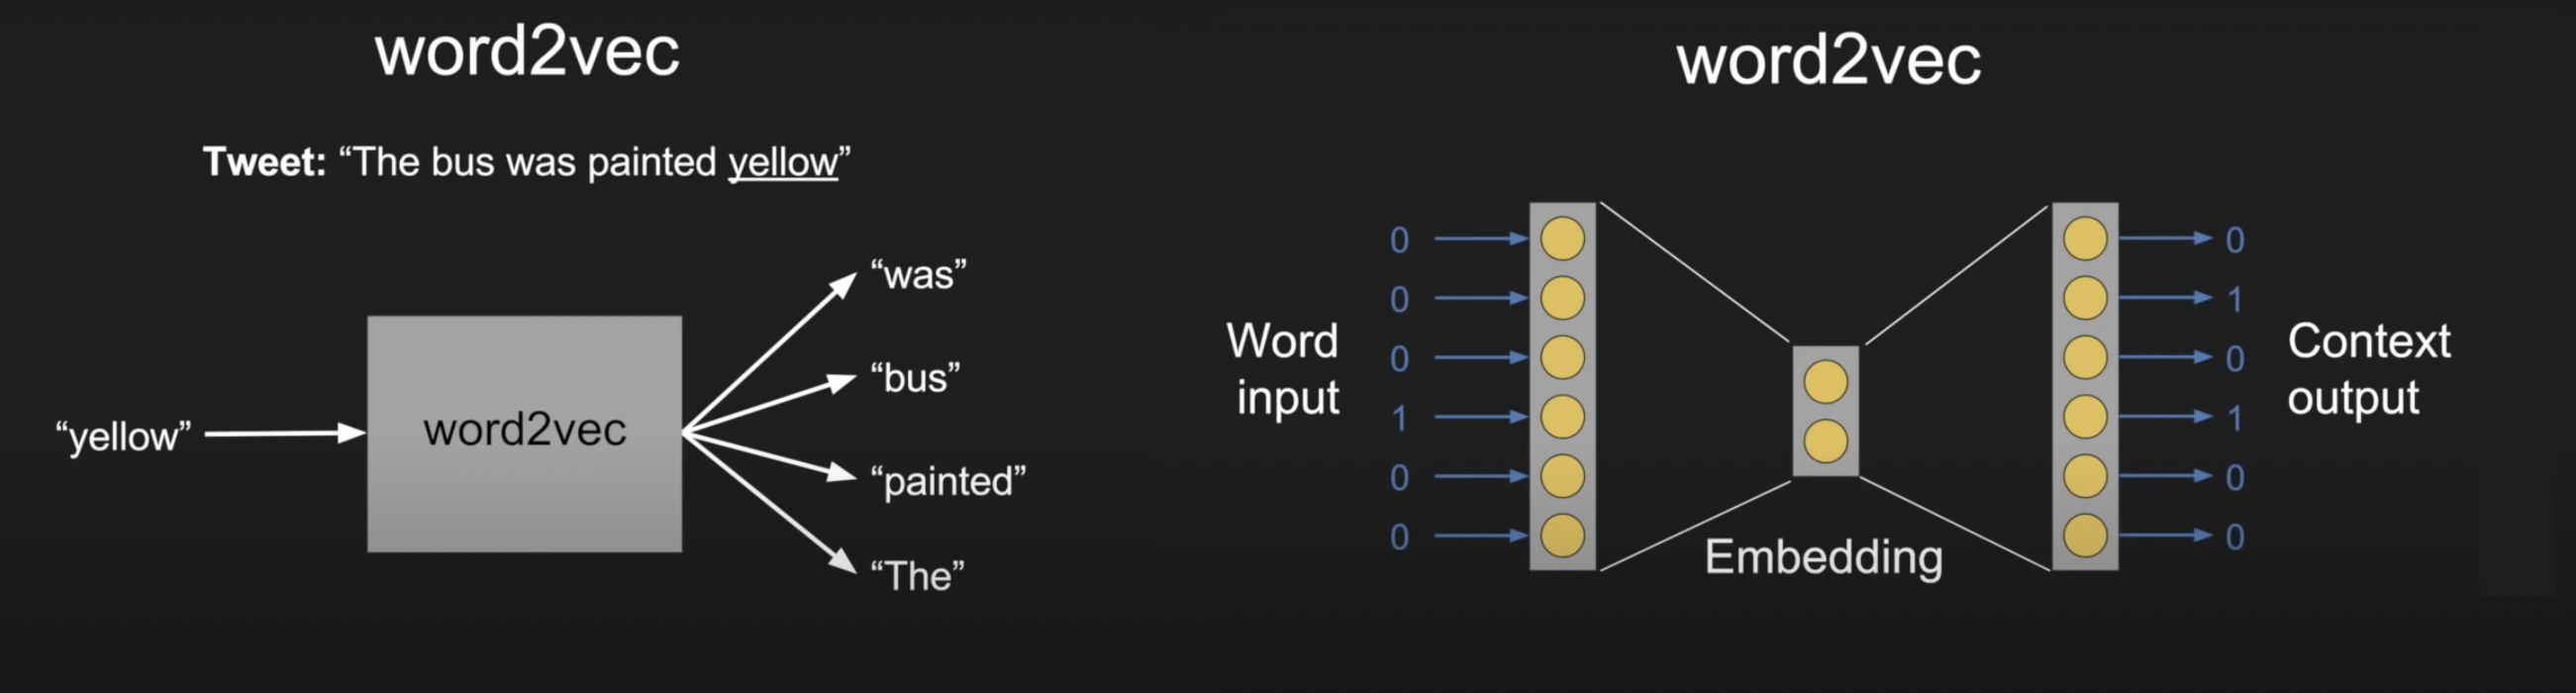
\includegraphics[width=0.8\columnwidth]{img/word2vec.png}
                \caption{Prediction-based word embeddings\footnotemark.}
                \label{fig:prediction-based-word-embeddings}
            \end{figure}
            \footnotetext{Source: \href{https://www.youtube.com/watch?v=5PL0TmQhItY&ab\_channel=macheads101}{https://www.youtube.com/watch?v=5PL0TmQhItY&ab\_channel=macheads101}}
        \end{answer}

        \item Most word embedding algorithms are based on the assumption that words that appear in similar contexts have similar meanings. What are some of the problems with context-based word embeddings?
        \begin{answer}
            \textit{Context size}. Using too small of a context window can result in inferring fewer relationships between the words, but using too large of a context window can result in every word being in the context of the other words. 

            \textit{Co-occurrence doesn't imply similarity}. Just because words occur together in a sentence often doesn't necessarily mean that the two words have the same meaning. For example, it might be the case that ``really'' and ``like'' occur frequently together, thereby being grouped closely in embedding space, but the meanings of the words are rather different. 

            \textit{Polysemy}. Traditionally, word embeddings don't account for polysemy -- words having multiple meanings based on the context. For example, in the sentence "The club I tried yesterday was great!", it is not clear if the term club is related to the word sense of a club sandwich, baseball club, clubhouse, golf club, or any other sense that club might have. 
        \end{answer}
    \end{InnerQandA}

    \item Given 5 documents:
    \begin{enumerate}[label=D\arabic*:]
        \item The duck loves to eat the worm
        \item The worm doesn’t like the early bird
        \item The bird loves to get up early to get the worm
        \item The bird gets the worm from the early duck
        \item The duck and the birds are so different from each other but one thing they have in common is that they both get the worm
    \end{enumerate}
    \begin{InnerQandA}
        \item Given a query Q: ``The early bird gets the worm'', find the two top-ranked documents according to the TF/IDF rank using the cosine similarity measure and the term set \{bird, duck, worm, early, get, love\}. Are the top-ranked documents relevant to the query?
        \begin{table}[h!]
            \centering
            \begin{tabular}{|c|cccccc|c|cccccc|}
            \hline
            \multirow{2}{*}{} & \multicolumn{6}{c|}{TF}                                                                                                                    & \multirow{2}{*}{IDF} & \multicolumn{6}{c|}{TF-IDF}                                                                                                                      \\ \cline{2-7} \cline{9-14} 
                              & \multicolumn{1}{c|}{D1}  & \multicolumn{1}{c|}{D2}  & \multicolumn{1}{c|}{D3}  & \multicolumn{1}{c|}{D4}  & \multicolumn{1}{c|}{D5}  & Q   &                      & \multicolumn{1}{c|}{D1}   & \multicolumn{1}{c|}{D2}   & \multicolumn{1}{c|}{D3}   & \multicolumn{1}{c|}{D4}   & \multicolumn{1}{c|}{D5}   & Q    \\ \hline
            bird              & \multicolumn{1}{c|}{0}   & \multicolumn{1}{c|}{1/3} & \multicolumn{1}{c|}{1/5} & \multicolumn{1}{c|}{1/5} & \multicolumn{1}{c|}{1/4} & 1/4 & log(5/4) = 0.22      & \multicolumn{1}{c|}{0}    & \multicolumn{1}{c|}{0.07} & \multicolumn{1}{c|}{0.04} & \multicolumn{1}{c|}{0.04} & \multicolumn{1}{c|}{0.05} & 0.05 \\ \hline
            duck              & \multicolumn{1}{c|}{1/3} & \multicolumn{1}{c|}{0}   & \multicolumn{1}{c|}{0}   & \multicolumn{1}{c|}{1/5} & \multicolumn{1}{c|}{1/4} & 0   & log(5/3) = 0.51      & \multicolumn{1}{c|}{0.17} & \multicolumn{1}{c|}{0}    & \multicolumn{1}{c|}{0}    & \multicolumn{1}{c|}{0.1}  & \multicolumn{1}{c|}{0.12} & 0    \\ \hline
            worm              & \multicolumn{1}{c|}{1/3} & \multicolumn{1}{c|}{1/3} & \multicolumn{1}{c|}{1/5} & \multicolumn{1}{c|}{1/5} & \multicolumn{1}{c|}{1/4} & 1/4 & log(5/5) = 0.00         & \multicolumn{1}{c|}{0}    & \multicolumn{1}{c|}{0}    & \multicolumn{1}{c|}{0}    & \multicolumn{1}{c|}{0}    & \multicolumn{1}{c|}{0}    & 0    \\ \hline
            early             & \multicolumn{1}{c|}{0}   & \multicolumn{1}{c|}{1/3} & \multicolumn{1}{c|}{1/5} & \multicolumn{1}{c|}{1/5} & \multicolumn{1}{c|}{0}   & 1/4 & log(5/3) = 0.51      & \multicolumn{1}{c|}{0}    & \multicolumn{1}{c|}{0.17} & \multicolumn{1}{c|}{0.1}  & \multicolumn{1}{c|}{0.1}  & \multicolumn{1}{c|}{0}    & 0.12 \\ \hline
            get               & \multicolumn{1}{c|}{0}   & \multicolumn{1}{c|}{0}   & \multicolumn{1}{c|}{1/5} & \multicolumn{1}{c|}{1/5} & \multicolumn{1}{c|}{1/4} & 1/4 & log(5/3) = 0.51      & \multicolumn{1}{c|}{0}    & \multicolumn{1}{c|}{0}    & \multicolumn{1}{c|}{0.1}  & \multicolumn{1}{c|}{0.1}  & \multicolumn{1}{c|}{0.12} & 0.12 \\ \hline
            love              & \multicolumn{1}{c|}{1/3} & \multicolumn{1}{c|}{0}   & \multicolumn{1}{c|}{1/5}  & \multicolumn{1}{c|}{0}   & \multicolumn{1}{c|}{0}   & 0   & log(5/2) = 0.91      & \multicolumn{1}{c|}{0.3}  & \multicolumn{1}{c|}{0}    & \multicolumn{1}{c|}{0.18} & \multicolumn{1}{c|}{0}    & \multicolumn{1}{c|}{0}    & 0    \\ \hline
            \end{tabular}
            \caption{TF-IDF scores for the 5 documents and the query}
            \label{tab:tf-idf-1}
            \end{table}
        \begin{answer}
            The calculations of the TF-IDF scores are given in Table \ref{tab:tf-idf-1}. Recall that:
            \begin{align*}
                \text{TF-IDF}(t, D) &= \text{TF}(t, D) \cdot \text{IDF}(t) \\
                \text{TF}(t, D) &= \text{freq}(t \in D) \\
                \text{IDF}(t) &= \log \left( \frac{\vert D \vert}{\vert \{ d \in D: t \in d \}\vert}\right)
            \end{align*}
            
            Now, we calculate the cosine similarities between the TF-IDF scores in order to obtain a ranking of the document similarity:
            \begin{align*}
                \cos \left( \text{Q}, \text{D1} \right) &= 0 \\
                \cos \left( \text{Q}, \text{D2} \right) &= 0.73 \\
                \cos \left( \text{Q}, \text{D3} \right) &= 0.63 \\
                \cos \left( \text{Q}, \text{D4} \right) &= 0.82 \\
                \cos \left( \text{Q}, \text{D5} \right) &= 0.54
            \end{align*}
            We obtain that the two most similar documents to Q are D4 and D2. However, one could argue that those two documents are not most relevant to the query Q, since D3 and D5 are semantically somewhat closer in meaning.
        \end{answer}

        \item Assume that document D5 goes on to tell more about the duck and the bird and mentions ``bird'' three times, instead of just once. What happens to the rank of D5? Is this change in the ranking of D5 a desirable property of TF/IDF? Why?
        \begin{answer}
            \notsure When one recalculates the TF-IDF scores for the modified document D5, it becomes apparent that the rankings do not change. 
        \end{answer}
    \end{InnerQandA}

    \item Your client wants you to train a language model on their dataset but their dataset is very small with only about 10,000 tokens. Would you use an n-gram or a neural language model?
    \begin{answer}
        Language models estimate the probability distribution over a sequence discrete tokens $x = (x_1, \ldots, x_T)$ as follows:
        \begin{align*}
            p(x) &= p(x_1, \ldots, x_T) \\
            &= p(x_1) p(x_2 \g x_1) \ldots p(x_T \g x_1, \ldots x_{T-1})
        \end{align*}
        where each token can take a value from a vocabulary $\mathcal{V}$.\\\\
        We can represent each conditional distribution with a probability table and learn the entries of these tables, but this becomes intractable as $T$ grows. For example, the probability table for $p(x_T \g x_1, \ldots x_{T-1})$ comprises of $\vert \mathcal{V}\vert^T$ entries. Therefore, huge memory and training sets are needed. \\\\
        Even if we use an n-gram, which is based on the Markov assumption -- thereby reducing $p(x_T \g x_1, \ldots x_{T-1})$ to $p(x_T \g x_{T-n+1}, \ldots x_{T-1})$, we still need tables as large as $\vert \mathcal{V} \vert^n$. \\\\
        Due to the exponential nature of the (non-parametric) n-gram model, we can easily suffer from the curse of dimensionality. Therefore, it might be a good idea to go with a neural language model, which operates in low-dimensional spaces and encodes smooth parametric functions for estimating the conditional distribution (instead of using large tables). The advantage is that these models typically scale linearly with $\vert V \vert$ and $n$. Moreover, since neural models also operate on word embeddings (instead of orthogonal one-hot encodings), modeling the relationships between the context and the target becomes an easier task. \\\\
        Of course, the small dataset of 10,000 tokens might not be large enough to train a sufficiently strong neural model, so it might be a good idea to try both approaches and see what works best.
    \end{answer}

    \item For n-gram language models, does increasing the context length (n) improve the model’s performance? Why or why not?
    \begin{answer}
        As we discussed above, by increasing n, the tables representing the conditional distributions $p(x_T \g x_{T-n+1}, \ldots x_{T-1})$ grow exponentially. In order to obtain meaningful representations, we'd need exponentially more datapoints, thereby falling into the trap of the curse of dimensionality.
    \end{answer}

    \item What problems might we encounter when using softmax as the last layer for word-level language models? How do we fix it?
    \begin{answer}
        This is already answered in Question 5, Section 7.2.
    \end{answer}

    \item What's the Levenshtein distance of the two words ``doctor'' and ``bottle''?
    \begin{answer}
         The Levenshtein distance between two words is the minimum number of single-character edits (i.e. insertions, deletions or substitutions) required to change one word into the other.\\\\
         In this case, the Levenshtein distance between ``doctor'' and ``bottle'' is 4:
         \begin{enumerate}[label=\arabic*.]
             \item Change d into b 
             \item Change c into t
             \item Change o into l
             \item Change r into e
         \end{enumerate}
    \end{answer}

    \item BLEU is a popular metric for machine translation. What are the pros and cons of BLEU?
    \begin{answer}
        BLEU (bilingual evaluation understudy) is an algorithm for evaluating the quality of text which has been machine-translated from one natural language to another. Quality is considered to be the correspondence between a machine's output and that of a human: "the closer a machine translation is to a professional human translation, the better it is" – this is the central idea behind BLEU. BLEU was one of the first metrics to claim a high correlation with human judgements of quality, and remains one of the most popular automated and inexpensive metrics.\\\\
        Scores are calculated for individual translated segments—generally sentences—by comparing them with a set of good quality reference translations. Those scores are then averaged over the whole corpus to reach an estimate of the translation's overall quality. Intelligibility or grammatical correctness are not taken into account.\\\\
        BLEU's output is always a number between 0 and 1. This value indicates how similar the candidate text is to the reference texts, with values closer to 1 representing more similar texts. Few human translations will attain a score of 1, since this would indicate that the candidate is identical to one of the reference translations. For this reason, it is not necessary to attain a score of 1. Because there are more opportunities to match, adding additional reference translations will increase the BLEU score.\\\\
        The advantages of BLEU are:
        \begin{itemize}
            \item Fast and simple to compute. 
            \item Widely used in both industry and academia.
        \end{itemize}
        In contrast, its disadvantages are:
        \begin{itemize}
            \item Doesn't consider meaning.
            \item Doesn't incorporate sentence structure.
            \item Struggles with non-English languages.
            \item Hard to compare scores with different tokenizers.
        \end{itemize}

        (Source: \href{https://en.wikipedia.org/wiki/BLEU}{Wikipedia}, \href{https://www.youtube.com/watch?v=M05L1DhFqcw}{HuggingFace})
    \end{answer}

    \item On the same test set, LM model A has a character-level entropy of 2 while LM model A has a word-level entropy of 6. Which model would you choose to deploy?
    \begin{answer}
        \todo 
        
        (Source: \href{https://thegradient.pub/understanding-evaluation-metrics-for-language-models/}{Chip Huyen's blog})
    \end{answer}

    \item Imagine you have to train a NER (Named Entity Recognition) model on the text corpus A. Would you make A case-sensitive or case-insensitive?
    \begin{answer}
        Unlike German, where all nouns are typically capitalised, in English capitalisation is a strong indicator for a named entity. Therefore, it might be a good idea to make the corpus case-sensitive. 

        (See more \href{https://stackoverflow.com/questions/56384231/case-sensitive-entity-recognition}{here})
    \end{answer}

    \item Why does removing stop words sometimes hurt a sentiment analysis model?
    \begin{answer}
        It is very likely that the corpus contains the stop word ``not'', which is a negation that can alter the valence of the passage. Therefore, removing this stop word will likely change/affect the context of the sentence, leading to ambiguity in the sentiment analysis.
    \end{answer}

    \item Many models use relative position embedding instead of absolute position embedding. Why is that?
    \begin{answer}
        Absolute position embedding impose a limit on the number of tokens a model can process. In contrast, relative position embedding is not dependent on the input size and can process sequences of variable length. 
    \end{answer}

    \item Some NLP models use the same weights for both the embedding layer and the layer just before softmax. What’s the purpose of this?
    \begin{answer}
        \textit{Weight Tying} improves the performance of language models by tying (sharing) the weights of the embedding and softmax layers. This method also massively reduces the total number of parameters in the language models that it is applied to.\\\\
        Language models are typically comprised of an embedding layer, followed by a number of Transformer or LSTM layers, which are finally followed by a softmax layer. Embedding layers learn word representations, such that similar words (in meaning) are represented by vectors that are near each other (in cosine distance). [Press \& Wolf, 2016] showed that the softmax matrix, in which every word also has a vector representation, also exhibits this property. This leads them to propose to share the softmax and embedding matrices, which is done today in nearly all language models.\\\\
        Additionally, [Press \& Wolf, 2016] propose Three-way Weight Tying, a method for NMT models in which the embedding matrix for the source language, the embedding matrix for the target language, and the softmax matrix for the target language are all tied. That method has been adopted by the Attention Is All You Need model and many other neural machine translation models.

        (Source: \href{https://paperswithcode.com/method/weight-tying}{PapersWithCode}; See more \href{https://tomroth.com.au/weight_tying/}{here})
    \end{answer}
\end{QandA}

\subsection{Computer vision}
\begin{QandA}
    \item For neural networks that work with images like VGG-19, InceptionNet, you often see a visualization of what type of features each filter captures. How are these visualizations created?
    \begin{answer}
        \textit{Feature visualization} answers questions about what a network (or parts of it) is looking for by generating examples. Neural networks are generally differentiable with respect to their inputs. Therefore, if we want to find out what kind of input would cause a certain behavior -- whether that's an internal neuron firing or the final output behavior -- we can use derivatives to iteratively tweak the input towards that goal. If we want to understand individual features, we can search for examples where they have high values -- either for a neuron at an individual position, a layer, or an entire channel (see Figure \ref{fig:feature-visualization})

        (Source: \href{https://distill.pub/2017/feature-visualization/}{DistillPub})
    \end{answer}
    \begin{figure}[h!]
        \centering
        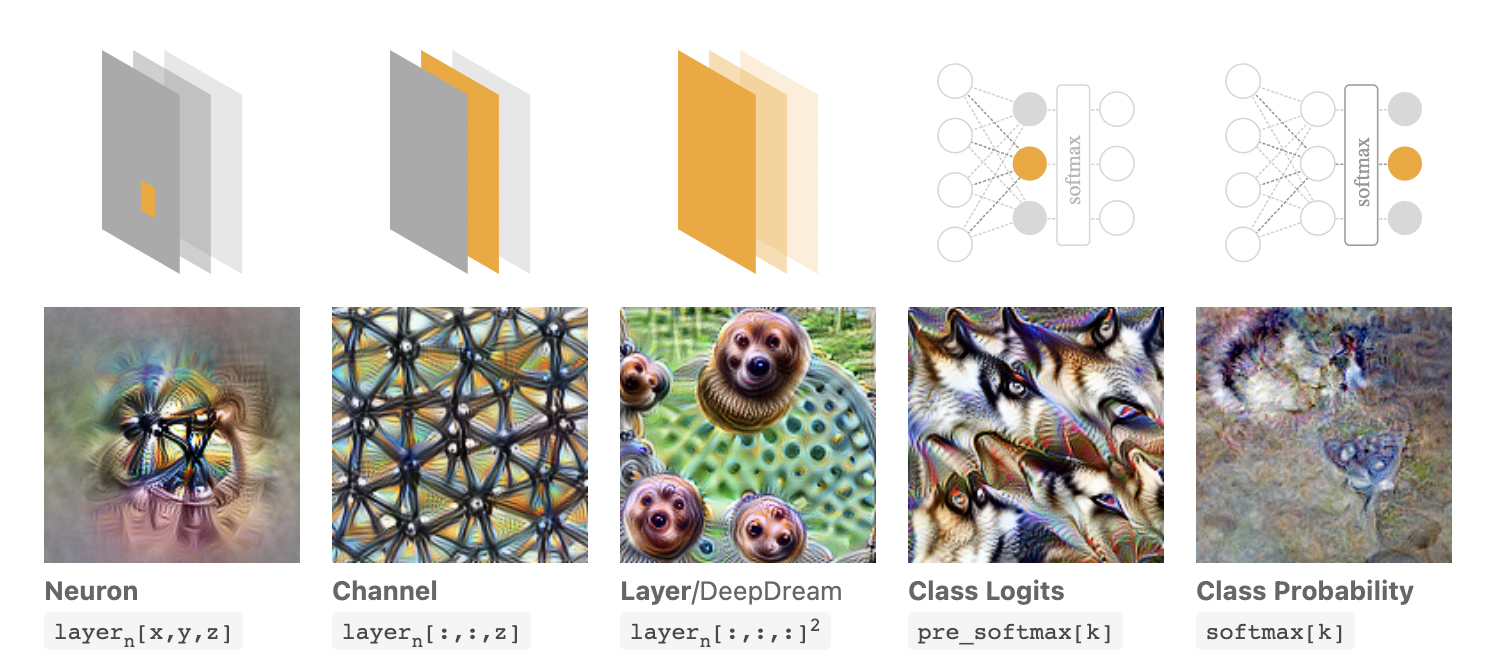
\includegraphics[width=0.7\columnwidth]{img/feature-visualization.png}
        \caption{Feature visualization}
        \label{fig:feature-visualization}
    \end{figure}

    \item Filter size
    \begin{InnerQandA}
        \item How are your model’s accuracy and computational efficiency affected when you decrease or increase its filter size?
        \begin{answer}
            Increasing the filter size results in decrease in computational efficiency (since the number of model parameters increases), and an increase in accuracy up to a certain point beyond which the network can overfit and imitate a fully-connected network. \\\\
            Alternatively, decreasing the filter size results in increase of computational efficiency, and a decrease in accuracy when tending towards using extremely small kernels (e.g. 1x1) which do not capture the local structure of the inputs properly.
        \end{answer}

        \item How do you choose the ideal filter size?
        \begin{answer}
            First of all, even-sized filters are not typical used because they break the symmetry around the neuron we are computing the local features for. Since 1x1 filters are too noisy and don't capture local dependencies, and 5x5 filters are rather computationally expensive, it has been empirically shown that 3x3 filters combine the best of both worlds: low computation cost and high accuracy.
        \end{answer}
    \end{InnerQandA}

    \item Convolutional layers are also known as ``locally connected''. Explain what it means.
    \begin{answer}
        Each filter operates only on a small neighborhood (e.g 3x3) around the ground pixel, and is applied across the entire spatial domain. This sort of weight sharing drastically reduces the number of the parameters, and injects the ``spatial equivariance'' bias.
    \end{answer}

    \item When we use CNNs for text data, what would the number of channels be for the first conv layer?
    \begin{answer}
        The number of input channels for the first conv layer will be the embedding dimensionality of the words.
    \end{answer}

    \item What is the role of zero padding?
    \begin{answer}
        By applying the convolution operation, we slightly reduce the size of the input image. In order to retain the same size, we append a border of zeros around the image.
    \end{answer}

    \item Why do we need upsampling? How to do it?
    \begin{answer}
        If pixel-level outputs are desired, we have to upsample the features again. Downsampling provides strong features with large receptive field; upsampling yields output at the same resolution as input. There are several strategies for upsampling:
        \begin{itemize}
            \item \textit{Nearest neighbor}: scale each neuron using nearest neighbor interpolation.
            \item \textit{Bilinear}:  scale each channel using bilinear neighbor interpolation.
            \item \textit{Bed of nails}: insert elements at sparse location (followed by convolution).
            \item \textit{Max unpooling}: remember which position was maximum during pooling, and insert the new element in the same location. Requires corresponding pairs of downsampling and upsampling layers.
        \end{itemize}
        Alternatively, instead of first downsampling and then upsampling, we can use \textit{dilated convolutions} in order to reach a large receptive field size quickly. Dilated convolutions increase the receptive field of standard convolutions without increasing the number of parameters.
    \end{answer}

    \item What does a 1x1 convolutional layer do?
    \begin{answer}
        The purpose of a 1x1 conv layer is to reduce the number of channels in the input activation volume. 
    \end{answer}

    \item Pooling.
    \begin{InnerQandA}
        \item What happens when you use max-pooling instead of average pooling?
        \begin{answer}
            Both techniques are non-parametric methods to reduce the spatial dimension (and in turn, increase the receptive field) of the input, with the difference being that max pooling outputs the maximum activation per patch, and average pooling outputs the average over all activations in the patch. 
        \end{answer}

        \item When should we use one instead of the other?
        \begin{answer}
            Given the above answer, we can postulate that max pooling extracts only the most salient features of the data, whereas average pooling smoothly extracts all features. Intuitively, average pooling encourages the network to identify the complete extent of the object, whereas max pooling restricts it to only the most important features, and ignores the noise/details. With that said, depending on how noisy or salient the inputs are, we might choose to go for the latter or the former pooling technique.
        \end{answer}

        \item What happens when pooling is removed completely?
        \begin{answer}
            The main purpose of the pooling operation is to increase the receptive field of the network by non-parametric techniques. If pooling is completely removed, then we'd need an increasingly large stack of convolutional layers to achieve large enough receptive fields for the neurons located in the deep layers. Of course, this comes at the cost of drastically increasing the number of parameters and computation requirements.
        \end{answer}

        \item What happens if we replace a 2x2 max pool layer with a conv layer of stride 2?
        \begin{answer}
            For this question, I will assume the max pool layer also has a stride of 2, and the conv layer has a single filter size of $2 \times 2$. \\\\
            The max pool layer merely operates on the spatial dimension, and works on each channel independently. Therefore, the output is of shape: $(W/2, H/2, C)$, and the number of parameters is $0$. \\\\
            In contrast, the conv layer will span over the entire channel dimension, resulting in the output: $(W/2, H/2, 1)$; however, the number of parameters is $1 \times 2 \times 2 \times C$. 
        \end{answer}
    \end{InnerQandA}

    \item When we replace a normal convolutional layer with a depthwise separable convolutional layer, the number of parameters can go down. How does this happen? Give an example to illustrate this.
    \begin{answer}
        Imagine we have an input image of shape $12 \times 12 \times 3$, and we want to apply $256$ filters of size $5 \times 5$, thereby obtaining an output volume of size $8 \times 8 \times 256$. \\\\
        In standard convolution, we  directly apply 256 filters of size $5 \times 5 \times 3$, where each filter spans the entire input channel dimension (which in this case is 3). \\\\
        In contrast, depthwise separable convolution splits this operation in two parts:
        \begin{itemize}
            \item First, we slide $3$ filters of size $5 \times 5 \times 1$ across the spatial domain of each of the $3$ input channels independently. The output of this operation is $8 \times 8 \times 3$. 
            \item Then, on the output of the previous operation, we apply $256$ filters of size $1 \times 1 \times 3$. The final output is therefore $8 \times 8 \times 256$, as desired.
        \end{itemize}
        Now, notice that in the standard convolution the number of parameters is $5 \times 5 \times 3 \times 256 = 19200$, whereas in the depthwise separable convolution the number of parameters is $5 \times 5 \times 3 + 3 \times 256 = 843$. The difference in the number of parameters is evident. \\\\
        Nevertheless, the reduction in model size comes at a cost of loss in expressivity. The intuition is as follows: in the standard convolution operation we transform the input volume $256$ times independently, whereas in the depthwise separable convolution we transform the input volume per-channel only once, and only then extend it to $256$ dimensions.

        (Source: \href{https://towardsdatascience.com/a-basic-introduction-to-separable-convolutions-b99ec3102728#:~:text=The%20depthwise%20separable%20convolution%20is,image%20may%20have%20multiple%20channels.}{TowardsDataScience})
    \end{answer}

    \item Can you use a base model trained on ImageNet (image size 256 x 256) for an object classification task on images of size 320 x 360? How?
    \begin{answer}
        Typically convnets have a global average pooling layer at the end of the stack of convolutional layers (and right before the stack of fully connected layers). The purpose of this layer is to reduce an activation volume of size $C \times W \times H$ down to $C \times 1 \times 1$ by computing the average of all values along the spatial dimension for each channel. Therefore, no matter the input image size, the spatial dimension at the end will be averaged out, and thus the fully connected layers will receive a fixed size input as expected.
    \end{answer}

    \item How can a fully-connected layer be converted to a convolutional layer?
    \begin{answer}
        Suppose the output volume of the stack of convolution layers has a shape of $W \times H \times C$.  Moreover, say we want to apply a fully-connected layer on this volume, and turn it into $T$ dimensional vector representation.\\\\
        Now, notice that instead of first flattening the input and then applying a linear transformation which consists of $(W \times H \times C) \times T$ parameters, we can directly apply a convolution operation with $T$ filters of size $W \times H$ (under the implicit assumption that the filter spans the entire channel dimension $C$). Again, the number of parameters is same: $T \times W \times H \times C$, with the only difference being the shape of the output: $1 \times 1 \times T$ (instead of simply $T$).

        (Source: \href{https://www.youtube.com/watch?v=XdsmlBGOK-k}{DeepLearningAI})
    \end{answer}

    \item Pros and cons of FFT-based convolution and Winograd-based convolution.
    \begin{answer}
        \todo
    \end{answer}
\end{QandA}

\subsection{Reinforcement Learning}
\begin{QandA}
    \item Explain the explore vs exploit tradeoff with examples.
    \begin{answer}
        In probability theory and machine learning, the \textit{multi-armed bandit problem} is a problem in which a fixed limited set of resources must be allocated between competing (alternative) choices in a way that maximizes their expected gain, when each choice's properties are only partially known at the time of allocation, and may become better understood as time passes or by allocating resources to the choice. This is a classic reinforcement learning problem that exemplifies the exploration–exploitation tradeoff dilemma. The name comes from imagining a gambler at a row of slot machines, who has to decide which machines to play, how many times to play each machine and in which order to play them, and whether to continue with the current machine or try a different machine.\\\\
        In the problem, each machine provides a random reward from a probability distribution specific to that machine, that is not known a-priori. The objective of the gambler is to maximize the sum of rewards earned through a sequence of lever pulls. The crucial tradeoff the gambler faces at each trial is between "exploitation" of the machine that has the highest expected payoff and "exploration" to get more information about the expected payoffs of the other machines. In practice, multi-armed bandits have been used to model problems such as managing research projects in a large organization, like a science foundation or a pharmaceutical company.
        
        (Source: \href{https://en.wikipedia.org/wiki/Multi-armed_bandit}{Wikipedia})
    \end{answer}

    \item How would a finite or infinite horizon affect our algorithms?
    \begin{answer}
        In reinforcement learning, an agent receives reward on each time step and the goal, loosely speaking, is to maximize the reward received. But that doesn’t actually fully define the goal, because each decision can affect what the agent can do in the future. Consequently, we’re left with the question “how does potential future reward affect our decision right now?”\\\\
        One answer is it doesn’t! We might say the objective is to only maximize the reward you’ll receive immediately for your next action, and ignore the consequences of how that affects your ability to receive reward after that. When your define the objective this way, you’ve defined the objective to be over a \textit{finite horizon}, where horizon refers to how many steps into the future the agent cares about the reward it can receive. Specifically, in this case, we’ve defined a 1 step horizon objective since we only care about the next reward received.\\\\
        But we could define any arbitrary horizon we want as the objective. We could define a 2 step horizon, in which the agent makes a decision that will enable it to maximize the reward it will receive in the next 2 time steps. Or we could choose a 3, or 4, or n step horizon!\\\\
        Or, we could go even further and define an \textit{infinite horizon} objective in which the agent tries to maximize the reward it will receive infinitely far into the future; that is, the agent cares about all possible future rewards and makes its decision accordingly. \\\\
        Although that might sound strange, infinite horizon objectives are the most common kind of objective in reinforcement learning work. Typically, in infinite horizon problems the objective is to maximize the discounted infinite horizon reward, which means the value of rewards further away in time successively matter less to the agent. Discounting has the important property that the best possible infinite horizon value is finite itself, allowing the agent to compare the relative value of different decisions.\\\\
        So when someone says “finite horizon” what they mean is describing the value the agent can achieve over only a finite number of steps into the future from its current state, rather than an infinite horizon, in which the agent cares about reward over all possible future steps.

        (Source: \href{https://www.quora.com/What-is-a-finite-horizon-in-the-context-of-reinforcement-learning}{Quora})
    \end{answer}

    \item Why do we need the discount term for objective functions?
    \begin{answer}
        From a theoretical perspective, using a discount rate (smaller than 1) is a mathematical trick to make an infinite sum finite. From a practical perspective, discount factors are associated with time horizons -- longer time horizons have have much more variance as they include more uncertainty about the future, while short time horizons are biased towards only short-term gains.

        (See more \href{https://stats.stackexchange.com/questions/221402/understanding-the-role-of-the-discount-factor-in-reinforcement-learning}{here})
    \end{answer}

    \item Fill in the empty circles using the minimax algorithm (see Figure \ref{fig:minimax}).
    
    \begin{figure}[h!]
        \centering
        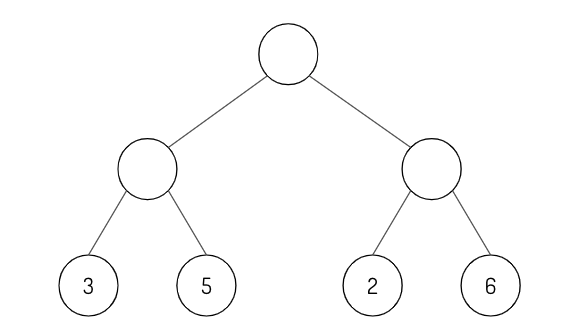
\includegraphics[width=0.5\columnwidth]{img/minimax.png}
        \caption{Minimax example}
        \label{fig:minimax}
    \end{figure}
    \begin{answer}
        The solution is provided in Figure \ref{fig:minimax-sol}.
    \end{answer}
    \begin{figure}[h!]
        \centering
        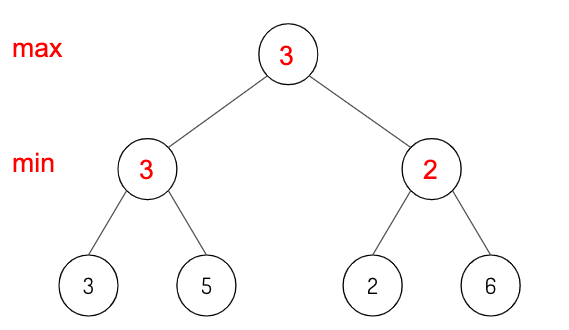
\includegraphics[width=0.5\columnwidth]{img/minimax-sol.png}
        \caption{Minimax solution}
        \label{fig:minimax-sol}
    \end{figure}

    \item Fill in the alpha and beta values as you traverse the minimax tree from left to right (see Figure \ref{fig:alpha-beta}).
    \begin{figure}[h!]
        \centering
        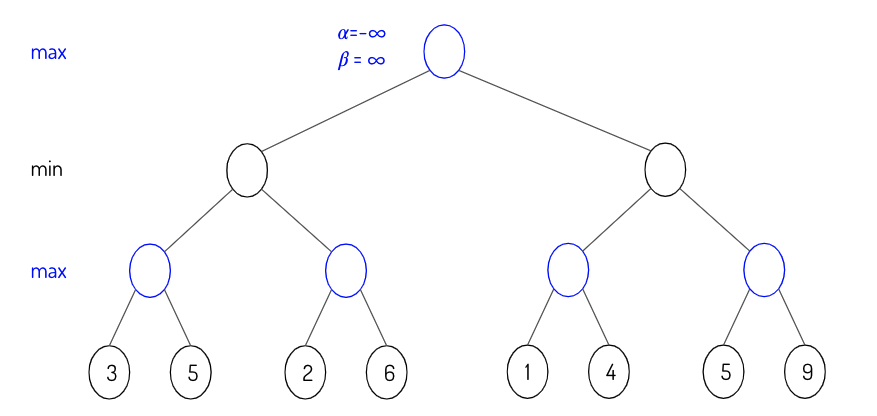
\includegraphics[width=0.7\columnwidth]{img/alpha-beta.png}
        \caption{Alpha-beta pruning example}
        \label{fig:alpha-beta}
    \end{figure}

    \begin{answer}
        The solution is provided in Figure \ref{fig:alpha-beta-sol}.
    \end{answer}

    \begin{figure}[h!]
        \centering
        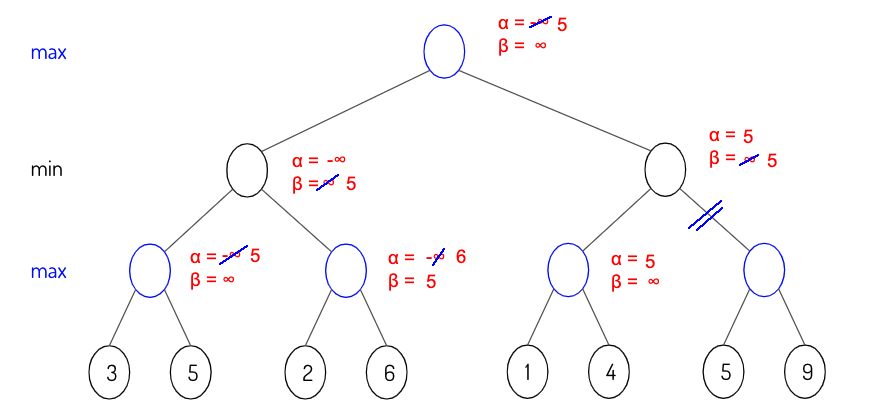
\includegraphics[width=0.7\columnwidth]{img/alpha-beta-sol.png}
        \caption{Alpha-beta pruning solution}
        \label{fig:alpha-beta-sol}
    \end{figure}

    \item Given a policy, derive the reward function.
    \begin{answer}
        \todo
    \end{answer}

    \item Pros and cons of on-policy vs. off-policy.
    \begin{answer}
        We consider an algorithm on-policy if it navigates the environment with the policy that is currently being learnt. In contrast, an off-policy algorithm uses a different policy for navigating the environment. \\\\
        Suppose we collect experience by executing a small number of policies $\pi_1, \ldots, \pi_N$ in a desired Markov environment. These could be existing policies that are known to be fairly good, or they could be exploration policies that seek to explore the state and action space well. In either case, we collect our experiences of the form of $(s_t, a_t, r_t, s_{t+1})$ tuples, where $s_t$ is the state of the environment at time $t$, $a_t$ is the action that was executed, $r_t$ is the reward that was received, and $s_{t+1}$ is the resulting state. Suppose we now want to evaluate a new policy $\tilde{\pi}$ to estimate its expected cumulative discounted reward. We could do this by executing $\tilde{\pi}$ in the real environment, but usually that is expensive and could lead to large losses in the real world (such as a robot car striking a pedestrian or crashing into a wall). Instead we would like to evaluate $\tilde{\pi}$ using the collected experience. This is off-policy policy evaluation.\\\\
        Off-policy learning seeks to find a good (or even optimal) policy by doing a series of off-policy policy evaluations. Suppose $\pi_\theta$ is a policy that is defined by a set of weights, $\theta$. For example, $\pi_\theta$ could be a neural network for choosing actions. Using off-policy policy evaluation, we can estimate both the expected value (cumulative discounted reward) of $\pi_\theta$ and also its gradient with respect to $\theta$. Then we can update $\theta$ by taking a step in the direction of the gradient and repeat. \\\\
        Off-policy evaluation is not as accurate as on-policy evaluation. If the policy $\tilde{\pi}$ that we are evaluating is very different from the initial policies $\pi_1, \ldots, \pi_N$ that were used to collect experience, then we cannot obtain a very accurate estimate of its value. In such cases, we need to collect more “on policy” experience by executing $\tilde{\pi}$ in the real Markov environment.\\\\
        In summary, off-policy evaluation is faster since it only involves computation, and is safer since it doesn't require acting in the real world. However, it is less accurate than on-policy evaluation.

        (Source: \href{https://www.quora.com/What-are-the-benefits-of-using-off-policy-learning-over-on-policy-learning-in-reinforcement-learning}{Quora})
    \end{answer}

    \item What’s the difference between model-based and model-free? Which one is more data-efficient?
    \begin{answer}
        The main difference between model-based and model-free agents is whether during learning or acting, the agent uses predictions of the environment response. \\\\
        Model-based agents can ask ask the model for a single prediction about the next state and reward, or the full distribution of next states and rewards. These predictions can be provided entirely outside of the learning agent (e.g. by computer code that understands the rules of a dice or board game), or they can be learned by the agent (in which case they will be approximate).\\\\
        Algorithms that purely sample from experience such as Monte Carlo Control, SARSA, Q-learning, Actor-Critic are "model free" RL algorithms. They rely on real samples from the environment and never use generated predictions of next state and next reward to alter behaviour (although they might sample from experience memory, which is close to being a model).\\\\
        The archetypical model-based algorithms are Dynamic Programming (Policy Iteration and Value Iteration) -- these all use the model's predictions or distributions of next state and reward in order to calculate optimal actions. Specifically in Dynamic Programming, the model must provide state transition probabilities, and expected reward from any (state, action) pair. Note this is rarely a learned model. \\\\
        Basic TD learning is also model-based -- in order to pick the best action, it needs to query a model that predicts what will happen on each action, and implement a policy as follows:
        \begin{align*}
            \pi(s) = \argmax_{a} \sum_{s', r} p(s', r \g s, a) (r + V(s'))
        \end{align*}
        where $p(s', r \g s, a)$ serves as the model.\\\\
        In general, model-based agents are more data-efficient since you can relate the sparsely available samples to the inner built model. 
        
        (Source: \href{https://ai.stackexchange.com/questions/4456/whats-the-difference-between-model-free-and-model-based-reinforcement-learning}{StackExchange})
    \end{answer}
\end{QandA}

\subsection{Other (from deep learning architectures and applications)}
\begin{QandA}
    \item An autoencoder is a neural network that learns to copy its input to its output. When would this be useful?
    \begin{answer}
        There are several applications of autoencoders:
        \begin{itemize}
            \item \textit{Dimensionality reduction}. By creating a bottleneck in the network predicting its input, we are effectively learning a compressed/low-dimensional representation of our data, which we might go on to use in other applications, such as classification, anomaly detection, deep metric learning, etc.
            \item \textit{Image denoising}. The idea is to first corrupt the input image with noise (e.g. Gaussian), and then predict the non-corrupted image as the ground truth. That way, we can learn representations that are more robust to noise. 
            \item \textit{Generative modeling}. Variational Autoencoders (VAEs) introduce a sampling mechanism at the bottleneck of the model which allows for a more structured representation of the latent space, and generating high-fidelity samples. 
        \end{itemize}
    \end{answer}

    \item Self-attention.
    \begin{InnerQandA}
        \item What’s the motivation for self-attention?
        \begin{answer}
            Say the following sentence is an input sentence we want to translate: ``The animal didn't cross the street because it was too tired''. \\\\
            What does “it” in this sentence refer to? Is it referring to the street or to the animal? It’s a simple question to a human, but not as simple to an algorithm. When the model is processing the word “it”, self-attention allows it to associate “it” with “animal”. \\\\
            As the model processes each word (each position in the input sequence), self attention allows it to look at other positions in the input sequence for clues that can help lead to a better encoding for this word.\\\\
            If you’re familiar with RNNs, think of how maintaining a hidden state allows an RNN to incorporate its representation of previous words/vectors it has processed with the current one it’s processing. Self-attention is the method the Transformer uses to bake the “understanding” of other relevant words into the one we’re currently processing.

            (Source: \href{https://jalammar.github.io/illustrated-transformer/}{Jay Alammar's blog})
        \end{answer}

        \item Why would you choose a self-attention architecture over RNNs or CNNs?
        \begin{answer}
            Like recurrent neural networks (RNNs), transformers are designed to process sequential input data, such as natural language, with applications towards tasks such as translation and text summarization. However, unlike RNNs, transformers process the entire input all at once. The attention mechanism provides context for any position in the input sequence. For example, if the input data is a natural language sentence, the transformer does not have to process one word at a time. This allows for more parallelization than RNNs and therefore reduces training times.

            (Source: \href{https://en.wikipedia.org/wiki/Transformer\_(machine\_learning\_model)}{Wikipedia})
        \end{answer}

        \item Why would you need multi-headed attention instead of just one head for attention?
        \begin{answer}
            Consider the sentence: ``I kicked the ball''. Notice that the sentence has a causal structure: ``I (who?) kicked (did what?) the ball (to whom?)''. \\\\
            Using a single attention head wouldn't be able to disambiguate the three pieces of information since it is a convex combination of the vector representations. \\\\
            Therefore, instead of using a single overparametrized attention head, the authors suggest to use multiple smaller heads which would be able to learn the different concepts without entanglement. 

            (See more \href{https://www.youtube.com/watch?v=5vcj8kSwBCY}{here})
        \end{answer}

        \item How would changing the number of heads in multi-headed attention affect the model’s performance?
        \begin{answer}
            As we discussed in the previous question, it is of crucial importance to use more than one head, as it increases the expressivity of the Transformer. \\\\
            However, setting too many heads might cause duplication of information, overfitting, and entanglement of sentence structures.  \\\\
            Nevertheless, this is a hyperparameter that can be searched over -- the authors of the paper ``Attention is All You Need'' found that using 8 heads was optimal for the problem of machine translation. 
        \end{answer}
    \end{InnerQandA}

    \item Transfer learning
    \begin{InnerQandA}
        \item You want to build a classifier to predict sentiment in tweets but you have very little labeled data (say 1000). What do you do?
        \begin{answer}
            It would be a good idea to take a pre-trained model (e.g. BERT), and fine tune it on our limited dataset.
        \end{answer}

        \item What’s gradual unfreezing? How might it help with transfer learning?
        \begin{answer}
            A common practice in DL is to take large pretrained models achieving state-of-the-art results on many benchmarks, and fine tune them to some other downstream application. Nevertheless, naive fine-tuning can result in catastrophic forgetting, and overfitting to the new dataset. Gradual unfreezing tackles this problem by gradually unfreezing the layers (usually starting from the deeper layers) in order to prevent catastrophic forgetting of the knowledge learned during the source task.
        \end{answer}
    \end{InnerQandA}

    \item Bayesian methods.
    \begin{InnerQandA}
        \item How do Bayesian methods differ from the mainstream deep learning approach?
        \begin{answer}
            In deep learning, we mostly aim to optimize the weights $W$ by maximizing the likelihood of the data $p(Y \g X, W)$. In contrast, Bayesian methods assume posterior distribution on the weights $p(W \g X, Y)$ which is often learnt through an approximate parametric formulation $q(W \g X, Y)$ due to intractability -- a process known as Variational Inference. Another approach of estimating the posterior is through sampling, which is arguably a  much more expensive technique.
        \end{answer}

        \item How are the pros and cons of Bayesian neural networks compared to the mainstream neural networks?
        \begin{answer}
            The advantage of Bayesian Neural Nets is that they provide a natural notion of uncertainty for the prediction, which is quite useful in fields like medicine, biology, aerospace, etc.\\\\
            Nevertheless, at this time, this comes at the cost of decrease in accuracy compared to standard neural nets, difficulty to scale to large problems, the ambiguity of choosing a proper prior, etc.
        \end{answer}

        \item Why do we say that Bayesian neural networks are natural ensembles?
        \begin{answer}
            The reason why they are natural ensembles is because we can average the predictions from all possible weight configurations, scaled by the probability of each configuration occurring:
            \begin{align*}
                p(Y \g X) &= \int_w p(Y, W \g X) dw \\
                &= \int_w p(Y \g X, W) p(W) dw
            \end{align*}
        \end{answer}
    \end{InnerQandA}

    \item GANs.
    \begin{InnerQandA}
        \item What do GANs converge to?
        \begin{answer}
            Let $x \in \R^D$ denote an observation and $p(z)$ a prior over latent variables $z \in \R^Q$. Moreover, let $G_{w_G}: \R^Q \rightarrow \R^D$ denote the generator network with induced distribution $p_{model}$, and $D_{w_D}: \R^D \rightarrow \left[ 0, 1\right]$ denote the discriminator network which outputs a probability of a sample being real or not. \\\\
            $D$ and $G$ play the following  two-player minimax game with value function $V(G, D)$:
            \begin{align*}
                G^*, D^* &= \argmin_{G} \argmax_{D} V(D, G) \\
                V(D, G) &= \mathbb{E}_{x \sim p_{data}(x)}\left[ \log D(x) \right] + \mathbb{E}_{z \sim p(z)} \left[\log \left( 1 - D(G(z)) \right) \right]
            \end{align*}
            We train $D$ to assign probability 1 to samples from $p_{data}$ and 0 to samples from $p_{model}$; whereas we train $G$ to fool $D$ such that it assigns probability 1 to samples from $p_{model}$.\\\\
            It can be shown that for any generator $G$, the optimal discriminator $D^*$ is:
            \begin{align*}
                D^*_{G}(x) = \frac{p_{data}(x)}{p_{data}(x) + p_{model}(x)}
            \end{align*}
            Now, let's explore what happens to the value function $V$ when we are at $D^*$:
            \begin{align*}
                V(G, D^*_G) &= \mathbb{E}_{x \sim p_{data}} \left[ \log D^*_G(x) \right] + \mathbb{E}_{x \sim p_{model}} \left[\log(1 - \left( D^*_G (x) \right)) \right] \\
                &= \mathbb{E}_{x \sim p_{data}} \left[ \log \frac{p_{data}(x)}{p_{data}(x) + p_{model}(x)}\right] + \mathbb{E}_{x \sim p_{model}} \left[ \log \frac{p_{model}(x)}{p_{data}(x) + p_{model}(x)}\right] \\
                &= \KL{p_{data}}{p_{data} + p_{model}} + \KL{p_{model}}{p_{data} + p_{model}}  \\
                &= -\log4 + \log4 + \KL{p_{data}}{p_{data} + p_{model}} + \KL{p_{model}}{p_{data} + p_{model}} \\
                &= -\log 4 + \KL{p_{data}}{\frac{p_{data} + p_{model}}{2}} + \KL{p_{model}}{\frac{p_{data} + p_{model}}{2}} \\
                &= -\log 4 + \text{JSD}\left[  p_{data}, p_{model} \right]
            \end{align*}
            where JSD is the Jenson Shannon Divergence. Since this is a non-negative quantity, when $G$ tries to minimize $V(G, D^*_G)$ it will push $\text{JSD}\left[  p_{data}, p_{model}\right]$ down to 0, which is achieved for $p_{model} = p_{data}$. In turn, this implies:
            \begin{align*}
                D^*_{G}(x) &= \frac{p_{data}(x)}{p_{data}(x) + p_{model}(x)} \underbrace{=}_{p_{model} = p_{data}} = \frac{1}{2} \\
                V(G*, D^*_G) &= -\log 4 + \text{JSD}\left[  p_{data}, p_{model} \right] \underbrace{=}_{p_{model} = p_{data}} -\log4
            \end{align*}
        \end{answer}

        \item Why are GANs so hard to train?
        \begin{answer}
            One major failure mode of GANs is mode collapse, where the generator learns to produce high-quality sample with very low variability, covering only a fraction of $p_{data}$. Consider the example in Figure \ref{fig:mode-collapse}:
            \begin{enumerate}[label=\arabic*.]
                \item The generator learns to fool the discriminator by producing values close to Antarctic temperatures. 
                \item The discriminator can't distinguish Antarctic temperatures, but learns that all Australian temperatures are real.
                \item The generator learns that it should produce Australian temperatures and abandons the Antarctic mode. 
                \item The discriminator can't distinguish Australian temperatures, but learns that all Antarctic temperatures are real. 
                \item Repeat.
            \end{enumerate}
            \begin{figure}[h!]
                \centering
                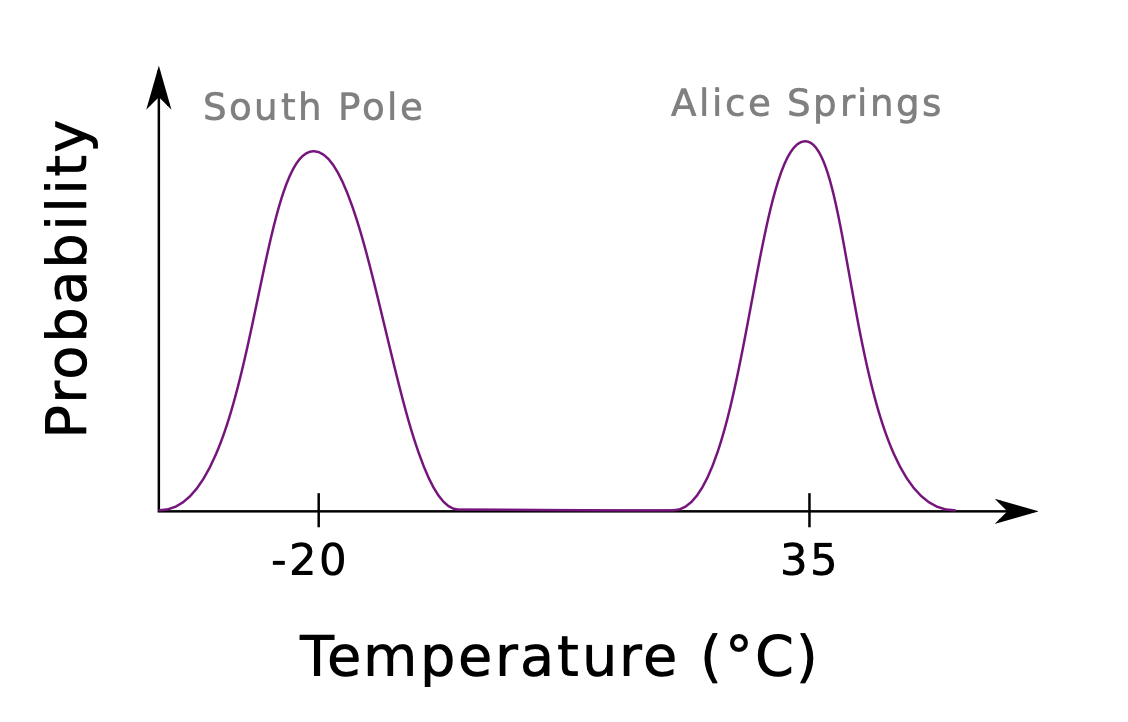
\includegraphics[width=0.5\linewidth]{img/mode-collapse.png}
                \caption{Mode collapse example}
                \label{fig:mode-collapse}
            \end{figure}

            There are several strategies for avoiding mode collapse:
            \begin{itemize}
                \item \textit{Encourage diversity}: Minibatch discrimination allows the discriminator to compare samples across a batch to determine whether the entire batch is real or fake (as opposed to single samples).
                \item \textit{Anticipate counterplay}: Look into the future (e.g. via unrolling the discriminator), and anticipate counterplay when updating generator parameters.
                \item \textit{Experience replay}: Hopping back and forth between modes can be minimised by showing old fake samples to the discriminator once in a while.
                \item \textit{Multiple GANs}: Train multiple GANs and hope they cover all modes.
                \item \textit{Different optimization objective}: Wasserstein GANs, Gradient penalties
            \end{itemize}
        \end{answer}
    \end{InnerQandA}
\end{QandA}

\subsection{Training neural networks}
\begin{QandA}
    \item When building a neural network, should you overfit or underfit it first?
    \begin{answer}
        When building a neural network, it is almost always a good idea to overfit to the data, in order to make sure that the model is actually capable of learning. If the model cannot overfit even on few (e.g. 5) samples, then it is very likely we have a bug in the implementation. Once we make sure that we can overfit to the data, we can gradually increase the dataset and employ regularization techniques. 
    \end{answer}

    \item Write the vanilla gradient update.
    \begin{answer}
        \begin{enumerate}[label=\arabic*.]
            \item Initialize weights $w^0$ and pick learning rate $\alpha$
            \item For all data points $i \in \{1, \ldots, N\}$ do:
            \begin{enumerate}[label=2.\arabic*.]
                \item Forward propagate $x_i$ through the network to calculate predictions $\hat{y}_i$
                \item Backpropagate to obtain gradient $\nabla_w \mathcal{L}_i (w^t, y_i, \hat{y}_i)$
            \end{enumerate}
            \item Update weights: $w^{t+1} = w^t - \alpha \frac{1}{N}\sum_{i=1}^N \nabla_w \mathcal{L}_i(w^t, y_i, \hat{y}_i)$
            \item If validation error decreases go to step 2, otherwise stop.
        \end{enumerate}
    \end{answer}

    \item Neural network in simple NumPy.
    \begin{InnerQandA}
        \item Write in plain NumPy the forward and backward pass for a two-layer feed-forward neural network with a ReLU layer in between.
        \begin{answer}
            A typical neural network will have the following computation graph:
            \begin{align*}
                Z^{[l]} &= W^{[l]} A^{[l-1]} \\
                A^{[l]} &= g(Z^{[l]}) \\
                \mathcal{L} &= \left( A^{[L]} - Y \right)^2
            \end{align*}
            where $A^{[0]} = X$ is the input to the net, $A^{[L]}$ is the output of the net, and $g$ is an activation function. Accordingly, the gradients can be derived as follows (see more \href{https://edwardshu.com/posts/matrix-matrix-gradient}{here} and \href{https://towardsdatascience.com/lets-code-a-neural-network-in-plain-numpy-ae7e74410795}{here}):
            \begin{align*}
                dZ^{[l]} &= dA^{[l]} \odot g'(Z^{[l]}) \\
                dW^{[l]} &= dZ^{[l]} A^{[l-1]t} \\
                dA^{[l-1]} &= W^{[l]t} dZ^{[l]}
            \end{align*}
            The computation graph for our task will look as follows:
            \begin{align*}
                Z^{[1]} &= W^{[1]}X \\
                A^{[1]} &= \text{ReLU}(Z^{[1]}) \\
                Z^{[2]} &= W^{[2]} A^{[1]} \\
                \mathcal{L} &= \left( Z^{[2]} - Y \right)^2
            \end{align*}
            Accordingly, the gradients can be computed as follows:
            \begin{align*}
                dZ^{[2]} &= 2(Z^{[2]} - Y)\\
                dW^{[2]} &= dZ^{[2]} A^{[1]t} \\
                dA^{[1]} &= W^{[2]t} dZ^{[2]} \\ 
                dZ^{[1]} &= dA^{1} \odot \text{ReLU}' (Z^{[1]}) \\
                dW^{[1]} &= dZ^{[1]} X^t
            \end{align*}
            where $\text{ReLU}'(Z) = Z \odot \mathbbm{1}_{Z \ge 0}$. The code implementation in NumPy is available \href{https://gist.github.com/zaf-stojano/136b6cc1675bb0e14972d937c390b7a6}{here}, \textit{completely} generated by yours truly -- Github CoPilot.
        \end{answer}

        \item Implement vanilla dropout for the forward and backward pass in NumPy.
        \begin{answer}
            The updated version of the gist with dropout can be found \href{https://gist.github.com/zaf-stojano/0cda51a7a1068d2936de3f1df2a47332}{here}. This time CoPilot needed a bit hand-holding, but is still very impressive.
        \end{answer}
    \end{InnerQandA}

    \item Activation functions.
    \begin{InnerQandA}
        \item Draw the graphs for sigmoid, tanh, ReLU, and leaky ReLU.
        \begin{answer}
            The activation functions are drawn in Figure \ref{fig:activation-functions}.
        \end{answer}
        \begin{figure}[h!]
                \centering
                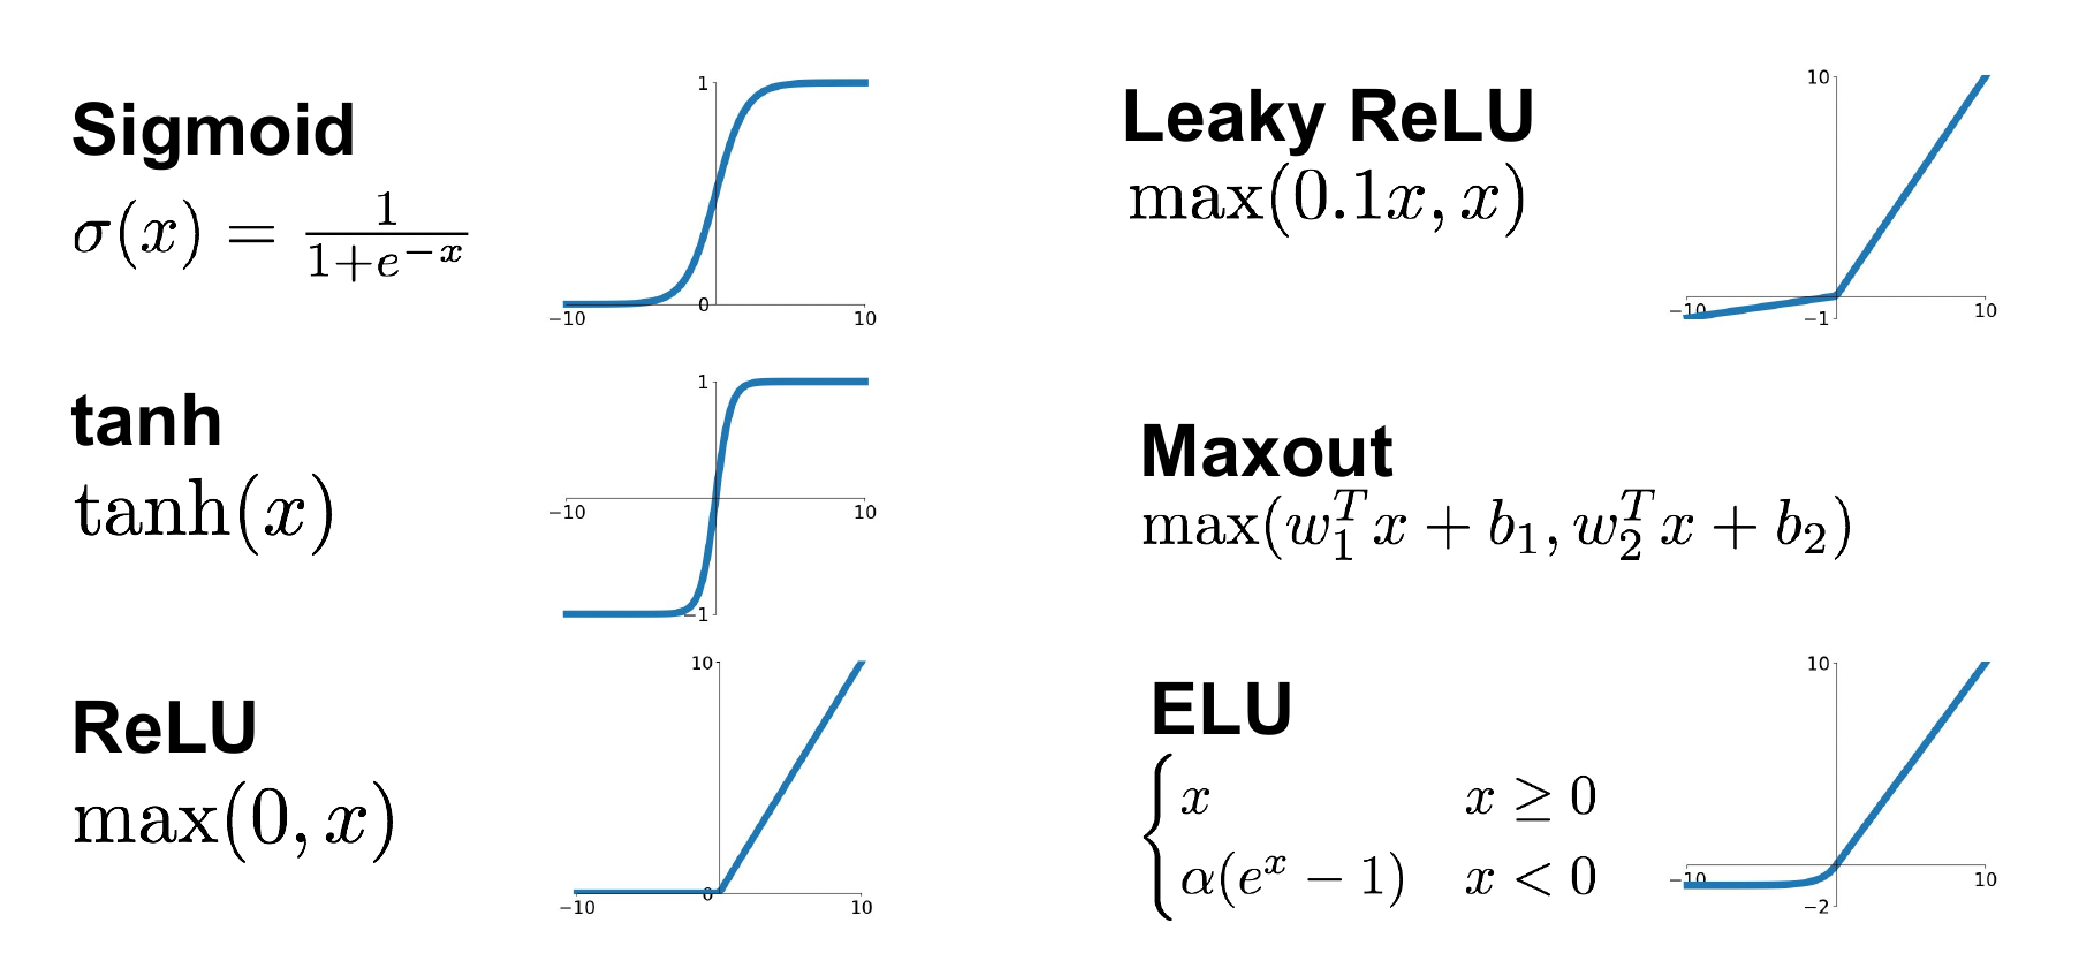
\includegraphics[width=0.7\linewidth]{img/activation-functions.png}
                \caption{Activation functions}
                \label{fig:activation-functions}
            \end{figure}

        \item Pros and cons of each activation function.
        \begin{answer}
            \begin{itemize}
                \item sigmoid. Pros: bounded output, natural notion of producing probabilities as range is between 0 and 1. Cons: saturation for very large/small inputs, introduces bias as outputs are not zero-centered.
                \item tanh. Pros: bounded, zero-centered. Cons: saturation for very large/small inputs.
                \item ReLU. Pros: does not saturate for $x > 0$, leads to faster convergence, computationally efficient. Cons: Not zero-centered, no learning for $x < 0$ (dead ReLU's).
                \item Leaky ReLU. Pros: Doesn't saturate, outputs closer to zero-centered, fast convergence, computationally efficient. Cons: not perfectly zero-centered, gradients still very small for negative inputs close to zero (see how GeLU solves this problem for inputs around 0). 
            \end{itemize}
        \end{answer}

        \item Is ReLU differentiable? What to do when it’s not differentiable?
        \begin{answer}
            While ReLU is not differentiable at 0, we can use a faux gradient as follows:
            \begin{align*}
                \frac{\partial}{\partial x} \text{ReLU}(x) = \begin{cases}
                    x &\text{if } x \ge 0 \\
                    0 &\text{otherwise}
                \end{cases}
            \end{align*}
        \end{answer}

        \item Derive derivatives for sigmoid function $\sigma(x)$  when $x$ is a vector.
        \begin{answer}
            Previously, for $x \in \R$ we proved that:
            \begin{align*}
                \frac{\partial }{\partial x} \sigma(x) = \sigma(x)(1-\sigma(x))
            \end{align*}
            Since the activation function is applied element-wise, then the derivative when $x$ is a vector generalizes to a Hadamard product:
            \begin{align*}
                \frac{\partial }{\partial x} \sigma(x) = \sigma(x) \otimes (1-\sigma(x))
            \end{align*}
        \end{answer}
    \end{InnerQandA}

    \item What’s the motivation for skip connection in neural works?
    \begin{answer}
        During the forward pass, through the skip connections we manage to inject knowledge from the earlier layers towards the latter layers (e.g. positional encodings in Transformers, which are only injected at the embeddings). Moreover, during the backward pass, the earlier layers do not learn a lot due to the vanishing gradient problem; therefore, by using the skip connections we can propagate gradients further back to the earlier layers.
    \end{answer}

    \item Vanishing and exploding gradients.
    \begin{InnerQandA}
        \item How do we know that gradients are exploding? How do we prevent it?
        \begin{answer}
            We might be suffering from exploding gradients if:
            \begin{itemize}
                \item The model is unable to get traction on your training data (e.g. poor loss).
                \item The model is unstable, resulting in large changes in loss from update to update.
                \item The model loss goes to NaN during training.
                \item The model weights go to NaN values during training.
            \end{itemize}
            In order to prevent exploding gradients, we can perform clipping:
            \begin{align*}
                \text{W.grad} = \begin{cases}
                  \text{W.grad} & \text{if } \Vert \text{W.grad} \Vert_2 \le \tau \\
                  \tau \frac{\text{W.grad}}{\Vert \text{W.grad} \Vert_2} & \text{otherwise}
                \end{cases}
            \end{align*}
            where $\tau$ is a hyper-parameter s.t $\tau \in \left[1, 10\right]$.

            (Source: \href{https://machinelearningmastery.com/exploding-gradients-in-neural-networks/}{MachineLearningMastery})
        \end{answer}

        \item Why are RNNs especially susceptible to vanishing and exploding gradients?
        \begin{answer}
            Consider an RNN cell with one-dimensional hidden state $h \in \R$ and a one-dimensional input $x \in \R$. Then:
            \begin{align*}
                h_t = \text{tanh} \left(w_h h_{t-1} + w_x x_t + b \right)
            \end{align*}
            When performing backpropagation through time, we need to compute the quantity:
            \begin{align*}
                \frac{\partial h_t}{\partial h_{t-k}} &= \frac{\partial h_t}{\partial h_{t-1}} \frac{\partial h_{t-1}}{\partial h_{t-2}} \cdots \frac{\partial h_{t-k+1}}{\partial h_{t-k}} \\
                &= \left( (\text{tanh}_t)' \cdot w_h \right) \left( (\text{tanh}_{t-1})' \cdot w_h \right) \ldots \left( (\text{tanh}_{t-k+1})' \cdot w_h \right) \\
                &= \left(\prod_{i=t-k+1}^t (\text{tanh}_{i})' \right) (w_h)^k  
            \end{align*}
            First, if we don't carefully initialize the weights, we might end up with saturating activation functions, that is $(\text{tanh}_i)' \approx 0$, implying that $\frac{\partial h_t}{\partial h_{t-k}} \approx 0 $. \\\\
            Given that we carefully initialize the weights we have $\text{tanh}(x) \approx x$ (no saturation), or more precisely:
            \begin{align*}
                h_t &= \text{tanh} \left(w_h h_{t-1} + w_x x_t + b \right) \\
                &\approx w_h h_{t-1} + w_x x_t + b
            \end{align*}
            Now, let us again observe the gradient:
            \begin{align*}
                \frac{\partial h_t}{\partial h_{t-k}} &= \frac{\partial h_t}{\partial h_{t-1}} \frac{\partial h_{t-1}}{\partial h_{t-2}} \cdots \frac{\partial h_{t-k+1}}{\partial h_{t-k}} \\
                &= w_h \cdot w_h \ldots  w_h \\
                &= (w_h)^k  
            \end{align*}
            For $w_h > 1$ the gradients will explode -- for example, if $w_h = 1.1$ and $k = 100$ we have $\frac{\partial h_t}{\partial h_{t-k}} = (w_h)^k = 13781$. \\\\
            On the other hand, for $w_h < 1$ the gradients will vanish -- for example, if $w_h = 0.9$ and $k = 100$ we have $\frac{\partial h_t}{\partial h_{t-k}} = (w_h)^k = 0.0000266$.
        \end{answer}
    \end{InnerQandA}

    \item Weight normalization separates a weight vector’s norm from its gradient. How would it help with training?
    \begin{answer}
        % First of all, I believe there might be an error in the question: weight normalization separates a weight vector's norm from its \textbf{direction}. With that said, let's dive in the answer.\\\\
        \todo
    \end{answer}

    \item When training a large neural network, say a language model with a billion parameters, you evaluate your model on a validation set at the end of every epoch. You realize that your validation loss is often lower than your train loss. What might be happening?
    \begin{answer}
        There are several possible reasons as to why the validation loss is lower than the training loss:
        \begin{itemize}
            \item It might be that the training loss uses regularizers (e.g. L2 norm on the weights). Since at validation time we only evaluate the main loss function, it might happen that the validation loss is lower than the (composite) train loss. 
            \item The model might have dropout layers, which impose heavy regularization during training. These are layers that behave differently during training (dropping out neurons) and inference time (no dropping out neurons, but multiplying weights by dropout probability to imitate ensembling). 
            \item The validation set might simply be easier compared to the train set.
        \end{itemize}
    \end{answer}

    \item What criteria would you use for early stopping?
    \begin{answer}
        We can perform early stopping if there is no change or a decrease in a metric of interest (validation loss, accuracy, etc.). It is a good idea to use a patience parameter in order to avoid noisy estimates. 
    \end{answer}

    \item Gradient descent vs SGD vs mini-batch SGD.
    \begin{answer}
        \begin{itemize}
            \item In gradient descent we first perform a forward pass and a backward pass for each sample in the dataset, before we take a step in the direction of the cumulative gradient. This is extremely slow to converge, as today's datasets are extremely large in size, which implies that we perform gradient updates too rarely. 
            \item In SGD, after performing a forward and a backward pass for a single sample, we take a step in the direction of the single gradient. Even though we perform gradient updates much more often, the entire process is extremely noisy as we are optimizing with respect to a single sample at a time. 
            \item Mini-batch SGD combines the best of both worlds: perform a forward/backward pass for a batch (e.g. 32) of samples, and take a step in the direction of the gradient for the current mini-batch. On one hand, we perform updates more often than pure gradient descent; on the other hand, we optimize over an entire mini-batch, minimizing the noise in the estimated gradient. 
        \end{itemize}   
    \end{answer}

    \item It’s a common practice to train deep learning models using epochs: we sample batches from data without replacement. Why would we use epochs instead of just sampling data with replacement?
    \begin{answer}
        First of all, \href{https://leon.bottou.org/publications/pdf/slds-2009.pdf}{(Bottou et al, 2009)} empirically show that random shuffling before each epoch leads to faster convergence. On top of it, there are some practical reasons as to why one would not perform random draws with replacement:
        \begin{itemize}
            \item It's a well defined metric: "the neural network was trained for 10 epochs" is a clearer statement than "the neural network was trained for 18942 iterations" or "the neural network was trained over 303072 samples".
            \item There's enough randomness going on during the training phase: random weight initialization, mini-batch shuffling, dropout, etc.
            \item It is easy to implement.
            \item It avoids wondering whether the training set is large enough not to have epochs.
        \end{itemize}
        
        (Source: \href{https://stats.stackexchange.com/questions/242004/why-do-neural-network-researchers-care-about-epochs}{StackExchange})
    \end{answer}

    \item Your model’s weights fluctuate a lot during training. How does that affect your model’s performance? What to do about it?
    \begin{answer}
        Let us look at the gradient update of the weights:
        \begin{align*}
            w^{t+1} = w^t - \alpha \nabla_w \mathcal{L}(w^t)
        \end{align*}
        The fluctuation can be attributed to two primary factors: large learning rate or exploding gradients. In either case, this can seriously destabilize the training process. In order to resolve this issue, we could: 1) lower the learning rate; 2) perform gradient clipping. 
    \end{answer}

    \item Learning rate.
    \begin{InnerQandA}
        \item Draw a graph number of training epochs vs training error for when the learning rate is: i) too high; ii) too low; iii) acceptable.
        \begin{answer}
            The graph is depicted in Figure \ref{learning-rate-epochs}
        \end{answer}
        \begin{figure}[h!]
            \centering
            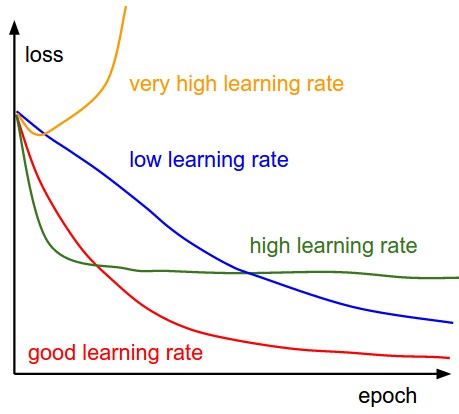
\includegraphics[width=0.5\linewidth]{img/learning-rate-epochs.jpeg}
            \caption{Epochs vs loss for various learning rates\footnotemark }
            \label{learning-rate-epochs}
        \end{figure}
        \footnotetext{Source \href{https://towardsdatascience.com/useful-plots-to-diagnose-your-neural-network-521907fa2f45}{https://towardsdatascience.com/useful-plots-to-diagnose-your-neural-network-521907fa2f45}}

        \item What’s learning rate warmup? Why do we need it?
        \begin{answer}
            Warmup steps are just a few updates with low learning rate at the beginning of training. After this warmup, you use the regular learning rate (schedule) to train your model to convergence.\\\\
            Intuitively, the idea that this helps your network to slowly adapt to the data. However, in practice the main reason for warmup steps is to allow adaptive optimizers (e.g. Adam, RMSProp, etc) to compute correct statistics of the gradients. Therefore, a warmup period makes little sense when training with plain SGD. \\\\
            For example, RMSProp computes a moving average of the squared gradients to get an estimate of the variance in the gradients for each parameter. For the first update, the estimated variance is just the square root of the sum of the squared gradients for the first batch. Since, in general, this will not be a good estimate, your first update could push your network in a wrong direction. To avoid this problem, you give the optimiser a few steps to estimate the variance while making as little changes as possible (low learning rate) and only when the estimate is reasonable, you use the actual (high) learning rate.

            (Source: \href{https://datascience.stackexchange.com/questions/55991/in-the-context-of-deep-learning-what-is-training-warmup-steps}{StackExchange})
        \end{answer}
    \end{InnerQandA}

    \item Compare batch norm and layer norm.
    \begin{answer}
        As an example we will use a fully-connected network, although the same reasoning can be applied to CNNs, Transformers, etc. \\\\
        Suppose the output of the previous layer is $X \in \R^{B \times D}$ where $B$ is the batch size and $D$ is the dimensionality of the embedding. Both techniques normalize the input as follows:
        \begin{align*}
            Y = \frac{X - \Exp{X}}{\sqrt{\Vari{X}} + \epsilon} * \gamma + \beta
        \end{align*}
        where $\gamma$ and $\beta$ are learnt affine parameters, and all operations are treated as broadcasts. The main difference stems from how the two techniques compute the statistics:
        \begin{itemize}
            \item \textit{Batch norm} computes the mean and standard deviation over the batch, meaning that $\Exp{X} \in \R^{1 \times D}$ and $\Vari{X} \in \R^{1 \times D}$.
            \item Layer norm computes the mean and standard deviation over the features, meaning that $\Exp{X} \in \R^{B \times 1}$ and $\Vari{X} \in \R^{B \times 1}$.
        \end{itemize}
    \end{answer}

    \item Why is squared L2 norm sometimes preferred to L2 norm for regularizing neural networks?
    \begin{answer}
        Both the L2 norm and the squared L2 norm provide the same optimization goal. However, the squared L2 norm is computationally more simple, as you don't have to calculate the square root. Moreover, when deriving the gradients by hand, the derivatives have a more easier form to work with. 
    \end{answer}

    \item Some models use weight decay: after each gradient update, the weights are multiplied by a factor slightly less than 1. What is this useful for?
    \begin{answer}
        Weight Decay, or $L_2$ Regularization, is a regularization technique applied to the weights of a neural network. We minimize a loss function compromising both the primary loss function and a penalty on the $L_2$ Norm of the weights:
        \begin{align*}
            \tilde{\mathcal{L}}(w) = \mathcal{L}(W) + \frac{\lambda}{2} w^t w
        \end{align*}
        where $\lambda$ is a hyperparameter determining the strength of the penalty. This encourages smaller weights, which prevents potential overfitting by allowing the network to arbitrarily closely fit the data. \\\\
        Let us now observe the implicit effect of weight decay when performing the update rule in the optimization procedure:
        \begin{align*}
            w^{t+1} &= w^t - \alpha \nabla_w \tilde{\mathcal{L}}(w^t) \\
            &= w^t - \alpha(\nabla_w \mathcal{L}(w^t) + \lambda w^t) \\
            &= (1 - \alpha \lambda)w^t - \alpha \nabla_w \mathcal{L}(w^t)
        \end{align*}
        In other words, since $\alpha > 0, \lambda > 0$, what we essentially do is we first slightly decay the weights, and then take a small step in the opposite direction of the gradient. \\\\
        Weight decay can be incorporated directly into the weight update rule, rather than just implicitly by defining it through to objective function. Often weight decay refers to the implementation where we specify it directly in the weight update rule (whereas L2 regularization is usually the implementation which is specified in the objective function). For example, see the PyTorch documentation on how the \href{https://pytorch.org/docs/stable/\lagenerated/torch.optim.SGD.html}{SGD} optimizer incorporates weight decay explicitly. 

        (Source: \href{https://paperswithcode.com/method/weight-decay}{PapersWithCode})
    \end{answer}    

    \item It’s a common practice for the learning rate to be reduced throughout the training
    \begin{InnerQandA}
        \item What’s the motivation?
        \begin{answer}
            The learning rate is controlling the size of the update steps along the gradient. This parameter sets how much of the gradient you update, with:
            \begin{itemize}
                \item Larger learning rate allowing the model converge faster, but may overstep the optimal point.
                \item Smaller learning rate being more receptive to the loss function, but may require more epochs to converge and may get stuck in local minima.
            \end{itemize}
            The learning rate schedule allows you to start training with larger steps and reduce the learning rate, in an effort to combine the best of both worlds.

            (Source: \href{https://peltarion.com/knowledge-center/modeling-view/run-a-model/optimization-principles-(in-deep-learning)/learning-rate-schedule}{Peltarion})
        \end{answer}

        \item What might be the exceptions?
        \begin{answer}
            An exception might be a continual learning scenario, where we continuously update the model with new data. In this case, if we constantly decrease the learning rate, the model will not learn from data further down the stream. On the other hand, if we use a scheduler with (warm) restarts, the alternation between small and large learning rates can further exacerbate the effects of catastrophic forgetting. Therefore, it might be the most optimal case to use a constant learning rate.
        \end{answer}
    \end{InnerQandA}

    \item Batch size.
    \begin{InnerQandA}
        \item What happens to your model training when you decrease the batch size to 1?
        \begin{answer}
            After performing a forward and a backward pass for a single sample, we take a step in the direction of the single gradient. Even though we perform gradient updates much more often, the entire process is extremely noisy as we are optimizing with respect to a single sample at a time.
        \end{answer}

        \item What happens when you use the entire training data in a batch?
        \begin{answer}
            After performing a forward pass and a backward pass for each sample in the dataset, we take a step in the direction of the cumulative gradient. This is extremely slow to converge, as today's datasets are extremely large in size, which implies that we perform gradient updates too rarely. 
        \end{answer}

        \item How should we adjust the learning rate as we increase or decrease the batch size?
        \begin{answer}
            When utilizing larger batches, we can afford to have large learning rates, as the approximated gradient of the batch is closer to the true gradient. On the other hand, using very small batches yields noisy estimates of the gradient, and is therefore advisable to also use small learning rates so that we don't diverge in our optimization procedure. 
        \end{answer}
    \end{InnerQandA}

    \item Why is Adagrad sometimes favored in problems with sparse gradients?
    \begin{answer}
        First, let us note that feature sparsity will induce gradient sparsity, simply due to the chain rule (the derivative of the weight is dependent on the value of the feature/activation). In turn, this can result in a lot of oscillation when performing the gradient update, since the direction will be dominated by the non-sparse gradients. \\\\
        In order to alleviate this problem, Adagrad proposes to use a scaled learning rate per weight, such that we move slower in the direction of a lot of oscillation (variance), and give more importance in the direction of sparsity. More precisely, the update rule is as follows:
        \begin{align*}
            G^t &= \sum_{i=1}^t \left(\nabla_w{\mathcal{L}(w^t)}\right) \left(\nabla_w{\mathcal{L}}(w^t)\right)^t \\
            w^{t+1} &= w^t - \frac{\alpha}{\sqrt{\text{diag}(G^t) + \epsilon I}} * \nabla_w \mathcal{L}(w^t)
        \end{align*}
        This way, we dampen gradients that have high variance; and give more weight to gradients with low variance (induced by the sparsity).

        (See more \href{https://towardsdatascience.com/learning-parameters-part-5-65a2f3583f7d}{here})
    \end{answer}

    \item Adam vs. SGD.
    \begin{InnerQandA}
        \item What can you say about the ability to converge and generalize of Adam vs. SGD?
        \begin{answer}
            \href{https://arxiv.org/abs/1705.08292}{(Wilson et al., 2017)} show that solutions found by adaptive methods (e.g. Adam) generalize worse than SGD, even when these solutions have better training performance. In other words, adaptive methods converge faster, but have worse generalization performance than pure SGD. 

            (See more \href{https://shaoanlu.wordpress.com/2017/05/29/sgd-all-which-one-is-the-best-optimizer-dogs-vs-cats-toy-experiment/}{here})
        \end{answer}

        \item What else can you say about the difference between these two optimizers?
        \begin{answer}
            Pure SGD performs gradient updates based on mini-batches instead of the entire dataset:
            \begin{align*}
                w^{t+1} = w^t - \alpha \nabla_w \mathcal{L}(w^t)
            \end{align*}
            One issue with it is that the learning rate scales the gradients equally in every direction. Therefore, if one direction dominates the gradient, the optimization procedure might oscillate a lot and take a lot longer to converge to the minimum. \\\\
            With this in mind, Adam aims to improve the convergence performance by: 1) operating on a momentum-updated version of the gradients; 2) dividing the momentum by the gradient variance; The goal of both terms is dampen the variance of the gradient. More precisely, the update step looks as follows:
            \begin{align*}
                m^{t+1} &= \beta_1 m^t + (1-\beta_1)\nabla_w \mathcal{L}(w^t) &\text{(momentum gradient)} \\
                v^{t+1} &= \beta_2 v^{t} + (1-\beta_2)(\nabla_w \mathcal{L}(w^t) \odot \nabla_w \mathcal{L}(w^t)) &\text{(uncentered variance)}  \\
                \hat{m}^{t+1} &= \frac{m^{t+1}}{1 - \beta_1^{t+1}} \quad\quad \hat{v}^{t+1} = \frac{v^{t+1}}{1 - \beta_2^{t+1}} &\text{(bias correction)} \\
                w^{t+1} &= w^t - \alpha \frac{\hat{m}^{t+1}}{\sqrt{\hat{v}^{t+1}} + \epsilon} & \text{(gradient step)}
            \end{align*}
        \end{answer}
    \end{InnerQandA}

    \item With model parallelism, you might update your model weights using the gradients from each machine asynchronously or synchronously. What are the pros and cons of asynchronous SGD vs. synchronous SGD?
    \begin{answer}
        \todo 
    \end{answer}

    \item Why shouldn’t we have two consecutive linear layers in a neural network?
    \begin{answer}
        Consider the following two-layer MLP:
        \begin{align*}
            h &= g(W_1 x + b_1) \\
            y &= g(W_2 h + b_2)
        \end{align*}
        which can be written as:
        \begin{align*}
            y = g(W_2 g(W_1 x + b_1) + b_2)
        \end{align*}
        Now, if we use linear activation function $g(x) = x$, observe that:
        \begin{align*}
            y = W_2 (W_1 x + b_1) + b_2 = W_2 W_1 x + W_2 b_1 + b_2 = W x + b
        \end{align*}
        In other words, the MLP can only express linear functions. 
    \end{answer}

    \item Can a neural network with only ReLU (non-linearity) act as a linear classifier?
    \begin{answer}
        I guess no, since I don't see how the network can produce valid probabilities with the ReLU activation function (unbounded from above). 
    \end{answer}

    \item Design the smallest neural network that can function as an XOR gate.
    \begin{answer}
        \begin{align*}
            \text{XOR}(x_1, x_2) = \text{AND} \left( \text{OR}(x_1, x_2), \text{NAND}(x_1, x_2) \right)
        \end{align*}
    \end{answer}

    \item Why don’t we just initialize all weights in a neural network to zero?
    \begin{answer}
        The problem of symmetry is not only present when we initialize the weights with zero, but also when we (in decreasing order of restrictiveness):
        \begin{itemize}
            \item Initialize all weight matrices with a constant.
            \item Initialize each weight matrix with a different constant
            \item Initialize each weight matrix such that all rows for a given matrix are the same. 
        \end{itemize}
        The issue with this sort of initialization is that all units in each layer will produce the same outputs. Therefore, during backpropagation, we will have the same local derivatives $\frac{\partial \mathcal{L}}{\partial z^{l}_i}$, which in turn will cause the weights for all neurons in a given layer to perform the same update. By induction, one can show that even after $n$ iterations of gradient descent we will preserve the symmetry, thus seriously straining the capacity of the network. 

        (See more \href{https://www.coursera.org/lecture/neural-networks-deep-learning/www.deeplearning.ai-XtFPI}{here})
    \end{answer}

    \item Stochasticity.
    \begin{InnerQandA}
        \item What are some sources of randomness in a neural network?
        \begin{answer}
            Random weight initialization, mini-batch shuffling, dropout, etc.
        \end{answer}

        \item Sometimes stochasticity is desirable when training neural networks. Why is that?
        \begin{answer}
            \begin{itemize}
                \item Random noise allows neural nets to produce multiple outputs given the same instance of input. For example, AlphaGo outputs probability of winning the game for every possible move, and chooses the next step by sampling with respect to these probabilities -- otherwise, the behavior of the agent is going to be highly deterministic.
                \item Random noise limits the amount of information flowing through the network, forcing the network to learn meaningful representations of data. For example, vanilla Autoencoders can easily overfit to the train data, thus not being able to generate samples with high fidelity. In contrast, Variational Autoencoders (VAEs) inject Gaussian noise in the bottleneck, thereby forcing the network to learn meaningful representations of the data. 
                \item Random noise provides "exploration energy" for finding better optimization solutions during gradient descent. For example, in Stochastic Gradient Descent (SGD) instead of navigating the loss landscape by computing the gradients over the entire dataset, we estimate the gradient by evaluating the network on a mini-batch of samples. This way, even if we get stuck in a local optima in one iteration, in the next it is very likely we escape it as we are always optimizing with respect to a ``proxy'' to the original loss.
            \end{itemize}

            (Source: \href{https://blog.evjang.com/2016/07/randomness-deep-learning.html}{Eric Jang's blog})
        \end{answer}
    \end{InnerQandA}

    \item Dead neuron.
    \begin{InnerQandA}
        \item What’s a dead neuron?
        \begin{answer}
            Suppose a neuron uses ReLU activation function. If the input to the activation function $z^l = w^t a^{l-1}$ is highly negative (perhaps due to weight initialization), then the output of the neuron is $0$. Since the gradient in this region is $0$, and due to the mechanics of the chain rule, the gradient backpropagated through this neuron will also be zero. As a result, the weights going into the neuron will not get updated, and the same behavior can persist over time, thereby deeming the neuron as ``dead''.

            (See more \href{https://datascience.stackexchange.com/questions/5706/what-is-the-dying-relu-problem-in-neural-networks}{here})
        \end{answer}

        \item How do we detect them in our neural network?
        \begin{answer}
            By observing the distribution of outputted values over time, we can detect neurons that have peak highly at certain values (e.g. 0).
        \end{answer}

        \item How to prevent them?
        \begin{answer}
            One way to tackle dead ReLU's is to instead use Leaky ReLU's, as they have small, but constant gradient for large negative inputs. 
        \end{answer}
    \end{InnerQandA}

    \item Pruning.
    \begin{InnerQandA}
        \item Pruning is a popular technique where certain weights of a neural network are set to 0. Why is it desirable?
        \begin{answer}
            In the context of artificial neural networks, pruning is the practice of removing parameters (which may entail removing individual parameters, or parameters in groups such as by neurons) from an existing network. The goal of this process is to maintain accuracy of the network while increasing its efficiency. This can be done to reduce the computational resources required to run the neural network.

            (Source: \href{https://en.wikipedia.org/wiki/Pruning\_(artificial\_neural\_network)}{Wikipedia})
        \end{answer}

        \item How do you choose what to prune from a neural network?
        \begin{answer}
            Typically, there are 2 techniques: 1) pruning weights; 2) pruning neurons. \\\\
            Weight-based pruning doesn't cause a large dip in performance, but might require special hardware to allow for efficient sparse computations.  On the other hand, neuron-based pruning allows the network to be run normally without sparse computation / special hardware, but might seriously strain the performance capabilities of the model. \\\\
            Nevertheless, in both cases the goal is to remove more of the less important parameters. Typical pruning criteria used in practice are:
            \begin{itemize}
                \item \textit{Magnitude}. Remove weights that have magnitude close to 0; remove neurons whose L2 norm of the weight is also close to 0.
                \item \textit{Activations}. We could also use the training data to observe the activations of the neurons. We can remove neurons whose distribution of  activations extremely peaked (invariant to the input); Moreover, we can also remove a neuron if its activation pattern is highly correlated to another neuron in the same layer. 
            \end{itemize}

            We repeat the pruning process until certain conditions are met -- dipping below a threshold accuracy, achieving certain memory size / computation time for the model, etc. Nonetheless, depending on the problem at hand, we might have to fine-tune the pruned model for a couple of iterations in order to improve the performance. 
            
            (Source: \href{https://towardsdatascience.com/pruning-neural-networks-1bb3ab5791f9}{TowardsDataScience})
        \end{answer}
    \end{InnerQandA}

    \item Under what conditions would it be possible to recover training data from the weight checkpoints?
    \begin{answer}
        In general, there are 2 main types of model inversion attacks:
        \begin{itemize}
            \item White-box, where we have access to the model checkpoints. In fact, today it is very common to open-source the model weights, on platforms such as PyTorch Hub, Hugging Face, etc. The main idea of white-box model inversion part is to fix the pre-trained network, and optimize the input (through back-propagation) with respect to a given confidence score.
            \item Black-box, where we can only query the model. This is the most typical scenario, as many services offer access to their model through an API. The main idea of black-box model inversion is to train a decoder network to recreate the input with which we query the online model, based on its outputted confidence scores / latent representation. 
        \end{itemize}
        
        (See more \href{https://blog.openmined.org/extracting-private-data-from-a-neural-network/}{here})
    \end{answer}

    \item Why do we try to reduce the size of a big trained model through techniques such as knowledge distillation instead of just training a small model from the beginning?
    \begin{answer}
        Empirically, given enough data larger models often outperform their smaller counterparts. Since the process of model distillation is related to compressing large models while still keeping nearly the same performance, there might be indication that the compressed model might also outperform the purely trained variant. \\\\
        One might even relate the idea to \href{https://twitter.com/AnthropicAI/status/1570087876053942272}{polysemanticity} -- the ability of neurons to pack many concepts in a single neuron. Since larger models are more expressive, distillation might provide a way of packing the knowledge of the larger models into a smaller one. In turn, this might lead to outperforming a purely trained small variant, simply due to the lack of expressivity of the small model. 
    \end{answer}
    
\end{QandA}

\end{document}
